\documentclass[a4paper, 11pt, twoside]{book}  % Use the "Thesis" style, based on the ECS Thesis style by Steve Gunn

\usepackage{amsfonts}
\usepackage{amsmath}
\usepackage{amssymb}
\usepackage{amstext}
\usepackage[utf8]{inputenc} %pdfLatex input french letter
\usepackage[T1]{fontenc}  %xelatex input french letter
\usepackage[french,american]{babel}
\usepackage{bm}
\usepackage{booktabs}
\usepackage{calc}
\usepackage{caption}
\usepackage{cases}
\usepackage{color}
\usepackage[colorlinks,linkcolor=blue,citecolor=blue,urlcolor=blue]{hyperref}
\usepackage{comment}
\usepackage{emptypage}

%\usepackage{enumitem}
\usepackage{enumerate}
%\usepackage{fontspec}
\usepackage{fancyhdr}
\usepackage{float}
\usepackage[top=2.5cm,bottom=2cm,left=3cm,right=2.5cm,headheight=15pt]{geometry}
\usepackage{graphicx}
\usepackage{grffile}  % better image filename handling
\usepackage{xspace}
\usepackage{newtxtext}
\usepackage{indentfirst}
\usepackage{lineno}  % cross-referencing related
\usepackage{mathtools}  % \coloneqq
\usepackage[framemethod=tikz]{mdframed}
\usepackage{amsthm}
\usepackage{minitoc}
\setcounter{minitocdepth}{2}
\usepackage{multirow,tabularx}
\usepackage[sort&compress]{natbib}  % Use the "Natbib" style for the references in the Bibliography
\usepackage{pdfpages}
\usepackage[subfigure]{graphfig}
\usepackage{colortbl}
\usepackage{times}
\usepackage{verbatim}
\usepackage[titletoc]{appendix}
\usepackage{bbm}
\DeclareMathOperator{\Tr}{Tr}
\makeatletter
\newcommand{\sectfont}{\bfseries}
\makeatother
\makeatletter
\newcommand{\rmnum}[1]{\romannumeral #1}
\newcommand{\Rmnum}[1]{\expandafter\@slowromancap\romannumeral #1@}
\makeatother
\newcommand{\HRule}{\rule{\linewidth}{0.5mm}}
\newcommand{\figref}[1]{\figurename~\ref{#1}}
\usepackage{quotchap}
\usepackage[normalem]{ulem}
\usepackage{listings}
\lstset{language=Matlab}%code language matlab
\lstset{breaklines}% long code break line
\lstset{extendedchars=false}


\numberwithin{equation}{section}
\linespread{1.1}

\begin{document}
\dominitoc
\frontmatter      % Begin Roman style (i, ii, iii, iv...) page numbering

\pagestyle{empty}  % No headers or footers for the following pages

%
\includepdf[pages={1}]{front_cover.pdf}
\definecolor{color02}{rgb}{0.35,0.00,0.25}

\begin{titlepage}
\newgeometry{top=1cm,bottom=1cm,left=1.65cm,right=1.65cm}

\begin{flushleft}
\raisebox{-0.5\height}{
\includegraphics[width=180pt]{figures/PSaclay.pdf}} \hfill
\raisebox{-0.5\height}{
\includegraphics[width=180pt]{figures/X.pdf}}
\end{flushleft}
\vspace{10pt}

\begin{mdframed}
\begin{minipage}[t][22cm][t]{\textwidth}
\begin{flushleft}
\large\textbf{NNT : 2016SACLX042}
\end{flushleft}
\vspace{20pt}

\begin{center}
{\color{color02}{\LARGE THÈSE DE DOCTORAT}

\vspace{8pt}
{\LARGE DE}

\vspace{8pt}
{\LARGE L'UNIVERSITÉ PARIS-SACLAY}

\vspace{8pt}
{\LARGE PRÉPARÉE À}

\vspace{8pt}
{\LARGE L'ÉCOLE POLYTECHNIQUE}}

\vspace{36pt}
{\Large ÉCOLE DOCTORALE N°579}

\vspace{5pt}
{\Large Sciences mécaniques et énergétiques, matériaux et géosciences}

\vspace{16pt}
{\Large Spécialité de doctorat : Mécanique des solides}
\vspace{12pt}

{\large Par}
\vspace{12pt}

{\LARGE Monsieur Zepeng MA}
\vspace{36pt}

{\LARGE\bfseries
A New Strategy for Fatigue Analysis in Presence of 
 \\ \vspace{0.4cm}
General Multiaxial Time Varying Loadings}
\end{center}

\vfill
\begin{flushleft}
\large
\textbf{Thèse présentée et soutenue à Palaiseau, le 15 novembre 2017}
\vspace{15pt}

\textbf{Composition du Jury :}

\vspace{15pt}
\begin{tabular}{@{}lll}
M.  & Professeur, Paris & Président du Jury \\
M. Franck MOREL & Professeur, LAMPA ENSAM, Angers & Rapporteur \\
M. Nicolas SAINTIER & Professeur, ENSAM & Rapporteur \\
M. Eric CHARKALUK & Directeur de Recherche, CNRS, LML, Lille & Examinateur \\
M. Georges CAILLETAUD & Professeur, Mines ParisTech & Examinateur \\
Mme Ida RAOULT & Ingénieur de recherche, PSA & Examinatrice \\
M. Patrick LE TALLEC & Professeur, École Polytechnique & Directeur de thèse \\
M. Habibou MAITOURNAM & Professeur, ENSTA & Co-encadrant 

\end{tabular}
\end{flushleft}
\end{minipage}
\end{mdframed}
\end{titlepage}

\setcounter{page}{2}
\restoregeometry


\cleardoublepage

\null\vfill
% Now comes the "Funny Quote", written in italics
\begin{minipage}{5in}
  \textit{``Science is organized knowledge. Wisdom is organized life.''}
\end{minipage}

\begin{flushright}
Immanuel Kant
\end{flushright}

\vfill\vfill\null
\cleardoublepage  % Funny Quote page ended, start a new page
%% ----------------------------------------------------------------

%&pdflatex
\addcontentsline{toc}{chapter}{R{\'e}sum{\'e}}
% \addtocontents{toc}{\vspace{1em}}  % Add a gap in the Contents, for aesthetics

\begin{center}
  \large R{\'e}sum{\'e} 
\end{center}


 


\cleardoublepage
 
%&pdflatex
\addcontentsline{toc}{chapter}{Acknowledgements}
% \addtocontents{toc}{\vspace{1em}}  % Add a gap in the Contents, for aesthetics

\begin{center}
  \large Acknowledgements
  
\end{center}


\cleardoublepage
 

\pagestyle{fancy}
\fancyhead{}  % Clears all page headers and footers
\fancyhead[RE, LO]{\thepage}
\fancyhead[RO]{\rightmark}
\fancyhead[LE]{\leftmark}
\cfoot{}

%% ----------------------------------------------------------------
% \lhead{\emph{Contents}}  % Set the left side page header to "Contents"
\adjustmtc
\setcounter{tocdepth}{1}
\tableofcontents  % Write out the Table of Contents

%% ----------------------------------------------------------------
% \lhead{\emph{List of Figures}}  % Set the left side page header to "List if Figures"
\listoffigures  \addcontentsline{toc}{chapter}{List of Figures} \mtcaddchapter% Write out the List of Figures

%% ----------------------------------------------------------------
%\lhead{\emph{List of Tables}}  % Set the left side page header to "List of Tables"
\listoftables  \addcontentsline{toc}{chapter}{List of Tables}  \mtcaddchapter   % Write out the List of Tables






\cleardoublepage
\pagestyle{empty}
\null\vfil
\begin{center}{\Large \sl Dedicated to the ones who supported me}\end{center}
\vfil\null
\cleardoublepage
\addtocontents{toc}{\vspace{2em}}  % Add a gap in the Contents, for aesthetics
\begin{flushleft}
	\begin{table}[!h]
		\begin{tabular}{lllll}
			\textbf{Nomenclature}& &  &  &  \\
			& &  &  &  \\
			$\Sigma_{max}$ & maximum stress during the loading cycles &  &  &  \\
			$S_{max}$ & maximum deviatoric stress during the loading cycles &  &  &  \\
			$\sigma_m$ & mean stress &  &  &  \\
			$\sigma_H$ & hydrostatic stress &  &  &  \\
			$\sigma_{-1}$ & fatigue limit for fully reversed condition  &  &  &  \\
			$s_{-1}$& tensile fatigue limit for $R=-1$  &  &  &  \\
			$b$ & back stress  &  &  &  \\
			$\sigma_{y}$ & macroscopic yield stress &  &  &  \\
			$N$& current number of cycles &  &  &  \\
			$N_F$& number of cycles to failure &  &  &  \\
			$\dot{p}$ & accumulated plastic strain rate given as $\sqrt{\frac{2}{3}}||\dot{\varepsilon}_p||$ &  &  &  \\
			$D$ & damage variable  &  &  &  \\
			$\sigma_{a}$ & stress amplitude &  &  &  \\
			$\sigma_{u}$ & ultimate tensile stress &  &  &  \\
			$\langle$ $\rangle$& Macaulay bracket symbol which keeps &  &  &  \\
				                  & the positive value and set negative value to zero&  &  &  \\
			$\dot{w}$ & energy dissipation rate at a certain scale &  &  &  \\
			$\dot{W}$ & energy dissipation rate at all scales &  &  &  \\
			$W_{cyc}$ & dissipated energy per cycle &  &  &  \\
			$ \dot{\varepsilon}_p$ & rate of effective plastic strain &  &  &  \\
			$\dot{p}$ & accumulated plastic strain rate given as $\sqrt{\frac{2}{3}}||\dot{\varepsilon}_p||$ &  &  &  \\
			$E$ & Young's modulus &  &  &  \\
			$k=500\sim800MPa$ & hardening parameter &  &  &  \\
			$\beta$ & weakening scales distribution exponent  &  &  &  \\
			$\gamma$ & material parameter from Chaboche law(Wohler curve exponent)  &  &  &  \\
			$\alpha$ & characterizes non-linearity of damage accumulation &  &  &  \\
			$a$ & material parameter from Chaboche law &  &  &  \\
			$\lambda=0\sim3$& hydrostatic pressure sensitivity &  &  &  \\
			$\uline{\uline{S}}=dev\dot{\uline{\uline{\Sigma}}}$ & deviatoric part of the stress tensor &  &  &  \\
			$A_{\uppercase\expandafter{\romannumeral2}}=\tau_{oct,a}=\sqrt{\dfrac{1}{3}J_{2,a}}$& the amplitude of octahedral shear stress &  &  &  \\
			$ \dot{\varepsilon}_p$ & rate of effective plastic strain &  &  &  \\
			$W_0$ & reference density of damage energy &  &  &  \\
			$J_2$ & The second principal invariant of the stress deviatoric tensor &  &  &  \\
			$\sigma_{VM}=\sqrt{3J_{2}}$& Von Mises stress &  &  &  \\
		\end{tabular}
	\end{table}
\end{flushleft}
\clearpage



%\tableofcontents
\mainmatter	  % Begin normal, numeric (1,2,3...) page numbering
%\pagestyle{fancy}  
\pagestyle{fancy}
\adjustmtc

%%!TEX root=../Thesis_Zepeng.tex
\chapter{Introduction} \label{chp:1}
\minitoc

\section{General introduction}
The fatigue of metallic structures subjected to cyclic stresses is a phenomenon
which is traditionally studied at two levels. The fatigue is respectively qualified
``low cycle" or ``high cycle" if the load causing the rupture is applied
during a small or a large number of cycles. In turn, ``high cycle fatigue" is divided
in two domains: ``limited endurance" where we speak of the finite lifetime regime
and "unlimited endurance" where the structure can support a number of cycles theoretically
infinite without it breaking. 

The threshold value dividing low- and high-cycle fatigue is somewhat arbitrary, but is generally
based on the raw material’s behavior at the micro-structural level in response to the applied stresses. Low cycle
failures typically involve significant plastic deformation. An example would be reversed 90° bending
of a paper clip. Gross plastic deformation will take place on the first bend, but failure will not occur until
approximately 20 cycles. Plastic deformation does play a role in high cycle fatigue; however, the plastic
deformation is very localized and not necessarily discernible by a macroscopic evaluation of the
component. In summary, while a valve spring designer may consider a failure at 10,000 cycles very short
life, the failure can still be the result of high-cycle fatigue because the material response at the
micro-structural level is the same as in a 10,000,000-cycle failure under lower applied stresses.
Most metals with a body centered cubic crystal structure have a characteristic response to cyclic stresses.
These materials have a threshold stress limit below which fatigue cracks will not initiate. This threshold
stress value is often referred to as the endurance limit. In steels, the life associated with this behavior is
generally accepted to be $2\times10^6$ cycles (\cite{stone2012fatigue}). In other words, if a given stress state does not induce a fatigue failure within the first $2\times10^6$ cycles, future failure of the component is considered unlikely. For spring
applications, a more realistic threshold life value would be $2\times10^7$ cycles (\cite{stone2012fatigue}). Metals with a face center cubic crystal structure (e.g. aluminum, austenitic stainless steels, copper, etc.) do not typically have an endurance
limit. For these materials, fatigue life continues to increase as stress levels decrease; however, a threshold
limit is not typically reached below which infinite life can be expected.

\subsection{Industrial background and motivation}
The search for the best performance at the best cost in mechanics and
transport leads to increasingly
severe conditions of use of the mechanical components. Fatigue failures are widely studied
because it accounts for 90\% of all service
failures due to mechanical causes (\cite{sohar2011lifetime}).  Fatigue failures occur when metal is
subjected to a repetitive or fluctuating
stress and will fail at a stress much lower
than its tensile strength and the process happens without any plastic
deformation (no warning).

These practical problems can lead to the emergence of fatigue for
very high level of stress gradient(for small scale or complex geometric structures) and non-constant multiaxial loading history
. For these so-called "extreme" stresses, the mechanisms of damage
as well as fatigue resistance levels are mostly unknown.
This poses an important problem during the dimensioning phase since, on the one hand, the
existing endurance criteria struggle to account for behavior for this type of
loading, and on the other hand, the fatigue data that would allow to identify a model
adapted to this problem are almost non-existent.

On the other hand, the mechanical components are generally of complex nature undergoing
complex loads. Manufacturers are looking for a model of lifetime
of their components, which is simple to use, great applicability to metallic materials
and which treats almost all cases of possible loads. In the domain of
limited endurance, very few criteria are proposed. At present, none of them
can be used in design offices, and does fully meet the demand for a tool to
predictive lifetime. Indeed, most of the existing approaches rely on
methods of counting cycles, whose extension to the case of multiaxial stresses turns out to be
difficult or even impossible because of the difficulty of extracting and defining cycles.

Previous work carried out in collaboration with the PSA company indicates that the criteria
of multi-axial endurance used for fatigue dimensioning (Papadopoulos model
and Dang Van's criterion) struggle to account effectively for these very
individuals (\cite{koutiri2011effet}). It therefore seems essential to characterize the mechanisms
damage of this type of loading and to implement a modeling
able to reflect these particular fatigue conditions.

The aim of this thesis is thus to establish a deterministic model of lifetime
on metal structures working in limited endurance in high cycle fatigue, which handles almost all load cases
(with constant and variable amplitudes) without recourse to cycle counting.

This thesis work is part of a regional project of "Chaire André Citroën"; one of whose objectives is to develop teaching by encouraging initiatives in the automotive sector and confronting students with typical technological innovations and major scientific challenges. The aim of this work is to study the fatigue-related criteria with a large number of cycles, taking into account the effects of variation in time or space. Three contributions were developed:

- Extension of the fatigue criteria to take into account the loading in the vicinity of the working point

- Development and testing of nonlinear accumulation methods of damage.

- Implementation of a strategy for measuring fatigue through a multi-scale analysis of the dissipated energy, thus enabling three-dimensional and complex states of charge to be treated and avoiding the notion of loading cycle.

The study presented in this report focuses more particularly on the last theme, with, as will be seen, a particular emphasis on the effect of micro-structural heterogeneities on fatigue.



The approach for solving the problem posed has four main stages:

$\bullet$ Proposing a strategy to decouple the effects of stress gradient and size effect.

$\bullet$ Review of the existing description of the non-linearity of damage accumulation and history dependent sequence effects.

$\bullet$ Construction of a model of fatigue behavior that accounts for the effects of
microscopic plasticity as well as damage accumulation and history sequencing effects. 

$\bullet$ Numerical simulation with such a model both on cyclic loading conditions and on random loading history.




\subsection{Context and background}
The fatigue of materials with many cycles is one of the phenomena that can lead to
rupture of machine parts or structures in operation. Its progressive character
masked until sudden breakage does not allow easy prediction of the durability of the
structure.

The main factors influencing the fatigue resistance of materials are  numerous
(loading mode, temperature, micro-structural heterogeneities, residual stresses ...),
making it a complex phenomenon to study. A lot of work has been done in the goal of
better understanding the influence of these different factors. One of the main parameters
influential, repeatedly studied, is the damage mechanism of the time varying stress.

Numerous experimental observations made on metallic materials have shown
that the damage mechanisms operating in fatigue with large number of cycles and
leading to breakup are of two categories. In a first step known as the priming step,
micro-plasticity mechanisms, generally operating around heterogeneities specific to the
material (inclusions, porosities, etc.), are the origin of the appearance of micro-cracks. If the load level is high enough, these cracks increase and cross a number of micro-structural barriers (e.g. grain boundaries). When the crack has reached a size
sufficiently large in relation to the microstructure that the plasticized zone, a second phase intervenes where it propagates according to, the laws of the mechanics of the rupture.

Two types of very distinct approaches are often used to model these mechanisms. The
first concerns priming and mainly uses the framework of the mechanics of the
micro-plasticity considered to be the main cause of onset
of a crack. The second uses the fracture mechanics framework to estimate the number
of cycles necessary for the propagation of a pre-existing crack (\cite{koutiri2011effet}). 

In our work we concentrate on the first phase and consider the mechanisms related to the stochastic distribution of pre-existing micro-cracks at different scales which undergo strong plastic yielding in cyclic load history. The number of cycles to failure is determined from the plastic shakedown cycle occurring at these microscales.

\subsection{Outline of the work}
The bibliographical study conducted in the first part of this thesis  (Chapter \ref{chp:2}) aims to
overview the basic multiaxial fatigue criteria and the physical basis of their origin. Models using the elastic adaptation concept, plasticity / damage on the mesoscopic scale as well as energy
are compared. We will show that some loading effects are correctly reflected, however for others, the predictions are very different from one approach to another.

The second part (Chapter \ref{chp:3}) is devoted to the extension of some classic high cycle fatigue (HCF) criteria in order  to take into account a sensitivity of the criteria to stress spatial variations, and second to compare the performances of the extensions through several experimental fatigue tests. The gradient beneficial effect on bending-torsion in comparison with tension-compression is presented. Mechanisms of different approaches are compared and a more practical and simple expression is proposed taking into account the gradient of the stress amplitude and the maximum hydrostatic stress. The generalization of the approach to other multiaxial fatigue criteria is also proposed.  The proposition is then tested and applied to different simple situations such as cantilever rotative bending. The relative errors between the exact solutions and the experimental data are estimated. Biaxial  bending-torsion tests are also simulated to demonstrate the capabilities of the approach. 

The non-linearity of damage accumulation in fatigue is discussed in the third part (Chapter \ref{chp:4}). The objective of this section is to review and use the development life model that takes into account the presence of complex variations of the load cycle. We focus on Chaboche damage accumulation law in case of multiaxial high cycle fatigue. Heuristic formulations with different multiaxial fatigue criteria have been proposed and will be briefly reviewed.

Chapter \ref{chp:5} then considers the problem of handling complex time histories in multiaxial loading. 
Cycle counting method to compare the effect of variable amplitude load histories to fatigue data and curves obtained with simple constant amplitude load cycles is presented, together with different approaches and limitations for handling multiaxial loading.

From this context, we then develop our new model. It is based on a priori given simplified probabilistic description of local material weak points. At each such point, a local plastic model with kinematic hardening is introduced, with a given distribution $p(s)$ of yield weakening factors. To take into account a dependence of the macroscopic fatigue behavior to the hydrostatic stress, the yield limit at each local point is supposed to depend on this macroscopic hydrostatic stress. The model will then suppose that the fatigue accumulation depends on the energy which is dissipated by plasticity of all these points during the loading history.  This energy through all scales $s$ will be combined with the nonlinear damage accumulation laws of chapter \cite{chp:4} to produce a simplified ``multiscale'' model of microscopic damage evolution.

%It will be shown that the use of an probabilistic, taking into account the impurities and hardness in the material method is proposed. A kinematic hardening under the assumptions of associative plasticity is also considered. Usually, the effect of the average stress on loading levels below the yield strength of the material seems well documented in the scientific literature. Beyond this threshold, the mechanisms of damage in play appear less known because less studied. The proposal of our model is to consider a plastic behavior at the mesoscopic scale with a dependence of the yield function not only on the deviatoric part of the stress but also on the hydrostatic part. For fatigue behavior observed under random loading history, the energy approach makes it possible to combine effectively  with the damage accumulation law discussed in Section III.

The sixth chapter of the document deals with the numerical implementation of our method and its validation on different experimental results. Instead of doing the integration directly which can be difficult for complex loading, the Gaussian
Quadrature rule with Legendre points is used to give the value of local dissipated energy rate. Cyclic and random tests on aluminum alloy used for automobile suspension arm is calibrated with our model. Then in the last chapter a multidimensional  application is performed showing the capability of prediction on fatigue life of different material and loading patterns.
 % Introduction
%%!TEX root=../Thesis_Zepeng.tex
\chapter{Fatigue life calculation methods}\label{chp:2}
\minitoc

To obtain a better knowledge of the impact of different type of stresses and mechanism of energy dissipation in HCF, many researchers have carried out tests often difficult to implement and to control. From the data obtained and sometimes from the observations of the associated mechanisms, they have developed models that account more or less faithfully for the experiment. The approaches used are very varied, but since the field of fatigue that interests us (HCF) is often governed by priming, we make the choice in this chapter to treat only models established in the framework of Mechanics of continuous media. It will therefore be a question of the state of the art of the most successful existing models but above all we will try to compare the predictions obtained when dealing with the equivalent stress and energy dissipation. This study will make it possible to reveal the great variety of the predictions obtained and to direct our work towards a better understanding of the behavior for the loads appearing the most problematic.



\section{Basquin curve}

\vspace{6pt}
\textbf{Stress-Life Diagram (S-N Diagram)}

The basis of the Stress-Life method is the Wohler S-N diagram. The S-N diagram plots nominal stress amplitude S versus cycles to
failure N. There are numerous testing procedures to generate the required data for a proper
S-N diagram. S-N test data are usually displayed on a log-log plot, with the actual S-N line
representing the mean of the data from several tests.

\textbf{Endurance Limit}

\begin{figure}[h!]
	\centering
	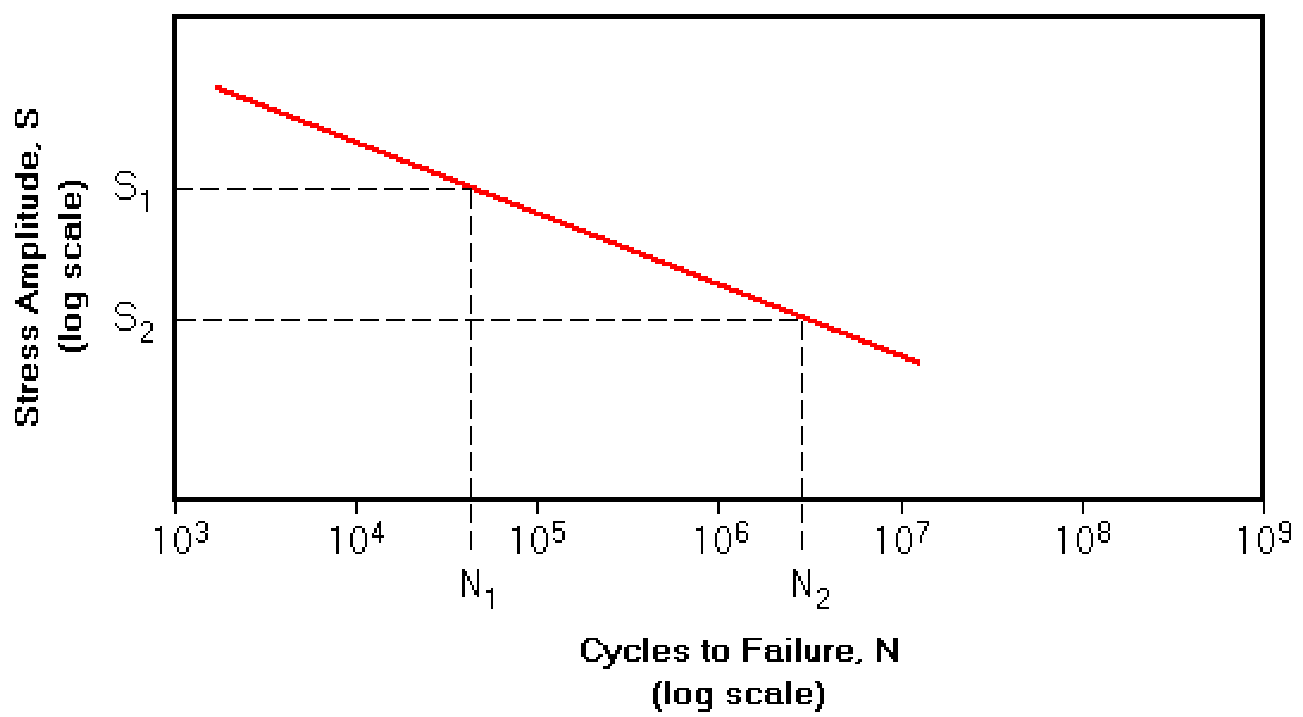
\includegraphics[width=0.7\textwidth]{figures//basquin.png} 
	\caption{Idealized S-N curve for high cycle fatigue.}
	\label{fig.basquin}
\end{figure}
figsn.png
Certain materials have a fatigue limit or endurance limit which represents a stress level below
which the material does not fail and can be cycled infinitely. If the applied stress level is below
the endurance limit of the material, the structure is said to have an infinite life. This is
characteristic of steel and titanium in benign environmental conditions. A typical S-N curve
corresponding to this type of material is shown in \figref{fig.basquin}.

Many non-ferrous metals and alloys, such as aluminum, magnesium, and copper alloys, do not
exhibit well-defined endurance limits. These materials instead display a continuously
decreasing S-N response. In such cases a fatigue strength $S_f$ for
a given number of cycles must be specified. An effective endurance limit for these materials is
sometimes defined as the stress that causes failure at $1x10^8$ or $5x10^8$ loading cycles.

The concept of an endurance limit is used in infinite-life or safe stress designs. It is due to
interstitial elements (such as carbon or nitrogen in iron) that pin dislocations, thus preventing
the slip mechanism that leads to the formation of microcracks. Care must be taken when
using an endurance limit in design applications because it can disappear due to:

\vspace{6pt}
$\bullet$ Periodic overloads (unpin dislocations)

$\bullet$ Corrosive environments (due to fatigue corrosion interaction)

$\bullet$ High temperatures (mobilize dislocations)
\vspace{6pt}     

The endurance limit by itself is not a true property of a material, since other significant influences such
as surface finish cannot be entirely eliminated. However, a test values ($S_e'$) obtained from
polished specimens provide a baseline to which other factors can be applied. Influences that
can affect the endurance limit include:

\vspace{6pt}
$\bullet$ Surface Finish

$\bullet$ Temperature

$\bullet$ Stress Concentration

$\bullet$ Notch Sensitivity

$\bullet$ Size

$\bullet$ Environment

$\bullet$ Reliability
\vspace{6pt}         

\textbf{Power Relationship}   

When plotted on a log-log scale, an S-N curve can be approximated by a straight line as shown
in \figref{fig.basquin}. Basquin’s equation is a power law relationship as  Eq.\ref{eq.basquin} which describes the linear relationship between the applied stress cycles (S) in the y-axis and the number of cycles to failure in the x-axis plotted on a log-log scale.
\begin{equation}
N=BS^\frac{1}{b}
\label{eq.basquin}
\end{equation}
To calculate the slope of the Basquin equation from two significant curve points, we need to solve the system of equations:
$$N_1=N_2\left(\dfrac{S_1}{S_2}\right)^\frac{1}{b},$$
$$b=\dfrac{logS_1-logS_2}{logN_1-logN_2},$$
where $b$ is the slope of the line.
$$B=N_1S_1^{-\frac{1}{b}}=N_2S_2^{-\frac{1}{b}}.$$
For the constant B, in industry  the stress range value (from the maximum cyclic stress to the minimum cyclic stress) is often considered. If the stress values of the S-N curve are given as alternating stresses (which is the common practice), multiply these stresses by 2 to calculate the constant B (stress range = 2* alternating stress, assuming a zero mean stress and full reversal of the cyclic load). If the S-N curve data are given in stress range values, apply them directly in the equation for estimating the constant B. 

The power relationship is only valid for fatigue lives that are on the design line. For ferrous metals this range is from $1\times10^3$ to $1\times10^6$ cycles. For non-ferrous metals, this range is from
$1\times10^3$ to $5\times10^8$ cycles. 

Basquin curves are quite simple but how can we apply them to more complex loadings?

\textit{This limitation is at the origin of the development of more detailed criteria to be described in the next section.}

\section{Basic fatigue criteria }
This bibliographic chapter reviews different methods to calculate the lifetime of multiaxial high cycle fatigue. In fact, the equivalent stress of multiaxial loading and variable amplitude loading reveals the necessity of study these methods. These criteria allows to determine whether the stress trajectory in the stress space leads to the failure of the points concerned.

Papadopoulos suggested, in particular, to group families of fatigue criteria into four categories:
\begin{itemize}
	\item Criteria based on strain
	\item Criteria based on stress
	\item Criteria based on energy
	\item Criteria based on plasticity-damage coupling
\end{itemize}
Generally, the criteria developed in strain(and sometimes in energy) are adapted to the oligocyclic fatigue where the tests are often carried out with imposed strain. Approaches in stress(and sometimes in energy), as well as those based on the coupling plasticity and damage(which have begun to emerge in recent years) are being applied in the domain of endurance. In particular, we will focus on the last three categories and analyze the different approaches.

\subsection{Criteria based on stress}
\vspace{6pt}

Three types of approach can be distinguished:
\begin{itemize}
	\item Critical Plan Approaches
	\item Approaches based on stress invariants
	\item The criteria based on mean stress in an elementary volume
\end{itemize}
For simplicity and to avoid too costly identification procedures of fatigue data, criteria are often expressed using two
parameters. The first relates generally to a shear stress (on a plane or on average over an elementary volume) while
the second reflects the normal stress effects (mean and amplitude) through the hydrostatic stress or the normal stress.
The criteria using the hydrostatic stress are the most numerous (\cite{crossland1956effect}, \cite{sines1959behavior}, \cite{FFE:FFE452}, \cite{thu2008effet}). The micro-macro approach applied to the field of endurance was born with the work of (\cite{van1973khmu}), and since it has been used many times, including by (\cite{papadopoulos1993fatigue}) to take better account of loading path effects.


Many fatigue limit criteria can be written as:
\begin{equation}
f(\tau)+g(\sigma) \leqslant 0
\label{eq.generalfatigue}
\end{equation}
where f and g are given functions of the shear stress τ and of the normal stress σ respectively, as applied to different interfaces within the material.  

The normal and shear stress acting on the material planes and used in Eq.\eqref{eq.generalfatigue} is sometimes defined from a critical plane (\cite{findley1959behavior}), or
through integration at every plane of an elementary volume (\cite{liu1993berechnung}). \cite{thu2008effet} proposes, in
particular, a probabilistic approach based on this type of integration.

\textbf{Crossland Criterion}

In several industries, the required design lifetime of many components often exceeds $ 10^8 $ cycles. This requirement is applicable to aircraft (gas turbine disks $ 10^{10} $ cycles), automobiles (car engine $ 10^8 $ cycles), and railways (high speed train $ 10^9 $ cycles). Although a large amount of fatigue data has been published in the form of S-N (where S is stress and N cycles numbers) curves, the data in the literature has been usually limited to fatigue lives up to $ 10^7 $ cycles (\cite{wachtman2009mechanical}). Using traditional fatigue criteria, a near hyperbolic relationship between stress and fatigue life is assumed, with an asymptotic limit defined as the endurance stress. To predict this asymptotic limit, the Crossland Criterion is probably the most widely known. Crossland proposed that the second invariant of the deviatoric stress tensor and the hydrostatic pressure are the variables governing the endurance limit. 

The classical Crossland criterion defines the fatigue limit of metallic specimens subjected to multi-axial in-phase cyclic stress (\cite{crossland1956effect}) : 
\begin{equation}f(\sqrt{J_{2,a}},P_{max})=\tau_{eq}+aP_{max}-b\leqslant 0\end{equation}

where $\tau_{eq}=\sqrt{J_{2,a}}$ measures  the amplitude of variation of the second invariant of the deviatoric stress  and $P_{max}$ is the maximum hydrostatic stress observed during a loading cycle. If $f(\sqrt{J_{2,a}},P_{max})$ is negative or null, there is no damage. If $f(\sqrt{J_{2,a}},P_{max})$ is positive, there is likely to be damage and hence limited endurance. The physical constants $a$ and $b$ are material's constants that needs to be determined experimentally. The amplitude of the square root of the second invariant of the stress deviator can be defined, in general case, as the half-length of the longest chord of the deviatoric stress path (\cite{Papadopoulos1997219}):
\begin{equation}\sqrt{J_{2,a}}=\frac{1}{\sqrt{2}}\min \limits_{\uline{\uline{S_1}}}\left\lbrace \max \limits_{t}\left( (\uline{\uline{S}}(t)-\uline{\uline{S_1}}):(\uline{\uline{S}}(t)-\uline{\uline{S_1}})\right)\right\rbrace .\end{equation}

Recall that the deviatoric stress $\uline{\uline{S}}$ associated to a stress tensor $\uline{\uline{\sigma}}$  is defined by
\begin{equation} \uline{\uline{S}}=\uline{\uline{\sigma}}-\frac{1}{3}tr\uline{\uline{\sigma}}.
\end{equation}

The maximum value that the hydrostatic stress reaches during the loading cycle is on the other hand:
\begin{equation}
P_{max}=\max\limits_{t}\{\frac{1}{3}tr(\uline{\uline{\sigma(t)}})\}.
\end{equation}

For a proportional cyclic loading, if one introduces the two extreme stress tensors $\uline{\uline{\sigma^A}}$ and $\uline{\uline{\sigma^B}}$ observed during the loading path, together with the stress amplitude
\begin{equation}\uline{\uline{\Delta\sigma}}=\uline{\uline{\sigma^B}}-\uline{\uline{\sigma^A}}\end{equation}
and its deviatoric part $\uline{\uline{\Delta s}} $, the variation of
the second invariant of the stress deviator reduces to 
\begin{equation}
		\begin{split}
			\sqrt{J_{2,a}}&=\frac{1}{2\sqrt{2}}\max\limits_{t}\sqrt{\uline{\uline{\Delta s}}:\uline{\uline{\Delta s}}}\\&=\frac{1}{2\sqrt{2}}\max\limits_{t}\sqrt{(\Delta s_{11}^2+\Delta s_{22}^2+\Delta s_{33}^2+2\Delta s_{12}^2+2\Delta s_{13}^2+2\Delta s_{23}^2)}.
			\end{split}
	\end{equation}

The physical constants $a$ and $b$ can be related to  the limit $t_{-1}$ of endurance in alternate pure shear with $$P_{max}=0, \quad \uuline{\Delta s}=	\left(
\begin{array}{ccc}
0 & 2t & 0\\
2t & 0 & 0\\ 
0 & 0 & 0\\
\end{array}\right)  $$  
and to the limit $f_{-1}$ of endurance in alternate pure traction and compression where there is
$$P_{max}=\frac{1}{3}f, \quad \uuline{\Delta s}=	\left(
\begin{array}{ccc}
\frac{4}{3}f & 0 & 0\\
0 & -\frac{2}{3}f & 0\\ 
0 & 0 & -\frac{2}{3}f\\
\end{array}\right)  $$  
by
\begin{equation}
a=\frac{(t_{-1}-\frac{f_{-1}}{\sqrt{3}})}{\frac{f_{-1}}{3}}, \quad 
b=t_{-1}.
\label{eq.ab}
\end{equation}

Thus the classical Crossland criterion can be written as:
\begin{equation}
\sqrt{J_{2,a}}+a{P_{max}}-b\leqslant 0 .
\end{equation}
with $a$ and $b$ given by Eq.\eqref{eq.ab}.

\textbf{Dang Van Criterion}

In multiaxial fatigue with large number of cycles, the important role of local plasticity on the appearance of a fatigue limit is widely accepted and fully justifies the use of a multi-scale approach. Among the existing approaches, one of the most known and used is that of \cite{van1999introduction}. This criterion is used in particular in the design of certain automotive structures at PSA and
Renault. The criterion (\cite{van1986criterion}) belongs to the family of critical plane type approaches. The main physical
basis of this criterion focuses on the theory of elastic adaptation at two scales, mesoscopic and macroscopic. The macroscopic behavior of the material often remains elastic, only a grain oriented unfavorably undergo
plastic deformation. The author states the following hypothesis: `` The
multiscale approach is settled on the assumption that under high cycle fatigue loading, a structure
will not be fractured by fatigue if an elastic shakedown is reached at the macroscopic scale as well
as at mesoscopic scale " (\cite{van1999introduction}). The approach developed first is
to describe the plasticity across the grain, assuming a yield criterion. The yield criterion is the law of Schmid with a
linear isotropic hardening. The author then search the elastic adaptation(\figref{figDV}) formula and defines a fatigue
test locally ($\Delta$ represents the tensor defining the orientation of the sliding system, $\gamma$ is the plastic slip  and $\tau$
is the amplitude of shear stress on the defined plan).
\begin{figure}[!h]
	\centering
	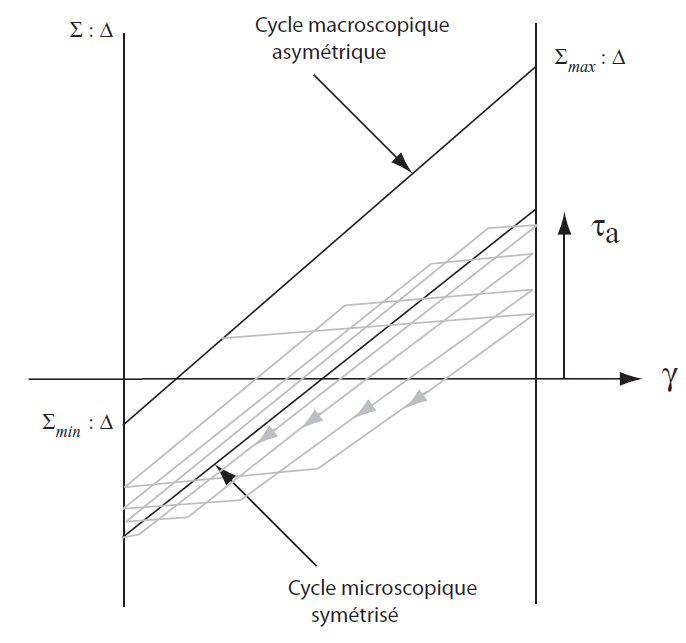
\includegraphics[width=0.7\textwidth]{figures//DV.png} 
	\caption{Elastic adaptation at the two scales(\cite{van1999introduction})}
	\label{figDV}
\end{figure}
Finally, a micro to macro upscaling strategy is applied to determine the criteria on the macroscopic scale. The localization law which is used is Lin-Taylor model that assumes equality of deformations at two scales. Using empirical relationships, the harmful role of the mean stress on the fatigue strength of the material is shown for type of uniaxial tensile stress. Dang Van shows the effect of the mean stress with  hydrostatic stress term in the criteria expressed as a linear combination of mesoscopic  shear stress on the maximum shear plane $\tau_a$ and the hydrostatic stress $\Sigma_h$.


The resulting Dang Van criterion presented in \cite{ballard1995high} is expressed as:
\begin{equation}
\max \limits_{\vec{n}}\left\lbrace \max \limits_{t}\left\{\tau_a{(\vec{n},t)}+a_D\Sigma_h(t)\right\}\right\rbrace \leqslant b_D.
\label{dv}
\end{equation}

where $\tau_a$ denotes the mesoscopic shear stress amplitude and is obtained from a mesoscopic stress tensor $\hat{\bm{\sigma}}$ defined by:
$$\hat{\bm{\sigma}}(t)=(\bm{\sigma}(t)-s^\star).$$
Here $s^\star$ is the center of the smallest hypersphere circumscribed to the loading path in deviatoric stress space. It is obtained by solving a ``min-max" problem as follows:
$$s^\star = arg \min\limits_{s_1}\left\{\max\limits_t\parallel s(t)-s_1\parallel\right\}.$$
In the case of fully reversed loading, the values $s^\star=0$ can be directly deduced without solving the ``min-max problem" as in general case.

The principal stress values of stress tensor $\hat{\sigma}$ being denoted by $\hat{\sigma}_{\Rmnum{3}}(t)\leqslant\hat{\sigma}_{\Rmnum{2}}(t)\leqslant\hat{\sigma}_{\Rmnum{1}}(t)$, one gets the amplitude of shear stress by:
$$\max \limits_{\vec{n}}\tau_a(t)=\frac{1}{2}(\hat{\sigma}_{\Rmnum{1}}(t)-\hat{\sigma}_{\Rmnum{3}}(t)).$$
Here $\Sigma_h(t)$is the hydrostatic stress as a function of the time, given by:$$\Sigma_h(t)=\frac{\sigma_{kk}(t)}{3}.$$
The Dang Van criteria then writes 
\begin{equation}
\frac{1}{2}\left( \hat{\sigma}_{\Rmnum{1}}(t)-\hat{\sigma}_{\Rmnum{3}}(t)\right) +a_D\dfrac{tr\left( \uline{\uline{\sigma}}\right) }{3}\leqslant b_D.
\end{equation}
The material characteristic parameters $a_D$ and $b_D$ of the Dang Van
criterion, can be related to the fully reversed bending (or tension-
compression because of the same stress state between them)fatigue limit, denoted by $f_{-1}$ (or $S_{-1}$), and to the torsion fatigue limit, denoted by $t_{-1}$,

$$a_D=\frac{3t_{-1}}{s_{-1}}-\frac{3}{2};$$  $$b_D=t_{-1}.$$

In the particular case of the uniaxial tension with average load $\Sigma_{xx,m}$ and amplitude $\Sigma_{xx,a}$, the criterion is written as:
$$\Sigma_{xx,a}\left(\dfrac{1}{2}+\dfrac{a_D}{3} \right)+\Sigma_{xx,m}\left(\dfrac{a_D}{3} \right) =b_D.$$

\textbf{Papadopoulos Criterion}

The approach proposed by \cite{papadopoulos1993fatigue} also uses the concept of elastic adaptation and even the localization law. According to him, ``the observations at the mesoscopic scale show that the initiation of a fatigue crack is
defined as the occurrence of micro-cracks corresponding to the rupture of the most deformed crystal grains in an
aggregate. Thus, a fatigue limit criterion can be modeled by a limit value of the accumulated plastic strain in the
most distorted grain."
$$\gamma_{cum}\leqslant\gamma_\infty.$$
He proposes to opt for a mean value of the accumulated plastic strain on all possible slip systems of representative elementary volume(REV). So he chose to use a average value  of accumulated plastic deformation rather than looking at failure of a single crystal. A spherical coordinate system(\figref{fig50}) to guide the vector of normal in material plane, and the unit direction vector $r$ linked to a sliding direction of this plan is used to conduct the integration over all possible orientations.

\begin{figure}[h!]
	\centering
	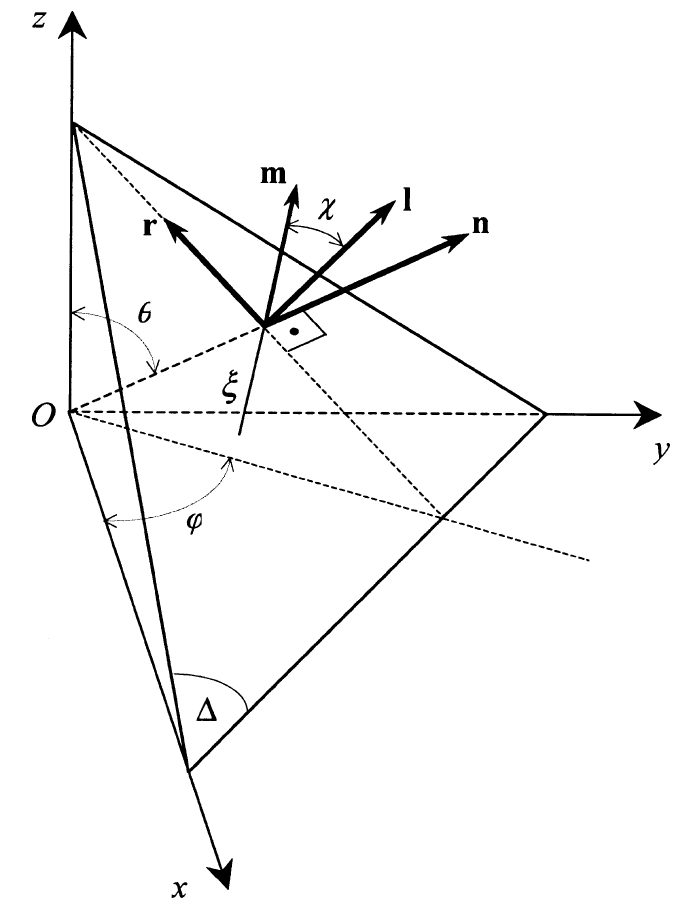
\includegraphics[width=0.5\textwidth]{figures//demopp.png} 
	\caption{Material plane $\Delta$ passing through point O of a body and its
		associated (n, l, r) frame(\cite{papadopoulos1993fatigue}).}
	\label{fig50}
\end{figure}
More precisely, at any point $O$ of a body, a material plane $\Delta$ can be defined by its unit normal vector $\bf n$. This vector
$\bf n$ makes an angle $\theta$ with the z-axis of a $Oxyz$ frame attached to the body, and its projection on the $xy$ plane
makes an angle $\varphi$ with axis $x$. For each plane $\Delta$ a new quantity is introduced called $generalised$ $shear$ $stress$ amplitude and denoted as $T_a$.This shear stress quantity was first introduced in \cite{papadopoulos2001long}
and was subsequently used by other researchers.The critical plane according to our proposal is that onto which $T_a(\varphi,\theta)$ achieves its maximum value. The fatigue limit criterion is written as:
\begin{equation}
max T_a+\alpha_\infty \Sigma_{h,max}\leqslant \gamma_\infty
\end{equation}
where $\alpha_\infty$ and $\gamma_\infty$ are material parameters to be determined (\cite{papadopoulos2001long}), and where we take
$$\Sigma_{h,max}=\max\limits_{t}\left\lbrace \frac{1}{3}tr(\uline{\uline{\sigma}}(t))\right\rbrace $$
He introduced the resolved shear stress $\tau$:
\begin{equation}
\begin{split}
\tau=&[sin\theta cos\varphi\sigma_{xx}+sin\theta sin\varphi\sigma_{xy}+cos\theta\sigma_{xz}](-sin\varphi cos\chi-cos\theta cos\varphi sin\chi)+\\&[sin\theta cos\varphi\sigma_{xy}+sin\theta sin\varphi\sigma_{yy}+cos\theta\sigma_{yz}](cos\varphi cos\chi-cos\theta sin\varphi sin\chi)+\\&[sin\theta cos\varphi\sigma_{xz}+sin\theta sin\varphi\sigma_{yz}+cos\theta\sigma_{zz}]sin\theta sin\chi .
\end{split} 
\label{eqres}
\end{equation}
It is clear that the resolved shear stress is a function of
$\varphi$, $\theta$, $\chi$ and of time $t$ in the case of variable loading, i.e. $\tau=\tau(\varphi, \theta, \chi, t)$. Upon fixing a couple $(\varphi, \theta)$ (i.e. a plane
$\Delta$) and an angle $\chi$ (i.e. a line $\xi$ on $\Delta$), one can define the amplitude of the resolved shear stress $\tau_a$, acting on $\Delta$
along $\xi$ by the formula:
\begin{equation}
\tau_a(\varphi,\theta,\chi)=\frac{1}{2}\big[\max \limits_{t\in P}\tau_a(\varphi,\theta,\chi ,t)-\min \limits_{t\in P}\tau_a(\varphi,\theta,\chi ,t)\big].
\end{equation}
Finally, for a given plane $\Delta$, i.e. for a fixed couple ($\varphi$, $\theta$),
the generalized shear stress amplitude $T_a$ is defined as:
\begin{equation}
T_a(\varphi,\theta)=\sqrt{\frac{1}{\pi}\int_{x=0}^{\frac{\pi}{2}} \tau_a^2(\varphi,\theta,\chi)d\chi}
\label{Ta}
\end{equation}
We note the fatigue limit in fully reversed torsion $t_{-1}$ and the fatigue limit in fully reversed bending $f_{-1}$. From these two tests we get the parameters:
$$\gamma_\infty=t_{-1},$$ 
$$\alpha_\infty=3\left( \frac{t_{-1}}{f_{-1}}-\frac{1}{2}\right) .$$
The Papadopoulos fatigue limit criterion achieves the form (\cite{papadopoulos2001long}):
\begin{equation}
maxT_a+3\left( \frac{t_{-1}}{f_{-1}}-\frac{1}{2}\right) \Sigma_{h,max}\leqslant t_{-1}.
\label{eq:papadopoulos}
\end{equation}
In the particular case of the fully reversed uniaxial tension, the criterion is written as (\cite{papadopoulos2001long}):
$$\dfrac{\Sigma_{xx,a}}{2}+\alpha_\infty\dfrac{\Sigma_{xx,m}}{3} \leqslant\gamma_\infty$$
\textit{These criteria are all based on the notion of cyclic loading, which can be a limitation in general case.}
\subsection{Criteria based on energy}
Depending on the type of density of deformation energy considered per cycle, the
Energy criteria are divided into three groups (\cite{macha1999energy}):
\begin{itemize}
	\item  criteria based on elastic energy
	\item  criteria based on plastic energy
	\item  criteria based on the sum of elastic and plastic energies.
\end{itemize}

The criteria based on the elastic deformation energy can be used in fatigue with a large number of cycles, whereas those based on the plastic deformation energy are more suitable for oligocyclic fatigue.

\cite{ellyin1974criterion} is one of the first to propose a fatigue criterion based on cyclic shear deformation energy. This approach was taken up and complemented by \cite{lefebvre1981cognitive} and \cite{ellyin1991phase} for the case of multiaxial loadings. In France, this approach is reflected in the work of \cite{Froustey1992} and then in \cite{palin1996fatigue} and \cite{banvillet2001prevision}.

\subsubsection{Energy dissipation based on strain energy density}

In their fatigue criterion, \cite{Froustey1992}  have considered a complete cycle of
stresses. They use the mean value on one cycle of
the volumic density of the elastic strain energy, $W_a$, whatever the point
M in the mechanical part.

$$W_a(M)=\frac{1}{T}\int_{0}^{T}\frac{1}{2}\sigma_{ij}(M,t)\varepsilon_{ij}^e(M,t)dt$$

where $\sigma_{ij}(M,t)$ and $\varepsilon_{ij}^e(M,t)$ are respectively the tensor of stresses and the tensor of
elastic strains at the considered point $M$ function of time $t$.Usually the endurance limit
is low enough to consider that the material remains elastic at the macroscopic scale
(\cite{chaboche1988non}). Thus, $W_a$ can be considered as the mean value on one
cycle of the total strain energy density at the considered point.

In 1998 Thierry PALIN-LUC and Serge LASSERRE (\cite{palin1998energy}) proposed a failure criterion based on $W_a$. Their studies show that another limit, called $\sigma^*$, can be defined below
the usual endurance limit of the material, $\sigma_D$. At a considered point a stress amplitude
below this new limit does not initiate observable damage at the microscopic scale (no
micro-cracks). Two static characteristics of the material are necessary: $E$ and $\nu$. Three
experimental endurance limits under fully reversed loadings are needed: the endurance
limit in traction,$\sigma_{Trac,-1}^D$, the endurance limit in rotative bending, $\sigma_{RotBend,-1}^D$, and the
endurance limit in torsion, $\tau_{To,-1}^D$. 

This stress limit $\sigma^*$ can be estimated from
fatigue test results in fully reversed tension and in rotating
bending

$$\sigma^*=\sqrt{2(\sigma_{Trac,-1}^D)^2-(\sigma_{RotBend,-1}^D)^2}.$$

From $\sigma^*$ and by analogy with a sinusoidal traction load the corresponding mean value
of the strain energy volumetric density, $W_{a^*}$, can be calculated , where E is the
Young modulus of the material.

$$W_{a^*}=\frac{\sigma^{*2}}{4E}.$$

Around each point it is always possible to define
the volume $V^* (C_i)$ by the set of points M where $W_a (M)$ is higher than $W_{a^*} (C_i)$
. They postulate that the part of $W_a (M)$ exceeding $W_{a^*} (C_i)$ is the damaging part
of the strain energy volumetric density. They thus calculate $\overline{\omega}_a(C_i)$ 
the volumetric mean value of the strain energy around the critical point $C_i$

$$V^*(C_i)=\lbrace points\; M(x,y,z) \;around\; C_i \;such\; that \;W_a(M)\geqslant W_{a^*}(C_i) \rbrace$$

$$\overline{\omega}_a(C_i)=\frac{1}{V^*(C_i)}\int\int\int_{V^*(C_i)}^{}[W_a(x,y,z)-W_{a^*}(C_i)]d\nu$$

At the endurance limit and at the critical point $C_i$, this new quantity $\overline{\omega}_a(C_i)$ is
supposed to be constant, whatever the uniaxial stress state. If we note $\overline{\omega}_a^D(Uniax)$ its
value at the endurance limit for any uniaxial stress state our criterion can be written by
Eq.\ref{eq.palinfailure}. Failure occurs if this equation is not verified.
\begin{equation}
\overline{\omega}_a(C_i)\leqslant\overline{\omega}_a^D(Uniax).
\label{eq.palinfailure}
\end{equation}

\textit{The limitation of this criteria is that it only deals with constant amplitude load case.}

\subsubsection{A critical plane approach based on energy concepts}


\cite{lagoda1999critical} proposed that under multiaxial loadings the normal strain energy density in the critical plane (i.e. the plane of the maximum damage) to be the energy parameter and translated into deformation or stress amplitude in a given experimental fatigue curve. The history of strain energy density is schematized with use of the rain-flow algorithm. %(\cite{\label{sec:5.1}})
Fatigue damage is accumulated according to Palmgren-Miner hypothesis and endurance limit uses the standard fatigue characteristic of the material, rescaled with use of the considered energy parameter. 
\begin{equation}W(t)=\frac{1}{2}\sigma(t)\varepsilon(t)sgn[\sigma(t),\varepsilon(t)]\label{eq.lagodaWt}
\end{equation}
$$sgn(x,y)=\frac{sgn(x)+sgn(y)}{2}$$

$sgn(x),sgn(y)=0,1,-1$ for distinguishing positive and negative works in a
fatigue cycle. Thus, it allows
to distinguish energy (specific work) for tension and
energy (specific work) for compression. 

If the stress and strain reach their maximum values,
$\sigma_a$ and $\varepsilon_a$, then the maximum energy density value is
\begin{equation}
W_a=\frac{1}{2}\sigma_a\varepsilon_a
\label{eq.lagodaWa}
\end{equation}

Assuming $W(t)$ as the fatigue damage parameter accord-
ing to Eq. \ref{eq.lagodaWt}, we can rescale the standard character-
istics of cyclic fatigue ($\sigma_a-N_F$) and ($\varepsilon_a-N_F$) and obtain a new one, ($W_a-N_F$ ). In the case of high-cycle fatigue, when the characteristic curve ($\sigma_a-N_F$) is used in order to predict the number of cycles $N_F$ to failure, the axis $\sigma_a$ should be replaced by $W_a$, where $W_a$ and $\sigma_a$ are related by:

$$W_a=\frac{\sigma_a^2}{2E}.$$

In the case of low and high-cycle fatigue, when the
characteristic ($\varepsilon_a-N_F$) is used, we can do similar rescaling. 
%We assume $$\sigma_a=\sigma_f'(2N_F)^b$$
%
%From Manson-Coffin-Basquin equation  and Eq.\ref{eq.lagodaWa} we obtain
%
%$$\varepsilon_a=\varepsilon_a^e+\varepsilon_a^p=\frac{\sigma_f'}{E}(2N_F)^b+\varepsilon_f'(2N_F)^c$$
%$$W_a=\frac{1}{2}\sigma_a\varepsilon_a=\frac{\sigma_a}{2}\left[\frac{\sigma_f'}{E}(2N_F)^b+\varepsilon_f'(2N_F)^c\right]=\frac{(\sigma_f')^2}{2E}(2N_F)^{2b}+0.5\varepsilon_f'\sigma_f'(2N_F)^{b+c}$$
%
%Fatigue characteristic for high-cycle fatigue
%takes the form
%$$W_a=\frac{(\sigma_f')^2}{2E}(2N_F)^{2b}$$

The full approach is described in \figref{fig.algorithm}. Having tensors of strain and stress histories we can
determine courses of normal strain energy density (stage
3) in all the planes according to Eq. \ref{eq.lagodaWt} with the distinguished direction $\bar{\eta}$.
\begin{equation}
W_{\eta}(t)=0.25\varepsilon_\eta(t)\sigma_\eta(t)[sgn\varepsilon_\eta(t)+sgn\sigma_\eta(t)]
\label{eq.lagodaWeta}
\end{equation}
where
\begin{equation}
\sigma_\eta(t)=[\hat{l}^2_\eta\sigma_{xx}(t)+\hat{m}^2_\eta\sigma_{yy}(t)],
\label{eq.lagodasigeta}
\end{equation}
\begin{equation}\varepsilon_\eta(t)=[\hat{l}^2_\eta\varepsilon_{xx}(t)+\hat{m}^2_\eta\varepsilon_{yy}(t)+\hat{n}^2_\eta\varepsilon_{zz}(t)],\label{eq.lagodavareta}
\end{equation}
with $\hat{l}^2$, $\hat{m}^2$, $\hat{n}^2$ = direction cosines of the unit vector $\bar{\eta}$.

In the plane stress state the normal vector orientation
to the fracture plane may be described with use of one
angle α in relation to the x-axis. Thus, the direction
cosines of the axis $\bar{\eta}$ are:
$\hat{l}_\eta=cos\alpha$, $\hat{m}_\eta=sin\alpha$, $\hat{n}_\eta=0$.
\begin{figure}[h!]
	\centering
	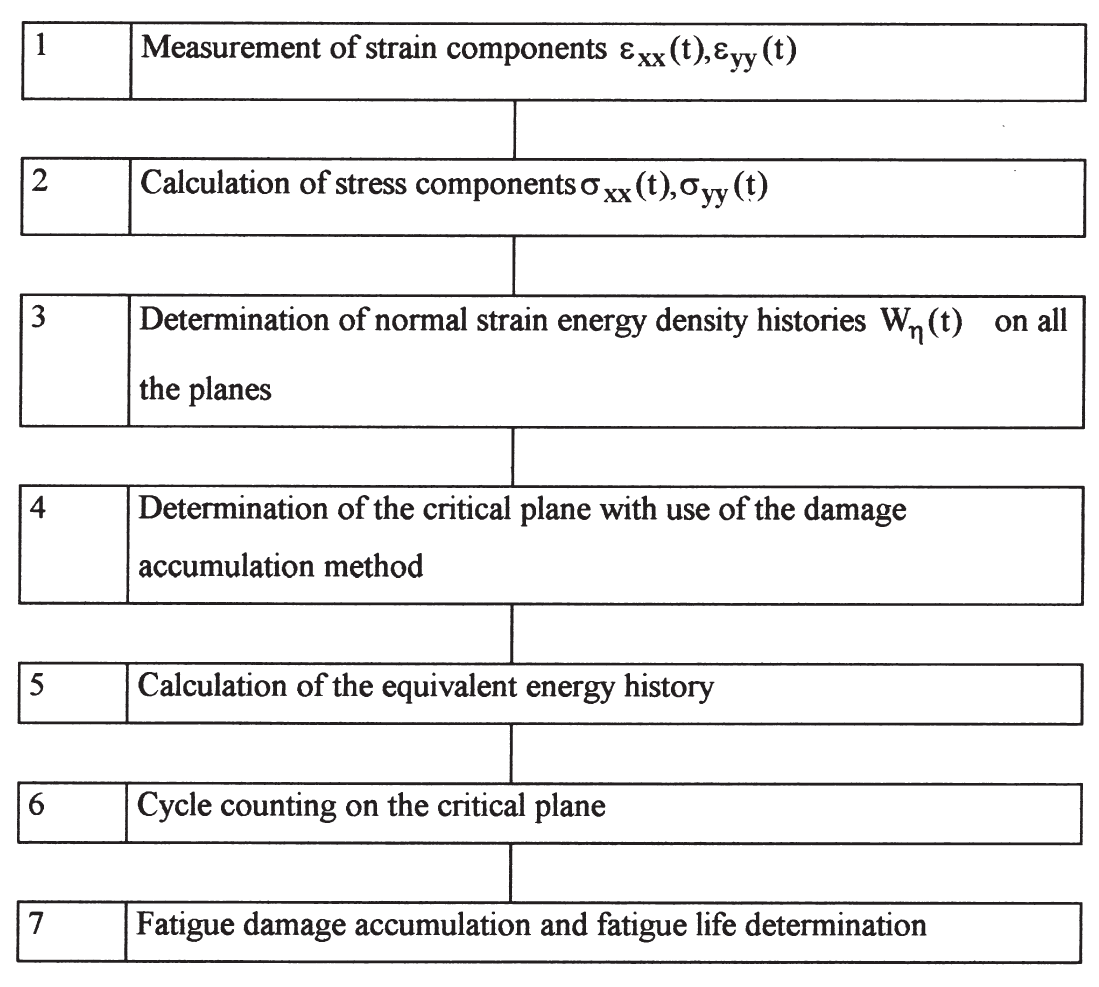
\includegraphics[width=0.7\textwidth]{figures//algorithm.png} 
	\caption{Algorithm of fatigue life determination with use of the energy parameter in the critical plane under biaxial random tension-compression.}
	\label{fig.algorithm}
\end{figure}
In stage 4 the critical plane is determined by $\max \limits_{\eta}\Delta W_{\eta}(t)$ according to
the damage accumulation method Eq.\ref{eq.lagodaWeta}. Fatigue lives
were determined at particular expected planes according
to the following stages. When the energy density history
at the given plane in stage 6 has been determined, the
energy cycles are counted with the rain flow method;
next damage is accumulated according to Palmgren-
Miner hypothesis taking into account energy
cycle of amplitude larger than a $W_{af}$ with $a=\frac{1}{4}$.
$$S(T_0)=\sum_{i=1}^{j}\dfrac{n_i}{N_0(W_{af}/W_{ai})^{m'}} \qquad for \quad W_{ai} \geqslant aW_{af},$$
$$S(T_0)=0 \qquad for \quad W_{ai} \leqslant aW_{af},$$
where $S(T_0)$ is material damage up to time $T_0$ ; $j$ is number of class intervals of the histogram of the amplitudes
of the strain energy density; $W_{af}$ is fatigue limit
expressed by strain energy density;  $m'$ is slope of fatigue curve; $N_0$ is a number of cycles corresponding to the fatigue
limit $W_{af}$ ; $n_i$ is a number of cycles with amplitude $W_{ai}$.

When the degree of damage at observation time $T_0$ is
determined, the fatigue life is calculated by:
$$T_{cal}=\dfrac{T_0}{S(T_0)}.$$

\textit{This method is able to take general loadings, but still requires cycle counting. And the determination of critical plane in multiaxial load is laborious. Also, they use the miner's damage law which can not account for the sequencing effect.}

\subsubsection{Lamefip Criterion}
The so-called Lamefip criterion, presented here with its latest version (\cite{benabes2006approche}), makes it possible to handle all types of loads and to take into account the effect of the stress gradients. This criterion is based on the notion of the volume of influence around the ``critical point" and uses as a parameter the volume density of straining work supplied per cycle to each volume element.

\cite{ellyin2012fatigue} showed that the use of both the plastic and elastic strain work can be used
as damage parameter in multiaxial fatigue. The LAMEFIP criterion (\cite{banvillet2003volumetric}),
devoted to the field of endurance or limited endurance, uses for damage parameter, the volumetric density of the strain work given to the material per loading cycles after elastic shakedown(supposed to be reached after a few thousands cycles ).

The proposal is based on two main hypothesis : (i) the strain work given to the material per loading cycle is considered as the driving force for fatigue crack initiation and (ii) it is calculated after macroscopic elastic shakedown.

Many authors use cycle counting techniques to extract, from a random stress tensor sequence, cycles from which the damage could be estimated. These techniques have two main drawbacks : (i) the choice of the cycle counting algorithm influences the calculated fatigue life since the number of counted cycles is algorithm dependent (\cite{dowling1983fatigue}), and (ii) for multiaxial non-proportional stress states, in many approaches from the literature, the variable chosen for cycle counting differs from the damage parameter. To avoid such drawbacks an incremental model has been developed. The strain work density given at a point M is written in an incremental way as follows :

$$dW_g(M,t)=\sum_{i=1}^{3}\sum_{j=1}^{3}\left\langle \sigma_{ij}\left( M,t\right)\dot{\epsilon}_{ij}\left( M,t \right)\right\rangle  dt .$$

\noindent
- where $\epsilon_{ij}\left( M,t\right)$ are the strain tensor components and $\dot{x}= dx/dt$,\\
- $\sigma_{ij}\left( M,t\right)$ are the stress tensor components,\\
- and $\left\langle m\right\rangle$ gives the positive value of $m$ according to : $\left\langle m\right\rangle=1$ if $m \geqslant 0$; $\left\langle m\right\rangle=0$  if $m < 0$.

As underlined by \cite{ellyin2012fatigue}, the strain work can be calculated as the sum of elastic and plastic strain works, so that :
$$dW_g(M,t)=dW_g^e(M,t)+dW_g^p(M,t).$$
The framework of this study being HCF and MCF, they choose to consider only the elastic part of the strain work (Eq.\eqref{eq.lamefip1}) in the elastic shakedown state. The cumulated strain work on a time
sequence of duration $T$ is equivalent to the integral of $dW_g^e(M,t)$ over $T$ as in Eq.\eqref{eq.lamefip2}. \cite{banvillet2003volumetric} has shown that for an uniaxial stress state $W_g$ is not shape dependent (sinus, triangle,square, etc...).
\begin{equation}
dW_g^e(M,t)=\sum_{i=1}^{3}\sum_{j=1}^{3}\left\langle\sigma_{ij}\left( M,t\right)\dot{\epsilon}_{ij}^e\left( M,t\right)\right\rangle dt .
\label{eq.lamefip1}
\end{equation}
\begin{equation}W_g(M,T)=\int_{t}dW_g(M,t).\label{eq.lamefip2}
\end{equation}

To take into account the material sensitivity to the stress triaxiality, the triaxiality degree at a point M is defined by the ratio of the strain work associated with the spherical part of the stress tensor over the total strain work of \cite{banvillet2003volumetric}, but in an incremental way :
$$dT(M,t)=\dfrac{dW_g^{Sph}(M,t)}{dW_g(M,t)} \qquad if \qquad  dW_g(M,t)\neq0,\ otherwise \quad dT(M,t)=0,$$
with
$$dW_g^{Sph}(M,t)=\dfrac{1}{3}\sum_{k=1}^{3}\sigma_{kk}(M,t)\sum_{l=1}^{3}\dot{\epsilon}_{ll}^e(M,t)H\left( \sum_{k=1}^{3}\sigma_{kk}(M,t)\sum_{l=1}^{3}\dot{\epsilon}_{ll}^e(M,t)\right)dt .$$
The material sensitivity to stress triaxiality is considered by using an empirical function
$F(dT,\beta_m)$ (Eq.\eqref{eq.lamefip3}) depending on the material parameter $\beta_m$ identified from two fully reversed
fatigue limits (rotating bending and torsion). At any instant, for a multiaxial stress state, the
strain work given to the material is corrected to evaluate an uniaxial equivalent strain work
$d{W_f}_{eq} (M,t)$ (Eq.\eqref{eq.lamefip4}):
\begin{equation}
F(dT(M,t),\beta_m)=\dfrac{1}{1-dT(M,t)}\left[ 1-\dfrac{1}{\beta_m}ln\left[1+dT(M,t)(e^{\beta_m}-1) \right] \right] .
\label{eq.lamefip3}
\end{equation}
\begin{equation}
d{W_g}_{eq} (M,t)=d{W_g}(M,t)\dfrac{F(dT_{uniax},\beta_m)}{F(dT(M,t),\beta_m)}.
\label{eq.lamefip4}
\end{equation}
A threshold $W_g^*$ is introduced. It represents the volume density of the minimum elastic deformation work to be provided to create, after a large number of cycles, irreversible damage in a REV. The volume influencing fatigue crack initiation $V^*$ is thus
defined whatever the stress state is at the critical point.
\begin{equation}
W_g^*=W^*_{g,uniax}\dfrac{F(dT_{C_i},\beta_m)}{F(dT(uniax),\beta_m)}.
\label{eq.lamefip5}
\end{equation}
\begin{equation}
V^*(C_i)=\left\lbrace points \; M(x,y,z) \; around \; C_i \; so \; that \; {W_g}_{eq} (M,t)\geqslant W_g^*\right\rbrace .
\label{eq.lamefip6}
\end{equation}

 Assuming that the set of points of the volume of influence plays a significant role in the initiation of a fatigue crack at the critical point $C_i$, the volume mean value of the damaging work provided in the $V^*$ of influence is written:

$${W_g}_{C_i}=\dfrac{1}{V^*(C_i)}\int_{V^*(C_i)}\left[{W_g}_{eq}(M,T)- W_g^*\right] $$

In the case of uniaxial loading, the values of $W_g^*$ are expressed as:
$$W_g^*=\dfrac{2s_{-1}^2-f_{rot-1}^2}{E}$$
$f_{rot-1}$ and $s_{-1}$ denote respectively the endurance limits in alternating rotational bending and traction.
The final criterion proposed by \cite{banvillet2003volumetric} is summarized in the following relation:
$${W_g}_{C_i}<{W_g}_{eq}.$$

Where ${W_g}_{eq}$ Is the permissible limit value of ${W_g}_{C_i}$  at the limit of fatigue.

\textit{This approach is possible to predict the $S–N$ curves from
	a uniaxial one since the proposal is load type and mean
	load sensitive. However, the threshold work is another form of the fatigue limit which can be inaccurate microscopically. In addition, it does not deal with random loading.}

\subsection{Criteria based on plasticity-damage coupling}
In recent years, a new class of criteria coupling mesoplasticity and damage has emerged.  \cite{lemaitre1999two} have, for example, used the approach introduced by \cite{lemaitre1985mecanique} based on the thermodynamics of irreversible processes and the mechanics of continuous media.  \cite{flaceliere2004contribution} also proposed a model based on a plasticity-damage coupling and attempted to account for the phenomena of damage observed experimentally on a C35 steel. In this work, we will focus on a more recent approach proposed by \cite{monchiet2006contributions}.
\subsubsection{Criterion of Monchiet et al}
In order to account for the coupling plasticity-damage in HCF, \cite{monchiet2006contributions} uses a micro-mechanical approach based on the work of  \cite{gurson1977continuum}. The damage is represented by a magnitude $f$ related to the development of porosity in the sliding bands at the origin of the initiation of the fatigue cracks. A yield surface, of the type defined by Gurson, is used:
\begin{equation}
\dfrac{\Sigma_{equ}^2}{\Sigma_0^2}+2fcosh\left(\dfrac{3}{2}\dfrac{\Sigma_h}{\Sigma_0}\right)-1-f^2\leqslant 0 ,
\label{eq.monchiet1}
\end{equation}
where $\Sigma_{equ}$ is the equivalent stress, $\Sigma_h$ The hydrostatic stress and $\Sigma_0$ the elastic limit of the matrix.

Plasticity occurs locally when the equivalent stress reaches the yield limit. The authors take into account two mechanisms of damage in the evolution of the porosity:

\vspace{6pt}
\begin{itemize}
	\item  The first is related to the creation of gaps by annihilation of dislocations. This mechanism is at the origin of the accumulation of point defects of the lacunar or interstitial type along the persistent slip bands (PSB). The phenomenological model proposed by \cite{essmann1979annihilation} gives access to the porosity $f_a$:
	\begin{equation}
	f_a= A_0\left\lbrace k_a\gamma_{cum}-1+exp\left(-k_a\gamma_{cum} \right)  \right\rbrace .
	\label{eq.monchiet2}
	\end{equation}
	
	\item  The second mechanism is related to the growth of micro-cavities. Using an incompressibility hypothesis, $f_g$ is defined by:
	\begin{equation}
	f_g=\left\lbrace 1-exp\left(3\epsilon_h^p \right) \right\rbrace.
	\label{eq.monchiet3}
	\end{equation}
\end{itemize}

It is important to note that the first mechanism involves the accumulated plasticity $\gamma_{cum}$, related to amplitude effects. The second mechanism depends on the hydrostatic plastic deformation $\epsilon_h^p$, and allows the taking into account of the mean stress effects.

The fatigue criterion is established on the basis of the following hypothesis: ``a sufficient condition for nucleation of a fatigue crack is obtained if the porosity reaches a critical value $f_c$".
\begin{equation}
f\left( \gamma_{cum},\epsilon_h^p\right) =f_a+f_g\leqslant f_c.
\label{eq.monchiet4}
\end{equation}

Noting $\gamma_c$, the critical value of the cumulative plasticity for which the fatigue criterion is reached when $\epsilon_h^p=0$, it becomes:
\begin{equation}
f_c=\left\lbrace A_0\left\lbrace k_a\gamma_{c}-1+exp\left(-k_a\gamma_{c} \right)  \right\rbrace \right\rbrace.
\label{eq.monchiet5}
\end{equation}
\begin{equation}
\gamma_{cum}=\uline{\uline{T_a}}:\Delta\uline{\uline{\epsilon}}.
\label{eq.monchiet5.5}
\end{equation}

Where $T_a$ is defined the same as the one used in Papadopoulos criterion as reviewed in Eq.\eqref{Ta}. The use of Eq.\eqref{eq.monchiet4} and Eq.\eqref{eq.monchiet5} leads, for the limiting cases $k_a \gg 1$ to Eq.\eqref{eq.monchiet6}, and for $k_a << 1$ to Eq.\eqref{eq.monchiet7}, when noting $\epsilon_c$ the critical plastic deformation, equal to $f_c / 3$ in the case of $\gamma_{cum} 0$, 

either 
\begin{equation}
\dfrac{\gamma_{cum}}{\gamma_{c}}+\dfrac{\epsilon_h^p}{\epsilon_c}=1, \left( k_a \gg 1\right) 
\label{eq.monchiet6}
\end{equation}

or
\begin{equation}
\left( \dfrac{\gamma_{cum}}{\gamma_{c}}\right) ^2+\dfrac{\epsilon_h^p}{\epsilon_c}=1. \left( k_a \ll 1\right) 
\label{eq.monchiet7}
\end{equation}

The effect of the mean stress is taken into account by the term of hydrostatic deformation. Since $\gamma_{cum}$ and $\epsilon_h^p$ are defined on the grain scale, the macroscopic expression of the criterion requires to link these quantities to the macroscopic magnitudes of the loading.

The next step is to look for elastic adaptation conditions and to apply a micro-macro path. The numerical results obtained make it possible to establish the following relations between the loading parameters and the parameters of the local criterion, where the macroscopic  load surface is then written:
\begin{equation}
F=\left( \dfrac{T_a}{\tau_d}\right) ^2+2f_ccosh\left\lbrace\dfrac{\sqrt{3}}{2}\dfrac{\Sigma_{h,m}}{\tau_h} \right\rbrace-1-f_c^2\leqslant 0.
\label{eq.monchiet8}
\end{equation}
In Eq.\eqref{eq.monchiet8}, $\tau_d$ and $\tau_h$ are the deviatoric and hydrostatic part of the plastic flow threshold associated with an isotropic hardening. $\Sigma_{h,a}$ is the hydrostatic pressure. $T_a$ is accumulated plastic flow.

The isotropic hardening was taken into account by replacing the
$\tau_d$ and $\tau_h$, defined by: $\tau_d = \tau_0 + R_d$ and $\tau_h = \tau_0 + R_h$. The quantities $R_d$ and $R_h$ are the two isotropic hardening variables. 

The hydrostatic pressure is related to the hydrostatic plastic deformation by:
\begin{equation}
\Sigma_{h,m}=-\left( \dfrac{4c}{f_cln(f_c)}\left( 1-f_c\right)+3k^{\ast} \right) \epsilon_h^p.
\label{eq.monchiet9}
\end{equation}



In Eq.\eqref{eq.monchiet9}, $c$ and $k^{\ast}$ are parameters related respectively to the kinematic hardening and to the homogenization scheme.

The implementation of this criterion requires the identification of 12 parameters:
\begin{flushleft}
	\qquad - \qquad two parameters, $\gamma_c$ and $\epsilon_c$ linked to the local criterion.\\
	\qquad - \qquad two parameters, $A_0$ and $k_a$, related to the mechanisms of nucleation of cracks.\\
	\qquad - \qquad three parameters related to hardening, $R_0$ And $\tau_0$ linked to the isotropic hardening, $c$ linked to  the kinematic hardening\\
	\qquad - \qquad two coefficients linked to the homogenization scheme, $\mu$ and $k$.\\
	\qquad - \qquad a cubic anisotropy coefficient of the grain $p_1$\\
	\qquad - \qquad a latent coefficient of strain hardening h\\
	\qquad - \qquad a critical porosity coefficient $f_c$\\
\end{flushleft}

\textit{All of these parameters are microscopic, which poses a problem in their identification. Some elements of this modeling have been taken up by \cite{charkaluk2009revisiting}, \cite{charkaluk2007approche} in dissipative approaches. The limitation of this method is that it still requires cycle counting which in complex load case is not feasible.}

\section{Calculation method without cycle counting}
This part presents the existing method of prediction of lifetime, which does not need the algorithm of cycle counting. These kind of methods are still minority and usually more delicate to implement, but present the advantage of free the choice of variable of counting proved to be ``dangerous''. The method presented here is the morel method which is based on stress.

\subsection{Morel's method}
Morel's method (\cite{Morel2000101}) is based on a mesoscopic approach of critical plane type with the
choice of plastic deformation as mesoscopic cumulative damage variable. The description below is taken from his paper. Multiaxial and variable amplitude loading can be analyzed with this method.
To depict the fatigue crack initiation phenomenon in polycrystalline metallic materials, two scales of description of a material will be distinguished: the usual macroscopic scale and a mesoscopic one. The macroscopic scale is defined with the help of an elementary volume
V determined at any point O of a body as the smallest sample of the material surrounding O that can be considered to be homogeneous. V contains a large number of grains (crystals) and the
mesoscopic scale is defined as a small portion of this
volume. In the high cycle fatigue regime, some grains
undergo local plastic strain while the rest of the matrix
behaves elastically (the overall plastic strain is
negligible).

\begin{flushleft}
	Macroscopic quantities. They are:
	\begin{table}[!h]
		\begin{tabular}{lllll}
			$\uline{\uline{\Sigma}}$ & macroscopic stress tensor &  &  &  \\
			$\uline{\uline{E}}$ & macroscopic strain tensor &  &  &  \\
			${\uline{C}}$ & macroscopic shear stress vector  &  &  &  \\
			${\uline{T}}$ & macroscopic resolved shear stress vector acting on an easy glide direction&  &  &  \\
			$T_a$ & amplitude of the macroscopic resolved shear stress  &  &  &  \\	
			$P$ & macroscopic hydrostatic stress.&  &  &  \\	
		\end{tabular}
	\end{table}
	
	Mesoscopic quantities. They are:
	\begin{table}[!h]
		\begin{tabular}{lllll}
			$\uline{\uline{\sigma}}$& mesoscopic stress tensor &  &  &  \\
			$\uline{\uline{\varepsilon}}$ & mesoscopic strain tensor &  &  &  \\
			$\uline{\tau}$& mesoscopic resolved shear stress vector acting on an easy glide direction &  &  &  \\
			$\gamma^p$& mesoscopic shear plastic strain &  &  &  \\
			$\Gamma$ & accumulated plastic mesostrain &  &  &  \\
			$T_\sigma$ & measure proportional to an upper bound of the plastic mesostrain  &  &  &  \\
			& accumulated on an elementary
			material plane $\Delta$, also average value of $T_a$&  &  &  \\
			$T_\Sigma$ & maximum value of  $T_\sigma$&  &  &  \\
			$H$ & phase-difference coefficient.&  &  &  \\
		\end{tabular}
	\end{table}
\end{flushleft}

\newpage
\textbf{Constant amplitude loading}
\vspace{6pt}

\textbf{Local stress estimation in high cycle fatigue}

By assuming that only one glide system (defined by a normal vector $\uline{n}$ to a plane and a vector
(direction) $\uline{m}$ within this plane) is active for every plastically deforming grain of the metal, \cite{papadopoulos1993fatigue}
established a macro–meso passage for a glide system activated in a flowing crystal:
\begin{equation}
\uline{\tau}=\uline{T}-\mu\gamma^p\uline{m}
\label{macromeso}
\end{equation}
where $\uline{\tau}$ and $\uline{T}$ are the mesoscopic and macroscopic
resolved shear stresses acting along the slip direction $\uline{m}$ and are defined by:
\begin{equation}
\uline{\tau}=(\uline{m}\cdot\uuline{\sigma}\cdot\uline{n})\uline{m}
\label{tau}
\end{equation}
\begin{equation}
\uline{T}=(\uline{m}\cdot\uuline{\Sigma}\cdot\uline{n})\uline{m}
\label{T}
\end{equation}
and $\gamma^p$  is  the magnitude of the plastic mesoscopic shear strain deduced from the plastic flow rule associated to Eq.\ref{Schmid}.
\begin{figure}[h!]
	\centering
	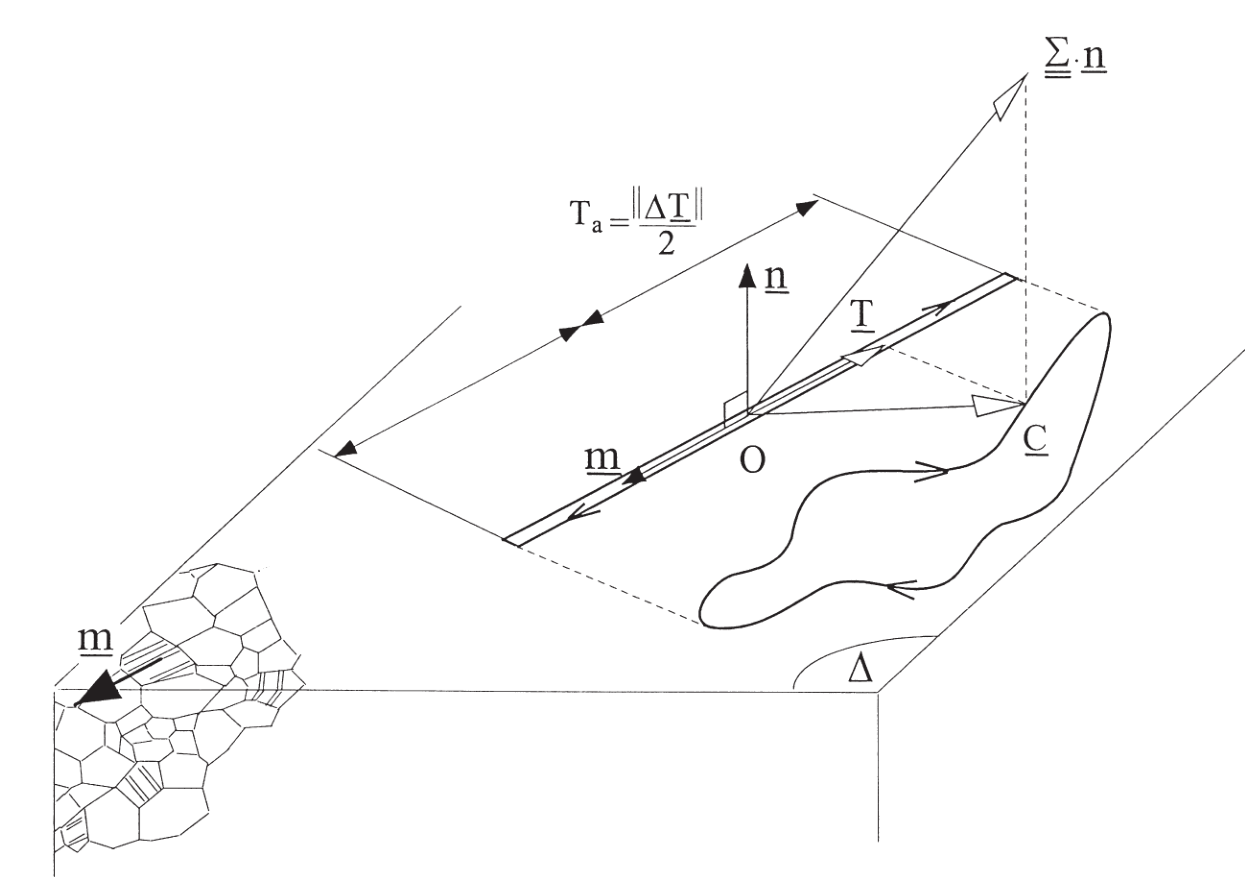
\includegraphics[width=0.8\textwidth]{figures//glid.png} 
	\caption{Path of the macroscopic shear stress $\uline{C}$ acting on a material plane $\Delta$ and the corresponding path of the macroscopic resolved shear stress $\uline{T}$ acting on an easy glide direction (\cite{Morel2000101}).}
	\label{glid}
\end{figure}

\textbf{Initiation of slip in the crystal}

The plasticity criterion is determined by Schmid's law with isotropic and kinematic hardening:
\begin{equation}
f(\uline{\tau},\uline{b},\tau_y)=(\uline{\tau}-\uline{b})\cdot(\uline{\tau}-\uline{b})-\tau_y^2=0
\label{Schmid}
\end{equation}
where $\uline{b}$ is the kinematic back stress, and $\tau_y$ is the yield limit subjected to hardening.

Three successive linear isotropic hardening rules have
been adopted on $\tau_y$ to describe the crystal behavior from
initial yield to failure (\figref{3phases}a). The damage variable is the accumulated plastic mesostrain $\Gamma$ (\figref{3phases}b).
In the first phase, we have a linear increase $\dot{\tau}_y=g\dot{\Gamma}$, in the second phase when $\tau_y$ reaches a saturation $\tau_{lim}$, $\dot{\tau}_y=0$, and then above a certain threshold, we have softening $\dot{\tau}_y=-h\dot{\Gamma}$.

In the description and implementation of his method, the author draws heavily on the work developed by Papadopoulos including the use of a measure of cumulative mesoscopic plastic deformation   and modeling the behavior of grain in three distinct phases (hardening, saturation and softening); he considers the cumulative mesoscopic plastic deformation $\Gamma$ as damage parameter and assumes that the initiation of a fatigue crack occurs when the latter reaches a
critical value $D = D_R = \Gamma_R$ (\figref{3phases}). 
\begin{figure}[h!]
	\centering
	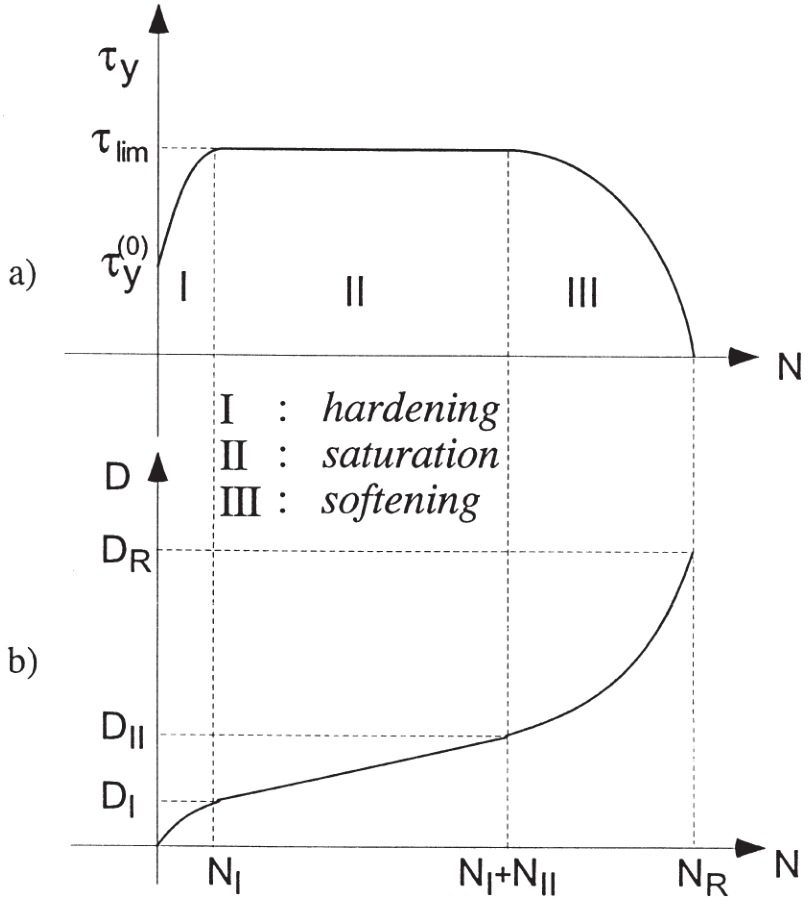
\includegraphics[width=0.5\textwidth]{figures//3phases.png} 
	\caption{(a) Yield limit evolutions and (b) damage evolution in the three behavior phases (hardening, saturation and softening) when a cyclic loading is applied.(\cite{Morel2000101}).}
	\label{3phases}
\end{figure}

\textbf{Loading limit estimation}

The estimation of the yield limit in the saturation phase $\tau_{lim}$ (defining the cyclic behavior of the crystal) is
carried out by the definition of a limit loading, such that:
\begin{equation}
T_{\Sigma lim}+\alpha P_{max lim}=\beta
\end{equation}
\begin{equation}
T_{\Sigma lim}=\frac{-\alpha P_m+\beta}{\alpha+\frac{T_\Sigma}{P_a}}\cdot\frac{T_\Sigma}{P_a},
\label{Tlim}
\end{equation}
where $T_{\Sigma}$ is the maximum value of the macroscopic stress $T_{\sigma}$ and $P_a$ the hydrostatic stress amplitude.
The actual and limit loadings are said to be ``similar''. Let $C_A$ and $\tau_{lim}$ be the amplitudes of the macroscopic
shear stress acting on the critical plane corresponding to
the actual and limit loadings respectively. More precisely, $C_A$ is the length of the longest chord of the load tregectory. $\tau_{lim}$ can be
easily deduced from the relation in the paper (\cite{morel1998fatigue}) between two ‘similar’ loadings (actual
and limit):
$$\dfrac{T_{\Sigma}}{C_A}=\dfrac{T_{\Sigma lim}}{\tau_{lim}}\Rightarrow\tau_{lim}=\dfrac{T_{\Sigma lim}}{H}$$

where H constitutes a ‘phase-difference coefficient’:

\begin{equation}
H=\frac{T_{\Sigma}}{C_A}
\label{eqH}
\end{equation}
It is worth mentioning that the more open the elliptic
path, the higher the coefficient H.  

\begin{figure}[h!]
	\centering
	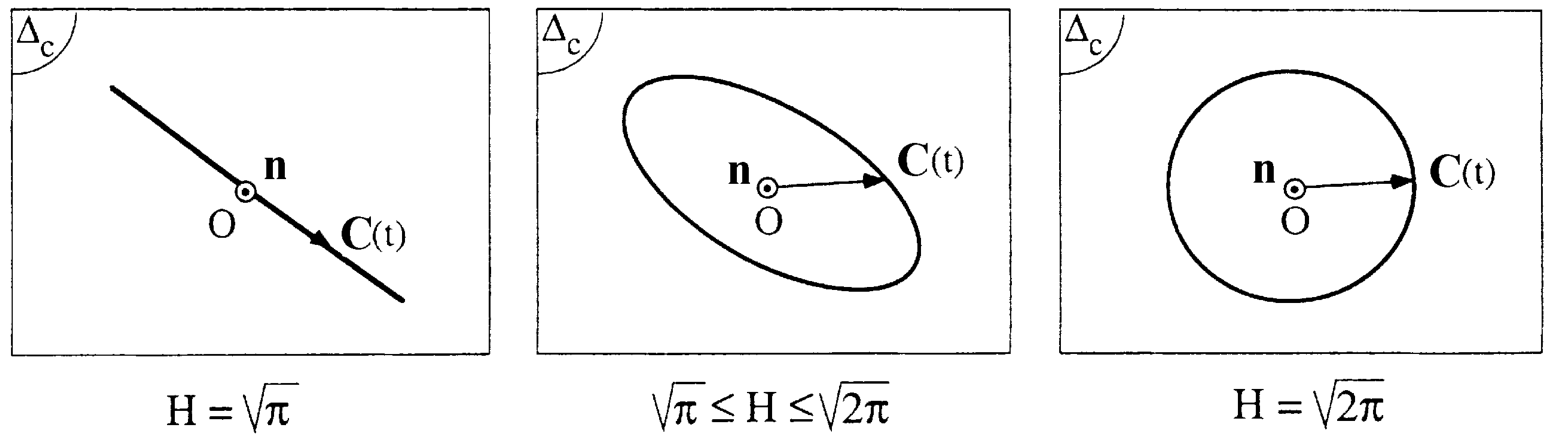
\includegraphics[width=0.9\textwidth]{figures//H.png} 
	\caption{Different paths and corresponding values of the phase-difference coefficient $H$ (\cite{Morel2000101}).}
	\label{figH}
\end{figure}
For a proportional
loading, H is equal to $\sqrt{\pi}$. In the case of a particular
circular path, H reaches the maximum value $\sqrt{2\pi}$(\figref{figH}). 
The linear path and the circular one lead to two bounds of
the coefficient H.

\textbf{Number of cycles to failure}

Once the accumulated plastic mesostrain $\Gamma$ along the particular gliding system reaches a critical value $\Gamma_R$, these grains are said to be broken. An analytical expression of the number
of cycles to initiation (S–N curve) can be achieved:
\begin{equation}
\Gamma=\Gamma_R \, \Rightarrow \, N_i=pln\left(\frac{C_A}{C_A-\tau_{lim}}\right)+q\left(\frac{\tau_{lim}}{C_A-\tau_{lim}}\right)-\frac{r}{C_A}
\label{eq.morelNF}
\end{equation}
where $p$, $q$ and $r$ are functions of the hardening parameters of the three phases defined above.

From Eq.\eqref{Tlim} and Eq.\eqref{eqH} we can find the yield point $\tau_s$ of the crystal in the saturation phase as a function of the amplitude $P_a$ and the mean value $P_m$ of the hydrostatic pressure, the phase difference of coefficient $H$ and two material related parameters $\alpha$ and $\beta$ :
\begin{equation}
\tau_{lim}=\tau_s=\frac{-\alpha P_m+\beta}{\alpha\frac{P_a}{C_A}+H}
\label{taus}
\end{equation}
In the last relation Eq.\ref{eq.morelNF}, the detrimental effect of out-
of-phase loading is introduced through $\tau_{lim}$. As the coefficient H increases, $\tau_{lim}$ as well as $N_i$ decrease and therefore more damage is accumulated. The identification of
the model parameters requires two endurance limits
(parameters a and b of the endurance criterion) and a
single S–N curve (parameters $p$, $q$ and $r$).

\textbf{Damage accumulation}

Damage accumulation calculation is still carried out
by adopting the three successive linear isotropic hardening rules of crystal behaviour (\figref{3phases}). Consequently, the
mechanical parameters used for damage accumulation
are the macroscopic resolved shear stress on a given
gliding system and the hydrostatic stress.

Damage calculation by morel's method for a loading of $N_{(I)}$ cycles of a general loading sequence $\uline{\uline{\Sigma}}(t)_{0\leqslant t\leqslant T(I)}$ is described as follows:

The underlying model is as in Dang Van, or in Papadopoulos: the material behaves plastically at a certain mesoscale, and the damage is related to the plastic deformation observed in the worst slip system characterized by a direction $\uline{m}$ in a plane of normal $\uline{n}$. The meso and macro shear stress
$$T=\uline{m}\cdot \uline{\uline{\Sigma}}\cdot \uline{n} \; and \; \tau=\uline{m}\cdot \uline{\uline{\sigma}}\cdot \uline{n}$$
are related by the Lin Taylor rule
$$\tau=T-\mu\gamma^p$$
with a local plastic slip $\gamma^p$ governed by the plastic flow rule associated to the yield surface
$$(\tau-b)^2-\tau_y\leqslant 0.$$
There is a kinematic hardening(with slope $c$) to govern the evolution of $b$ and an isotropic hardening with saturation to govern the evolution of $\sigma_y$.

In Morel's model as seen above, the fatigue control mechanism is embedded in the construction of the saturation limit $\tau_{lim}$ of $\tau_y$ which is constructed separately on each slip system using fatigue test data. More precisely, we assume that the given material has an endurance limit in uniaxial loading given as in Papadopoulos by
$$\Delta T/2+\alpha P_{max}=\beta$$
with material coefficients $\alpha$ and $\beta$, $\Delta T/2$ the amplitude of the resolved shear stress, and $P_{max}$ the maximum hydrostatic stress. For a given cyclic shear loading on the considered slip line of amplitude $T_a$, average hydrostatic stress $P_m$ and amplitude of hydrostatic stress $P_a$, we introduce the amplitude scaling $k$ where we have
$$kT_a+\alpha\left( kP_a+P_m\right)=\beta  $$
 $$\Rightarrow \; k=\dfrac{\beta-\alpha P_m}{T_a+\alpha P_a}$$ 
 which will send this loading to the endurance curve, and a shape factor $\sqrt{\pi}\leqslant H\leqslant \sqrt{2\pi}$ characterizing the shape of the loading path in the considered plane of normal $\uline{n}$. The local saturation limit $\tau_{lim}(\uline{m},\uline{n})$ is then defined by the amplitude of the shear loading $T_a$ once multiplied by the scaling factor $k$ and corrected by the shape factor $H$, giving
$$\tau_{lim}(\uline{m},\uline{n})=\frac{k}{H}T_a(\uline{m},\uline{n})=\frac{1}{H}\frac{\beta-\alpha P_m}{T_a+\alpha P_a}T_a(\uline{m},\uline{n}).$$
By using the amplitude scaling factor $\tau_{lim}$ becomes resolved shear stress limit which is Papadopoulos fatigue criteria implicit. In this framework, Morel's method uses three successive steps for computing the damage created by the repeated loading sequence:

\begin{enumerate}
\item Find the critical plane $\uline{n}$ maximizing the in plane plastic deformation $\int_{\uline{m}}\gamma^p$ which will be induced by the loading sequence, assuming linear isotropic hardening without saturation.
\item On this plane  $\uline{n}_c$, on each direction $\uline{m}$, compute the plastic history, that is
\begin{enumerate}
	\item compute the shear history $T(t)=\uline{m}\cdot \uline{\uline{\Sigma}}\cdot \uline{n}_c$
	\item decompose in local loading cycles $(i)$ counted $n_{(i)}$ times with load amplitude $T_a^{(i)}$, mean hydrostatic load of mean $P_m^{(i)}$ and amplitude $P_a^{(i)}$, using a standard scalar rainflow counting method
	\item compute the local saturation limit $$\tau_{lim}^{(i)}=\frac{1}{H}\frac{\beta-\alpha P_m^{(i)}}{T_a^{(i)}+\alpha P_a^{(i)}}T_a^{(i)}$$ and its sequence average $\left\langle \tau_{lim} \right\rangle$ 
	\item compute the accumulated plastic strain 
	\begin{equation}
\Gamma_{\uline{m},\uline{n}_s}=\sum_{(i)}n_{(i)}\dfrac{4}{c+\mu}\left(T_a^{(i)}-\tau_{lim} \right)_+
\label{eq.morel_plastic}
	\end{equation}
\end{enumerate}
\item Find the critical direction $\uline{n}_s$ maximizing among the directions $\uline{m}$ with the accumulated plastic strain $\Gamma_{\uline{m},\uline{n}_s}$, and use this accumulated plastic strain to compute the incremental damage occurring during the repeated loading sequence
\begin{equation}\Delta D=l\dfrac{\Gamma_{\uline{m},\uline{n}_s}}{\left\langle \tau_{lim} \right\rangle_{\uline{m},\uline{n}_s}}
	\label{NFsimple}
\end{equation}
thus assuming linear damage accumulation.
\end{enumerate}

With the present way, a new counting method is defined. Indeed, damage is deduced step by step from
the hardening rules. Each time the plasticity criterion is
violated (the yielding sphere is exceeded) some plastic
strain is accumulated and then damage increases. This
fact is quite new because most of the fatigue life prediction methods in the literature successively apply a counting method (e.g. ``Rainflow method'') and a damage law
(e.g. Miner rule), without any link between them. The
choice of accumulated plastic mesostrain as damage
variable and the use of appropriate hardening rules seem
then to be a promising and efficient way to understand
and describe the physical mechanisms of crack
nucleation.

\textbf{Experimental verification}
\vspace{6pt}

\textbf{In case of constant amplitude test }

The author \cite{FFE:FFE452} consider the example of an out-of-phase bending–torsion test on a high strength steel (30NCD16). The endurance limits of this material in reversed
bending and torsion are, respectively, $f=680 MPa$ and $t=426 MPa$.  The multiaxial sinusoidal loading is characterized by the amplitudes $\Sigma_{11a} =600 MPa$, $\Sigma_{12a} =335 MPa$ (no mean stresses)
and the phase difference $\beta_{12} =90°$.

The maximum value of $T_\sigma$ (denoted as $T_\Sigma$ ) can be deduced numerically. For this loading, we find $T_\Sigma=697 MPa$. On the critical material
plane (where $T_\Sigma$ is reached), $C_A$ is estimated to be $282 MPa$. The phase difference coefficient $H$ is
then simply deduced: $H=T_\Sigma /C_A =2.47$.

Besides noting that $P_m =0 MPa$, $P_a=200 MPa$ and $a=0.67$, $b=775 MPa$, $T_{\Sigma lim}$ is readily
computed with the help Eq.\eqref{taus}: $T_{\Sigma lim} =633 MPa$. Finally, $\tau_{lim} =T_{\Sigma lim} /H=256 MPa$. Once $p$, $q$ and $r$ have been identified from a $S–N$ curve with the least squares line method, $C_A $and $\tau_{lim}$ can
be introduced into Eq. \eqref{eq.morel_plastic} and the number of cycles to initiation can be finally calculated, i.e.
$N_F =2\times10^5$ cycles.

\textbf{In case of variable amplitude test }

According to the previous endurance data and the
definition of the generalized fatigue limit (for bending
$\tau_{lim} =f/2$ and for torsion $\tau_{lim}=t$), one can estimate the parameter $q=20 800$.

\begin{figure}[h!]
	\centering
	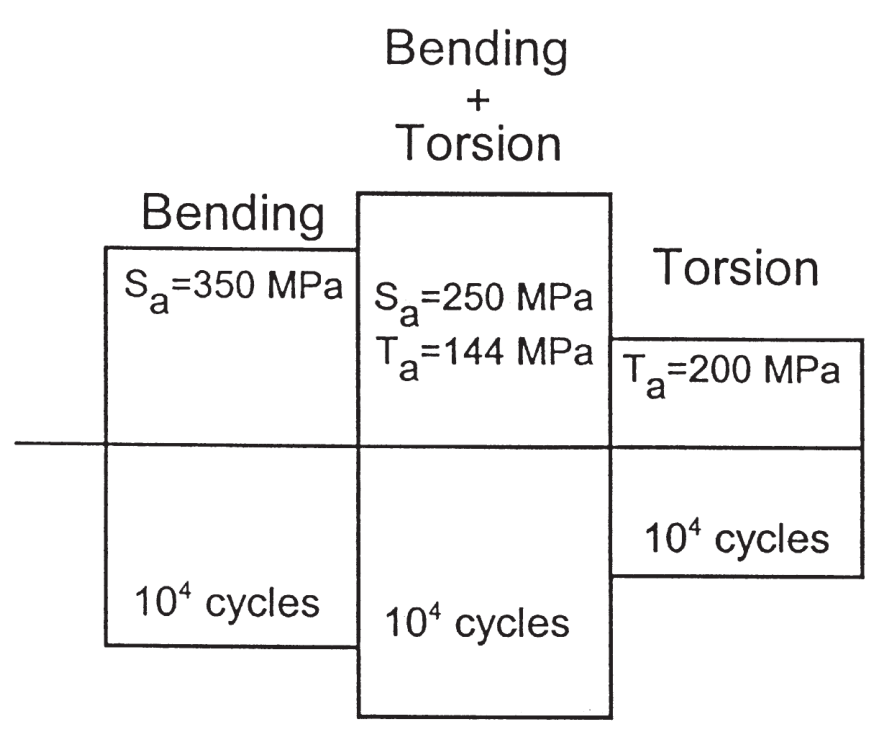
\includegraphics[width=0.6\textwidth]{figures//block.png} 
	\caption{block sequence tests (bending/bending+torsion/torsion) performed on a mild
		steel XC18.}
	\label{block}
\end{figure} 

Let us consider now a block sequence composed of
$10^4$ cycles of bending ($\Sigma_a =350 MPa$) followed by $10^4$
cycles of combined in-phase bending–torsion ($\Sigma_a ,T_a =250 MPa, 144 MPa$)
followed by $10^4$ cycles of torsion ($T_a =200 MPa$). This
sequence is repeated until the initiation of a crack. The
mean lifetime is found to be $N=1.73\times10^5$ .

The three generalized fatigue
limits relative to the three blocks are estimated according
to Eq.\eqref{taus}:

$$\tau_{lim}^{bending}=155 MPa$$   $$\tau_{lim}^{torsion}=179 MPa$$  $$\tau_{lim}^{bend+tors}=157 MPa$$


These three values and the parameter $q$ are enough to
accumulate the damage in the three blocks using Eq.\eqref{NFsimple}:


$$\frac{\Gamma^{(bending)}}{\Gamma_R^{(bending)}}+\frac{\Gamma^{(bend+tors)}}{\Gamma_R^{(bend+tors)}}+\frac{\Gamma^{(torsion)}}{\Gamma_R^{(torsion)}}=1$$

The corresponding number of cycles to initiation is:
$N_{prediction} <1.5\times10^5$ , that is to say five successive applications of the sequence. This prediction, close to the experimental result $N=1.73\times10^5$ , is a conservative one.

It is important to note that if only one critical plane
(either from bending, torsion or bending+torsion
loading) is used for damage accumulation, one-third of
the damage would be calculated, resulting in a nonconservative prediction.

Morel's method is promising in its description aspect of limited endurance fatigue phenomenon, through the choice of the  mesoscopic plastic deformation. By using cumulative plasticity, a fatigue mechanisms occurring at the mesoscopic scale takes into account the main factors affecting the lifetime cycle fatigue (hydrostatic pressure and influence of phase shift). 

However, at the present stage, it does not completely meet the demand of a predictive tool. Indeed, it is a relatively complicated method (search critical plane $\Delta_c$ and accumulated damage in each direction in the plan); its application for multiaxial variable amplitude fatigue loads requires data that are still not available (an S-N curve, two endurance limits and a particular  damage accumulation test). Moreover, it is not completely free of counting method because its author uses the counting of the extrema of the evolution of the resolved shear $T_a$ to get the macroscopic resolved shear stress $T_A$ and the corresponding amplitude $P_a$ and mean values $P_m$ of the hydrostatic stress in each direction (m) in $\Delta_c$. Again, this makes it difficult and daunting task.
 % Experiment 2
%%!TEX root=../Thesis_Zepeng.tex
\chapter{Space gradient effects}\label{chp:3}
\minitoc

\vspace{6pt}
\textbf{This chapter is based on the paper entitled``Multi-axial Fatigue Criteria with Length Scale and Gradient Effects'' }(\cite{zepeng2015multi})
\vspace{6pt}

The objective of the work is first to extend some classic high cycle fatigue (HCF) criteria (as Crossland, Dang Van, Papadopoulos, ...) introduced in Chapter \ref{chp:2} in order  to take into account a sensitivity of the criteria to stress spatial variations occurring at length scale $l_g$, and second to compare the performances of the extensions through several experimental fatigue tests. After an introduction of the basic criteria and their gradient based extensions proposed by Luu et al., we focus on the Crossland criterion and we  propose a more practical and simple expression taking into account the gradient of the stress amplitude and the maximum hydrostatic stress. The generalization of the approach to other multiaxial fatigue criteria is also proposed.  The proposition is then tested and applied to different simple situations such as 4-point bending and cantilever rotative bending.  The relative errors between the exact solutions and the experimental data are estimated. Biaxial  bending-torsion tests are also simulated to demonstrate the capabilities of the approach.  In this work only stress gradient with a beneficial effect on fatigue have been considered. 

\section{Introduction}

In several industries, the required design lifetime of many components often exceeds $ 10^8 $ cycles. This requirement is applicable to aircraft (gas turbine disks $ 10^{10} $ cycles), automobiles (car engine $ 10^8 $ cycles), and railways (high speed train $ 10^9 $ cycles) (\cite{wachtman2009mechanical}). Although a large amount of fatigue data has been published in the form of S-N (where S is stress and N  the number of cycles to fatigue) curves, the data in the literature have been usually limited to fatigue lives up to $ 10^7 $ cycles. Beyond that, a near hyperbolic relationship between stress and fatigue life is assumed, with an asymptotic limit defined as the fatigue limit (or endurance stress). 
A large number of multiaxial fatigue criteria, generalizing this notion of fatigue limit, are available in the literature (\cite{Papadopoulos1997219}, \cite{ballard1995high}, \cite{suresh1998fatigue}). They are  used to design industrial components against failure. Nevertheless, most of these criteria present some drawbacks,  for instance when dealing with out-of-phase loading or with metals of different kinds from those used to develop the criteria. In fact, most of them are not designed to cope with high stress gradients such as those introduced  by surface treatments or notches, or to handle  scale effects as  specially present in nano or micro components. 

More precisely, as mentioned by Luu et al. (\cite{luu2014formulation}), in problems related to small electronic components and electro-mechanical devices, at sufficiently small sizes, factors as size, gradient and loading effects affecting fatigue limits are not captured by classical fatigue criteria. In particular,  for the same stress distribution as well as nominal maximum stress of the material, the smaller the sample size is, the smaller the surface or the volume of the most stressed zone is, the higher the fatigue limit is.  Moreover, the nominal fatigue limit increases in the presence of stress gradient corresponding to a decreasing stress from the surface. Papadopoulos illustrates with experimental example and makes clearer the ``beneficial gradient effect" (\cite{Papadopoulos1996513}). 

The quantitative estimate of the contribution of the pure size effect made in \cite{Papadopoulos1996513}, using the results of the constant moment tests on specimens of the same radius but different lengths(\figref{fig.sizeeffect}(a)) or of the same length with different radius(\figref{fig.sizeeffect}(b)), is recalled and
used. The slope of the linear trend observed for the (fatigue limit-R)
data in \figref{fig.sizeeffect}(b) is much higher than the one for the (fatigue limit-L) data in \figref{fig.sizeeffect}(a).
\begin{Figure}[!h]{Constant moment bending fatigue limit data: (a) constant radius R; (b) constant length L (Results of Pogoretskii and Karpenko\cite{Pogoretskii1966}, represented by Weber\cite{weber1999fatigue}).}[fig.sizeeffect]
	\graphfile*[34]{figures//sizeeffect_length.png}[]
	\graphfile*[34]{figures//sizeeffect_radius.png}[]
\end{Figure}

The results of the constant moment tests on specimens of the same radius but different lengths shows that the gradient effect is an order of magnitude higher than the pure size effect. In this case, size effect is proved insignificant compared to the gradient effect at the considered scale. Once the gradient correction is made and a proper multiaxial criterion is used, it appears that the size effect due to increasing the loaded surface area at the notch tip for the different geometries is negligible compared to the gradient effect.

From above it is concluded that the stress gradient factor is the most important contributer to the beneficial effect phenomenon. Fatigue criteria have been generalized by several authors by including a  gradient dependence (\cite{Papadopoulos1996513}) in order to introduce a sensitivity of the endurance limit to difference in stress as a function of length along a gradient field occurring at length scale  $l_g$. Uniaxial normal cyclic stress states with non-zero and zero normal stress gradients, respectively,give some indication about the normal stress gradient effect. The larger the normal stress due to bending, the larger the difference between bending test points and tension-compression ellipse arc (as is shown in \figref{fig2}).
\begin{figure}[!h]
	\centering
	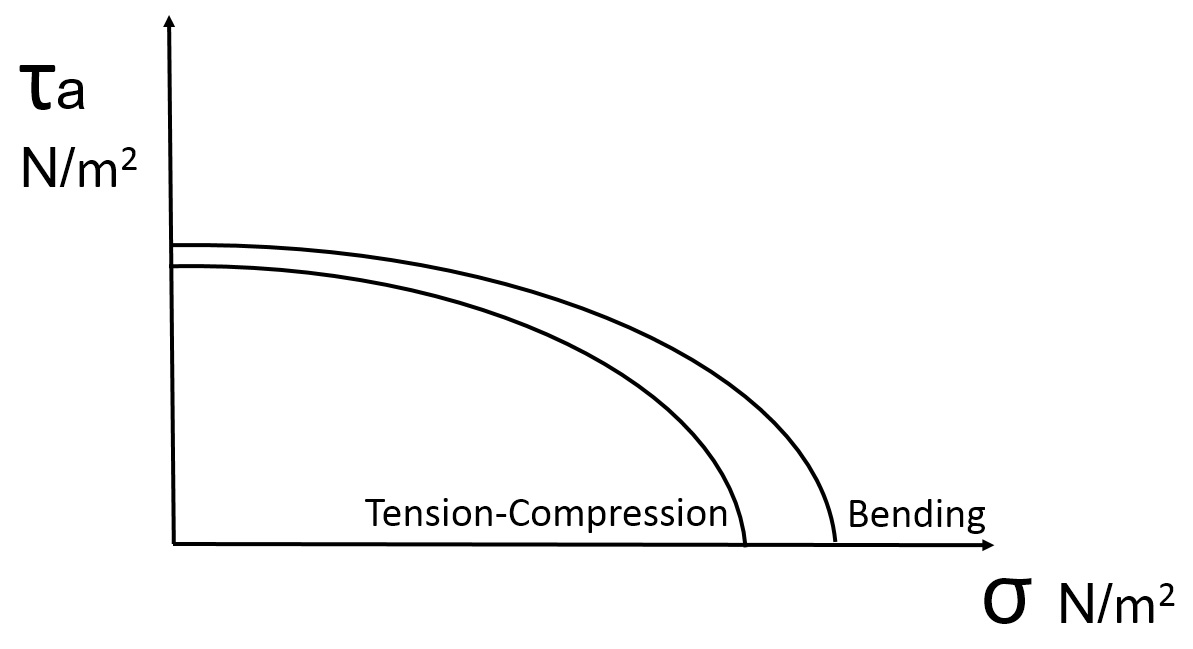
\includegraphics[width=0.8\textwidth]{figures//fig2.jpg} 
	\caption{Schematic representation of the nominal fatigue limit (ellipse arc) for two different tests: the arc is larger in the case of bending-torsion (presence of stress gradient) than in tension-compression.}
	\label{fig2}
\end{figure}

Apart from gradient approaches (\cite{Amargier20101904}, \cite{Papadopoulos1996513}), to take into account the beneficial effect, others approaches such critical volume (\cite{maitournam2009fatigue}), critical distance (\cite{taylor2010theory}, \cite{Araujo200795}), critical layer (\cite{flavenot1983epaisseur}), averaging over a specific volume (\cite{palin2000stress}, \cite{Banvillet2003755}) are used . In fact, all the approaches are equivalent to introducing a length scale. 
In the paper, we consider specifically the gradient approach. We start from the proposition of Luu et al., and propose and analyze a simpler way to account for the gradient effect at a specific length scale. The Crossland criterion (\cite{crossland1956effect}), one of the most widely known HCF criteria, is used to illustrate the approach. Crossland proposed that the second invariant of the deviatoric stress tensor and the hydrostatic stress are the variables governing the endurance limit. 
The new proposition adds two gradient terms ; it is then calibrated and its predictions are compared to experimental results to check its relevancy.


\section{A first gradient approach (\cite{luu2014formulation})}
\subsection{General formulation}

Luu et al. \cite{luu2014formulation} proposed extensions of classical HCF fatigue criteria using the gradients of the shear and normal stress to account for the gradient effect. In the case of critical plane type criteria, they defined a generalized shear stress amplitude including shear stress gradient and a generalized maximum normal (or hydrostatic) stress.
A general form of classical fatigue limit criteria can be written as follows:
\begin{equation}
	\label{eq:classical}
	f(C_a(n^*),N_{max}(n^*))=C_a(n^*)+aN_{max}(n^*)-b\geqslant 0 ,
\end{equation}
with a, b being two material parameters. $f$ is a function, chosen in many cases as linear, and $n^*$ is the normal vector of the critical plane; $C_a(n^* )$, $N_{max} (n^* )$ are respectively the amplitude of shear stress and the maximum value of the normal stress on the critical plane.

A new class of fatigue criteria extended from classical ones with stress gradient terms introducing not only in the normal stress but also in the shear stress components, was proposed in \cite{luu2014formulation}. It concerns only defect free materials and can model both phenomena ``smaller is Stronger and Higher Gradient is Stronger". 

Besides the stress gradient term appearing in the normal stress part in form of $G=\Delta(\sigma_{11}+\sigma_{22}+\sigma_{33})$, another gradient term, the gradient of the stress tensor amplitude (or alternatively of deviatoric stress tensor amplitude) $\parallel{Y}_a\parallel={\Delta\sigma}_a$ is added to the shear stress amplitude part. Basing on all these analyses a new form of fatigue criteria taking into account gradient effects, is proposed:
\begin{equation}
	f(\widetilde{C_a}(n^*),\widetilde{N_{max}}(n^*))=\widetilde{C_a}(n^*)+a\widetilde{N}_{max}(n^*)-b\geqslant 0 ,
	\label{eq:gradient crossland}
\end{equation}
where $\widetilde{C_a}(n^*)$ and $\widetilde{N_{max}}(n^*)$ are extended definitions of the amplitude of shear stress and of the normal stress taking into account the presence of local gradient.

In the following we first focus on the Crossland criterion and its extension.

\subsection{The classical Crossland criterion}

The classical Crossland criterion (\cite{crossland1956effect}) defines the fatigue limit of metallic specimens subjected to multi-axial cyclic stress  by : 
\begin{equation}
	f(\sqrt{J_{2,a}},\sigma_{H,max})=\sqrt{J_{2,a}}+a\sigma_{H,max}-b\leqslant 0,\label{eq:crossland}
\end{equation}
where $\sqrt{J_{2,a}}$ measures  the amplitude of variation of the second invariant of the deviatoric stress  and $\sigma_{H,max}$ is the maximum hydrostatic stress observed during a loading cycle. The parameters $a$ and $b$ are material constants to be calibrated experimentally. The amplitude of the square root of the second invariant of the stress deviator can be defined, in general case, as the half-length of the longest chord of the deviatoric stress path or as the radius of the smallest hypersphere circumscribing the stress deviator loading path (\cite{Papadopoulos1997219})
\begin{equation}\sqrt{J_{2,a}}=\sqrt{\frac{1}{2}\min \limits_{\uline{\uline{S_1}}}\left\lbrace \max \limits_{t}\left( (\uline{\uline{S}}(t)-\uline{\uline{S_1}}):(\uline{\uline{S}}(t)-\uline{\uline{S_1}})\right) \right\rbrace }.\end{equation}

The deviatoric stress $\uuline{S}$ associated with a stress tensor $\uuline{\sigma}$  is defined by
\begin{equation} \uuline{S}=\uuline{\sigma}-\dfrac{1}{3}\textrm{tr}\uuline{\sigma}\, \uuline{I},
\end{equation}
where $\textrm{tr}\uuline{\sigma}$ is the trace of the stress tensor $\uuline{\sigma}$ and $\uuline{I}$ the second order unit tensor.

The maximum value that the hydrostatic stress reaches during the loading cycle is on the other hand:
\begin{equation}
	\sigma_{H,max}=\max\limits_{t}\left\lbrace \dfrac{1}{3}\textrm{tr}(\uuline{\sigma}(t))\right\rbrace .
\end{equation}

For a proportional cyclic loading, if one introduces the two extreme stress tensors $\uuline{\sigma}^A$ and $\uuline{\sigma}^B$ observed during the loading path, together with the stress range 
\begin{equation}\uuline{\Delta\sigma}=\uuline{\sigma}^B-\uuline{\sigma}^A\end{equation}
and its deviatoric part $\uuline{\Delta s} $, the variation of
the second invariant of the stress deviator reduces to 
\begin{equation}\sqrt{J_{2,a}}=\dfrac{1}{2}\max\limits_{t}\sqrt{\dfrac{1}{2}\uuline{\Delta s}:\uuline{\Delta s}}=\dfrac{1}{2}\max\limits_{t}\sqrt{\dfrac{1}{2}\left( \Delta s_{11}^2+\Delta s_{22}^2+\Delta s_{33}^2+2\Delta s_{12}^2+2\Delta s_{13}^2+2\Delta s_{23}^2\right) }.\end{equation}



The material constants $a$ and $b$ can be related to  the limit $t_{-1}$ of endurance in alternate torsion and to the limit $s_{-1}$ of endurance in alternate tension-compression by
\begin{equation}
	a=\dfrac{3 t_{-1}}{s_{-1}}-\sqrt{3},\quad 
	b=t_{-1}.
	\label{crossland-ab}
\end{equation}

\subsection{Formulation of Crossland criterion with gradient effect}

In particular, using as a basis the classical Crossland criterion Eq.\eqref{eq:crossland} and the general framework for the development of a gradient dependent fatigue limit criterion Eq.\eqref{eq:gradient crossland}, a new version can be written in the form:
\begin{equation}
	\sqrt{\widetilde{J_{2,a}}}+a\widetilde{\sigma_{H,max}}\leqslant b .
\end{equation}

This formula takes into account the indicator of the influence of the gradient of the stress deviator which reflects the spatial non-uniform distribution of stress state.

In practice, \cite{luu2014formulation} had proposed:
\begin{equation}
	\sqrt{{J_{2,a}}}\sqrt{1-\left(l_\tau\dfrac{\parallel \uuline{\uline{Y}}\parallel_{,a}}{\parallel \uuline{S}\parallel_{,a}}\right)^{n_\tau}}+a\sigma_{H,max}\left(1-\left\langle  l_\sigma\dfrac{\parallel G\parallel}{\sigma_{H,max}}\right\rangle ^{n_\sigma}\right)-b < 0 .
\end{equation}

Here $\parallel \uuline{\uline{Y}}\parallel_{,a}$ is the full stress gradient and $\parallel G\parallel$ is used as an indicator of the influence of the normal stresses gradient.

\begin{equation}
	\parallel{G}\parallel=\parallel{\nabla \sigma_{H,max}}\parallel=\sqrt{\left(\dfrac{\partial \sigma_{H,max}}{\partial x}\right)^2+\left(\dfrac{\partial \sigma_{H,max}}{\partial y}\right)^2+\left(\dfrac{\partial \sigma_{H,max}}{\partial z}\right)^2} .
\end{equation}



\section{Optimized Crossland Criterion formulation}
The precedent Luu and al. formula has six materials parameters $a$,$b$,$l_\tau$,$l_\sigma$,$n_\tau$,$n_\sigma$ to be identified experimentally. The calibration can be complicated ; it does not lead to a unique set of parameters. Physical considerations, such as the length scales, have to be taken into account for choosing the optimized material constants. For practical application in an industrial context, it is essential to reduce the number of parameters. We therefore wish to investigate a simpler construction, departing from the classical Crossland criterion.

Surfaces with stresses decreasing in depth are, here and after, considered. Failure occurs at the point $x_0$ when,  $(\sqrt{J_{2,a}}+a\sigma_{H,max}-b)(x_0)\geqslant 0 $. To be more general and avoid singularity, this condition should be satisfied in some $x_0$ neighboring volume of size $l_g$, leading to a criterion given by:

\begin{equation}
	\inf\limits_{\uline{x}\in B\left( \uline{x_0},\,\uline{l_g}\right) }\left( \sqrt{J_{2,a}}+a\sigma_{H,max}-b\right) (x)\geqslant 0 .
	\label{crossland-x0-2}
\end{equation}

To obtain a suitable expression, an expansion of Eq.(\ref{crossland-x0-2}) in performed in the neighborhood of ${x_0}$. The sought formula should account for the beneficial effect of the stress gradient. Considering that the stress is decreasing in depth, we consider the most favorable point in the neighborhood(inf) thus  a negative sign is associated with the norm of the gradient of stress tensor in to the proposed formula. In addition, the gradient term should not only affect hydrostatic stress but also shear stress.

An objective formulation based on the maximum value of deviatoric stress invariants $\sqrt{J_{2,a}}$ and of $\sigma_{H,max}$ in the neighborhood, is finally:

\begin{equation}
	\sqrt{J_{2,a}}+a\sigma_{H,max}-l_g\parallel{\nabla\sqrt{J_{2,a}}}+a\nabla{\sigma_{H,max}}\parallel\leqslant b ,
	\label{modified Crossland}
\end{equation}
In this updated model, we keep the same material parameters $a$ and $b$ as before, and $l_g$ is a characteristic length to be optimized to match the experimental results. The approach has thus only one supplementary material constant, $l_g$, whose calibration is easy.

\section{Optimized Papadopoulos Criterion formulation}
As seen in Chapter\ref{chp:2}, Papadopoulos (\cite{papadopoulos1993fatigue}) has proposed to opt for a mean value of the accumulated plastic strain on all possible slip systems of representative elementary volume(REV). So he chose to use an average value  of accumulated plastic deformation rather than looking at failure of a single crystal. A spherical coordinate system(\figref{figpapa}) to guide the vector of normal in material plane, and the unit orientation vector $r$ linked to a sliding direction of this plane is used to conduct the integration over all possible orientations.

\begin{figure}[h!]
	\centering
	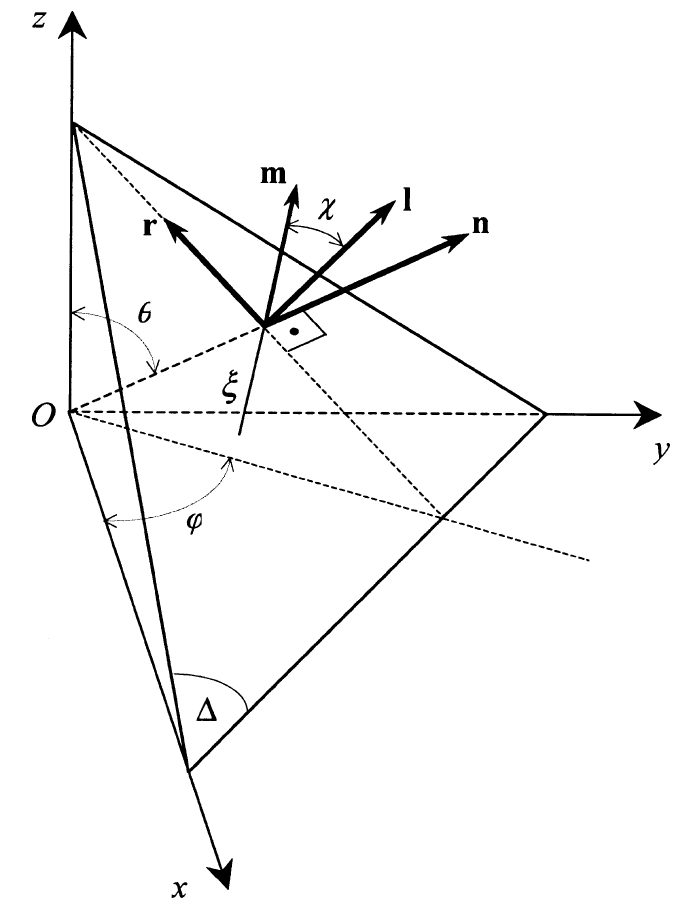
\includegraphics[width=0.5\textwidth]{figures//demopp.png} 
	\caption{Material plane $\Delta$ passing through point O of a body and its
		associated (n, l, r) frame.}
	\label{figpapa}
\end{figure}
At any point $O$ of a body, a material plane $\Delta$ can be defined by its unit normal vector $\bf n$. This vector
$\bf n$ makes an angle $\theta$ with the z-axis of a $Oxyz$ frame attached to the body, and its projection on the $xy$ plane
makes an angle $\varphi$ with axis $x$. For each plane $\Delta$ a new quantity is introduced as the quadratic mean value, over all the sliding directions of the considered plane, of the resolved shear stress amplitude and denoted as $T_a$.This shear stress quantity was first introduced in Papadopoulos\cite{Papadopoulos1996513}
and was subsequently used by other researchers.The critical plane according to his proposal is that onto which $T_a(\varphi,\theta)$ achieves its maximum value. The fatigue limit criterion is written as:
\begin{equation}
	max T_a+\alpha_\infty \sigma_{h,max}\leqslant \gamma_\infty
	\label{eq.papa}
\end{equation}
where $\alpha_\infty$ and $\gamma_\infty$ are material parameters to be determined\cite{papadopoulos2001long}.
$$\sigma_{h,max}=\max\limits_{t}\left\lbrace \dfrac{1}{3}tr(\uline{\uline{\sigma}}(t))\right\rbrace. $$
As seen earlier, the construction of $T_a$ is based on the calculation of a local shear stress $\tau$:
\begin{equation}
	\begin{split}
		\tau=&[sin\theta cos\varphi\sigma_{xx}+sin\theta sin\varphi\sigma_{xy}+cos\theta\sigma_{xz}](-sin\varphi cos\chi-cos\theta cos\varphi sin\chi)+\\&[sin\theta cos\varphi\sigma_{xy}+sin\theta sin\varphi\sigma_{yy}+cos\theta\sigma_{yz}](cos\varphi cos\chi-cos\theta sin\varphi sin\chi)+\\&[sin\theta cos\varphi\sigma_{xz}+sin\theta sin\varphi\sigma_{yz}+cos\theta\sigma_{zz}]sin\theta sin\chi
	\end{split} 
	\label{eqres}
\end{equation}
It is clear that this shear stress is a function of
$\varphi$, $\theta$, $\chi$ and of time $t$ in the case of variable amplitude and out-of-phase loading, i.e. $\tau=\tau(\varphi, \theta, \chi, t)$. Upon fixing a pair of angles $(\varphi, \theta)$ (i.e. a plane
$\Delta$) and an angle $\chi$ (i.e. a line $\xi$ on $\Delta$), one can define the amplitude of the resolved shear stress $\tau_a$, acting on $\Delta$
along $\xi$ by the formula:
\begin{equation}
	\tau_a(\varphi,\theta,\chi)=\dfrac{1}{2}\big[\max \limits_{t\in P}\tau_a(\varphi,\theta,\chi ,t)-\min \limits_{t\in P}\tau_a(\varphi,\theta,\chi ,t)\big]
\end{equation}
Now, for a given plane $\Delta$, i.e. for a fixed pair of angles ($\varphi$, $\theta$),
the generalized shear stress amplitude $T_a$ is defined as the $L^2$ average in the plane $\Delta$ of the amplitude of resolved shear stress:
\begin{equation}
	T_a(\varphi,\theta)=2\sqrt{\dfrac{1}{\pi}\int_{x=0}^{\frac{\pi}{2}} \tau_a^2(\varphi,\theta,\chi)d\chi}
	\label{Ta}
\end{equation}
We note the fatigue limit in fully reversed torsion $t_{-1}$ and the fatigue limit in fully reversed bending $f_{-1}$. From these two tests we get the parameters from Eq.\ref{eq.papa}:
$$\gamma_\infty=t_{-1},$$ 
$$\alpha_\infty=3\left( \dfrac{t_{-1}}{f_{-1}}-\dfrac{1}{2}\right) .$$
The Papadopoulos fatigue limit criterion is therefore:
\begin{equation}
	maxT_a+3\left( t_{-1}/f_{-1}-1/2\right) \sigma_{h,max}\leqslant t_{-1}.
	\label{eq:papadopoulos}
\end{equation}
Now,  the Papadopoulos Criterion can be simply extended  to cases with gradient effects by
\begin{equation}
	maxT_a+\alpha_\infty\sigma_{H,max}-l_g\parallel\nabla{maxT_a}+\alpha_\infty\nabla\sigma_{H,max}\parallel\leqslant \gamma_\infty .
	\label{eq:modified papa}
\end{equation}

\section{Optimized Dang Van Criterion formulation}
The Dang Van criterion as presented in \cite{ballard1995high} and reviewed in Chapter \ref{chp:2} is expressed as:
\begin{equation}
	\max \limits_{\vec{n}}\left\lbrace \max \limits_{t}\left\{\tau{(\vec{n},t)}+a_D\sigma_H(t)\right\}\right\rbrace \leqslant b_D.
	\label{dv}
\end{equation}

Here, $\tau$ denotes the mesoscopic shear stress and is obtained from a mesoscopic stress tensor $\hat{\bm{\sigma}}$ defined by:
$$\hat{\bm{\sigma}}(t)=(\bm{\sigma}(t)-s^\star),$$
where $s^\star$ is the center of the smallest hypersphere circumscribed to the loading path in deviatoric stress space. It is obtained by solving a ``min-max" problem as follows:
$$s^\star = arg \min\limits_{s_1}\left\{\max\limits_t\parallel s(t)-s_1\parallel\right\}.$$
In the case of fully reversed loading, the values $s^\star=0$ can be directly deduced without solving the ``min-max problem" as in general case.

The principal stress values of stress tensor $\widetilde{\sigma}$ being denoted  by $\hat{\sigma}_{\Rmnum{3}}(t)\leqslant\hat{\sigma}_{\Rmnum{2}}(t)\leqslant\hat{\sigma}_{\Rmnum{1}}(t)$, one gets the maximum shear stress by:
$$\tau(t)=\dfrac{1}{2}\left( \hat{\sigma}_{\Rmnum{1}}(t)-\hat{\sigma}_{\Rmnum{3}}(t)\right) .$$
Moreover, $\sigma_H(t)$ denotes  the hydrostatic stress as a function of the time.
The material characteristic parameters $a_D$ and $b_D$ are finally  given from traction compression and torsion fatigue limits by  :
$$a_D=\dfrac{3t_{-1}}{s_{-1}}-\dfrac{3}{2};$$  $$b_D=t_{-1}.$$

Now,  the Dang Van criterion can be extended to a gradient dependent criterion by 
\begin{equation}
	\max \limits_{t}\left\{\tau{(t)}+a_D\sigma_H(t)\right\}-l_g\parallel	\max \limits_{t}\left\{{\nabla\tau{(t)}}+a_D\nabla\sigma_H(t)\right\}\parallel\leqslant b_D.
	\label{modified dangvan}
\end{equation}
\section{Calibration of the critera}

In this section, two different uniaxial fatigue tests with stress gradient effects are used to calibrate the optimized gradient Crossland, Papadopoulos and DangVan criteria. An application to a biaxial test fatigue test shows the ability of the proposed approach to account for stress gradient in multiaxial cases. 


\subsection{Fully reversed 4-point bending and rotating cantilever bending fatigue tests}
\subsubsection{With Crossland criterion}
The model of 4-point bending is first considered. The bar made of steel has both ends fixed. The radius $R$ is a variable ranging from 1mm to 30mm in order to  challenge the fact ``the smaller, the stronger". The length $L$ of the bar is 100 mm.

\begin{figure}[h!]
	\centering
	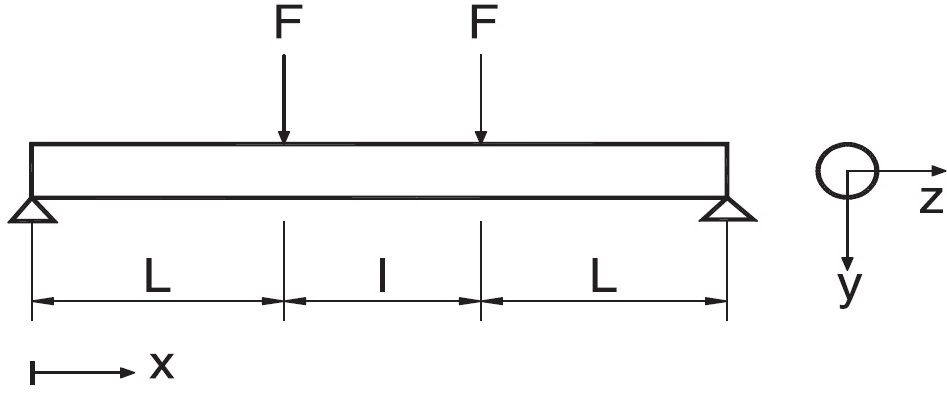
\includegraphics[width=0.4\textwidth]{figures//fig11.jpg} 
	\caption{4-point bending test (\cite{Papadopoulos1996513}) }
	\label{fig11}
\end{figure}

The bending moment is the same in the interval $L\leqslant x \leqslant L+l$ and equal to
$M = FL$ (\figref{fig11}).
For $L\leqslant x \leqslant L+l$ and  $-R\leqslant y \leqslant R$, the bending stress $\bm{\sigma}$  is
\begin{equation}
	\uuline{\sigma}(t)=\sigma_{xx}sin(\omega t)e_x\otimes e_x=\dfrac{FLy}{I}sin(\omega t) e_x\otimes e_x \label{bending4} \end{equation}
with $I=\pi R^4/4$, $\omega$ is the angular velocity.  The maximum stress during the cyclic loading in the bar  is thus 
$ \sigma_{max}=\dfrac{FLy}{I}$, 
while the macroscopic stress range is $ \Delta\uuline{\sigma}(t)=2\sigma_{max}e_x\otimes e_x $, and the 
hydrostatics stress takes the value
\begin{equation}
	\sigma_{H,max}=\max\limits_{t}\left\lbrace \dfrac{1}{3}\textrm{tr}(\sigma(t))\right\rbrace =\dfrac{1}{3}\sigma_{max}=\dfrac{FLy}{3I}.
\end{equation}
From the value of  the deviatoric stress
\begin{equation} 
	\Delta\uuline{ S}=\Delta\uuline{\sigma}-\dfrac{1}{3}\textrm{tr}\Delta\uuline{\sigma}\uuline{I}=
	\left(
	\begin{array}{ccc}
		\dfrac{4}{3}\sigma_{max} & 0 & 0\\
		0 & -\dfrac{2}{3}\sigma_{max} & 0\\ 
		0 & 0 & -\dfrac{2}{3}\sigma_{max}\\
	\end{array}\right) ,
\end{equation}
we can compute the second invariant of the stress deviator :
\begin{equation}
	\sqrt{J_{2,a}}=\dfrac{1}{2\sqrt{2}}\sqrt{\Delta \uuline{S}:\Delta \uuline{S}}=\dfrac{\sigma_{max}}{\sqrt{3}} =\dfrac{FLy}{\sqrt{3}I} .
\end{equation}


Then the gradient part is given by:
\begin{equation}
	\nabla\sqrt{J_{2,a}}=\dfrac{\partial\sqrt{J_{2,a}}}{\partial x}\uline{e}_x+\dfrac{\partial\sqrt{J_{2,a}}}{\partial y}\uline{e}_y+\dfrac{\partial\sqrt{J_{2,a}}}{\partial z}\uline{e}_z=\left( 0,\dfrac{FL}{\sqrt{3}I},0\right)  ,
\end{equation}
and
\begin{equation}
	\nabla \sigma_{H,max}=(0,\dfrac{FL}{3I},0).
\end{equation}
The parameters $a$ and $b$ of the standard Crossland criterion, are obtained from fully reversed tension-compression fatigue limit $s_{-1}$  and torsion fatigue limit $t_{-1}$ using Eq.(\ref{crossland-ab}).

From Eq.(\ref{eq:crossland}), standard Crossland criterion without gradient effect (for radius $R$) is:
\begin{equation}
	\sqrt{J_{2,a}}+a\sigma_{H,max}=\dfrac{FLR}{\sqrt{3}I} +\dfrac{aFLR}{3I}\leqslant b.
	\label{eq4pcross}
\end{equation}
The gradient term here is given by:
\begin{equation}
	\parallel{\nabla\sqrt{J_{2,a}}}+a{\nabla \sigma_{H,max}}\parallel=\dfrac{FL}{\sqrt{3}I}+\dfrac{aFL}{3I}.
	\label{cross-gradient-term}
\end{equation}

By comparison we can see in 4-point bending test the difference between classical and modified Crossland criterion corresponds to the product of the characteristic length $l_g$ by the term (\ref{cross-gradient-term}) associated to the decrease of the stress in depth. This value shows how much the modification affects the Crossland criterion. 

\noindent Crossland criterion with beneficial gradient term as shown in Eq.(\ref{modified Crossland}) is given by:
\begin{equation}
	\begin{split}
		\sqrt{J_{2,a}}+a\sigma_{H,max}-l_g(\parallel{\nabla\sqrt{J_{2,a}}}+a\nabla{\sigma_{H,max}}\parallel)&=\\ \dfrac{FLR}{\sqrt{3}I} +\dfrac{aFLR}{3I}-l_g\left( \dfrac{FL}{\sqrt{3}I}+\dfrac{aFL}{3I}\right) 
		&=\\ \dfrac{1}{\sqrt{3}}\sigma_{max}+\dfrac{a}{3}\sigma_{max}-l_g\left( \dfrac{1}{\sqrt{3}R}\sigma_{max}+\dfrac{a}{3R}\sigma_{max}\right) &\leqslant b\, ,
	\end{split}
\end{equation}
which is to say:
\begin{equation}
	\sigma_{max}\leqslant\dfrac{b}{\dfrac{1}{\sqrt{3}}+\dfrac{a}{3}-l_g\left( \dfrac{1}{\sqrt{3}R}+\dfrac{a}{3R}\right) }\, .
\end{equation}

The material parameters $a$ and $b$ are obtained using their classical expressions as Eq.(\ref{crossland-ab}) from tests free of stress gradient. The corresponding fatigue limit are denoted $s_{ref}$ for the alternate tension-compression test, and $t_{ref}= b$ for the alternate torsion test. For a specimen of radius $R$
the alternate bending fatigue limit is denoted $f_c(R)$.
We can observe that:
\begin{equation}
	f_c(R)=\dfrac{b}{\dfrac{1}{\sqrt{3}}+\dfrac{a}{3}-l_g\left( \dfrac{1}{\sqrt{3}R}+\dfrac{a}{3R}\right) }\geqslant s_{ref} = \dfrac{b}{\dfrac{1}{\sqrt{3}}+\dfrac{a}{3}},
	\label{crossland-fr}
\end{equation}
and that $f_c(R)$ tends to $s_{ref}$ for large values of $R$.

\subsubsection{With Papadopoulos criterion}  
From Eq.\ref{bending4}, the resolved shear stress $\tau$ acting along a line $\xi$ of a plane $\Delta$ is given by Eq.\ref{eqres}, which in this case leads to:
\begin{equation}
	\tau(\varphi,\theta,\chi,t)=\sigma_{xx}sin(2\pi t/P)sin\theta cos\theta sin\chi.
\end{equation}
Clearly, for the worse case in $\chi$,  the resolved shear stress amplitude is equal to:
\begin{equation}
	\tau_a(\varphi,\theta,\chi)=\sigma_{xx}|sin\theta cos\theta sin\chi|.
\end{equation}
The generalized shear stress amplitude $T_a$ becomes:
\begin{equation}
	T_a(\varphi,\theta)=2\sqrt{\dfrac{1}{\pi}\int_{\chi=0}^{\frac{\pi}{2}}(\sigma_{xx}|sin\theta cos\theta sin\chi|)^2d\chi}
\end{equation}
The maximum value of $T_a$ is obtained at ($\theta=\pi/4$) and at ($\theta=3\pi/4$). It is equal to:
\begin{equation}
	maxT_a=\sigma_{xx}/2
\end{equation}
The hydrostatic stress is given by:
\begin{equation}
	\sigma_{H}(t)=\dfrac{1}{3}\sigma_{xx}sin(2\pi t/P)
\end{equation}
The maximum value of $\sigma_H$ reached in a loading cycle is:
\begin{equation}
	\sigma_{H,max}=\sigma_{xx}/3
\end{equation}
Papadopoulos criterion with beneficial gradient term as shown in Eq.\eqref{eq:modified papa} is then given by:
\begin{equation}
	\begin{split}
		maxT_a+\alpha_\infty\sigma_{H,max}-l_g\parallel\nabla{maxT_a}+\alpha_\infty\sigma_{H,max}\parallel&=\\\dfrac{FLR}{2I} +\dfrac{\alpha_\infty FLR}{3I}-l_g\left( \dfrac{FL}{2I}+\dfrac{\alpha_\infty FL}{3I}\right) &=\\ \dfrac{1}{2}\sigma_{max}+\dfrac{\alpha_\infty}{3}\sigma_{max}-l_g\left( \dfrac{1}{2R}\sigma_{max}+\dfrac{\alpha_\infty}{3R}\sigma_{max}\right) &\leqslant \gamma_\infty = t_{ref} ,
	\end{split}
\end{equation}
which is to say:
\begin{equation}
	\sigma_{max}\leqslant\dfrac{\gamma_\infty}{\dfrac{1}{2}+\dfrac{\alpha_\infty}{3}-l_g(\dfrac{1}{2R}+\dfrac{\alpha_\infty}{3R})} .
\end{equation}
For a specimen of radius $R$
the alternate bending fatigue limit is denoted $f_p(R)$.
We can observe that:
\begin{equation}
	f_p(R)=\dfrac{\gamma_\infty}{\dfrac{1}{2}+\dfrac{\alpha_\infty}{3}-l_g\left( \dfrac{1}{2R}+\dfrac{\alpha_\infty}{3R}\right) }\geqslant s_{ref} = \dfrac{\gamma_\infty}{\dfrac{1}{2}+\dfrac{\alpha_\infty}{3}}.
	\label{papa-fr}
\end{equation}

\subsubsection{With Dang Van criterion}  
Under fully reversed loading we have:
$$\tau(t)=\dfrac{1}{2}(\sigma_{xx}(t)-0)$$ 
From Eq.\eqref{modified dangvan} we can deduce Dang Van criterion.
\begin{equation}
	\begin{split}
		\max \limits_{t}\left\{\tau{(t)}+a_D\sigma_H(t)\right\}-l_g\parallel{\nabla\tau{(t)}}+a_D\nabla\sigma_H(t)\parallel&=\\ \dfrac{FLR}{2I} +\dfrac{aFLR}{3I}-l_g\left( \dfrac{FL}{2I}+\dfrac{aFL}{3I}\right) &=\\ \dfrac{1}{2}\sigma_{max}+\dfrac{a}{3}\sigma_{max}-l_g\left( \dfrac{1}{2R}\sigma_{max}+\dfrac{a}{3R}\sigma_{max}\right) &\leqslant b_D= t_{ref}\, ,
	\end{split}
\end{equation}
which is to say:
\begin{equation}
	\sigma_{max}\leqslant\dfrac{b}{\dfrac{1}{2}+\dfrac{a}{3}-l_g\left( \dfrac{1}{2R}+\dfrac{a}{3R}\right) }.
\end{equation}
We can observe that the corresponding bending limit is thus
\begin{equation}f_D(R)=\dfrac{b}{\dfrac{1}{2}+\dfrac{a}{3}-l_g\left( \dfrac{1}{2R}+\dfrac{a}{3R}\right) }\geqslant s_{ref} = \dfrac{b}{\dfrac{1}{2}+\dfrac{a}{3}}.
\end{equation}


\subsubsection{Comparison with experimental data}
\begin{figure}[!h]
	\begin{center}
		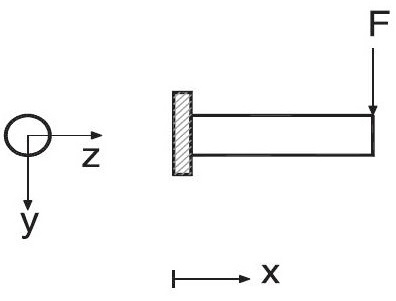
\includegraphics[width=0.5\textwidth]{figures//fig3.jpg} 
		\caption{Cantilever bending test (\cite{Papadopoulos1996513})}
		\label{fig9}
	\end{center}
\end{figure}
The case of cantilever fully reversed bending corresponds to the four point bending test except that there, the bending moment is function of $x$. Thus, the maximum stress $\sigma_{max}$ for a given section is a function of $x$. But, the $y$ dimension of the beam is much smaller than its $x$ dimension, which allows us to neglect gradients in $x$ . All  expressions of the four point bending case thus  apply to this case. 

\newpage
\begin{figure}[!h]
	\begin{center}
		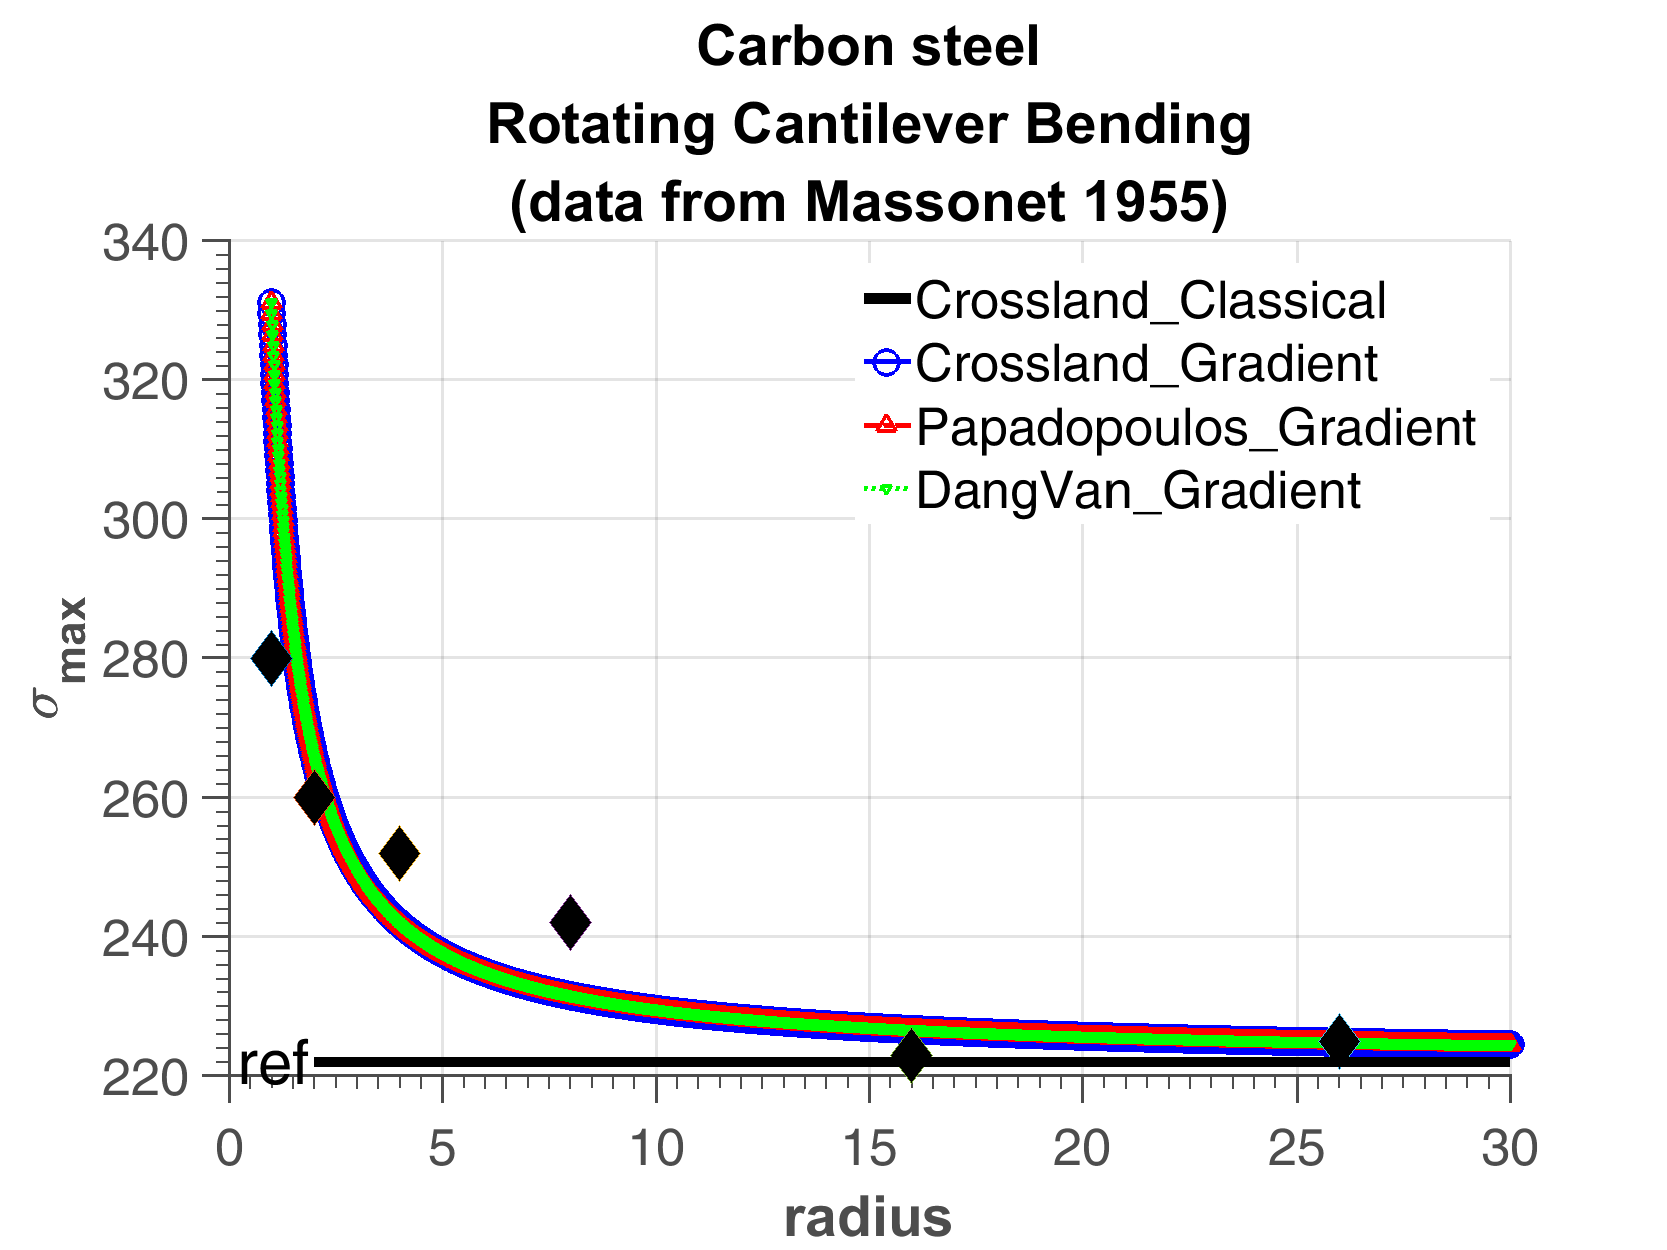
\includegraphics[width=0.9\textwidth]{figures//carbonsteel.png} 
		\caption{Fatigue limits with gradient effect for different radii (\cite{Massonnet1955}).}
		\label{fig.gradientcalibration1}
	\end{center}
\end{figure}

\begin{figure}[!h]
	\begin{center}
		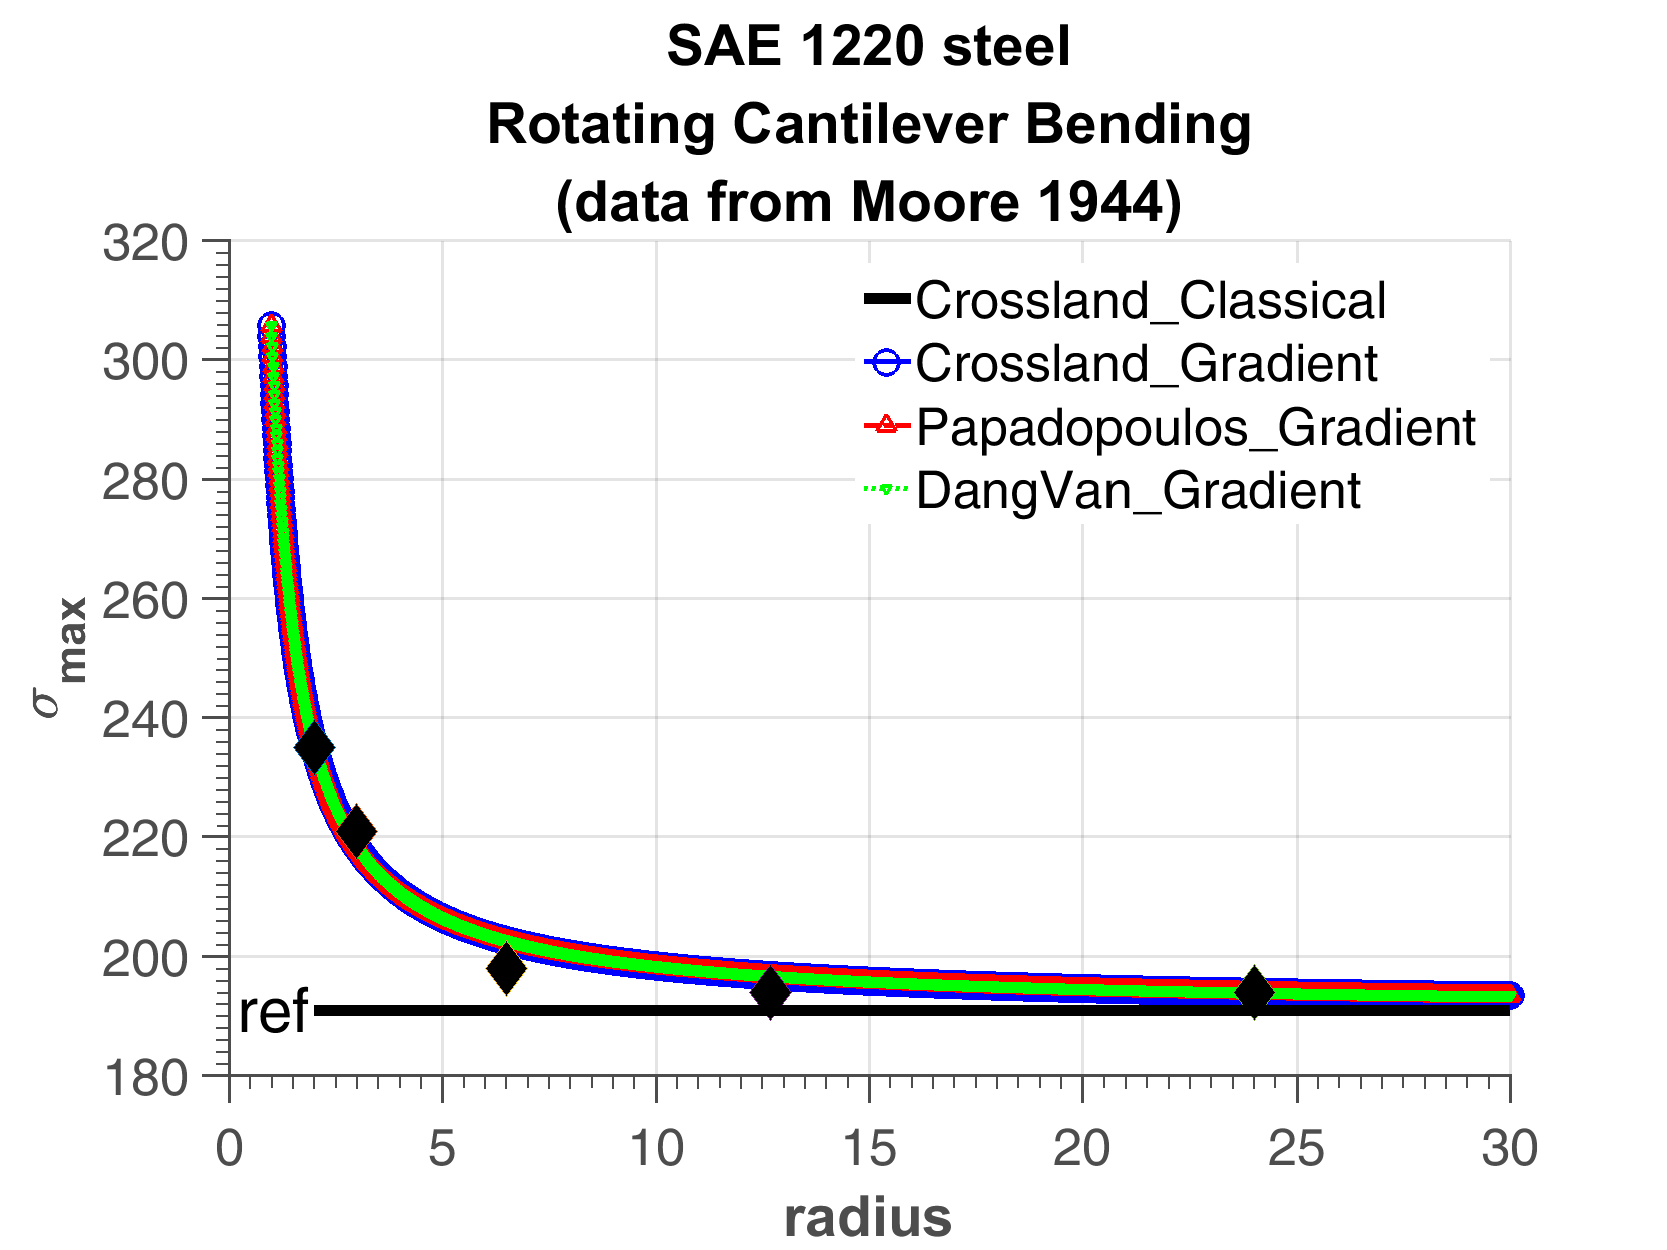
\includegraphics[width=0.9\textwidth]{figures//1220steel.png} 
		\caption{Fatigue limits with gradient effect for different radii (\cite{Moore1944}).}
		\label{fig.gradientcalibration2}
	\end{center}
\end{figure}

\begin{figure}[!h]
	\begin{center}
		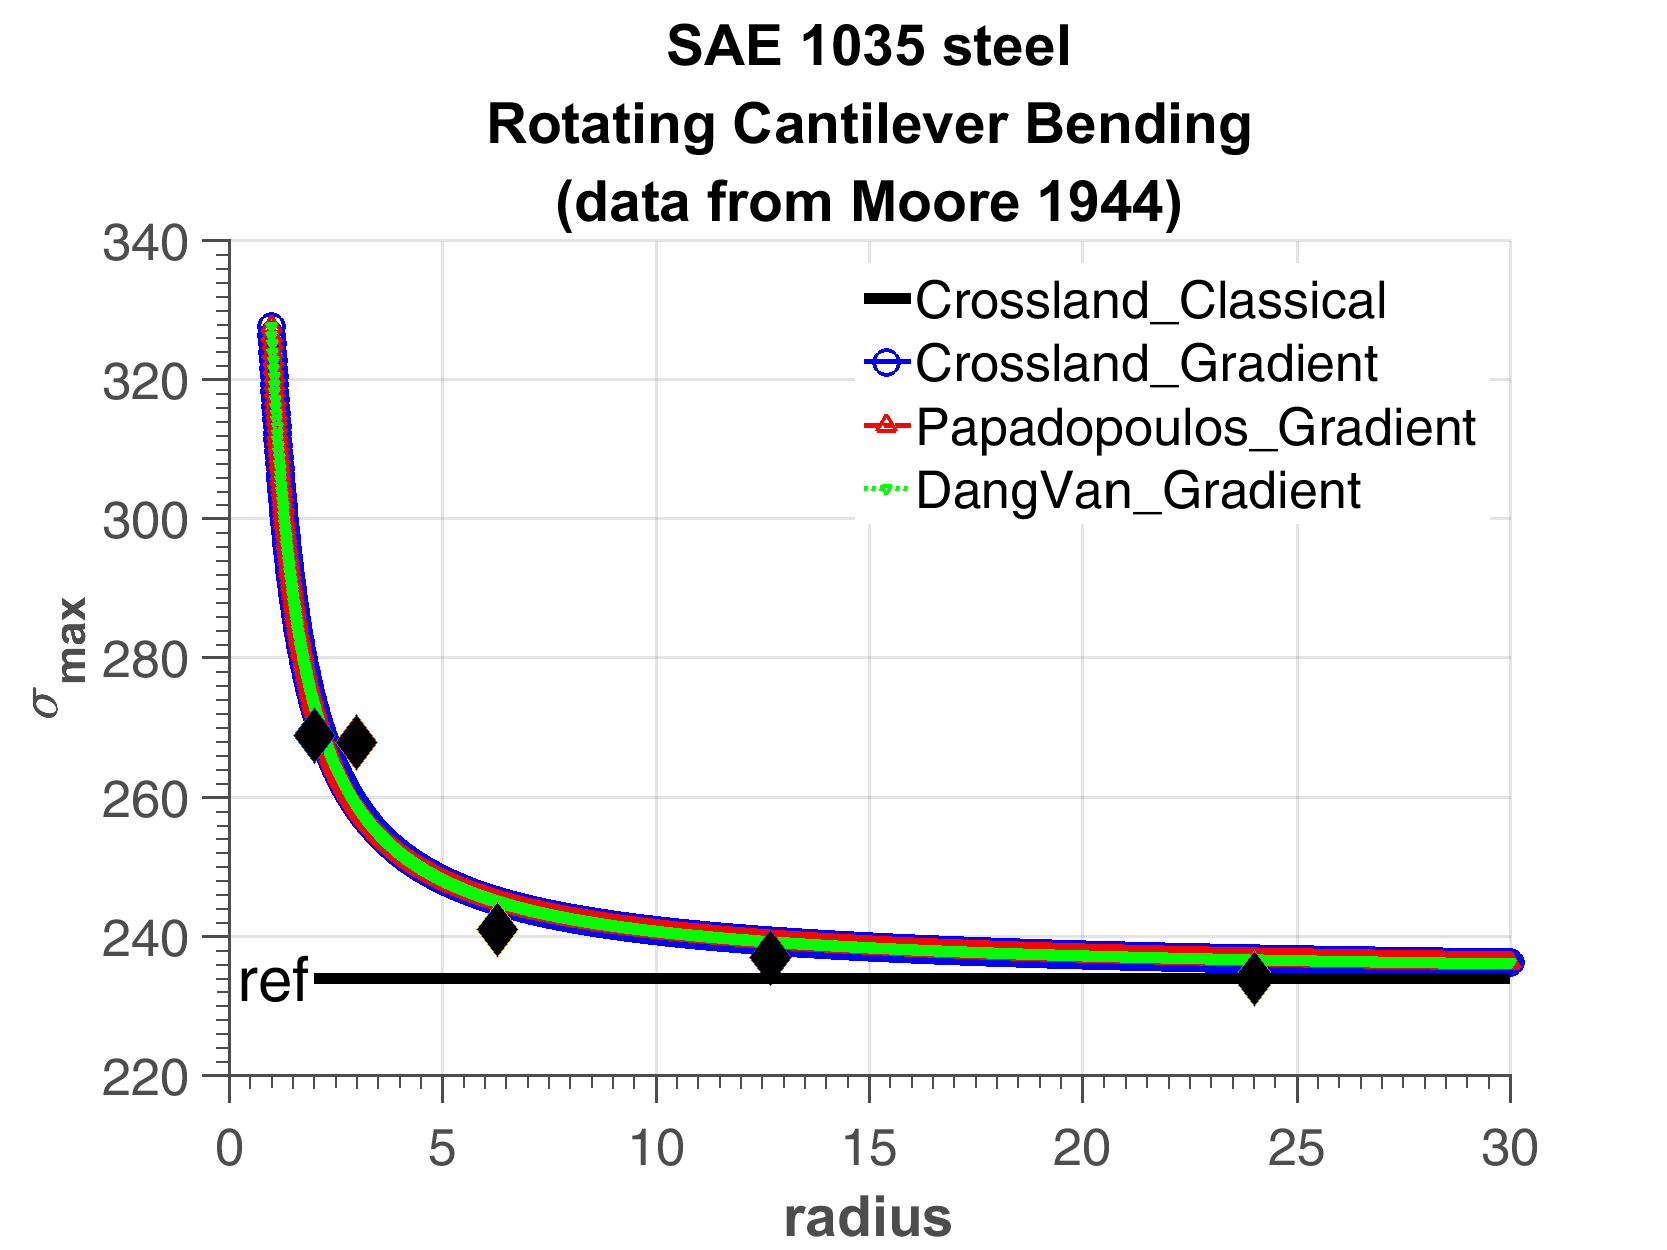
\includegraphics[width=0.9\textwidth]{figures//1035steel.png} 
		\caption{Fatigue limits with gradient effect for different radii (\cite{Pogoretskii1966}).}
		\label{fig.gradientcalibration3}
	\end{center}
\end{figure}

\begin{figure}[!h]
	\begin{center}
		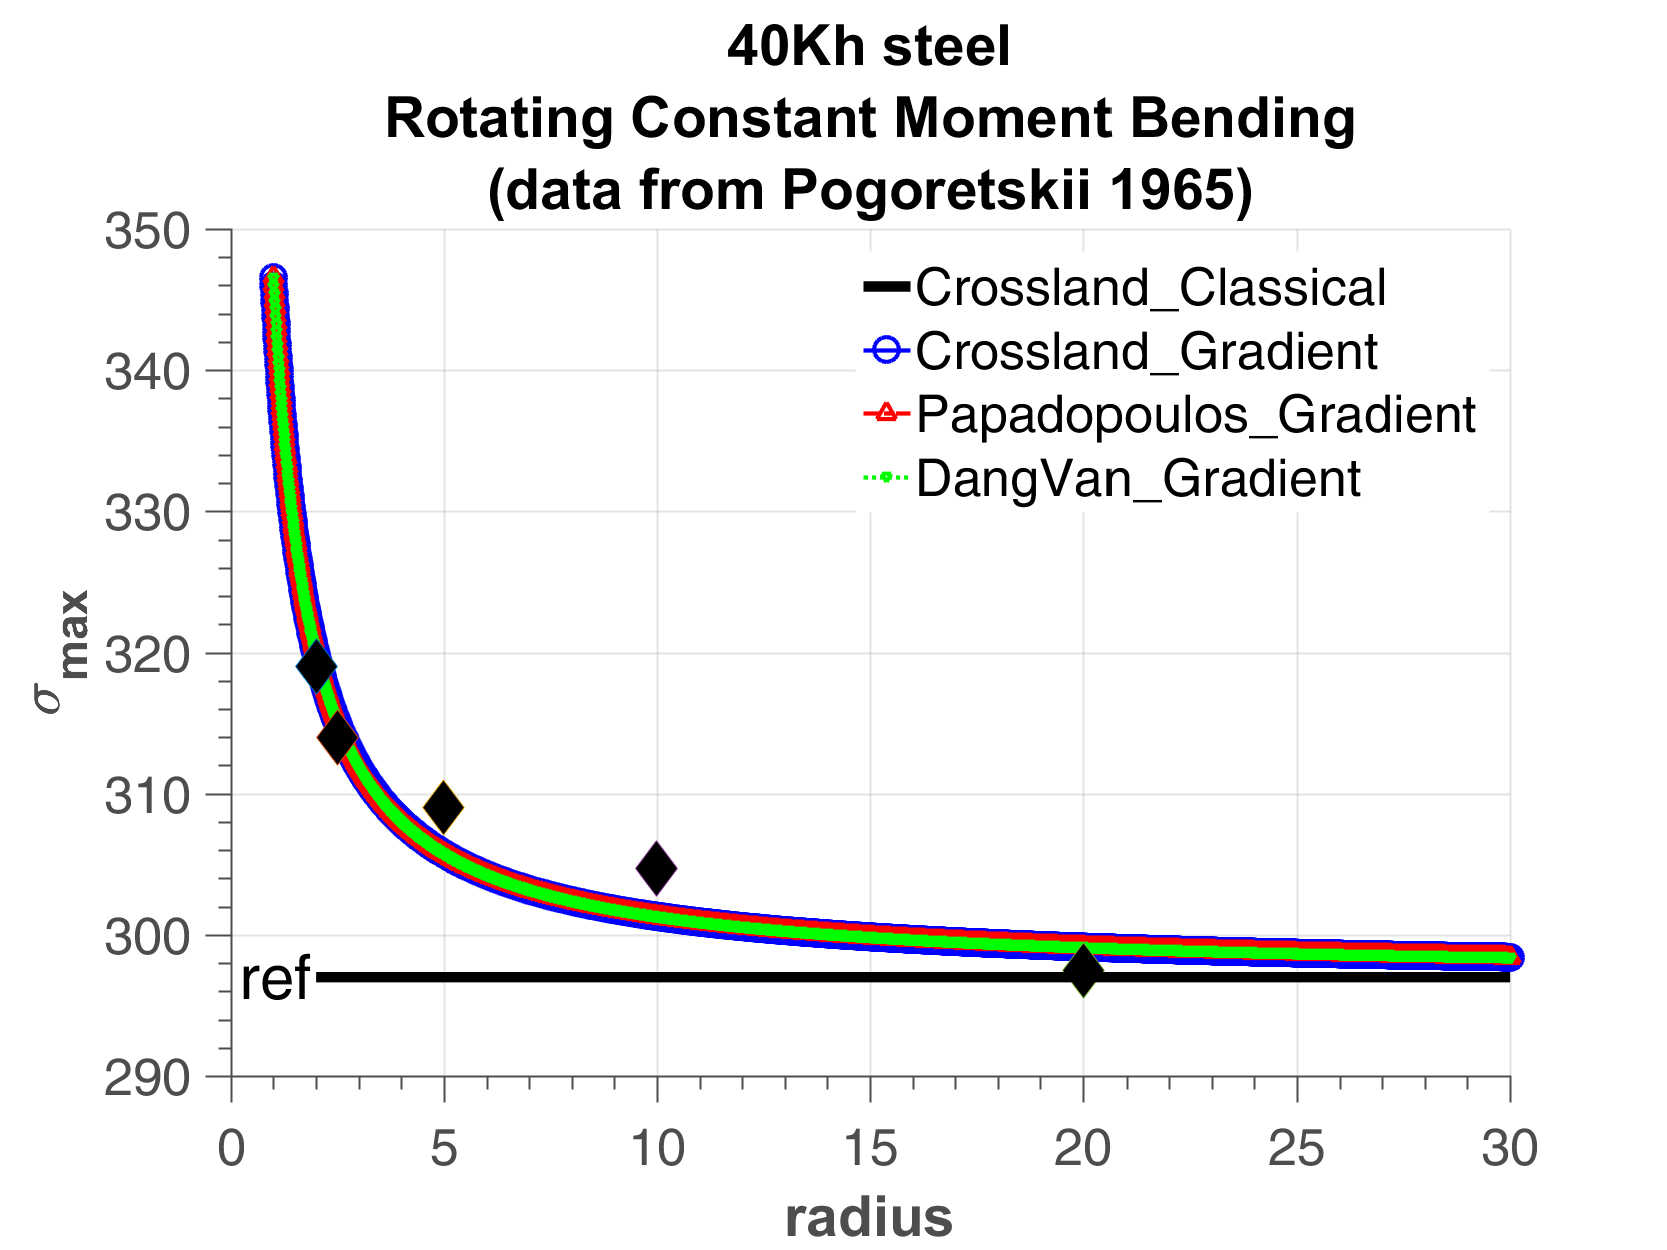
\includegraphics[width=0.9\textwidth]{figures//40khsteel.png} 
		\caption{Fatigue limits with gradient effect for different radii (\cite{Papadopoulos1996513}).}
		\label{fig.gradientcalibration4}
	\end{center}
\end{figure}
\newpage

\figref{fig.gradientcalibration1} to \figref{fig.gradientcalibration4} shows some test results of rotating bending fatigue limits
from the literature in which the fatigue limits are plotted against
the specimen radii. In the absence of gradient effect, we get the horizontal lines indicated in black. We observe that the three criteria here give very similar results when they are calibrated on uniaxial tests. \figref{fig.gradientcalibration1}, \figref{fig.gradientcalibration2} and \figref{fig.gradientcalibration3} are related to cantilever bending
tests and \figref{fig.gradientcalibration4} depicts constant moment tests.

Eq.(\ref{crossland-fr}) with $a$ et $b$ calibrated from given $S_{ref}$ and $t_{ref}$ is used to estimate the characteristic length $l_g$ in order to give the best correlation between simulated and experimental fatigue limit obtained in rotating cantilever bending tests for different materials and radii. The results are sketched and the corresponding parameters are shown in Table.\ref{tab.paras}.

\begin{table}[!h]
	\centering
	\caption{Length scales of different materials}
	\label{my-label}
	\begin{tabular}{crrrr}
		\hline
		\textbf{}                                                                   & \multicolumn{1}{c}{\textbf{1220 steel}} & \multicolumn{1}{c}{\textbf{Carbon steel}} & \multicolumn{1}{c}{\textbf{1035 steel}} & \multicolumn{1}{c}{\textbf{40Kh steel}} \\ \hline
		\textbf{\begin{tabular}[c]{@{}c@{}}$\bm{S_{ref}}$\\ {[}MPa{]}\end{tabular}} & 191                                     & 222                                       & 234                                     & 297                                     \\
		\textbf{\begin{tabular}[c]{@{}c@{}}$\bm{t_{ref}}$\\ {[}MPa{]}\end{tabular}} & 143                                     & 151                                       & 172                                     & 180                                     \\
		\textbf{\begin{tabular}[c]{@{}c@{}}$\bm{l_g}$\\ {[}mm{]}\end{tabular}}      & 0.3755                                  & 0.3297                                    & 0.2861                                  & 0.1424                                  \\ \hline
	\end{tabular}
	\label{tab.paras}
\end{table}

We can observe a very interesting phenomenon that the smaller fatigue limit is, the larger influence of gradient effect is. This phenomenon is due to the fact that the smaller the grain size, the higher the strength. This happens because of the greater interactions between dislocations as the grain size and the available room for their gliding through the lattice, is reduced. With this experimental result we can say there is positive correlations between the length scale $l_g$ and the grain size. 


\subsection{Bending-torsion fatigue tests}
\subsubsection{With Crossland criterion}
The bending moment is a linear function of $x, M_b= -F(L-x)$. The twisting moment is denoted $M_t$. The stress $\sigma_{xx}$ now varies along the depth (i.e. y-axis) and the length (i.e. x-axis) of the specimen, but as above we will neglect the gradient in $x$ as compared to the gradient in $y$. The bending stress is given here by : 
\begin{equation}
	\sigma_{a}=\dfrac{-F(L-x)}{I}R=\dfrac{M_b}{I}y \quad \text{ with } \quad I=\dfrac{\pi R^4}{4},
\end{equation}
while the twisting shear stress is given by 
$ \tau_{a}=\dfrac{M_t}{J}y \quad \text{ with  }
J=\dfrac{\pi R^4}{2}$. 
The stress tensor $\uuline{\sigma}$ is then:
\begin{equation} 
	\uuline{\sigma}(t)=
	\left(
	\begin{array}{ccc}
		\sigma_{a}sin(\omega t) & \tau_asin(\omega t) & 0\\
		\tau_asin(\omega t) & 0 & 0\\ 
		0 & 0 & 0\\
	\end{array}\right) .
\end{equation}
Its range tensor is:
\begin{equation} 
	\Delta\uuline{\sigma}=
	\left(
	\begin{array}{ccc}
		2\sigma_a& 2\tau_a & 0\\
		2\tau_a& 0 & 0\\ 
		0 & 0 & 0\\
	\end{array}\right) ,
\end{equation}
with deviator
\begin{equation} 
	\Delta\uuline{ S}=\Delta\uuline{\sigma}-\dfrac{1}{3}\textrm{tr}\Delta\uuline{\sigma}=
	\left(
	\begin{array}{ccc}
		\dfrac{4}{3}\sigma_{a} & 2\tau_a & 0\\
		2\tau_a & -\dfrac{2}{3}\sigma_a & 0\\ 
		0 & 0 & -\dfrac{2}{3}\sigma_a\\
	\end{array}\right) .
\end{equation}
The second invariant of the stress deviator is then:
\begin{equation}
	\sqrt{J_{2,a}}=\dfrac{1}{2\sqrt{2}}\sqrt{\Delta \uuline{S}:\Delta \uuline{S}}=\sqrt{\dfrac{1}{3}\sigma_a^2+\tau_a^2}=\sqrt{\dfrac{M_b^2}{3I^2}+\dfrac{M_t^2}{J^2}}y.
\end{equation}
As for the  hydrostatics stress, we have
\begin{equation}
	\sigma_{H,max}=\max\limits_{t}\left\lbrace \dfrac{1}{3}\textrm{tr}(\sigma(t))\right\rbrace =\dfrac{\sigma_{a}}{3}=\dfrac{M_b}{3I}y .
\end{equation}
Then the gradient part has the value:
\begin{equation}
	\begin{split}
		\nabla\sqrt{J_{2,a}}=\dfrac{\partial\sqrt{J_{2,a}}}{\partial x}\uline{e}_x+\dfrac{\partial\sqrt{J_{2,a}}}{\partial y}\uline{e}_y+\dfrac{\partial\sqrt{J_{2,a}}}{\partial z}\uline{e}_z=\left( 0,\sqrt{\dfrac{M_b^2}{3I^2}+\dfrac{M_t^2}{J^2}},0\right) \\=\left( 0,\dfrac{\sqrt{\frac{1}{3}\sigma_a^2+\tau_a^2}}{y},0\right) \, ,
	\end{split}
\end{equation}
and
\begin{equation}
	\nabla \sigma_{H,max}=\left( 0,\dfrac{M_b}{3I},0\right) =\left( 0,\dfrac{\sigma_a}{3y},0\right) .
\end{equation}
The parameters $a$ and $b$ of the standard Crossland criterion, are obtained from fully reversed tension-compression fatigue limit $s_{ref}$  and torsion fatigue limit $t_{ref}$ using Eq.(\ref{crossland-ab}).

\noindent From Eq.(\ref{eq:crossland}), standard Crossland criterion without gradient effect writes:
\begin{equation}
	\sqrt{J_{2,a}}+a\sigma_{H,max}=\sqrt{\dfrac{\sigma_a^2}{3}+\tau_a^2}+\dfrac{\sigma_a}{3}\leqslant b.
	\label{eqrbcross}
\end{equation}
The gradient term here is given by:
\begin{equation}
	\parallel{\nabla\sqrt{J_{2,a}}}+a{\nabla \sigma_{H,max}}\parallel= \dfrac{\sqrt{\dfrac{\sigma_a^2}{3}+\tau_a^2}}{y}+\dfrac{a\sigma_a}{3y}.
\end{equation}
Crossland criterion with beneficial gradient term as shown in Eq.(\ref{modified Crossland}) now writes
\begin{equation}
	\begin{split}
		\sqrt{J_{2,a}}+a\sigma_{H,max}-l_g\parallel{\nabla\sqrt{J_{2,a}}}+a\nabla{\sigma_{H,max}}\parallel&=\\\sqrt{\dfrac{\sigma_a^2}{3}+\tau_a^2}+\dfrac{a\sigma_a}{3}-l_g\left( \dfrac{\sqrt{\dfrac{\sigma_a^2}{3}+\tau_a^2}}{y}+\dfrac{a\sigma_a}{3y}\right) &\leqslant b.
	\end{split}
	\label{eq.arcblack}
\end{equation}
\subsubsection{With Papadopoulos criterion}
We can find the resolved shear stress $\tau(\varphi,\theta,\chi ,t)$ with Eq.\eqref{eqres}. Although the intermediate calculations are complicated, the result achieves the very simple form \cite{Papadopoulos1997219}. The generalized shear stress amplitude $T_a$ is then:
$$T_a(\varphi,\theta)=\sqrt{\dfrac{1}{\pi}\int_{x=0}^{\frac{\pi}{2}} \tau^2(\varphi,\theta,\chi)d\chi}
=\sqrt{\dfrac{\sigma_a^2}{3}+\tau_a^2}.
$$
$$\sigma_{H,max}=\dfrac{1}{3}\sigma_a$$
The modified Papadopoulos criterion from Eq.\eqref{eq:modified papa} is:
$$maxT_a+\alpha_\infty\sigma_{H,max}-l_g\parallel\nabla{maxT_a}+\alpha_\infty\sigma_{H,max}\parallel\leqslant \gamma_\infty,$$
From the above calculation and the linear dependance of the stress field as function of $y$, 
Papadopoulos criterion with beneficial gradient term reduces to 
\begin{equation}
	\begin{split}
		maxT_a+\alpha_\infty\sigma_{H,max}-l_g\parallel\nabla{maxT_a}+\alpha_\infty\sigma_{H,max}\parallel&=\\\sqrt{\dfrac{\sigma_a^2}{3}+\tau_a^2}+\dfrac{\alpha_\infty\sigma_a}{3}-l_g\left( \dfrac{\sqrt{\dfrac{\sigma_a^2}{3}+\tau_a^2}}{y}+\dfrac{\alpha_\infty\sigma_a}{3y}\right) &\leqslant \gamma_\infty.
	\end{split}
	\label{modified Papadopoulos}
\end{equation}

\subsubsection{With Dang Van criterion}
The principal stresses in 2D tensor are expressed as:
$$\sigma_1=\dfrac{\sigma_a}{2}+\sqrt{\left( \dfrac{\sigma_a}{2}\right)^2+\tau_a^2 }$$
$$\sigma_2=\dfrac{\sigma_a}{2}-\sqrt{\left( \dfrac{\sigma_a}{2}\right)^2+\tau_a^2 }$$
With this one gets the amplitude of shear stress by:
$$\max\limits_{t}\tau(t)=\dfrac{1}{2}(\sigma_1-\sigma_2)=\sqrt{\left( \dfrac{\sigma_a}{2}\right)^2+\tau_a^2 }$$
Dang Van criterion with beneficial gradient term as shown in Eq.(\ref{Dang Van}) now becomes :
\begin{equation}
	\begin{split}
		\max\limits_{t}\left\{\tau{(t)}+a_D\sigma_H(t)\right\}-l_g\parallel{\nabla\tau{(t)}}+a_D\nabla\sigma_H(t)\parallel&=
		\\\sqrt{\left(\dfrac{\sigma_a}{2}\right)^2+\tau_a^2}+\dfrac{a_D\sigma_a}{3}-l_g\left( \dfrac{\sqrt{\left(\dfrac{\sigma_a}{2}\right)^2+\tau_a^2}}{y}+\dfrac{a\sigma_a}{3y}\right) &\leqslant b_D.
	\end{split}
	\label{Dang Van}
\end{equation}

\subsubsection{Comparison with experimental data}
This classical Crossland ellipse arc delimits in the $s_{ref}-t_{ref}$  plane the safe domain against fatigue failure. In the case of fully reversed in-phase tension-compression and torsion fatigue tests, it gives the ``ellipse arc equation'' (\cite{Papadopoulos1996513}) which is Eq.\eqref{eq.arcblack} with $b=t_{ref}$ and $a=\dfrac{3t_{ref}}{s_{ref}}-\sqrt{3}$:
\begin{equation}
	\left( \dfrac{\tau_a}{t_{ref}}\right) ^2+\left( \dfrac{2s_{ref}}{\sqrt{3}t_{ref}}-1\right) \left( \dfrac{\sigma_a}{s_{ref}}\right) ^2+\left( 2-\dfrac{2s_{ref}}{\sqrt{3}t_{ref}}\right) \dfrac{\sigma_a}{s_{ref}}\leqslant 1
	\label{crossland}
\end{equation}

However, if one tries to predict the behavior of the material in combined bending and torsion, which involves  the gradients of normal and shear stresses, high discrepancies between predictions and experimental data will be found. 

By introducing the values of $\sqrt{J_{2,a}}$ and $\sigma_{H,max}$ in the the classical Crossland criterion, along with the change of parameter $a$  from $\left(\dfrac{3 t_{-1}}{s_{-1}}-\sqrt{3}\right)$ to $\left(\dfrac{3 t_{-1}}{f_{-1}}-\sqrt{3}\right)$ in Eq.\eqref{eq:crossland}, we obtain the ``Papadopoulos ellipse arc" based on $\left(t_{-1},f_{-1} \right) $ in the plane of amplitudes $\sigma_a$ and $\tau_a$:
\begin{equation}
	\left(\dfrac{\tau_a}{t_{-1}}\right)^2+\left(\dfrac{2f_{-1}}{\sqrt{3}t_{-1}}-1\right)\left(\dfrac{\sigma_a}{f_{-1}}\right)^2+\left(2-\dfrac{2f_{-1}}{\sqrt{3}t_{-1}}\right)\dfrac{\sigma_a}{f_{-1}}\leqslant 1
	\label{papa}
\end{equation}
This apparent size effect, which is actually a gradient effect, in taken
into account intrinsically by gradient fatigue criteria, as for instance
proposed in \cite{Papadopoulos1996513}. Nevertheless, these criteria do not take into account the possible dependence of the fatigue limit on the shear
stress gradient and consequently do not distinguish between $t_{-1}$
and $t_{ref}$.

It can be seen from \figref{4340} that the Crossland ellipse arc (Eq. \ref{crossland}) based on the $s_{ref}$-$ t_{ref}$ fatigue limits and the Crossland ellipse arc (Eq. \ref{papa}) based on $f_{-1}$-$t_{-1}$ are different demonstrating clearly the effect of stress gradient. The first curve, obtained within zero normal stress gradient assumption, does not fit the experimental data from combined bending-twisting tests having a non-zero stress gradient.  The difference between test points and classical Crossland ellipse arc near the x-axis where the normal load is predominant, is a proof of the beneficial ``size’’ and gradient effects. Indeed, the difference between two kinds of fatigue test can be clearly seen: the bending test (test points) includes the beneficial effects of the normal stress gradient; the tension–compression test (Crossland ellipse arc) excludes these effects due to the gradient-free stress state.  To account for the shear gradient amplitude effect, a clear distinction must be made between $t_{ref}$
determined at the radius $R_{\infty}$ of specimen large enough and $t_{-1}$ determined at the radius $R$ of the considered specimen.
Then all
these above analyses affirm, first, the ``size effect'' on fatigue limits
(Smaller is Stronger) as well as the beneficial effect of the normal
stress gradient (Higher Gradient is Stronger), and second, the
necessity of a distinction between $t_{ref}=t(R_{\infty})$ and $t_{-1}(R)$ when applied to the classical Crossland criterion and the new gradient criterion, respectively. With all such conceptions, the experimental data now agree very well with the ellipse arc based on  the new criteria proposed, as plotted in \figref{4340}. It is also noticed that the substitution of the material parameters by the bending and torsion limits is an unorthodox way to bypass the above described problems for classical criterion. The same ellipse arc is obtained in a more intrinsic way using the proposed criterion.

Our proposal takes into account both gradients of hydrostatic stress and shear stress. For SAE 4340 steel, the tension-compression fatigue limit $S_{ref}=397MPa$ and the torsion fatigue limit $t_{ref}=258MPa$. We use the same set of parameters as the original criteria except the gradient term with length scale $l_g$. Choosing the proper $l_g$(here $l_g=2.5mm$ ) allows us to predict the experiments within the acceptable range as shown in \figref{4340} at the critical locations $y=R$. These results, represented in the $\sigma_a, \tau_a$ plane (the so called fatigue ellipse arc)  illustrate that our proposal is quite satisfactory in biaxial case.	

\begin{figure}[!h]
	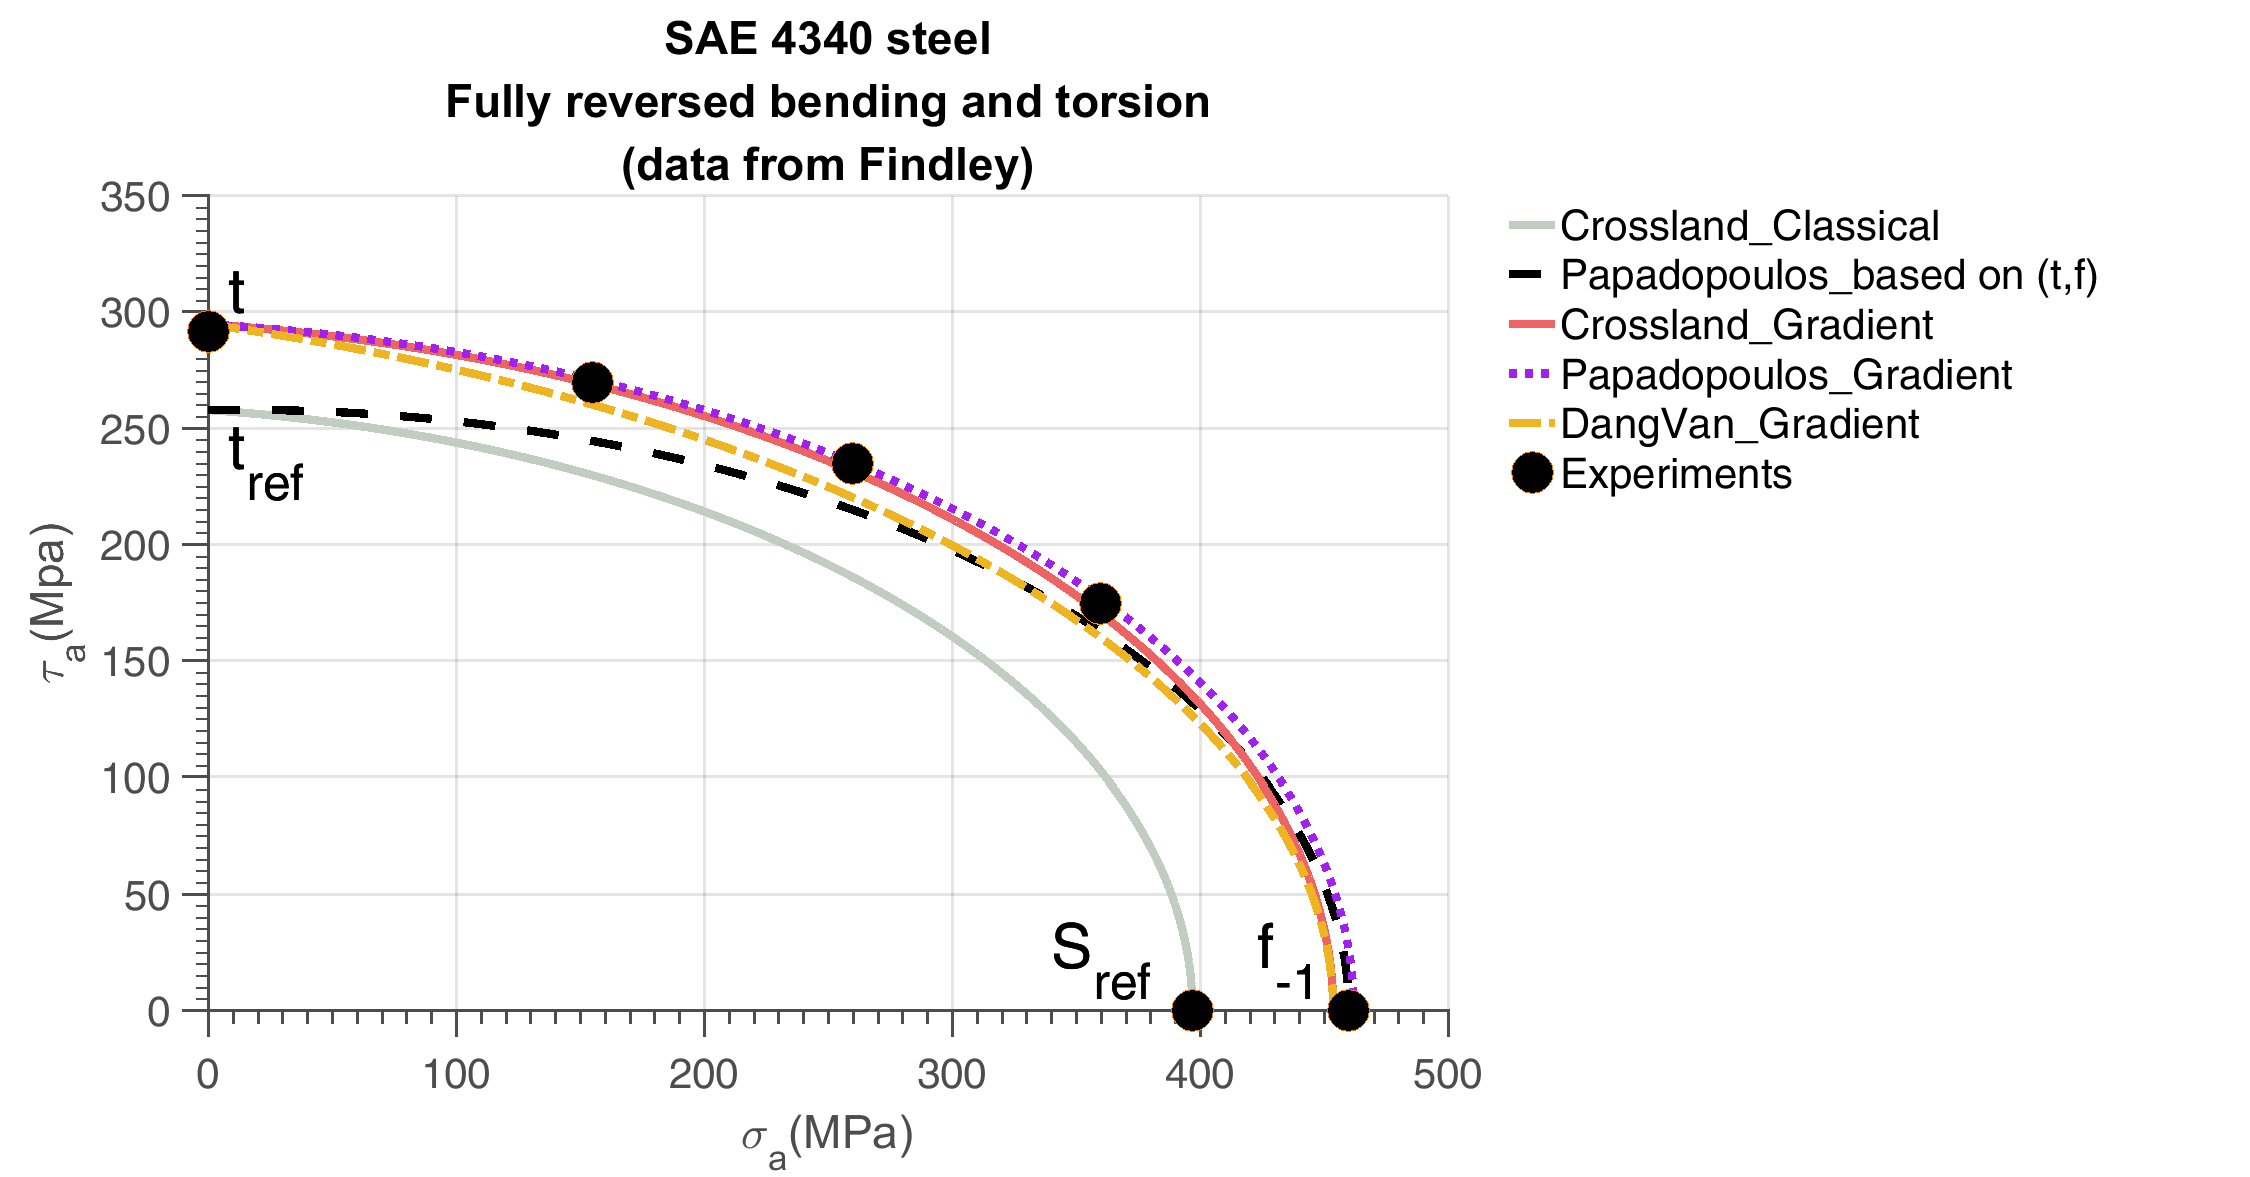
\includegraphics[width=\textwidth]{figures//4340.png}
	\caption{Fully reversed combined bending-twisting fatigue limit data (\cite{findley1956theory}, \cite{Papadopoulos1996513}) compared with updated values computed with gradient effects using 	Eq.\ref{eq.arcblack}, Eq.\ref{modified Papadopoulos}, Eq.\ref{Dang Van}, Eq.\ref{crossland} and Eq.\ref{papa} with $l_g = 2.5 \, mm$. In absence of gradient effect, we would get the inner gray ellipse corresponding to classical Crossland criterion.}
	\label{4340}
\end{figure}



\newpage
\section{Discussion}
\noindent\textbf{Remark 1} (Gradient terms). In this work, the pure size effect has not been considered and only stress gradient effect is modeled. Whereas the latter is dominant rather than totally to the pure size effect as usually believed. 
A unique gradient term is enough to model the gradient and loading effects. This is introduced either in the normal stress component of the classical fatigue criterion as \cite{Papadopoulos1996513} proposed, or in the shear stress part as presented in \cite{Massonnet1956}. However, in multiaxial fatigue tests, combining two types of stress gradient terms is in principle indispensable to capture the previous effects.
\vspace{6pt} \\
\textbf{Remark 2} (Material characteristic length scale $l_g$). The values of $l_g$ of the model proposed extend from
several hundredths of a micron to about a millimeter for cases considered, while the one of the model
proposed very recently by  \cite{Ferre201356} takes about a micron. The very difference between them
is physically explained by the following reason: we study here the fatigue endurance of macroscopic
specimens and components for which the crack initiation is generally detected by loss of stiffness corresponding to crack length which can reach a millimeter; whereas Ferr{\'e} et al. consider crack nucleation in
the scale is few dozen microns.
\vspace{6pt} \\
\textbf{Remark 3} (Extensions to other load case). The dependence of fatigue limits on both ``size" and gradient effects according to the specimen size (e.g. length,radius) has a ``saturated" or ``insensitive" threshold. That
means, there always exists a certain ``saturated" value for the specimen size ($L\infty$ ,$R\infty$ ) from which the
fatigue behavior is insensitive to both effects and the proposed criteria exactly reduce to the respective
classical ones. Nevertheless, it is not easy to compute the gradient in multiaxial loading case.

\section{Conclusion and perspectives}

The present work develops a simple formulation of gradient multiaxial fatigue criteria extending the
classical HCF criteria. The objective is to model the ``size", surface gradient and loading effects, not
included yet in classical mechanics but become important at small scale, by taking into account just the
gradient effect. Basing on some experimental observations, and departing from classical fatigue criteria, new class of
criteria with stress gradient terms entering not only in the normal stress but also in the shear stress
amplitude, are proposed. Such a formulation allows the new criteria to capture the ``size" and gradient
effects, and to cover a large range of loading mode (traction, bending, shearing). These new criteria
are then generalized to multiaxial cases to capture both well-known phenomena ``Smaller is Stronger"
and ``Higher Gradient is Stronger" and thus can reproduce fatigue experimental data even at small scale.
Here in this work, the nature of these two phenomena is also clarified. "Higher Gradient is Stronger" is
only related to the gradient effect, while "Smaller is Stronger" is related to both pure size and gradient
effects where the latter is dominant - rather than totally to the pure size effect as usually believed.
Extensions of some classical fatigue limit criteria such Crossland and Dang Van are done as illustrations.
The proposed criteria shown a good agreement with a number of experiments from the literature. A
more comprehensive introduction of a practical strategy to compute local gradient and validation  for complex loading (real multiaxial loads) could be perspective for this
research direction. 

In methodological aspect, gradient approach just allow modeling the volumetric stresses instant distribution (related to loading case such as: tension-compression, torsion, plane bending), not volumetric stresses distribution all over the loading cycle (related to rotative bending). Thus the adopted criteria indifferently deal with the plane bending and the rotative bending tests, although their fatigue limits are actually different. Fatigue problems concerning other factors (machining, notches, defects, inclusions, corrosion, etc.) have been left out in this approach and need another approach to address. In particular for notched fatigue problems, this approach may be still applicable. A validation by means of experimental data is needed to examine this possibility. Cases with critical points located inside specimens where the gradient effect can be presumably negative on fatigue resistance, for instance those with presence of residual stresses, can be encountered and have not examined yet. A reexamination of the approach will be the object of the further work. % Results and Discussion
%!TEX root=../Thesis_Zepeng.tex
\chapter{Time varying load : the standard approach}\label{chp:4}
\minitoc
%Fatigue failure is a damage accumulation process in which material property deteriorates continuously under
%fatigue loading and the damage depends on the size of
%stress and strain. With the accumulation of fatigue
%damage, some accidents occur for these components. Research shows that a reliable lifetime prediction method is
%particularly important in the design, safety assessments,
%and optimization of engineering components and structures. Thus, it is important to formulate an accurate method
%to evaluate the fatigue damage accumulation and effectively predict the fatigue life of these components.
%The objective of this work is to contribute to the development life model that take into account the presence of complex variations of the stress tensor. We focus on Chaboche damage accumulation law in case of multiaxial high cycle fatigue. Heuristic formulations with different multiaxial fatigue criteria have been proposed. 

\section{The notion of damage in fatigue}


In the case of fatigue, we usually employ the concept of the loading cycle instead of time to evaluate the evolution of damage and to measure the fatigue lifetime. The equations then depend on the load through globally defined quantities over a cycle, such as amplitude, maximum value, mean value.
The growth equation of fatigue damage is therefore taken in the form:
$$\delta D=f(D)\delta N$$
$$\delta N=f_n\delta t$$
where $\delta t$ is a time sampling of the history in a given number of time intervals $\delta t_1,\delta t_2 ... \delta t_i, ...$ and $f_n$ is the mean frequency of those cycles during the considered time step. The issue is thus to identify the function $f(D,S_a,S_m)$ relating the damage growth to the present damage, the load amplitude, the load mean value and so on. We will focus in this chapter on the classical ways of taking into account a possible dependence on $D$.

\subsection{Linear and nonlinear accumulation of damage}
Cumulative effects, whether linear or nonlinear, are of great importance in fatigue. The rule of linear accumulation is in fact a property of any linear or nonlinear differential equation with separable variables. One approach to variable load histories uses the concept of fraction of life(also referred to as cycle ratio) used up by an event. These fractions are added together; when their sum reaches 1.0 or 100 percent we expect failure. This is the most common measure of damage, and is the quantifying measure we present here. 

The Palmgren-Miner linear rule as explained in \cite{lemaitre1990mechanics} is based on the assumption that damage is accumulated additively when it is defined by the associated life ratio $N_i/N_{Fi}$ where $N_i$ is the number of cycles applied under a given load for which the number of cycles to fracture(under periodic conditions) would be $N_{Fi}$. The fracture criterion is:
$$\sum_{i}N_i/N_{F_i}=1.$$
Therefore, in periodic tests, damage evolution is considered to be linear in that:
$$D=N/N_F.$$
For a test at two stress levels, the evolution is as shown schematically in \figref{linear accumulation}. In fact, the linear accumulation rule can be applied even to a damage which evolves nonlinearly. For this it is sufficient that a one-to-one relationship between $D$ and $N/N_F$ exists, or even that the damage evolution curve be a unique function(independent of the applied cycle) of the life ratio $N/N_F$ . 

There are, therefore, two ways of defining a damage incremental law incorporating the linear accumulation rule. It can be linear of the form and shown in \figref{linearevolution}:
$$\delta D= \delta N/N_F(...),$$
\begin{figure}[!h]
	\centering
	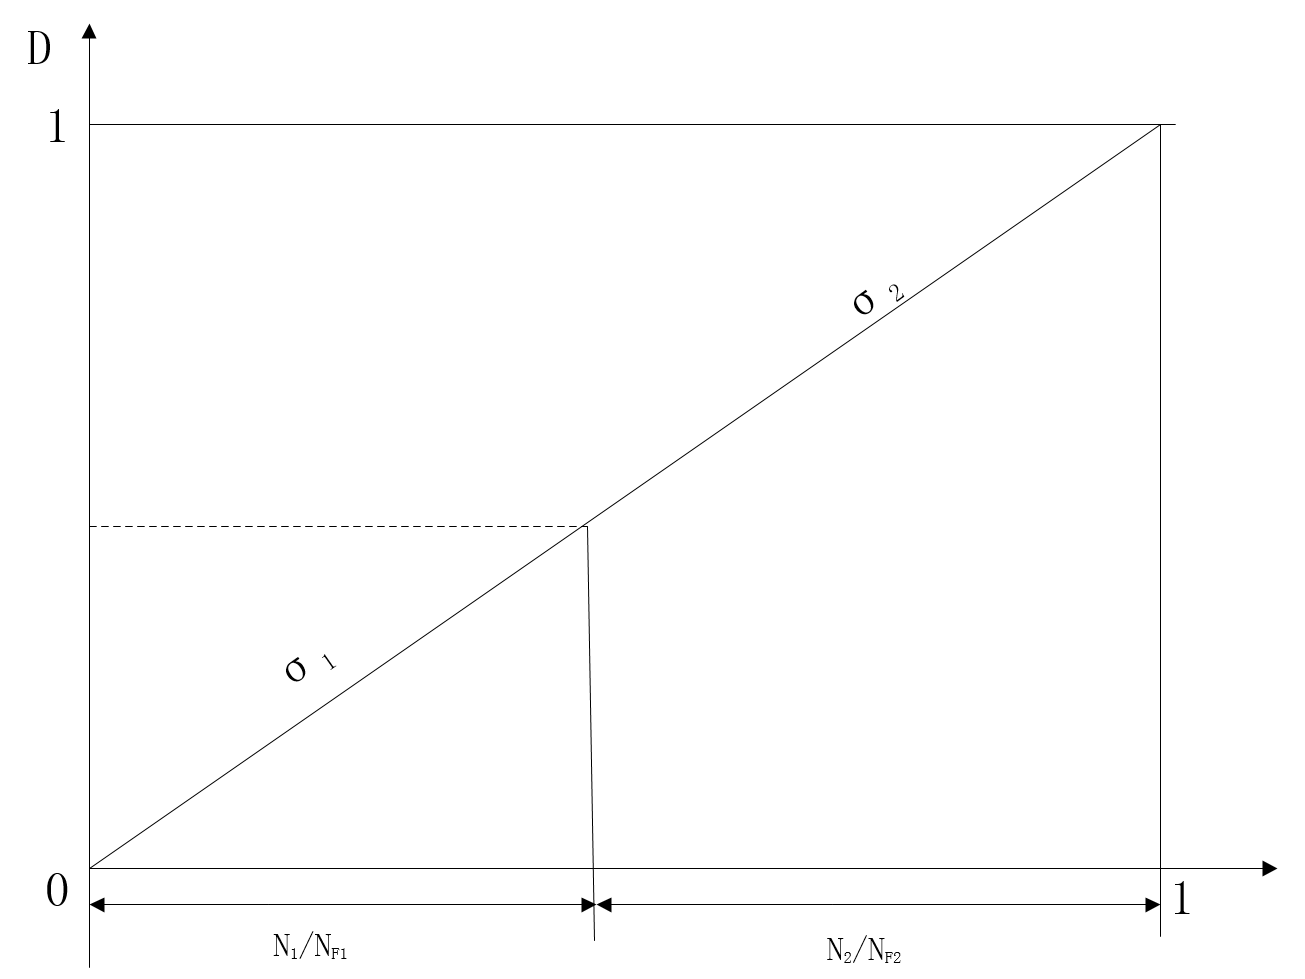
\includegraphics[width=0.8\textwidth]{figures//linearevolution.png} 
	\caption{Linear accumulation of damage with linear evolution}
	\label{linearevolution}
\end{figure}
where $N_F$ is the number of cycles to failure defined by the chosen parametric data.
The damage evolution can be nonlinear such as:
$$\delta D= \frac{(1-D)^{-k}}{k+1}\frac{\delta N}{N_F(...)}.$$
Here in any case, the damage evolution curve as function of life ratio $\delta N/N_F$ is supposed to be independent of the local state of stress (\figref{linear accumulation}).
\begin{figure}[!h]
	\centering
	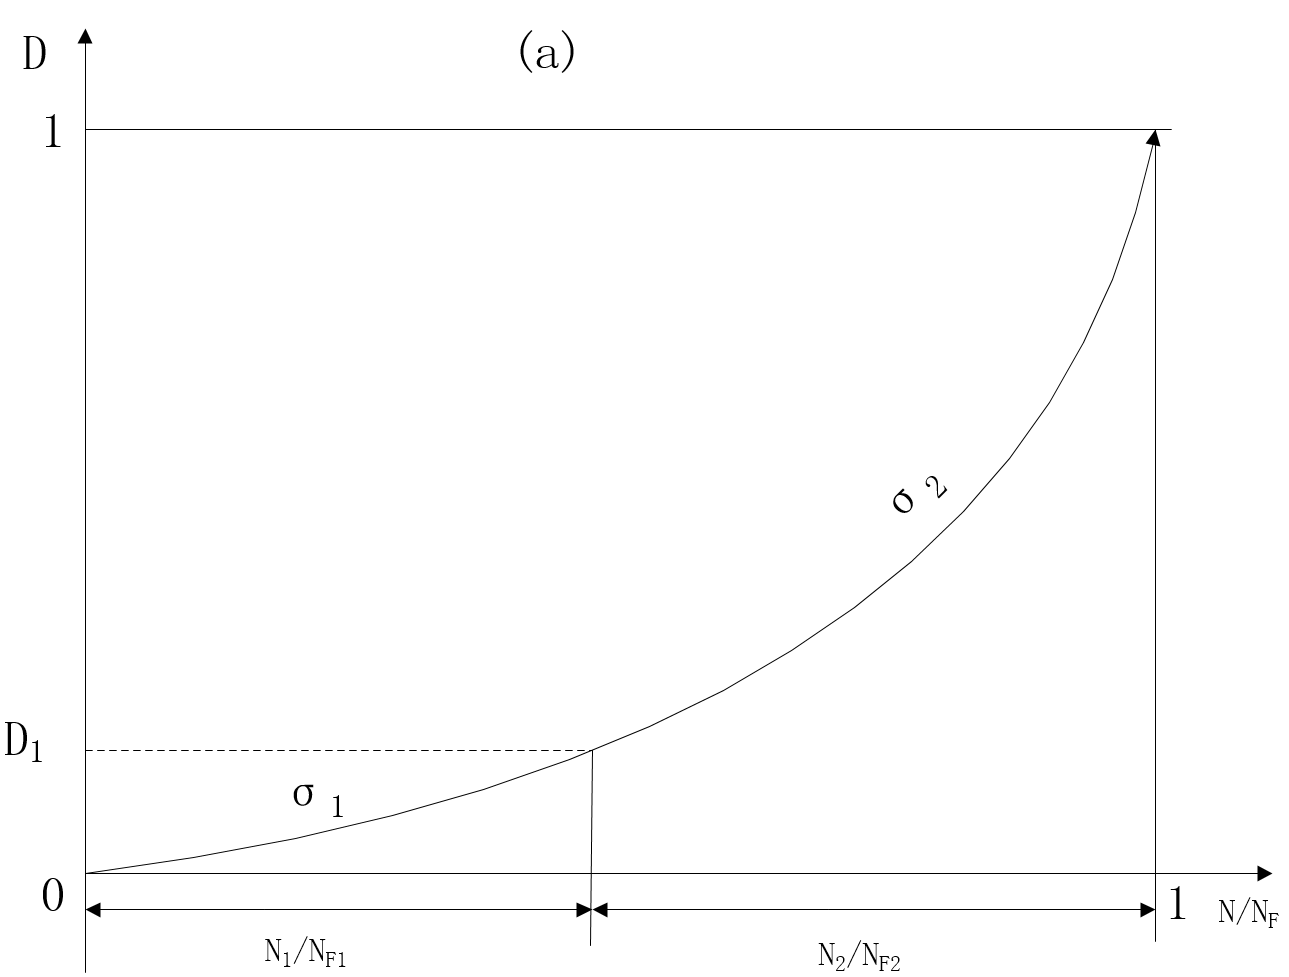
\includegraphics[width=0.8\textwidth]{figures//linearaccumulation.png} 
	\caption{Damage with nonlinear evolution and linear accumulation, where high then low stress loading sequence leads to the same fatigue life.}
	\label{linear accumulation}
\end{figure}
In contrast, if the damage evolution curve,as a function of the life ratio $N/N_F$, depends on the applied loading we have the effect of nonlinear accumulation as shown in \figref{nonlinear accumulation}. 
\begin{figure}[!h]
	\centering
	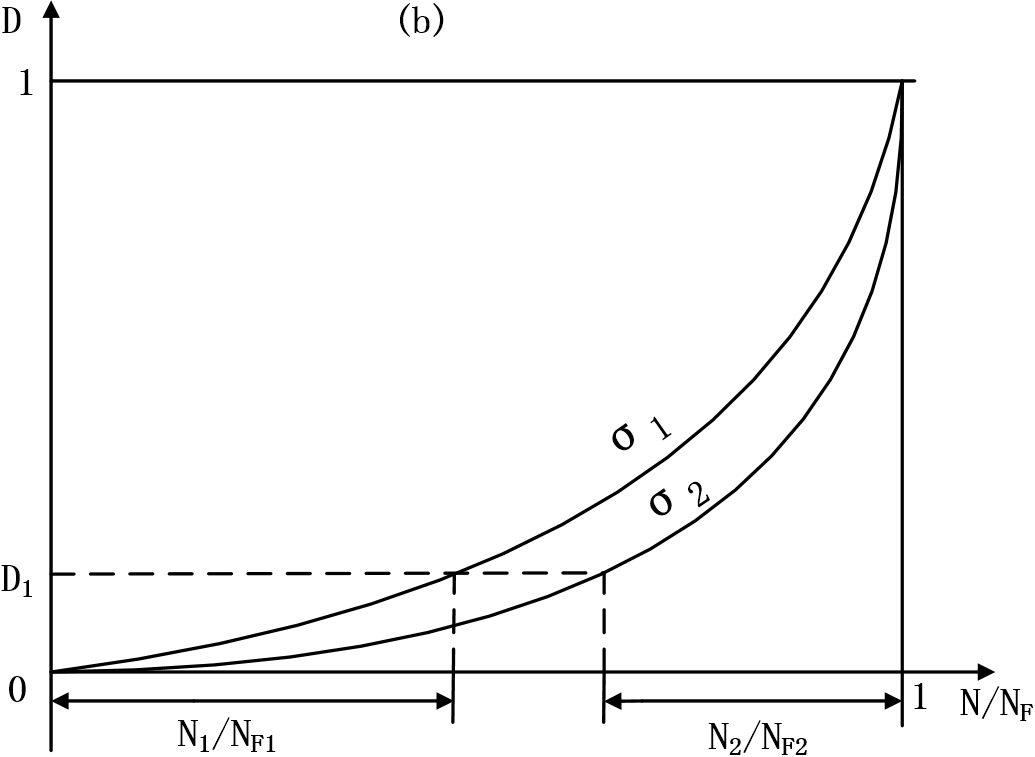
\includegraphics[width=0.8\textwidth]{figures//nonlinearaccumulation.png} 
	\caption{Damage with nonlinear evolution and nonlinear accumulation, where high stress and low stress follow different damage evolution curve. This leads to the summation of fatigue life proportion difference between different loading sequence.}
	\label{nonlinear accumulation}
\end{figure}
There, $D_1$ represents the state of internal damage at the end of the first level $\sigma_1$. Evolution at the second level $\sigma_2$ continues from the same state, and it is clear that the sum of the life ratio is less than 1. From the point of view of the damage law, this nonlinearity always corresponds to the case where the variables which represent the load $\sigma$ and the damage variable $D$ have coupled evolution.

The Palmgren-Miner linear accumulation law gives good results only for loads for which there is little variation in the amplitude and mean value of stress. The assumption of linear damage is open to many objections. For example, sequence and interaction of events may have major influences on life, the rate of damage accumulation may depend on the load amplitude, experimental evidence often indicates that $\sum_{i}N_i/N_{F_i}\neq 1$ for a low-to-high or a high-to-low loading sequence, all effects which are not taken into account in the linear damage assumption.

\newpage
\subsection{Classic Chaboche damage law}

In cyclic loading, one way of writing a damage law which expresses the experimental results is to assume that the damage per cycle is a function of the maximum and the mean values of the stress:
$$\delta D/\delta N=f(\sigma_{Max},\sigma_m).$$
In order to recover, after integration, one of the many forms proposed to represent the Wohler curves, Chaboche proposes to use a law such as:
\begin{equation}
\delta D/\delta N=\frac{\sigma_{Max}-\sigma_l(\sigma_m)}{\sigma_{u}-\sigma_{Max}}\left( \frac{\sigma_{Max}-\sigma_m}{B(\sigma_m)}\right) ^{\gamma}.
\label{generalchaboche}
\end{equation}
with:

$\sigma_l(\sigma_m)=\sigma_m+s_{-1}(1-b\sigma_m)$ :  fatigue limit.

$B(\sigma_m)=B_0(1-b\sigma_m)$ : the mean stress component in the fatigue limit.

$\sigma_u$ : ultimate stress of the material.

The number of cycles to failure is obtained by an obvious integration, with the condition:

$N=0 \to D=0$(initial undamaged state)

$N=N_F \to D=1$(macro-crack initiation)

so that by integration Eq.\eqref{generalchaboche} from $D=0$ to $D=1$ we get:
\begin{equation}N_F=\frac{\sigma_{u}-\sigma_{Max}}{\sigma_{Max}-\sigma_l(\sigma_m)}\left(\frac{\sigma_{Max}-\sigma_m}{B(\sigma_m)}\right)^{-\gamma}.
\label{NF}
\end{equation}

Eq.\eqref{generalchaboche} then writes:
$$\delta D=\delta N/N_F.$$

The constants are determined from conventional data:$\sigma_u$ is usually known, $s_{-1},b$ fit the results on the fatigue limits with relation $\sigma_l(\sigma_m)=\sigma_m+s_{-1}(1-b\sigma_m)$. Exponent $\gamma$ is obtained from the S-N curve for reversed conditions, by plotting $\sigma_{Max}$ as function of $N_F(\sigma_{Max}-\sigma_l(\sigma_m))/(\sigma_{u}-\sigma_{Max})$, as deduced from Eq.\eqref{NF}. Coefficient $B(\sigma_m)$ is obtained from one point of the S-N curve.

\vspace{6pt}
\textbf{Uniaxial case}
\vspace{6pt}

The equation studied below allows us to describe the effects of nonlinear accumulation in the case of non-periodic cyclic loads\cite{FFE:FFE1}. A simple way to introduce such effects in the damage growth equation consists in rendering the load and damage variables non-separable. For example, we may take:
$$\delta D=D^{\alpha(\sigma_{Max},\sigma_m)}\left(\frac{\sigma_{Max}-\sigma_m}{B(\sigma_m)}\right)^\gamma\delta N$$
The exponent $\alpha$ depends on the loading $(\sigma_{Max},\sigma_m)$, which results in non-separability. A reference choice is

\vspace{6pt}
$$\alpha(\sigma_{Max},\sigma_m)=1-a\left\langle\dfrac{\sigma_{Max}-\sigma_l(\sigma_m)}{\sigma_u-\sigma_{Max}}\right\rangle$$
\vspace{6pt}

The exponent $\alpha$ represents the effect of the internal variables(for example the hardening state of the material), which depends on the loading $(\sigma_{Max},\sigma_m)$, resulting in non-separability. It induces allows a non-linear damage cumulative rule as it is experimentally observed above. $a$ and $\gamma$ are material parameters. The coefficients $\gamma$ is determined from experimental Woehler's curves. 

The concept of effective stress applied to fatigue provides an indirect measure. The measured evolutions are extremely nonlinear. With this concept, damage can really be measured only in the last part of the life-time, when microscopic initiations have already occurred(this is the phase of micro-propagation of defects). And these damage evolutions are extremely nonlinear. To reproduce this phenomenological aspect it is sufficient to make a change of variable by replacing $D$ in the previous equation by:
$$1-(1-D)^{\gamma+1}.$$
The differential law can be written as:
\begin{equation}\delta D=[1-(1-D)^{\gamma+1}]^{\alpha(\sigma_{Max},\sigma_m)}\big[\frac{\sigma_{Max}-\sigma_m}{M(\sigma_m)}\big]^\gamma\delta N
\label{diff}
\end{equation}

This form is more complex, but its properties are identical to the properties of the previous equation, except for the current value of damage. Now we integrate it to see how damage $D$ evolves with cycle numbers $N$ and the influence of different parameters. By differential calculus, we get from Eq.\eqref{diff}:
\begin{equation}\delta [1-(1-D)^{\gamma+1}]^{1-\alpha}=(1-\alpha)(\gamma+1)\big[\frac{\sigma_{Max}-\sigma_m}{M(\sigma_m)}\big]^\gamma\delta N.
\label{easyintegration}
\end{equation}


The number of cycles to failure, obtained by integrating $D$ from 0 to 1 is thus:
\begin{equation}N_F=\frac{1}{(\gamma+1)(1-\alpha)}\left(\frac{\sigma_{Max}-\sigma_m}{M(\sigma_m)}\right)^{-\gamma}
\label{eqnf}
\end{equation}
and we find by comparing with Eq.\eqref{NF} that $M(\sigma_m)=B(\sigma_m)(\gamma+1)^{1/\gamma}$. This form Eq.\eqref{eqnf} can be used in experimental Woehler's curve in order to identify the coefficient $a$ and $\gamma$. In differential form,  from Eq.\eqref{easyintegration} and Eq.\eqref{eqnf}, we get equivalently
\begin{equation}\delta [1-(1-D)^{\gamma+1}]^{1-\alpha}=\frac{\delta N}{N_F}
\label{diffform}
\end{equation}
When we integrate Eq.\eqref{easyintegration} from $0$ to $D$ at constant loading conditions. The damage, expressed as a function of $N/N_F$ is:
\begin{equation}D=1-\left[ 1-\left( \frac{N}{N_F}\right) ^{\frac{1}{1-\alpha}}\right] ^{\frac{1}{\gamma+1}}.
\end{equation}
This expression is in good agreement with experimental results\cite{lemaitre1990mechanics}. 

\vspace{6pt}
\textbf{Multiaxial case}
\vspace{6pt}

The applied stress and strain tensors are often multiaxial and present a complex path during a loading cycle. In the case of multiaxial loading fatigue, the Chaboche model is represented by the following equation:
\begin{equation}\delta D = \left( 1 -(1-D)^{\gamma+1}\right)^\alpha \left(\frac{\widetilde{A}_{\uppercase\expandafter{\romannumeral2}}}{M(\sigma_H)}\right)^\gamma \delta N
\label{chabochemulti}
\end{equation} 
where the amplitude $\sigma_{Max}-\sigma_l(\sigma_m)$ is replaced by the deviatoric norm $A_{\uppercase\expandafter{\romannumeral2}}$ and the average stress is replaced by the hydrostatic pressure. We should note that for an isotropic damage theory, we will have from Eq.\eqref{easyintegration}
$$\widetilde{A}_{\uppercase\expandafter{\romannumeral2}}=A_{\uppercase\expandafter{\romannumeral2}}/(1-D)$$

\begin{equation}\alpha = 1 - a\left\langle \frac{A_{\uppercase\expandafter{\romannumeral2}} - A_{\uppercase\expandafter{\romannumeral2}}^\ast(\sigma_H)}{ \sigma_{u} - \sigma_{eqMax}}\right\rangle.\end{equation}

Again, $\alpha$ represents the influence of internal variables,characterizes the non-linearity of the damage evolution, allows to take into account the mean stress effect and describes the damage occurrence of the material: as long as $\alpha < 1$, there is damage creation. The coefficient $a$ gives the amount of fragility which is induced by a given occurrence of fatigue limit violation.

In this formula, $A_{\uppercase\expandafter{\romannumeral2}}$ is the amplitude of octahedral shear stress given by:

\begin{equation}A_{\uppercase\expandafter{\romannumeral2}}=\frac{1}{2}\max\limits_{t}\sqrt{\frac{1}{2}\uline{\uline{\Delta s}}:\uline{\uline{\Delta s}}}=\sqrt{J_2}_a=\frac{1}{2}\Delta\sigma_{eqmax},\end{equation}

The quantity $A_{\uppercase\expandafter{\romannumeral2}}^\ast(\sigma_H)$ represents the infinite life fatigue limit. For example,the Sines fatigue limit criterion is formulated by the following equation:
\begin{equation} A_{\uppercase\expandafter{\romannumeral2}}^\ast(\sigma_H)=s_{-1}(1-3b\sigma_H).\end{equation}

Above, $s_{-1}$ and $\sigma_{u}$ are respectively the fatigue limit at zero mean stress and the ultimate tensile stress. For steel, we usually have $s_{-1}\approx 0.48\sigma_{u}$.

The function $M(\sigma_H)$ in Eq.\eqref{chabochemulti} quantifies the mean stress effect through Low Cycle Fatigue(LCF) loading range:
$$M(\sigma_H)=s_{-1}\left(1-3\frac{\sigma_H}{\sigma_u}\right).$$

We can get the $D-N$ curve in \figref{DN} by integrating Eq.\eqref{chabochemulti}. This is in the case of constant loading conditions because we regard $\alpha$ and $\gamma$ as invariable parameters.
\begin{equation}N =\frac{( 1 -(1-D)^{\gamma+1})^{1-\alpha}}{(1+\gamma)(1-\alpha)}\left[\frac{A_{\uppercase\expandafter{\romannumeral2}}}{M(\sigma_H)}\right]^{-\gamma} 
\label{D-N}
\end{equation} 

\begin{figure}[h!]
	\centering
	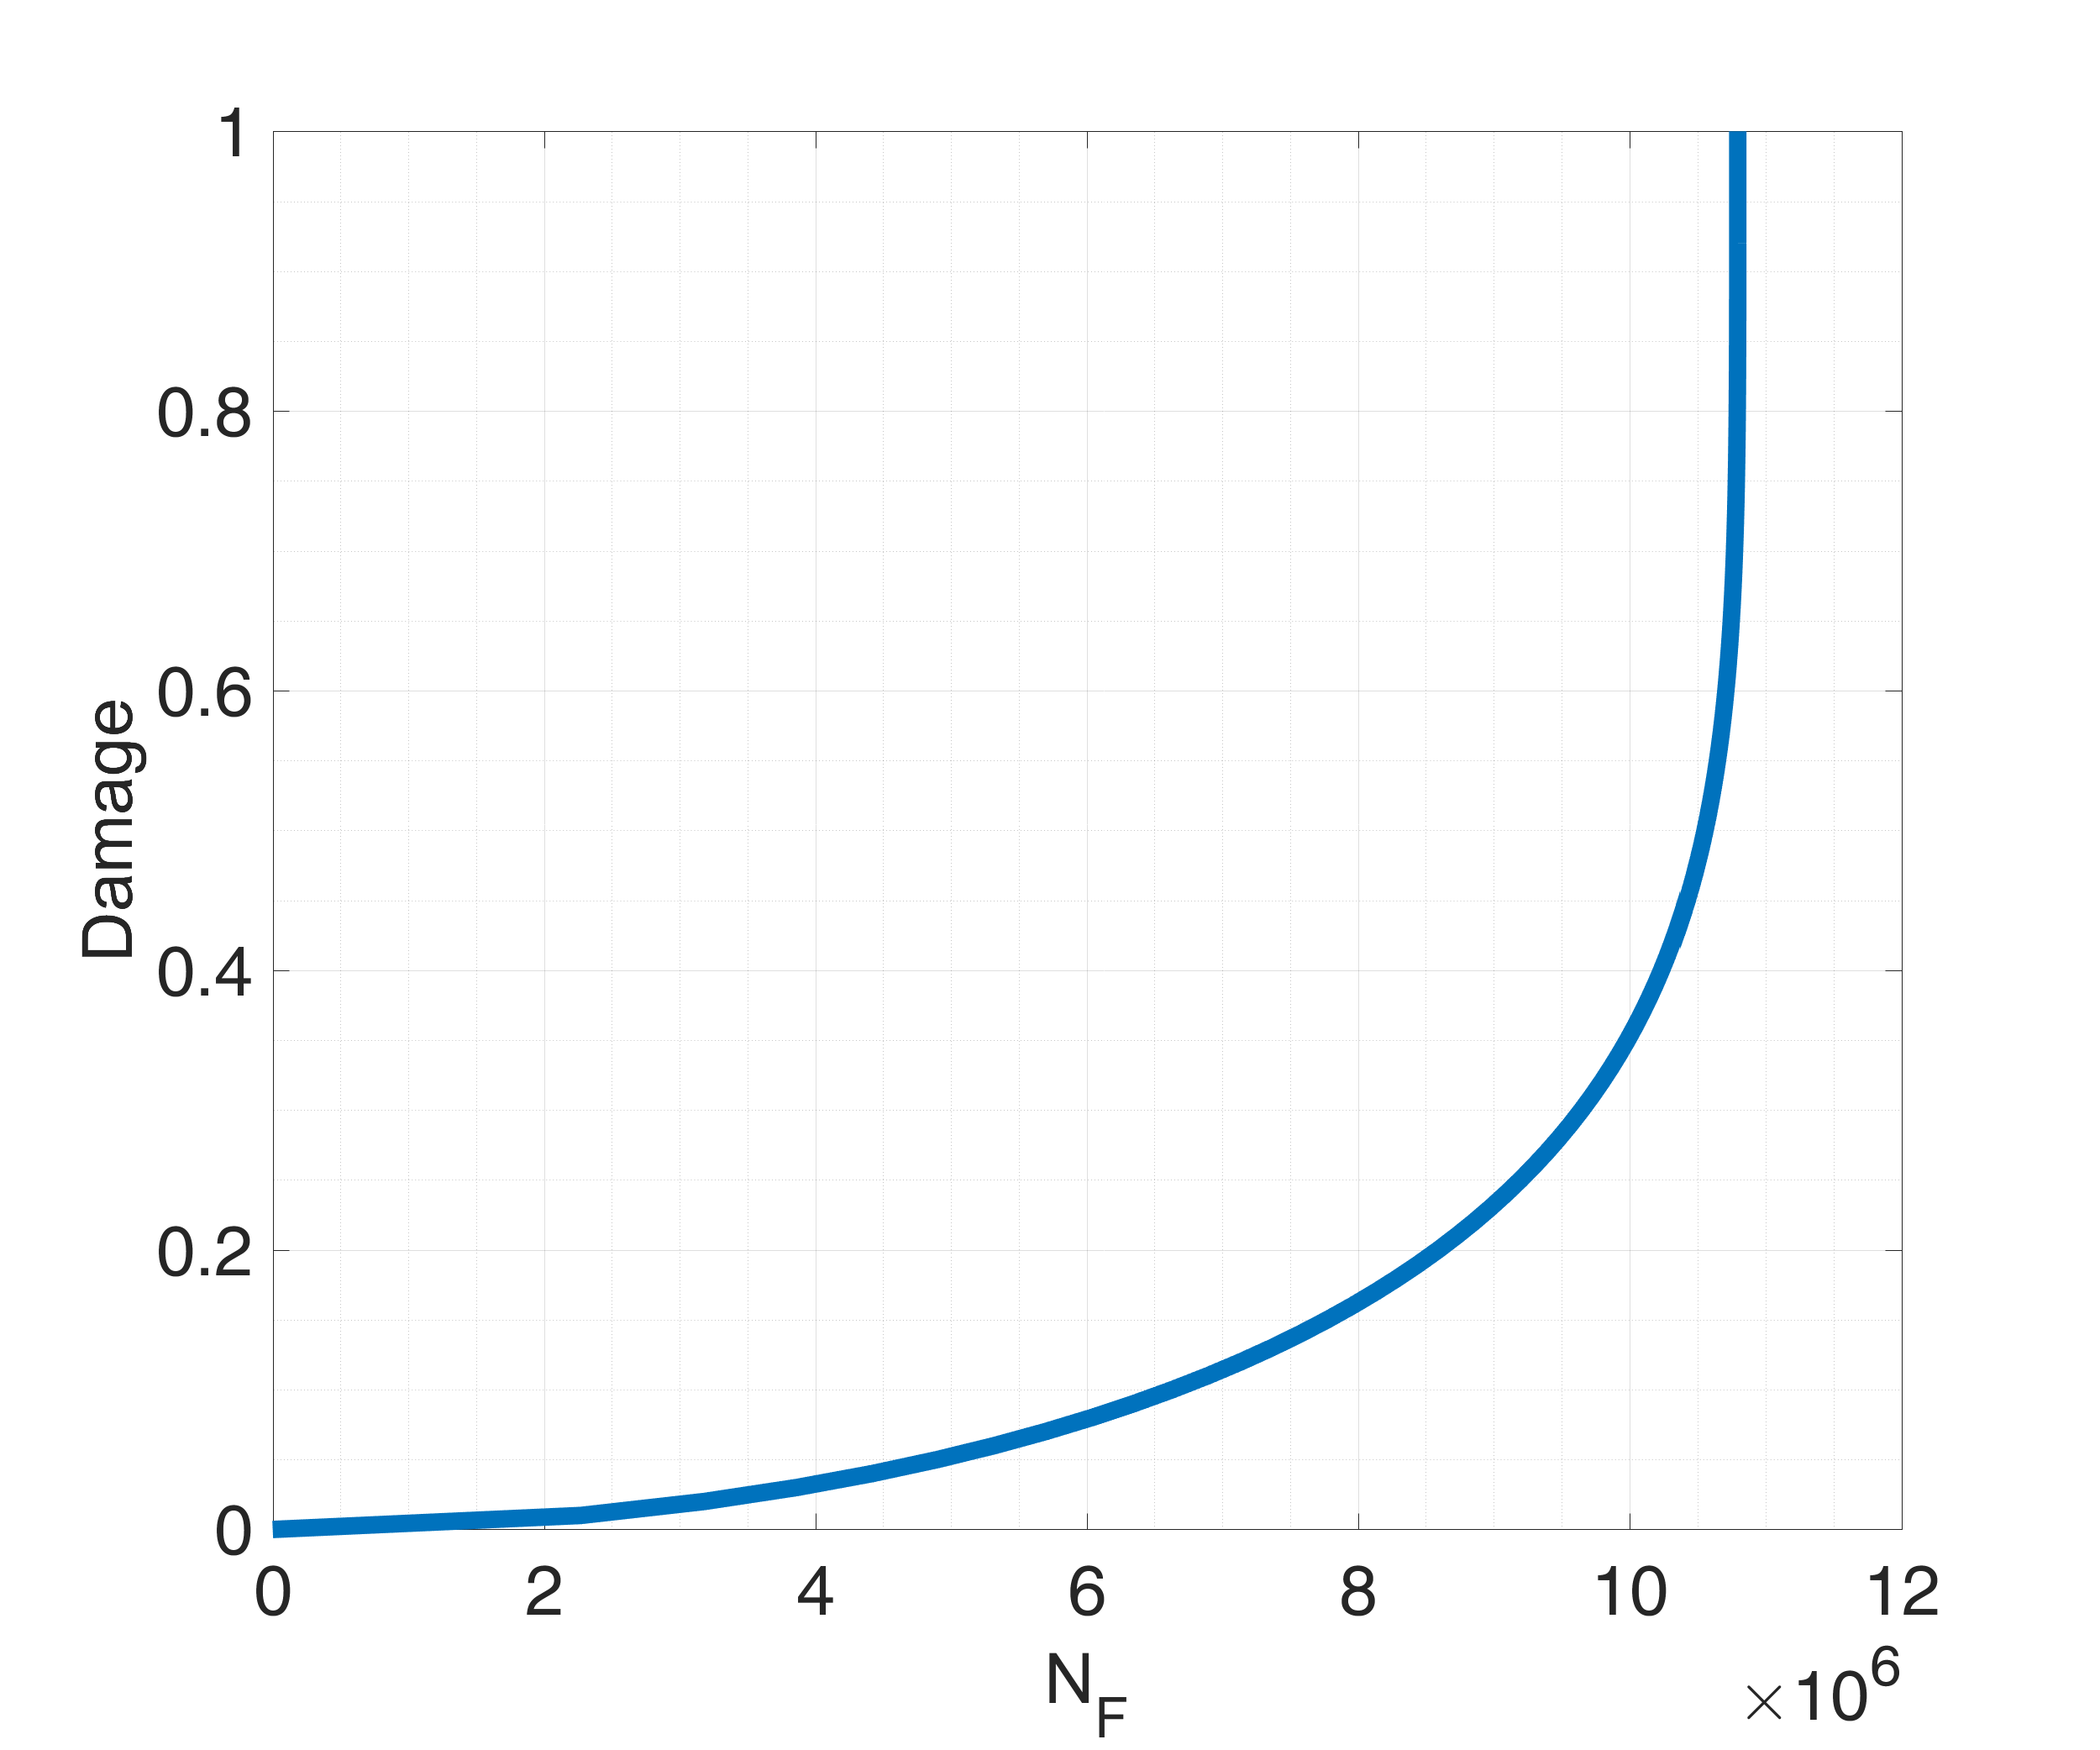
\includegraphics[width=0.8\textwidth]{figures//D-N.png} 
	\caption{Damage accumulation in terms of N in constant loading condition, with D and N are related by the evolution equation \eqref{D-N}}
	\label{DN}
\end{figure}

The number of cycles to failure, obtained at $D=1$, is: 
\begin{equation}N_F = \frac{1}{(\gamma+1)(1-\alpha)}\left[\frac{A_{\uppercase\expandafter{\romannumeral2}}}{M(\sigma_H)}\right]^{-\gamma}
\label{chaboche}
\end{equation} 

In Eq.\eqref{chaboche}, $\gamma$, $b$ and $a$ are material parameters determined from fatigue tests.

In the case of multiaxial fatigue loading, an infinite life is obtained if the stress amplitude $A_{\uppercase\expandafter{\romannumeral2}}$ respects:

\begin{equation}A_{\uppercase\expandafter{\romannumeral2}}\leqslant A_{\uppercase\expandafter{\romannumeral2}}^\ast(\sigma_H)=s_{-1}(1-3b\sigma_H).\end{equation}

In terms of Sines criterion which Chaboche uses, it writes:
\begin{equation}\sqrt{J_2}_a+3bs_{-1}\sigma_H-s_{-1}\leqslant 0.
\label{sines}
\end{equation}

Finally, $\sigma_H$ is the mean hydrostatic stress defined by:
\begin{equation}\sigma_H=\frac{1}{6}[\max tr(\uline{\uline{\sigma}}(n))+\min tr(\uline{\uline{\sigma}}(n))],\end{equation}


The damage is expressed the same as in uniaxial case:
\begin{equation}D=1-\left[ 1-\left( \frac{N}{N_F}\right) ^{\frac{1}{1-\alpha}}\right] ^{\frac{1}{\gamma+1}}.
\label{damage}
\end{equation}

\begin{figure}[h!]
	\centering
	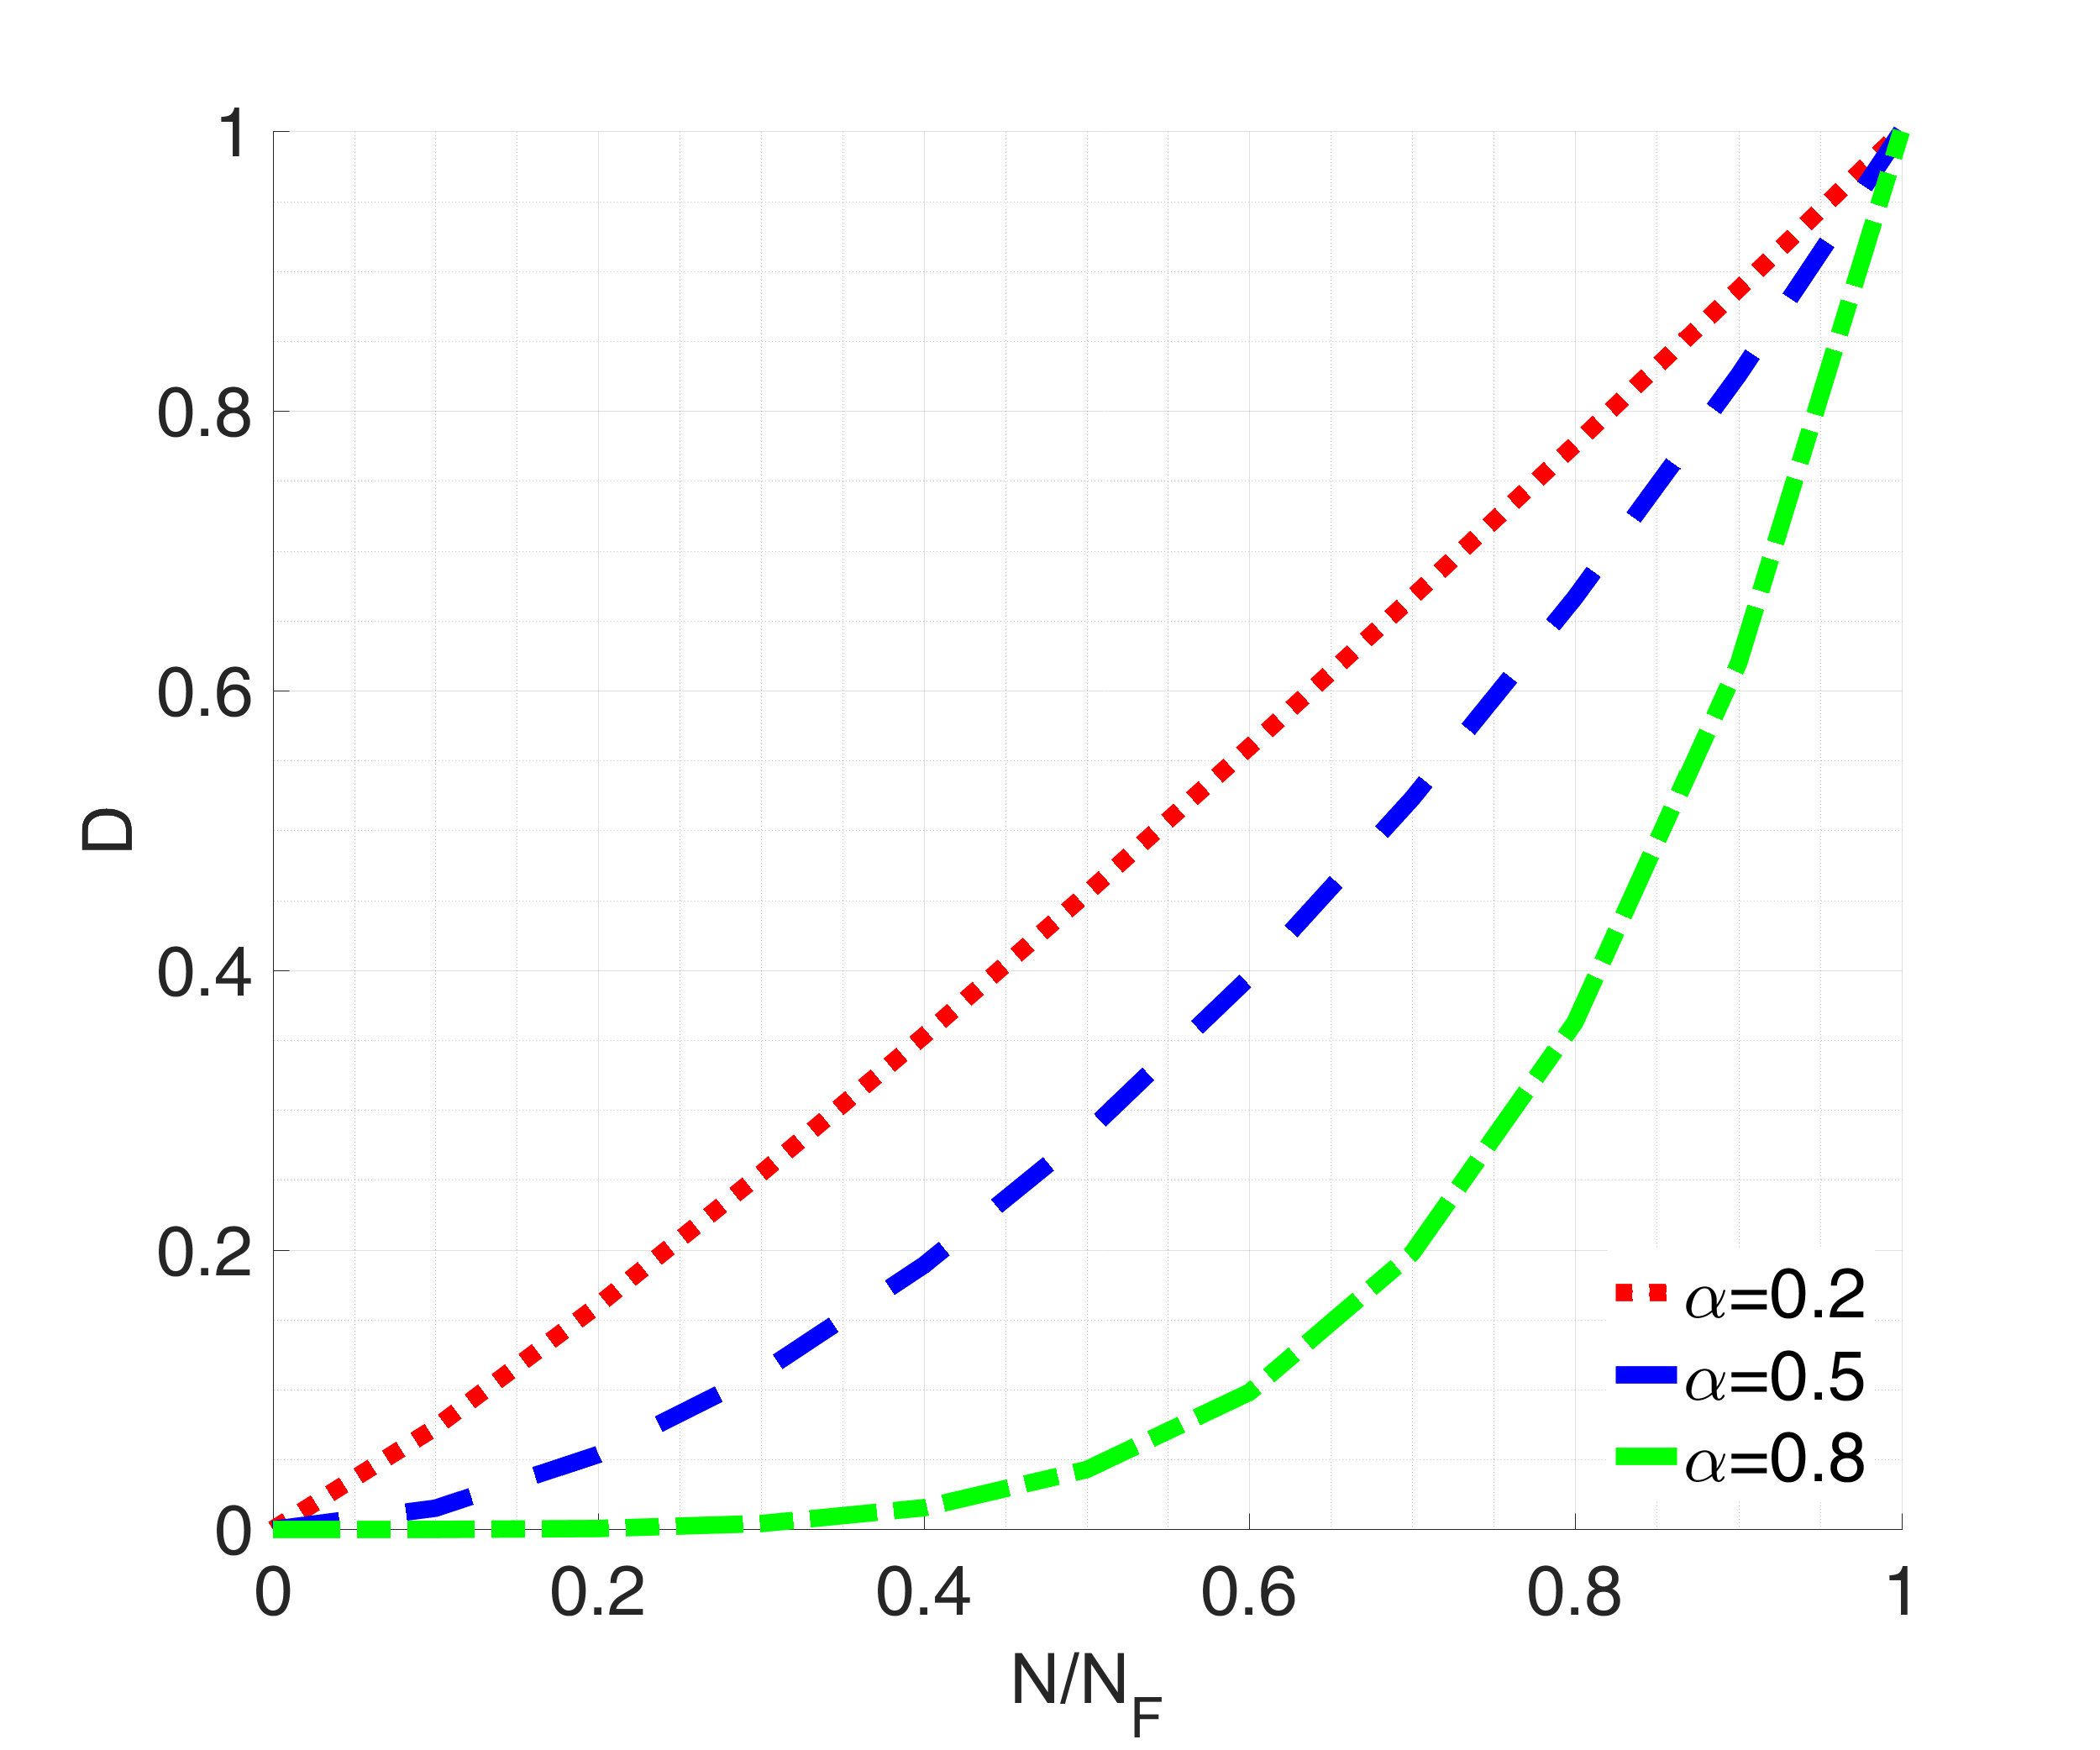
\includegraphics[width=\textwidth]{figures//Dratio1.png}
	\vspace{-12pt}
	\caption{Influence of function $\alpha$ in fatigue damage versus fatigue life ratio ($\gamma=0.1$)}
	\label{Alpha}
\end{figure}
These theories account for the nonlinear nature of fatigue damage accumulation by using nonlinear relations such as Eq.\eqref{damage} where the power $\alpha$ depends on the load level(see \figref{Alpha}).


\begin{figure}[h!]
	\centering
	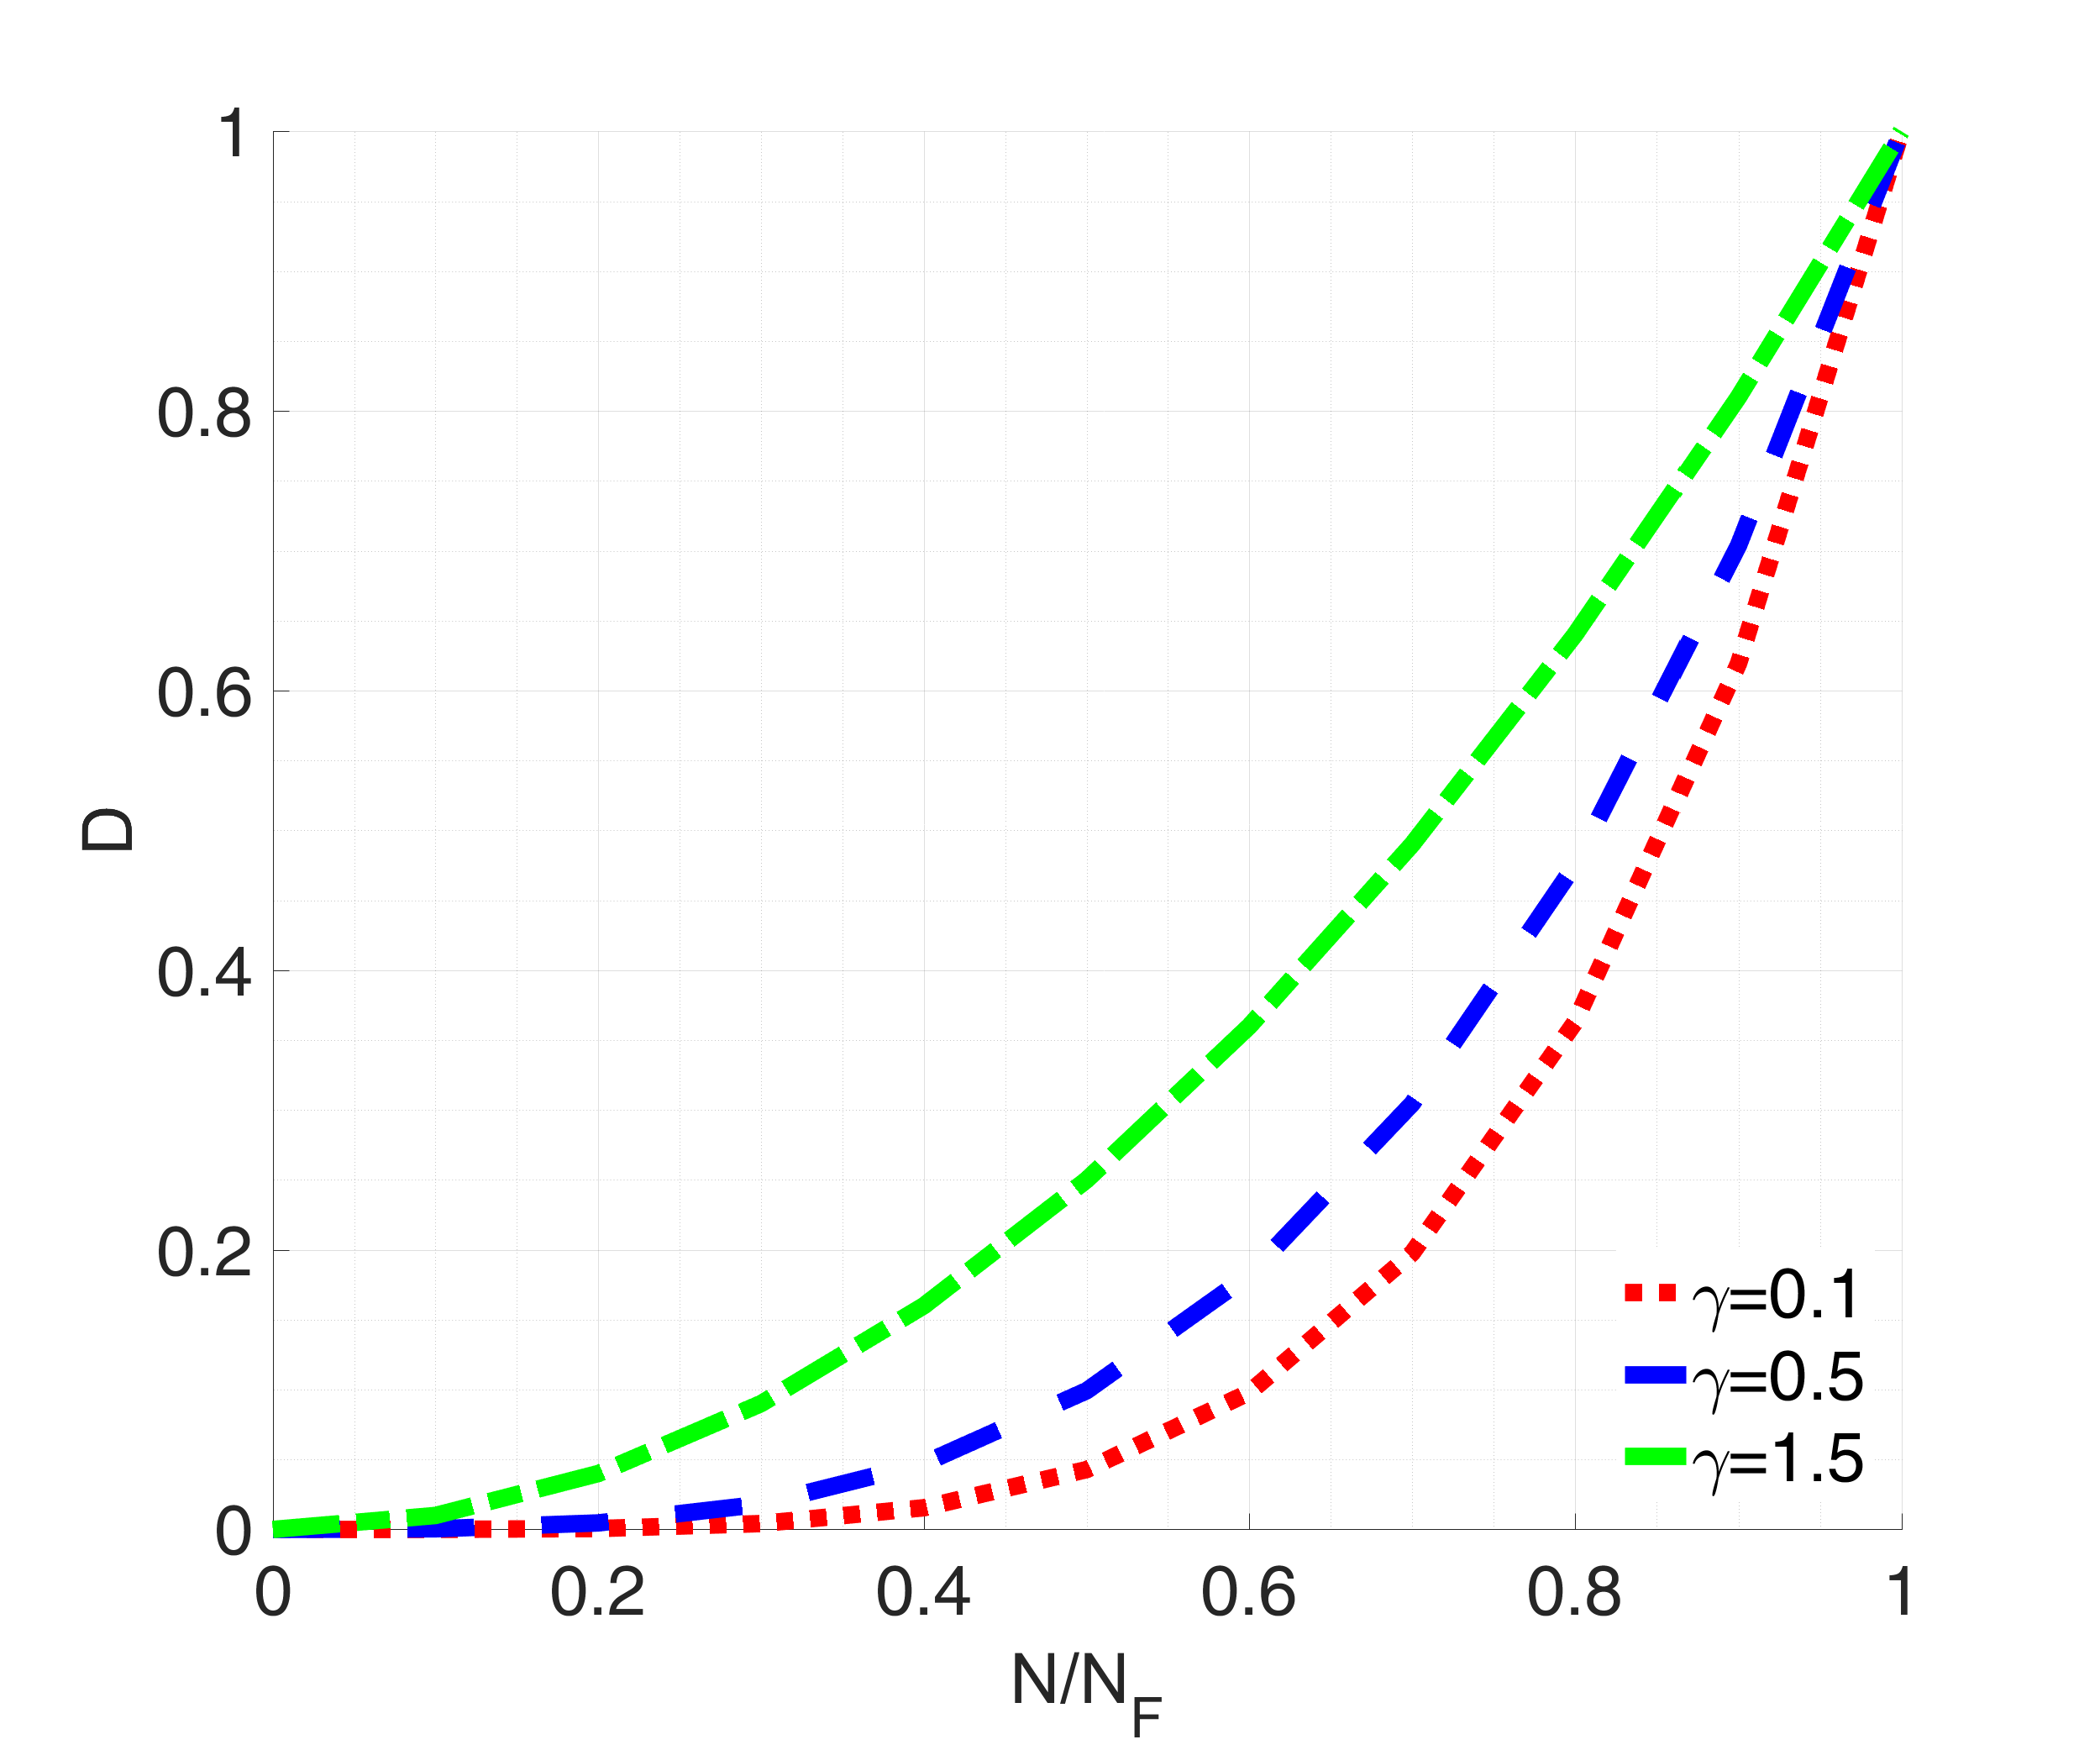
\includegraphics[width=\textwidth]{figures//Dratio2.png}
	\vspace{-12pt}
	\caption{Influence of function $\gamma$ in a plot of  damage versus fatigue life ratio with $\alpha=0.8$}
\end{figure}

\clearpage
\section{Verification method of Chaboche law}

To facilitate our verification of the law we use two-stress level loading, the specimen is firstly loaded at stress $\sigma_1$ for $N_1$ cycles and then at stress $\sigma_2$ for $N_2$ cycles until failure. We can then observe if the experimental results are satisfactory.\\
After $N_1$ cycles, we have from Eq.\eqref{damage}, a damage $D_1$ given by:
\begin{equation}
[1-(1-D_1)^{\gamma+1}]^{1-\alpha_1}=\frac{N_1}{N_{F1}}
\label{eq.23a}
\end{equation}
By integrating Eq.\eqref{diffform} from $D=D_1$ to $D=1$, we get:
\begin{equation}
1-[1-(1-D_1)^{\gamma+1}]^{1-\alpha_2}=\frac{N_2}{N_{F2}},
\end{equation}
which yields:
\begin{equation}1-\frac{N_2}{N_{F2}}=1-[1-(1-D_1)^{\gamma+1}]^{1-\alpha_2}.
\label{eq.23b}
\end{equation}
From Eq.\eqref{eq.23a} and Eq.\eqref{eq.23b}, after elimination of $[1-(1-D_1)^{\gamma+1}]$ we get:
\begin{equation} \frac{N_2}{N_{F2}}=1-(\frac{N_1}{N_{F1}})^\frac{1-\alpha_2}{1-\alpha_1}=1-(\frac{N_1}{N_{F1}})^\eta\end{equation}
with
\begin{equation}
		\begin{split}
			\eta&=\frac{1-\alpha_2}{1-\alpha_1}
			\\&=\frac{A_{\uppercase\expandafter{\romannumeral2 2}} - A_{\uppercase\expandafter{\romannumeral2}}^\ast(P_{m2})}{A_{\uppercase\expandafter{\romannumeral2 1}} - A_{\uppercase\expandafter{\romannumeral2}}^\ast(P_{m1})}\frac{ \sigma_{u} - \sigma_{eqMax1}}{ \sigma_{u} - \sigma_{eqMax2}}
			\\&=\frac{\sqrt{J_{2,a_2}} - s_{-1}(1-3bP_{m_2})}{\sqrt{J_{2,a_1}} - s_{-1}(1-3bP_{m_1})}\frac{ \sigma_{u} - \max(2\sqrt{J_{2,a_1}})}{  \sigma_{u} - \max(2\sqrt{J_{2,a_2}})}
	\end{split}
\label{eq.etachaboche}
\end{equation}

In the case of high-low loading sequence($\sigma_1>\sigma_2 \; or \; \alpha_1<\alpha_2$):

$$\eta=\frac{1-\alpha_2}{1-\alpha_1}<1\Rightarrow \frac{N_2}{N_{F2}}=1-(\frac{N_1}{N_{F1}})^\eta<1-\frac{N_1}{N_{F1}},$$

in other words, we have 
$$\frac{N_1}{N_{F1}}+\frac{N_2}{N_{F2}}<1.$$

The cumulative damage under high-low loading sequence, as we deduced, has the addition of partial lives less than 1. 

Similarly, the cumulative damage under low-high loading sequence has has a beneficial effect: 
$$\frac{N_1}{N_{F1}}+\frac{N_2}{N_{F2}}>1.$$

For constant two-level stress loading, $\alpha_1=\alpha_2$, the Chaboche law returns to the miner's rule where we have:
$$\frac{N_1}{N_{F1}}+\frac{N_2}{N_{F2}}=1.$$
\section{Chaboche law containing different criteria}
\subsection{Chaboche law with Crossland criterion}

In the previous model we used Sines fatigue criterion constructing the damage criterion exponent $\alpha$. Now we want to test Chaboche law with different criteria and compare the numerical results. Since $\alpha$ represents the internal variables and contains the fatigue criterion, we first change $\alpha$ to satisfy Crossland Criterion:

\begin{equation}\alpha = 1 - a\left\langle \frac{\max\limits_{n}\sqrt{J_2}_a(n)+a_c{P_{max}(n)}-b_c}{ \sigma_{u} - 2\max\sqrt{J_2}_a}\right\rangle,\end{equation}

with
\begin{equation}
a_c=\frac{(t_{-1}-\frac{f_{-1}}{\sqrt{3}})}{\frac{f_{-1}}{3}}, \quad 
b_c=t_{-1}.
\end{equation}

Therefore, the coefficient $\eta$ characterizing the high low sequential loading will now be given by
\begin{equation}\eta_c=\frac{1-\alpha_2}{1-\alpha_1}=
\frac{\sqrt{J_{2,a_2}}+a_cP_{M_2}-b_c}{\sqrt{J_{2,a_1}}+a_cP_{M_1}-b_c}\frac{ \sigma_{u} - \max(2\sqrt{J_{2,a_1}})}{  \sigma_{u} - \max(2\sqrt{J_{2,a_2}})}.
\end{equation}

In Eq.\eqref{chabochemulti} and \eqref{D-N}, the amplitude of octahedral shear stress $A_{\uppercase\expandafter{\romannumeral2}}$ remain unchanged.

\subsection{Chaboche law with Dang Van criterion}

We can also change $\alpha$ to express it through Dang Van Criterion, leading to:

\begin{equation}\alpha = 1 - a\left\langle \frac{\max\limits_{n}\left\{\tau{(n)}+a_DP{(n)}\right\}-b_D}{ \sigma_{u} - 2\max\sqrt{J_2}_a}\right\rangle.\end{equation}

with
\begin{equation}
\tau(n)=\frac{1}{2}(\hat{\sigma}_{\Rmnum{1}}(n)-\hat{\sigma}_{\Rmnum{3}}(n))
\end{equation}
$$a_D=\frac{3t_{-1}}{f_{-1}}-\frac{3}{2}, b_D=t_{-1}.$$
In this case, the coefficient $\eta$ of high low sequential loading becomes
\begin{equation}\eta_D=\frac{1-\alpha_2}{1-\alpha_1}=
\frac{\max\limits_{t}\left\{\tau_2{(n)}+a_DP_2{(n)}\right\}-b_D}{\max\limits_{t}\left\{\tau_1{(n)}+a_DP_1{(n)}\right\}-b_D}\frac{ \sigma_{u} - \max(2\sqrt{J_{2a_1}})}{  \sigma_{u} - \max(2\sqrt{J_{2a_2}})}
\end{equation}
In Eq.\eqref{chabochemulti} and \eqref{D-N}, we change $A_{\uppercase\expandafter{\romannumeral2}}$ to $\max\tau(n)$:
\begin{equation}N_F = \frac{1}{(\gamma+1)(1-\alpha)}\left[\frac{\max\tau(n)}{M(\sigma_H)}\right]^{-\gamma}
\label{dvchaboche}
\end{equation} 

\section{Numerical testing on different loading patterns}
The fatigue limit with different criteria are distinctive. We compare different criteria in a $A_{\uppercase\expandafter{\romannumeral2}}-N_F$ figure as predicted in Eq.\eqref{chaboche}. Here
$\gamma$, $b$ and $a$ are material parameters determined from fatigue tests.

In this case we have 
$$N_F = \frac{1}{(\gamma+1)(1-\alpha)}\left[\frac{A_{\uppercase\expandafter{\romannumeral2}}}{M(\sigma_H)}\right]^{-\gamma},$$

$$M(\sigma_H)=s_{-1}\left(1-3\sigma_H/\sigma_u\right).$$

For Sines and Crossland criteria:

$$A_{\uppercase\expandafter{\romannumeral2}}=\sqrt{J_2}_a=\frac{1}{2}\max\limits_{t}\sqrt{\frac{1}{2}(\Delta s_{11}^2+\Delta s_{22}^2+\Delta s_{33}^2+2\Delta s_{12}^2+2\Delta s_{13}^2+2\Delta s_{23}^2)}.$$

For Dang Van criterion:
$$A_{\uppercase\expandafter{\romannumeral2}}= \max\tau(n).$$ 

\newpage
\subsection{Test on pure rotation}

From the fatigue zone we select $r=0.1$ as the radius to study. We select here:

$s_{-1}=f_{-1}=0.8MPa$,

$\sigma_{u}=1.67MPa$ 

$\gamma=6$


$A_{\uppercase\expandafter{\romannumeral2}}-N_F$ figure is shown in \figref{JNrotation}. 
\begin{figure}[h!]
	\centering
	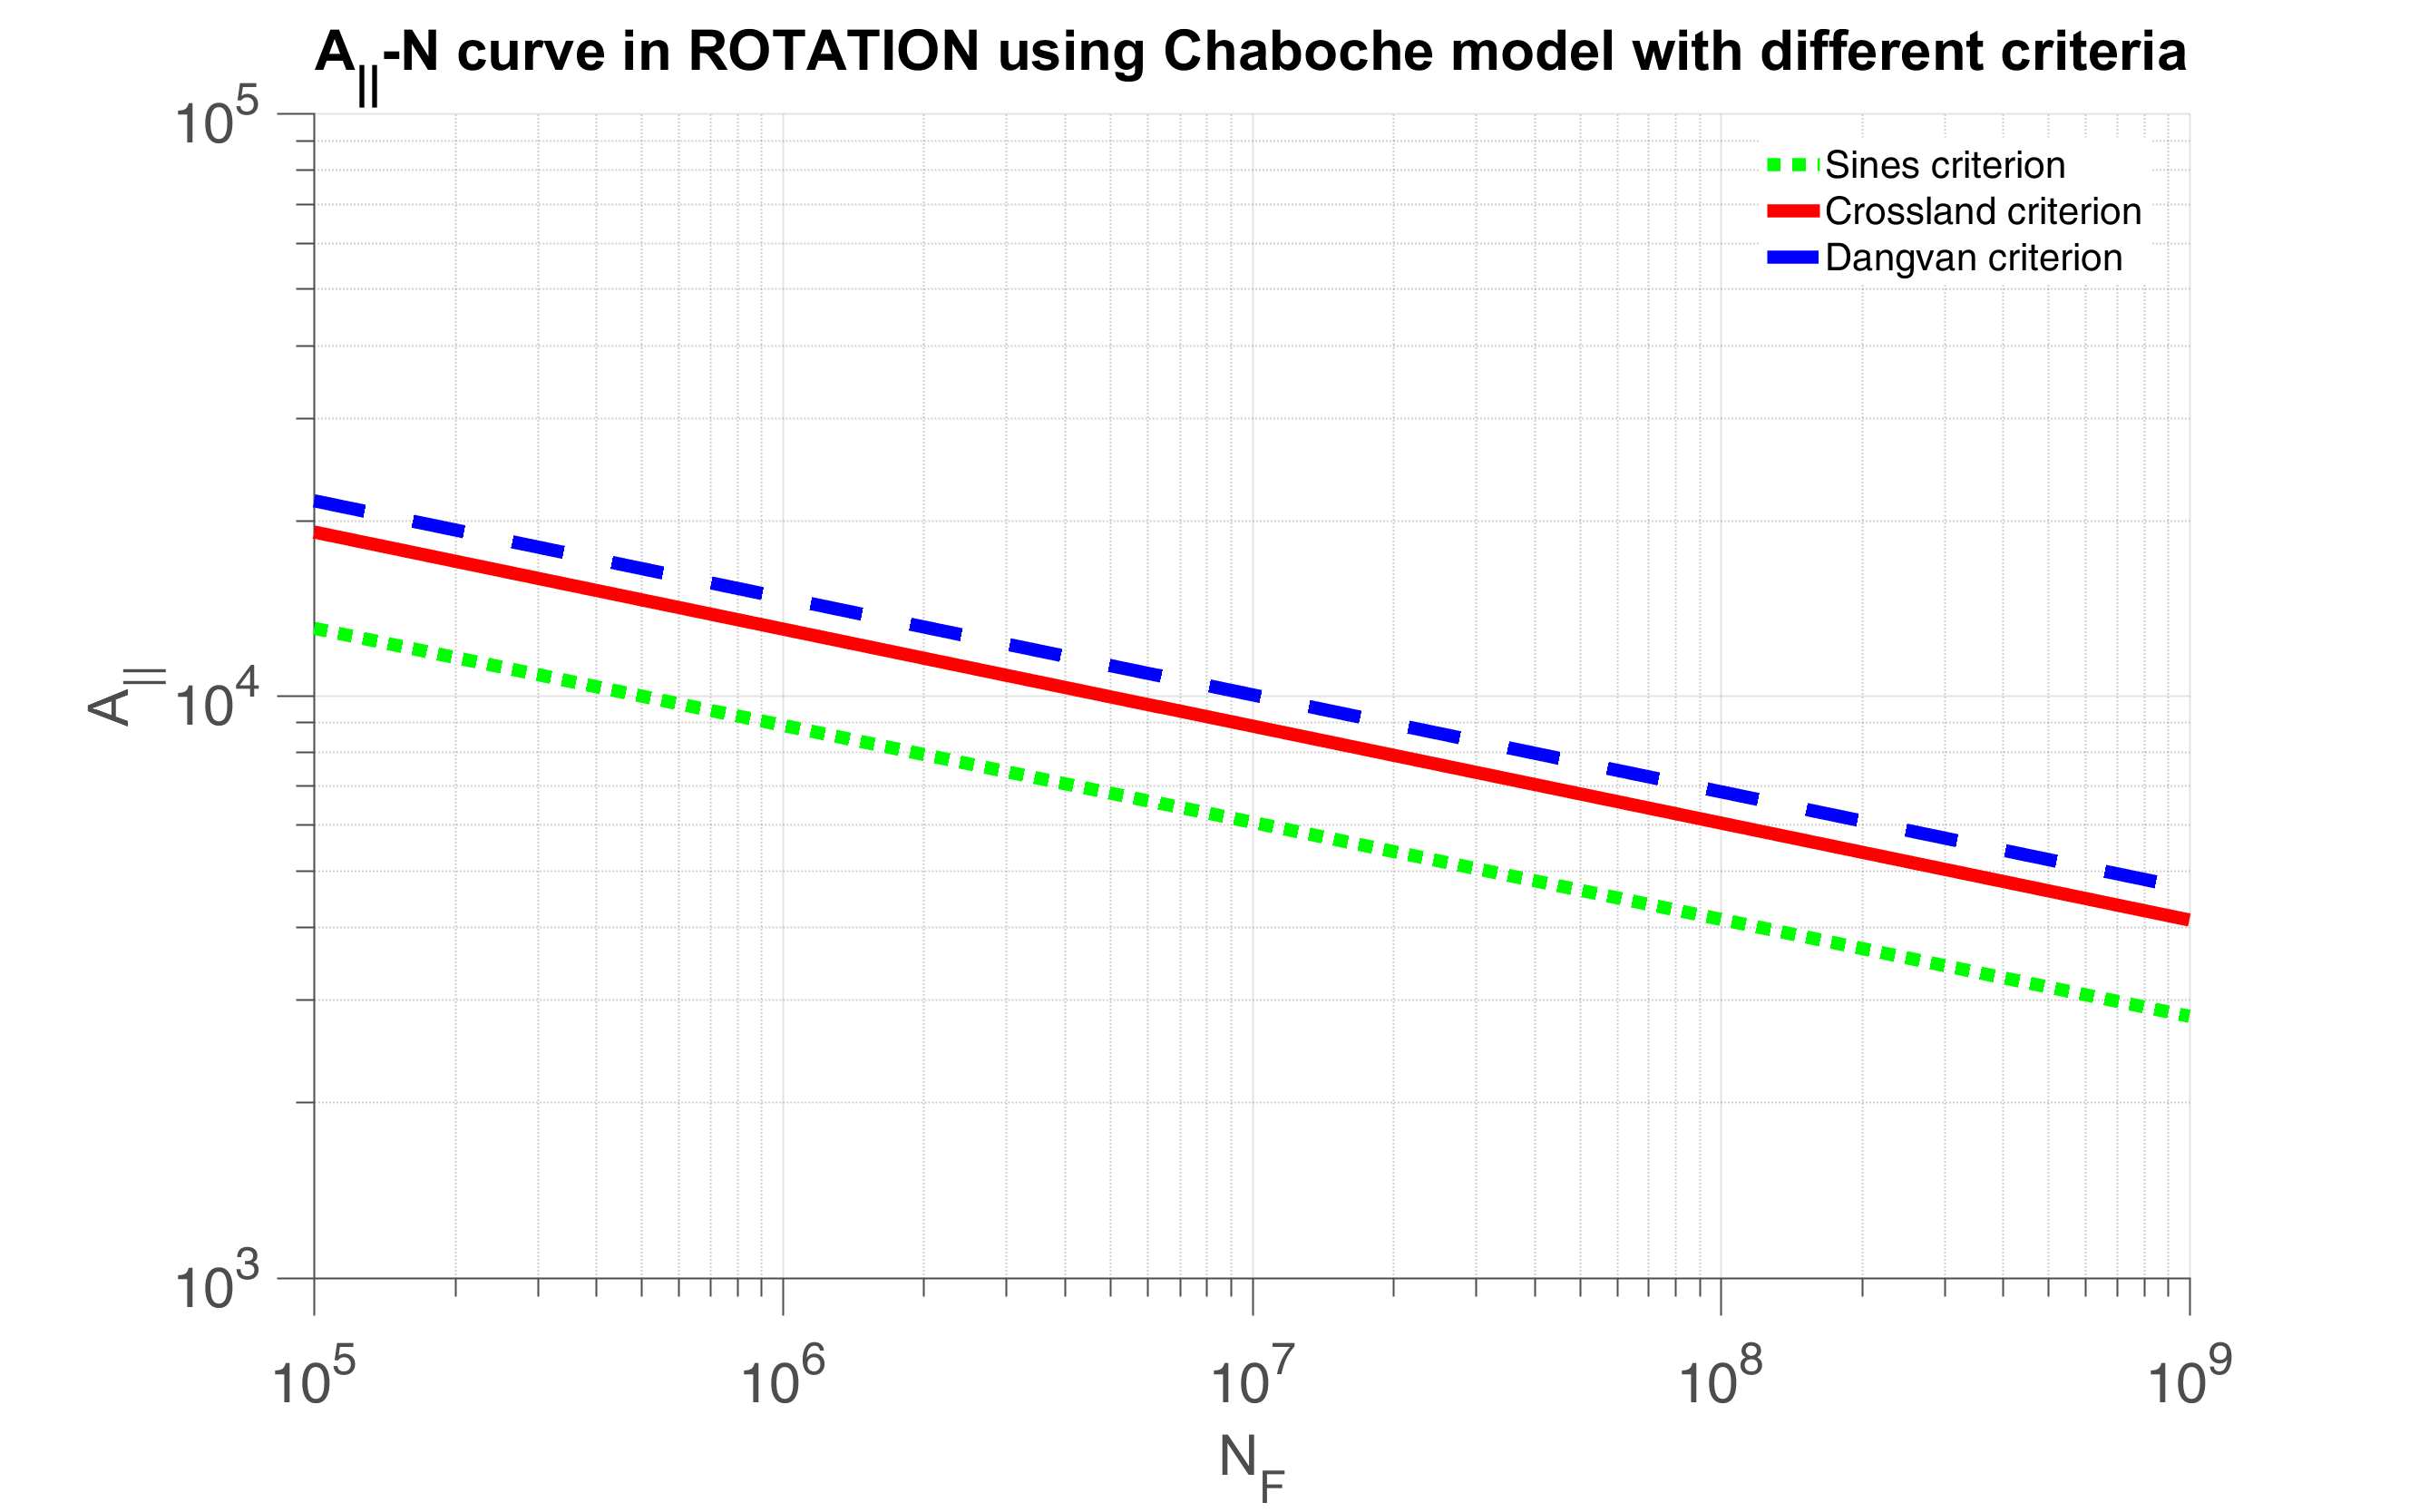
\includegraphics[width=\textwidth]{figures//JNrotation.png} 
	\caption{$A_{\uppercase\expandafter{\romannumeral2}}-N_F$ curve in rotation at r=0.1}
	\label{JNrotation}
\end{figure}

In pure rotation, we assume the first and second rotating speed are respectively $w_1=20rpm$ and $w_2=15rpm$.  

\vspace{6pt}
$A_{\uppercase\expandafter{\romannumeral2}1}=\sqrt{J_{2,a_1}}=7.7606E5 Pa$

\vspace{6pt}
$A_{\uppercase\expandafter{\romannumeral2}2}=\sqrt{J_{2,a_2}}=4.3653E5 Pa$

\vspace{6pt}
$P_{m_1}=8.8342E5 Pa$

\vspace{6pt}
$P_{m_2}=4.9693E5 Pa$

Substituting the above to Eq.\eqref{eq.etachaboche}, we can get $\eta$ in High-Low sequence and in Low-High sequence as shown in Table.\ref{tab.etarotation}:

\begin{table}[!h]
	\centering
	\begin{tabular}{llll}
		\hline
		$\eta$ value   & Sines  & Crossland & Dang Van \\ \hline
		High-low & 0.0721 & 0.0219    & 0.0121   \\
		Low-high & 13.8654 & 45.6118   & 82.5689  \\ \hline
	\end{tabular}
	\caption{$\alpha$ induced sequence effect parameter $\eta$ value with different criteria in pure rotation}
	\label{tab.etarotation}
\end{table}

The predicted results are shown in \figref{2stressR}.

\begin{figure}[h!]
	\centering
	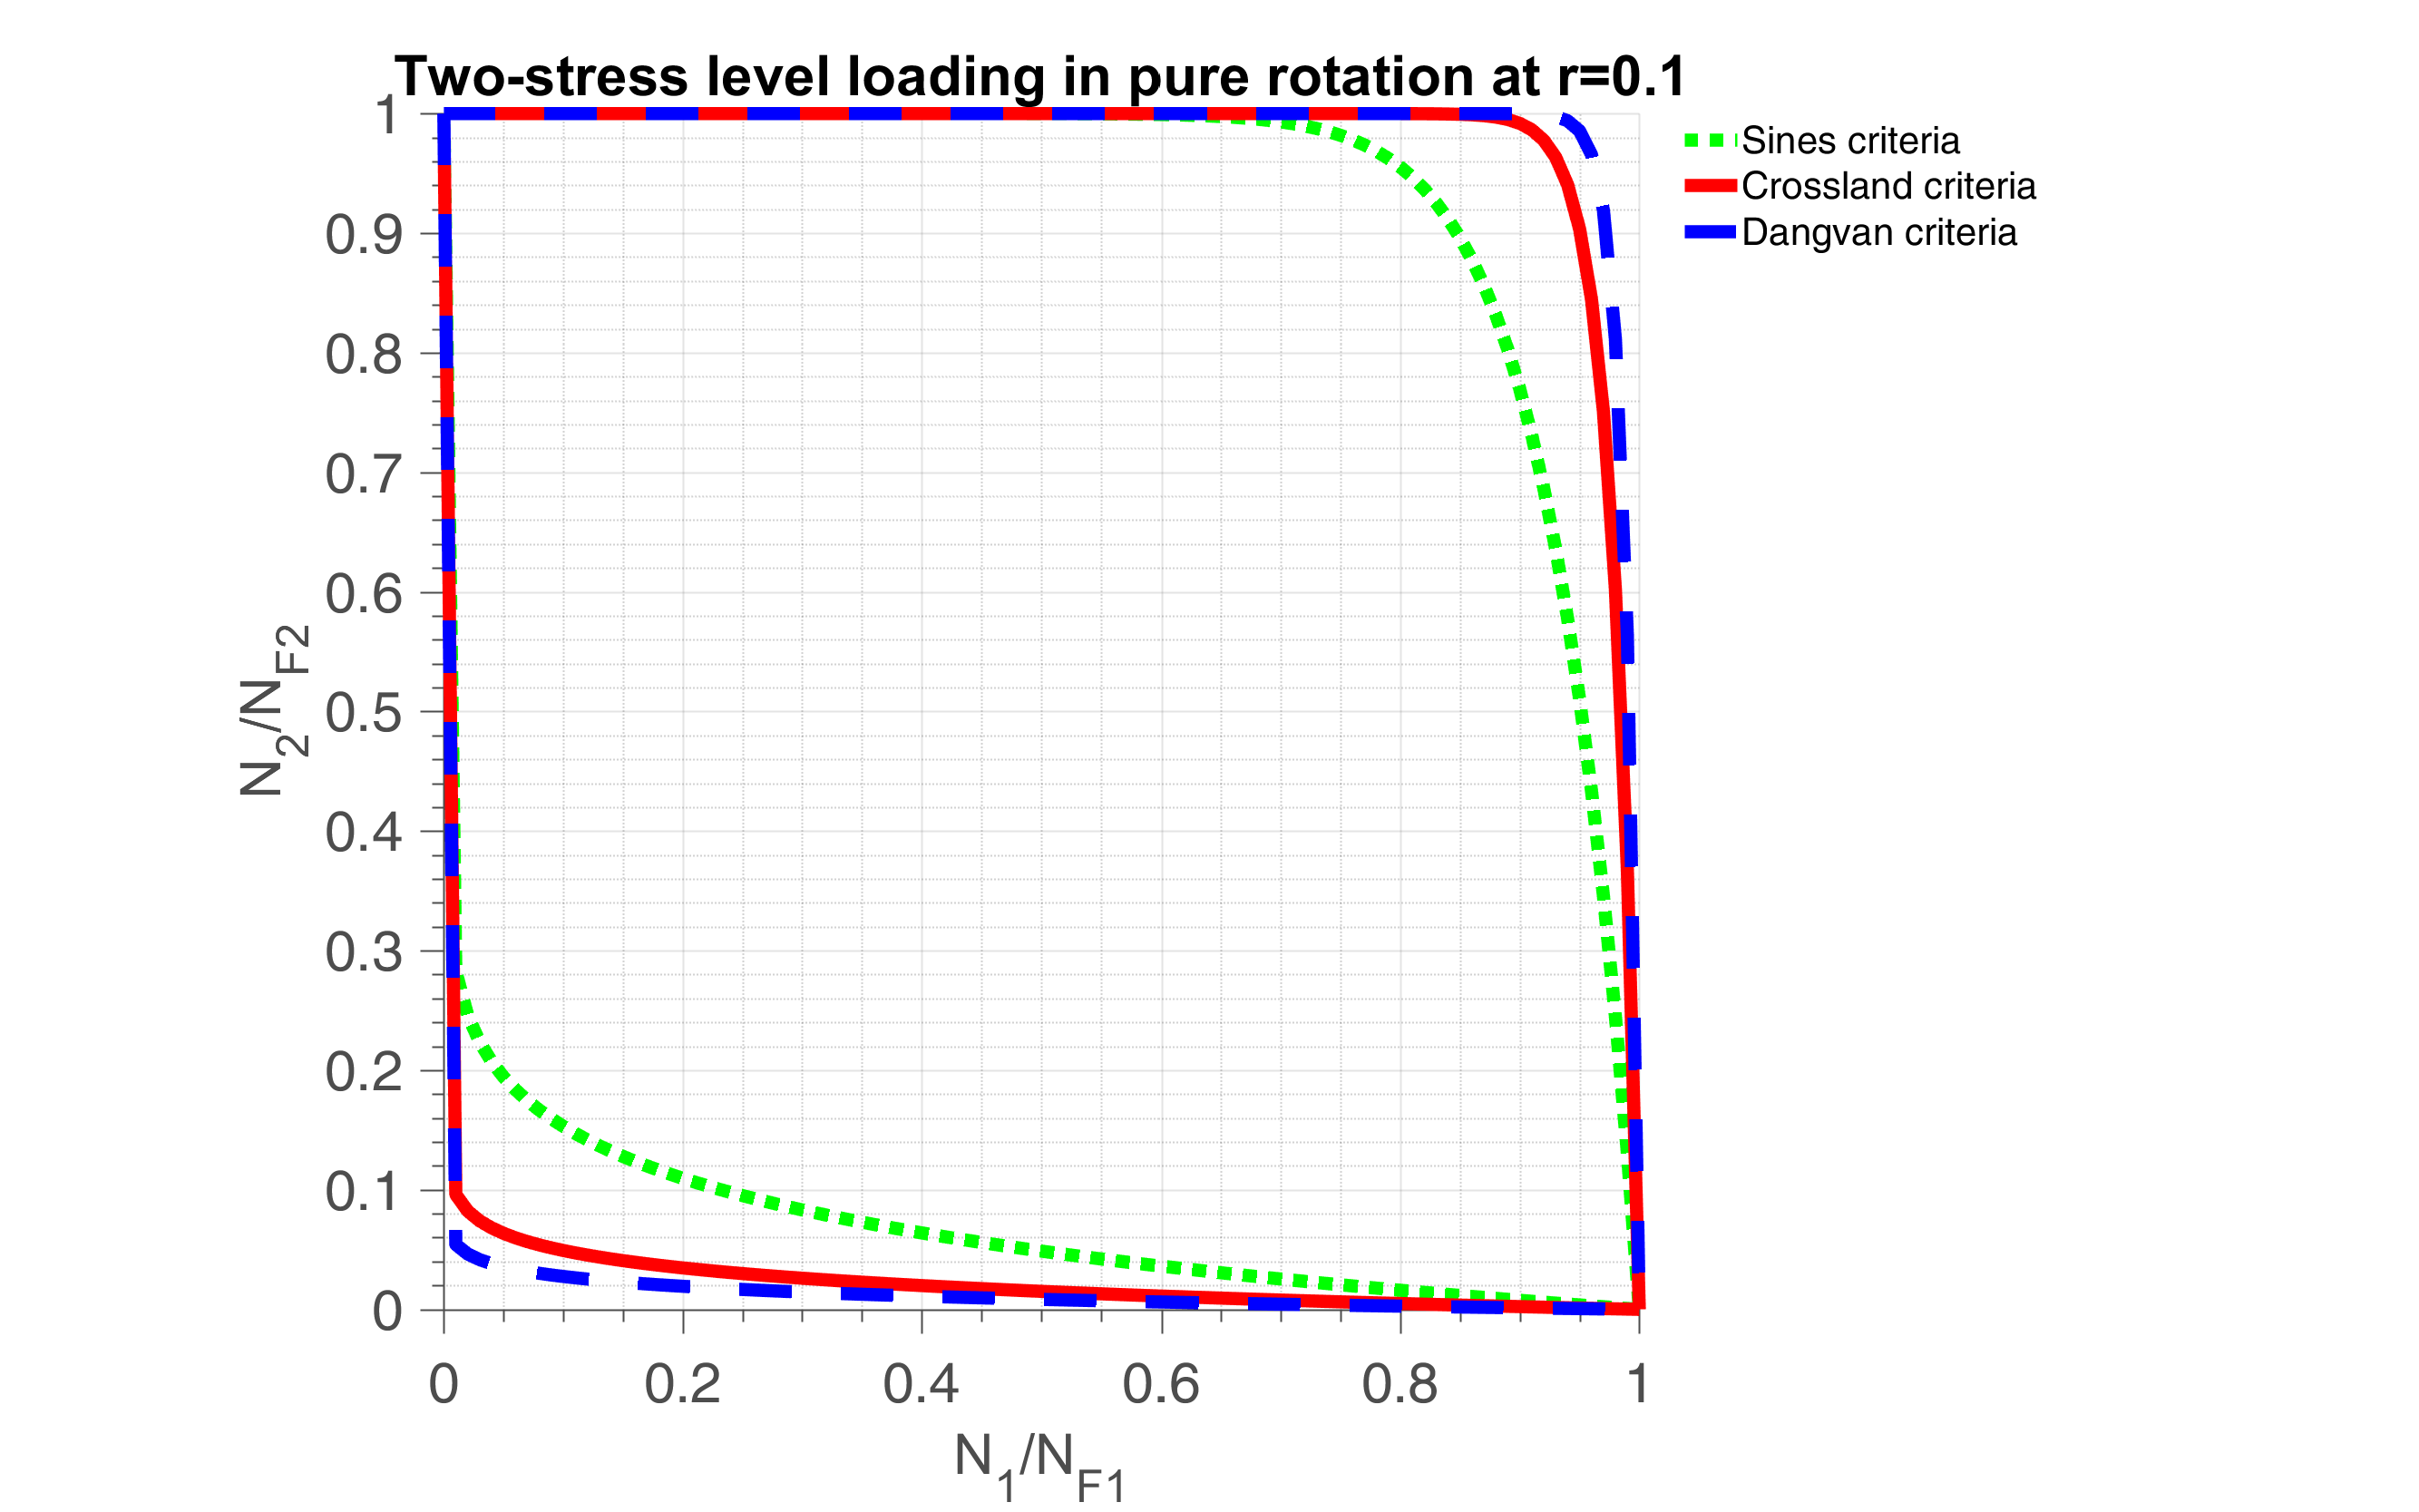
\includegraphics[width=\textwidth]{figures//2stressR.png} 
	\caption{Two-stress level loading in pure rotation at r=0.1}
	\label{2stressR}
\end{figure}

\newpage
\subsection{Test on 4-point bending}
From the fatigue zone we select $y=3$ to study. We select here:

$s_{-1}=f_{-1}=0.8MPa$,

$\sigma_{u}=1.67MPa$ 

$\gamma=6$

The $A_{\uppercase\expandafter{\romannumeral2}}-N_F$ figure is shown in \figref{JNbending}.
\begin{figure}[h!]
	\centering
	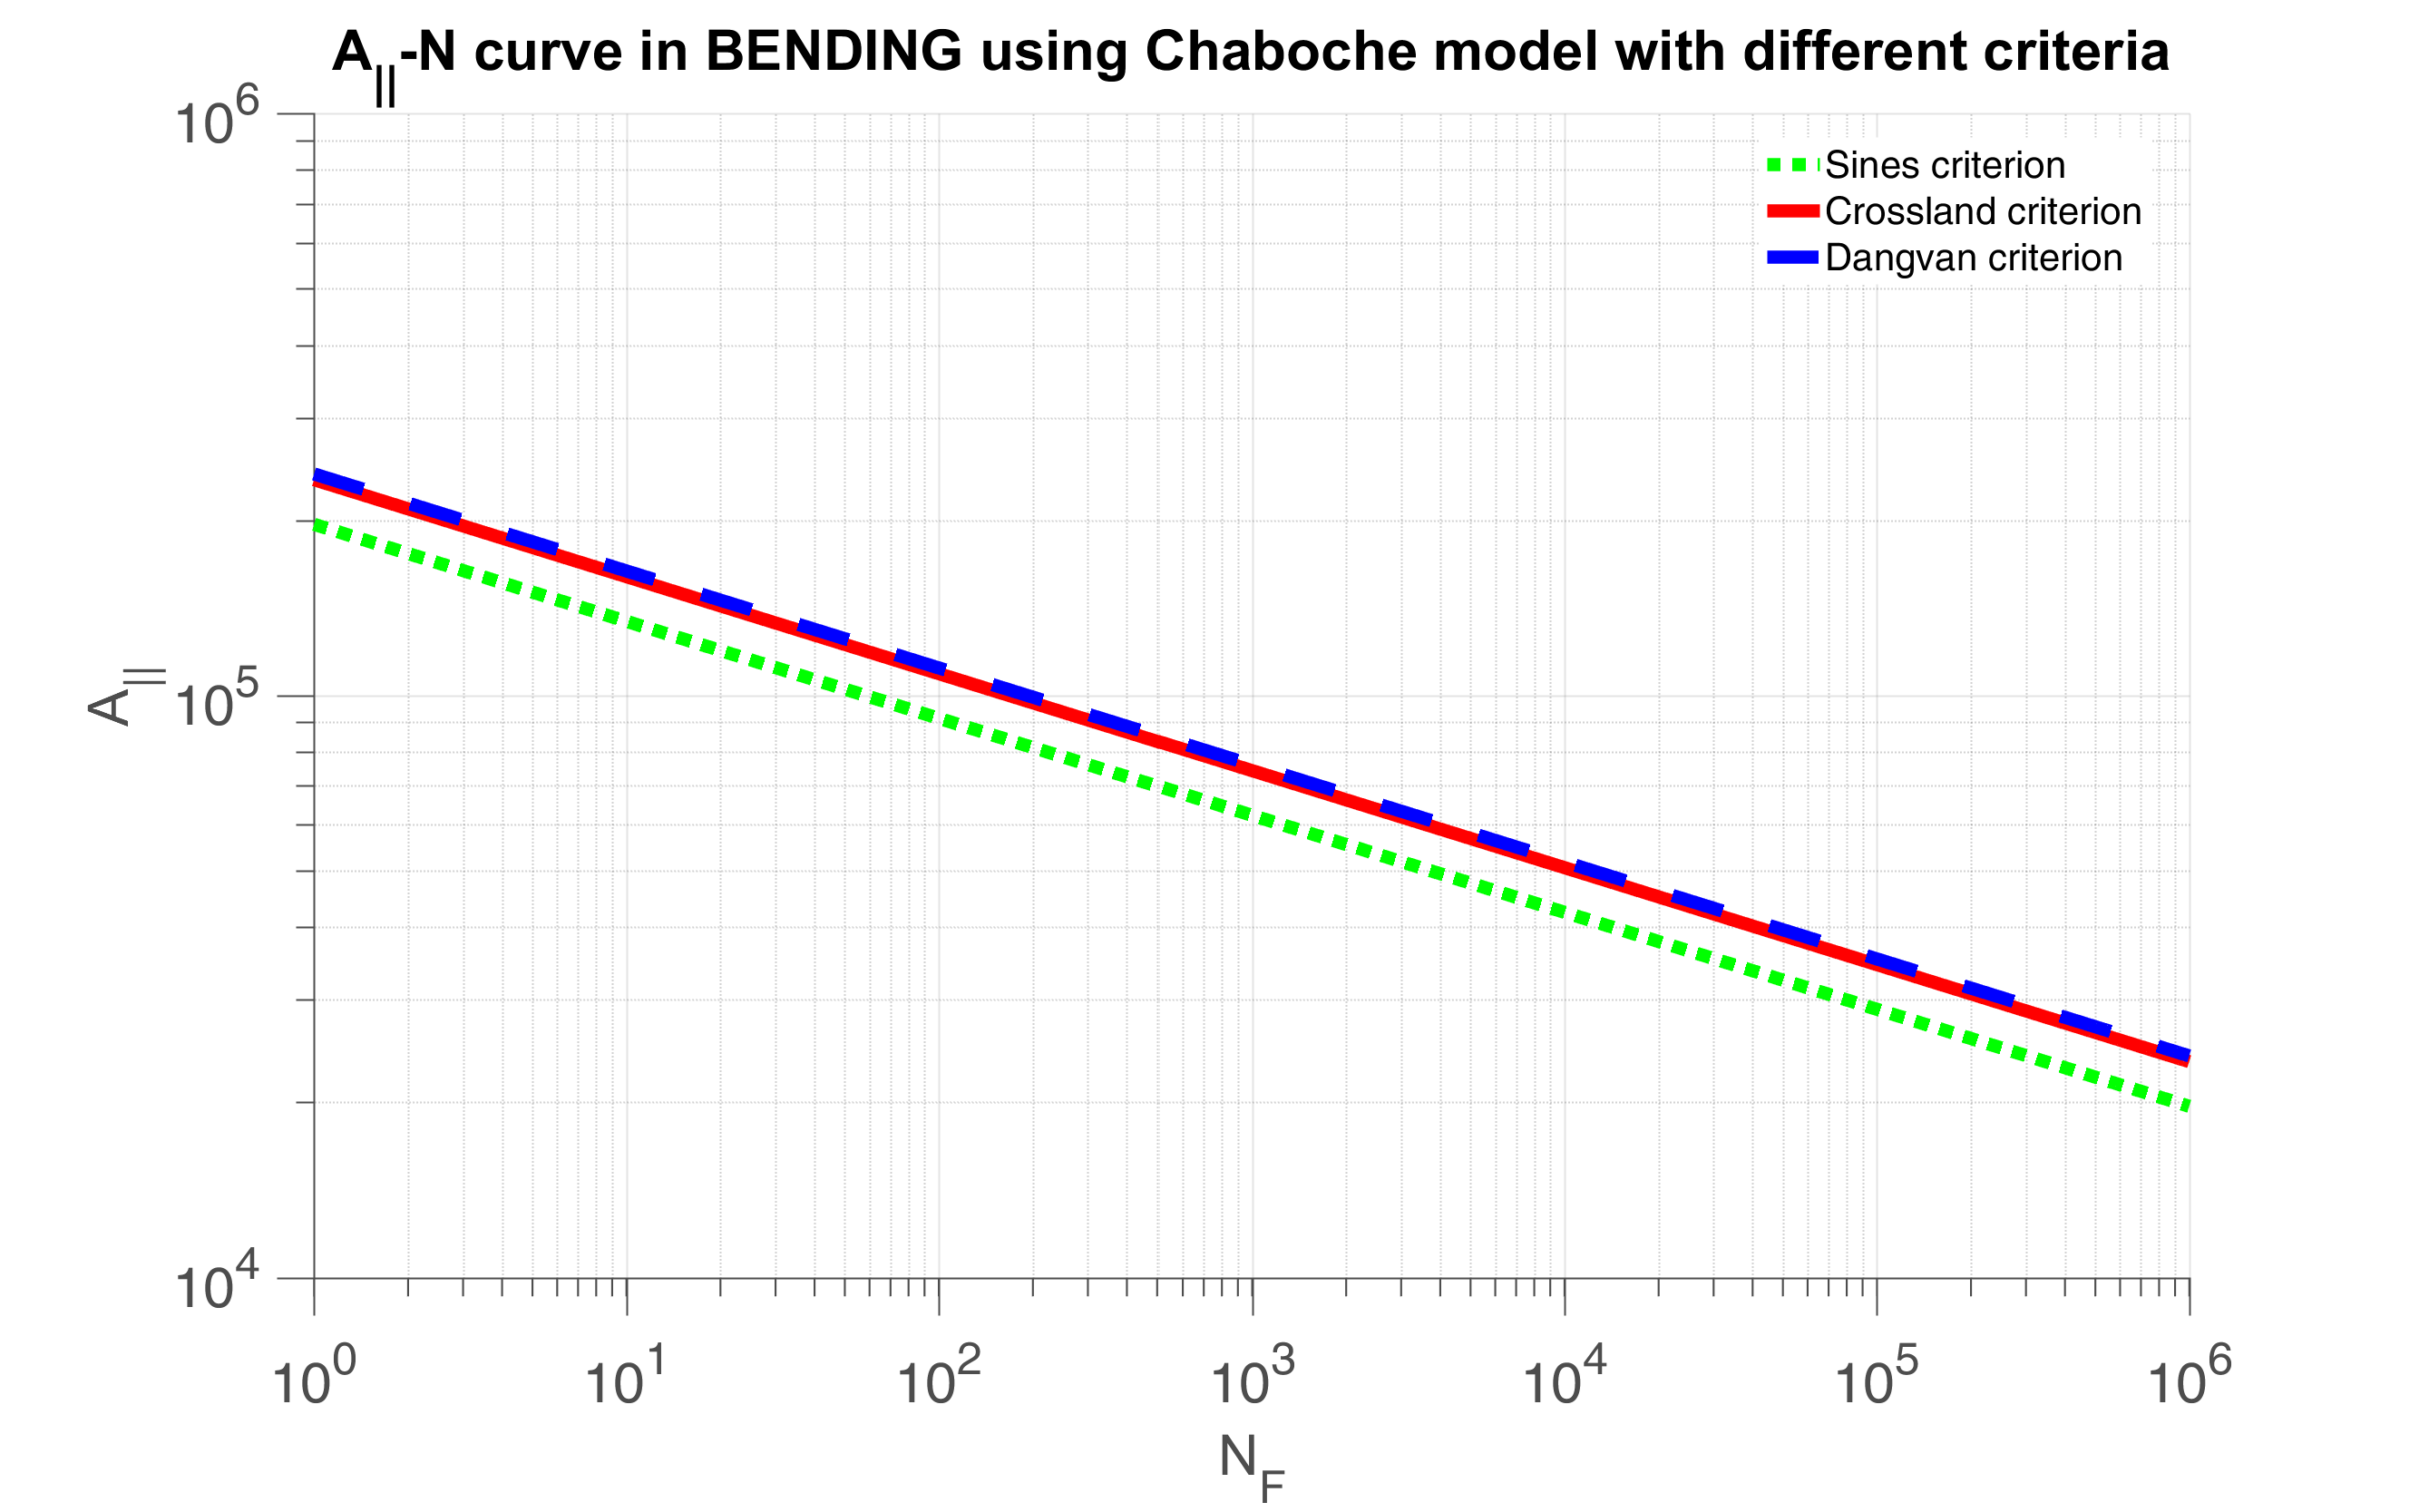
\includegraphics[width=\textwidth]{figures//JNbending.png} 
	\caption{$A_{\uppercase\expandafter{\romannumeral2}}-N_F$ curve in 4-point bending at y=3}
	\label{JNbending}
\end{figure}

In 4-point bending,we assume the first and second loading are respectively $F_1=1E6 N$ and $F_2=0.8E6 N$. 

\vspace{6pt}
$\sqrt{J_{2a_1}}=7.2194E5 Pa$

\vspace{6pt}
$\sqrt{J_{2a_2}}=5.7755E5 Pa$

\vspace{6pt}
$P_{m_1}=3.9298E5 Pa$

\vspace{6pt}
$P_{m_2}=3.1438E5 Pa$

Substituting the above to Eq.\eqref{eq.etachaboche} we can get $\eta$ in High-Low sequence:
and in Low-High sequence as shown in Table.\ref{tab.etabending}:
\begin{table}[!h]
	\centering
	\begin{tabular}{llll}
		\hline
		$\eta$ value   & Sines  & Crossland & Dang Van \\ \hline
		High-low & 0.3174 & 0.1894    &  0.1659   \\
		Low-high & 3.1510 & 5.2794   & 6.0280  \\ \hline
	\end{tabular}
	\caption{$\alpha$ induced sequence effect parameter $\eta$ value with different criteria in bending}
	\label{tab.etabending}
\end{table}

The predicted results are shown in \figref{2stressB}.

\begin{figure}[h!]
	\centering
	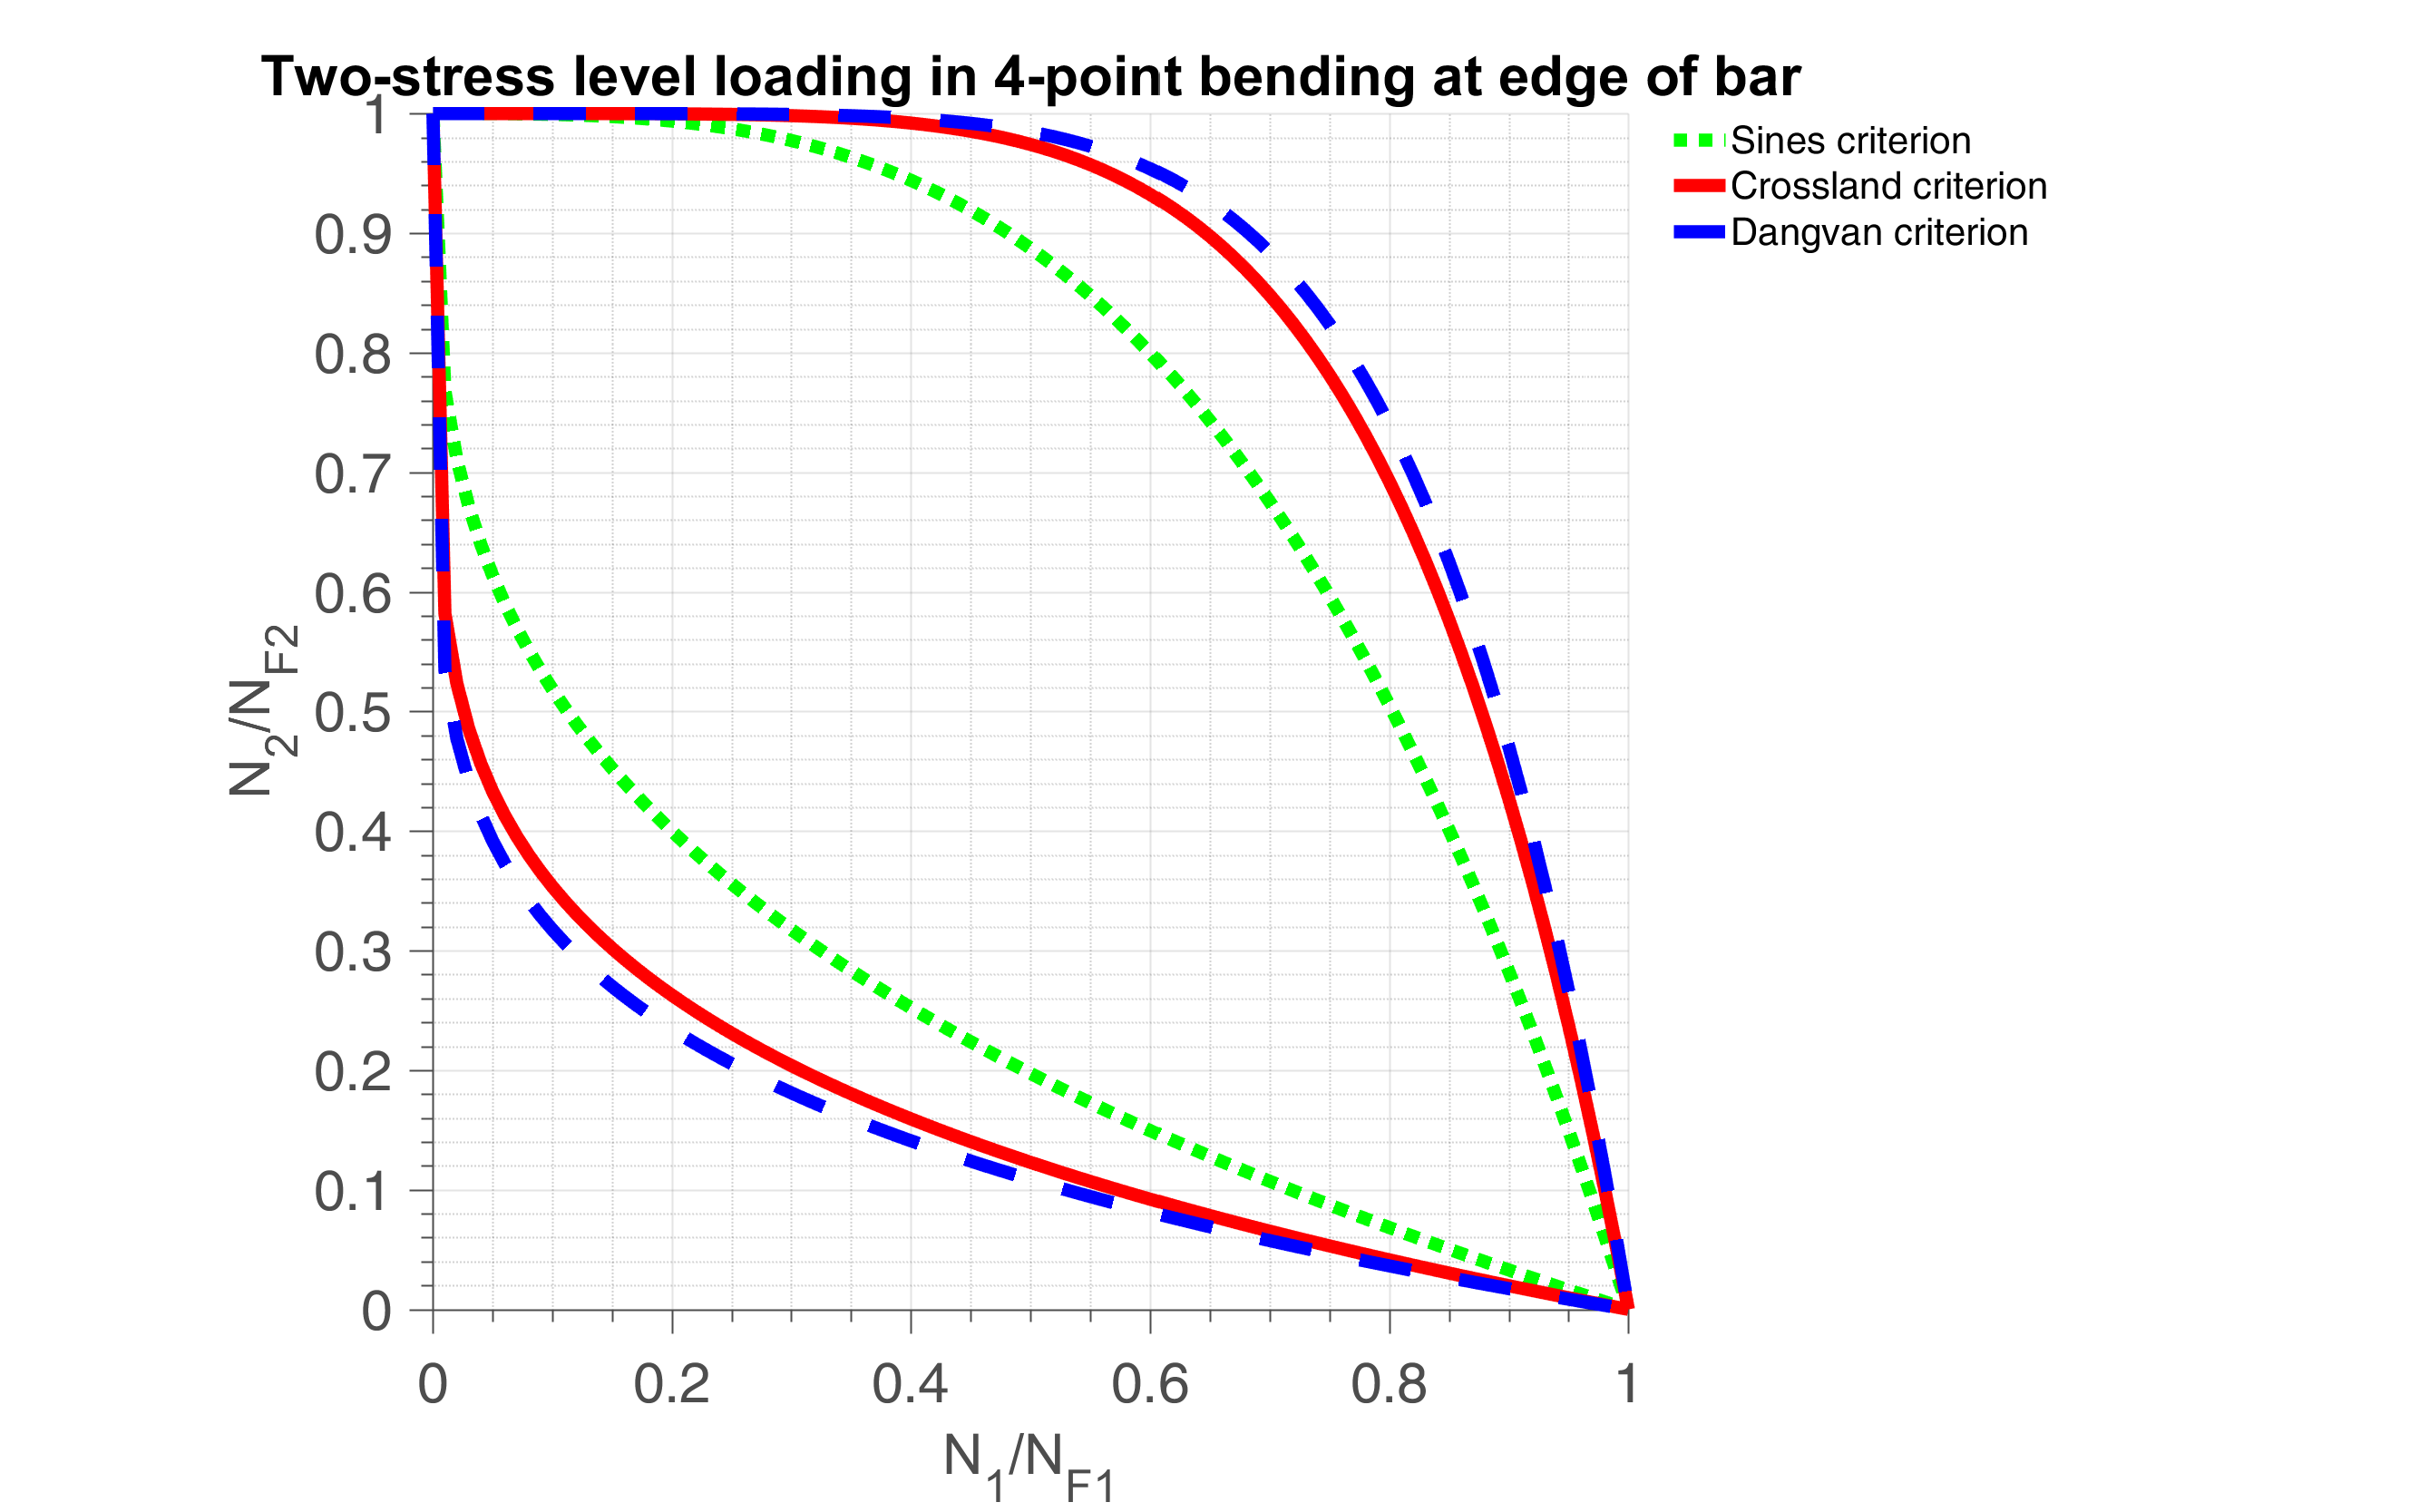
\includegraphics[width=\textwidth]{figures//2stressB.png} 
	\caption{Two-stress level loading in 4-point bending at y=3}
	\label{2stressB}
\end{figure}

\newpage
\subsection{Test on rotative bending}
From the fatigue zone we select $r=0.5$ as the radius to study. 
The $A_{\uppercase\expandafter{\romannumeral2}}-N_F$ figure is shown in \figref{JNRB}.

\begin{figure}[h!]
	\centering
	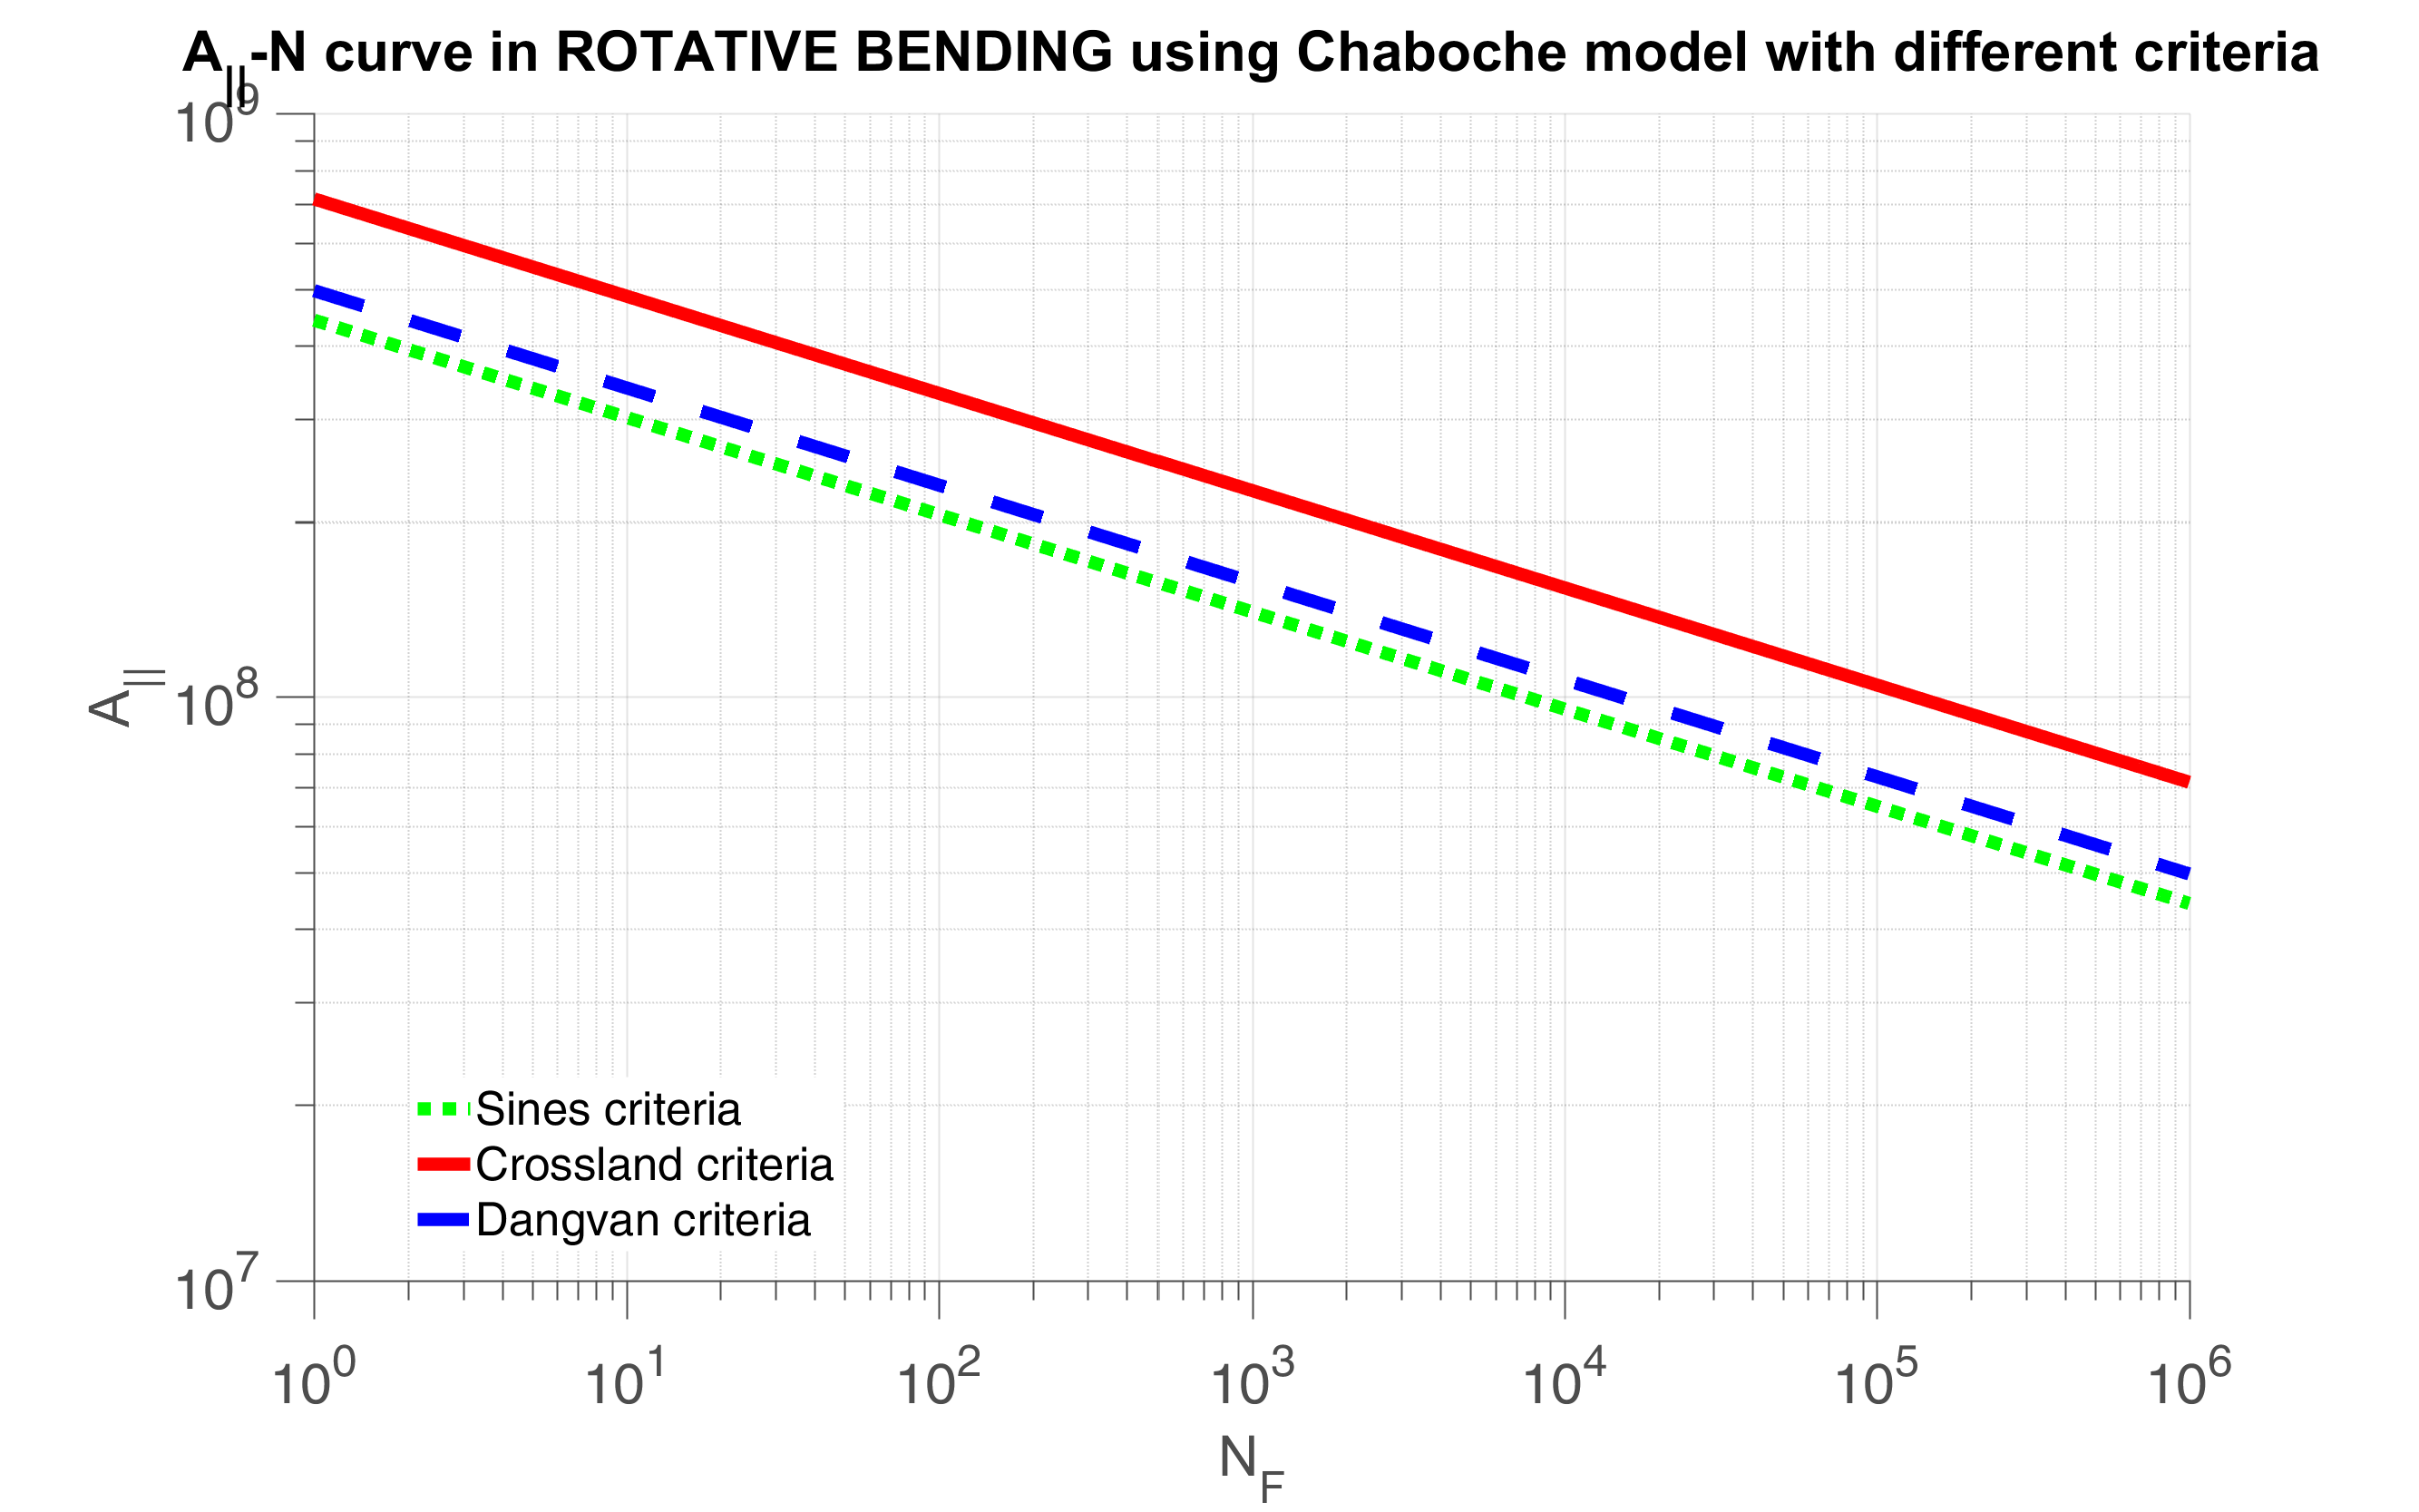
\includegraphics[width=\textwidth]{figures//JNRB.png} 
	\caption{$A_{\uppercase\expandafter{\romannumeral2}}-N_F$ curve in rotative bending at r=3}
	\label{JNRB}
\end{figure}

In rotative bending,we assume the rotating speed are $w=5rpm$. The applied force are respectively $F=9E5 N$ and $F=3E5 N$. We select:

$s_{-1}=f_{-1}=400MPa$, $\sigma_{u}=1000MPa$

\vspace{6pt}
$\sqrt{J_{2a_1}}=7.0226E8 Pa$

\vspace{6pt}
$\sqrt{J_{2a_2}}=6.6454E8 Pa$

\vspace{6pt}
$P_{m_1}=6.8921E8 Pa$

\vspace{6pt}
$P_{m_2}=7.1700E8 Pa$

Substituting the above to Eq.\eqref{eq.eta} we can get $\eta$ in High-Low sequence:
and in Low-High sequence as shown in Table.\ref{tab.etarb}:
\begin{table}[!h]
	\centering
	\begin{tabular}{llll}
		\hline
		$\eta$ value   & Sines  & Crossland & Dang Van \\ \hline
		High-low & 0.7170 &  0.7392 &   0.6608   \\
		Low-high & 1.3947 & 1.3528   &  1.5133  \\ \hline
	\end{tabular}
	\caption{$\alpha$ induced sequence effect parameter $\eta$ value with different criteria in rotative bending}
	\label{tab.etarb}
\end{table}

The predicted results are shown in \figref{2stressRB}.

\begin{figure}[h!]
	\centering
	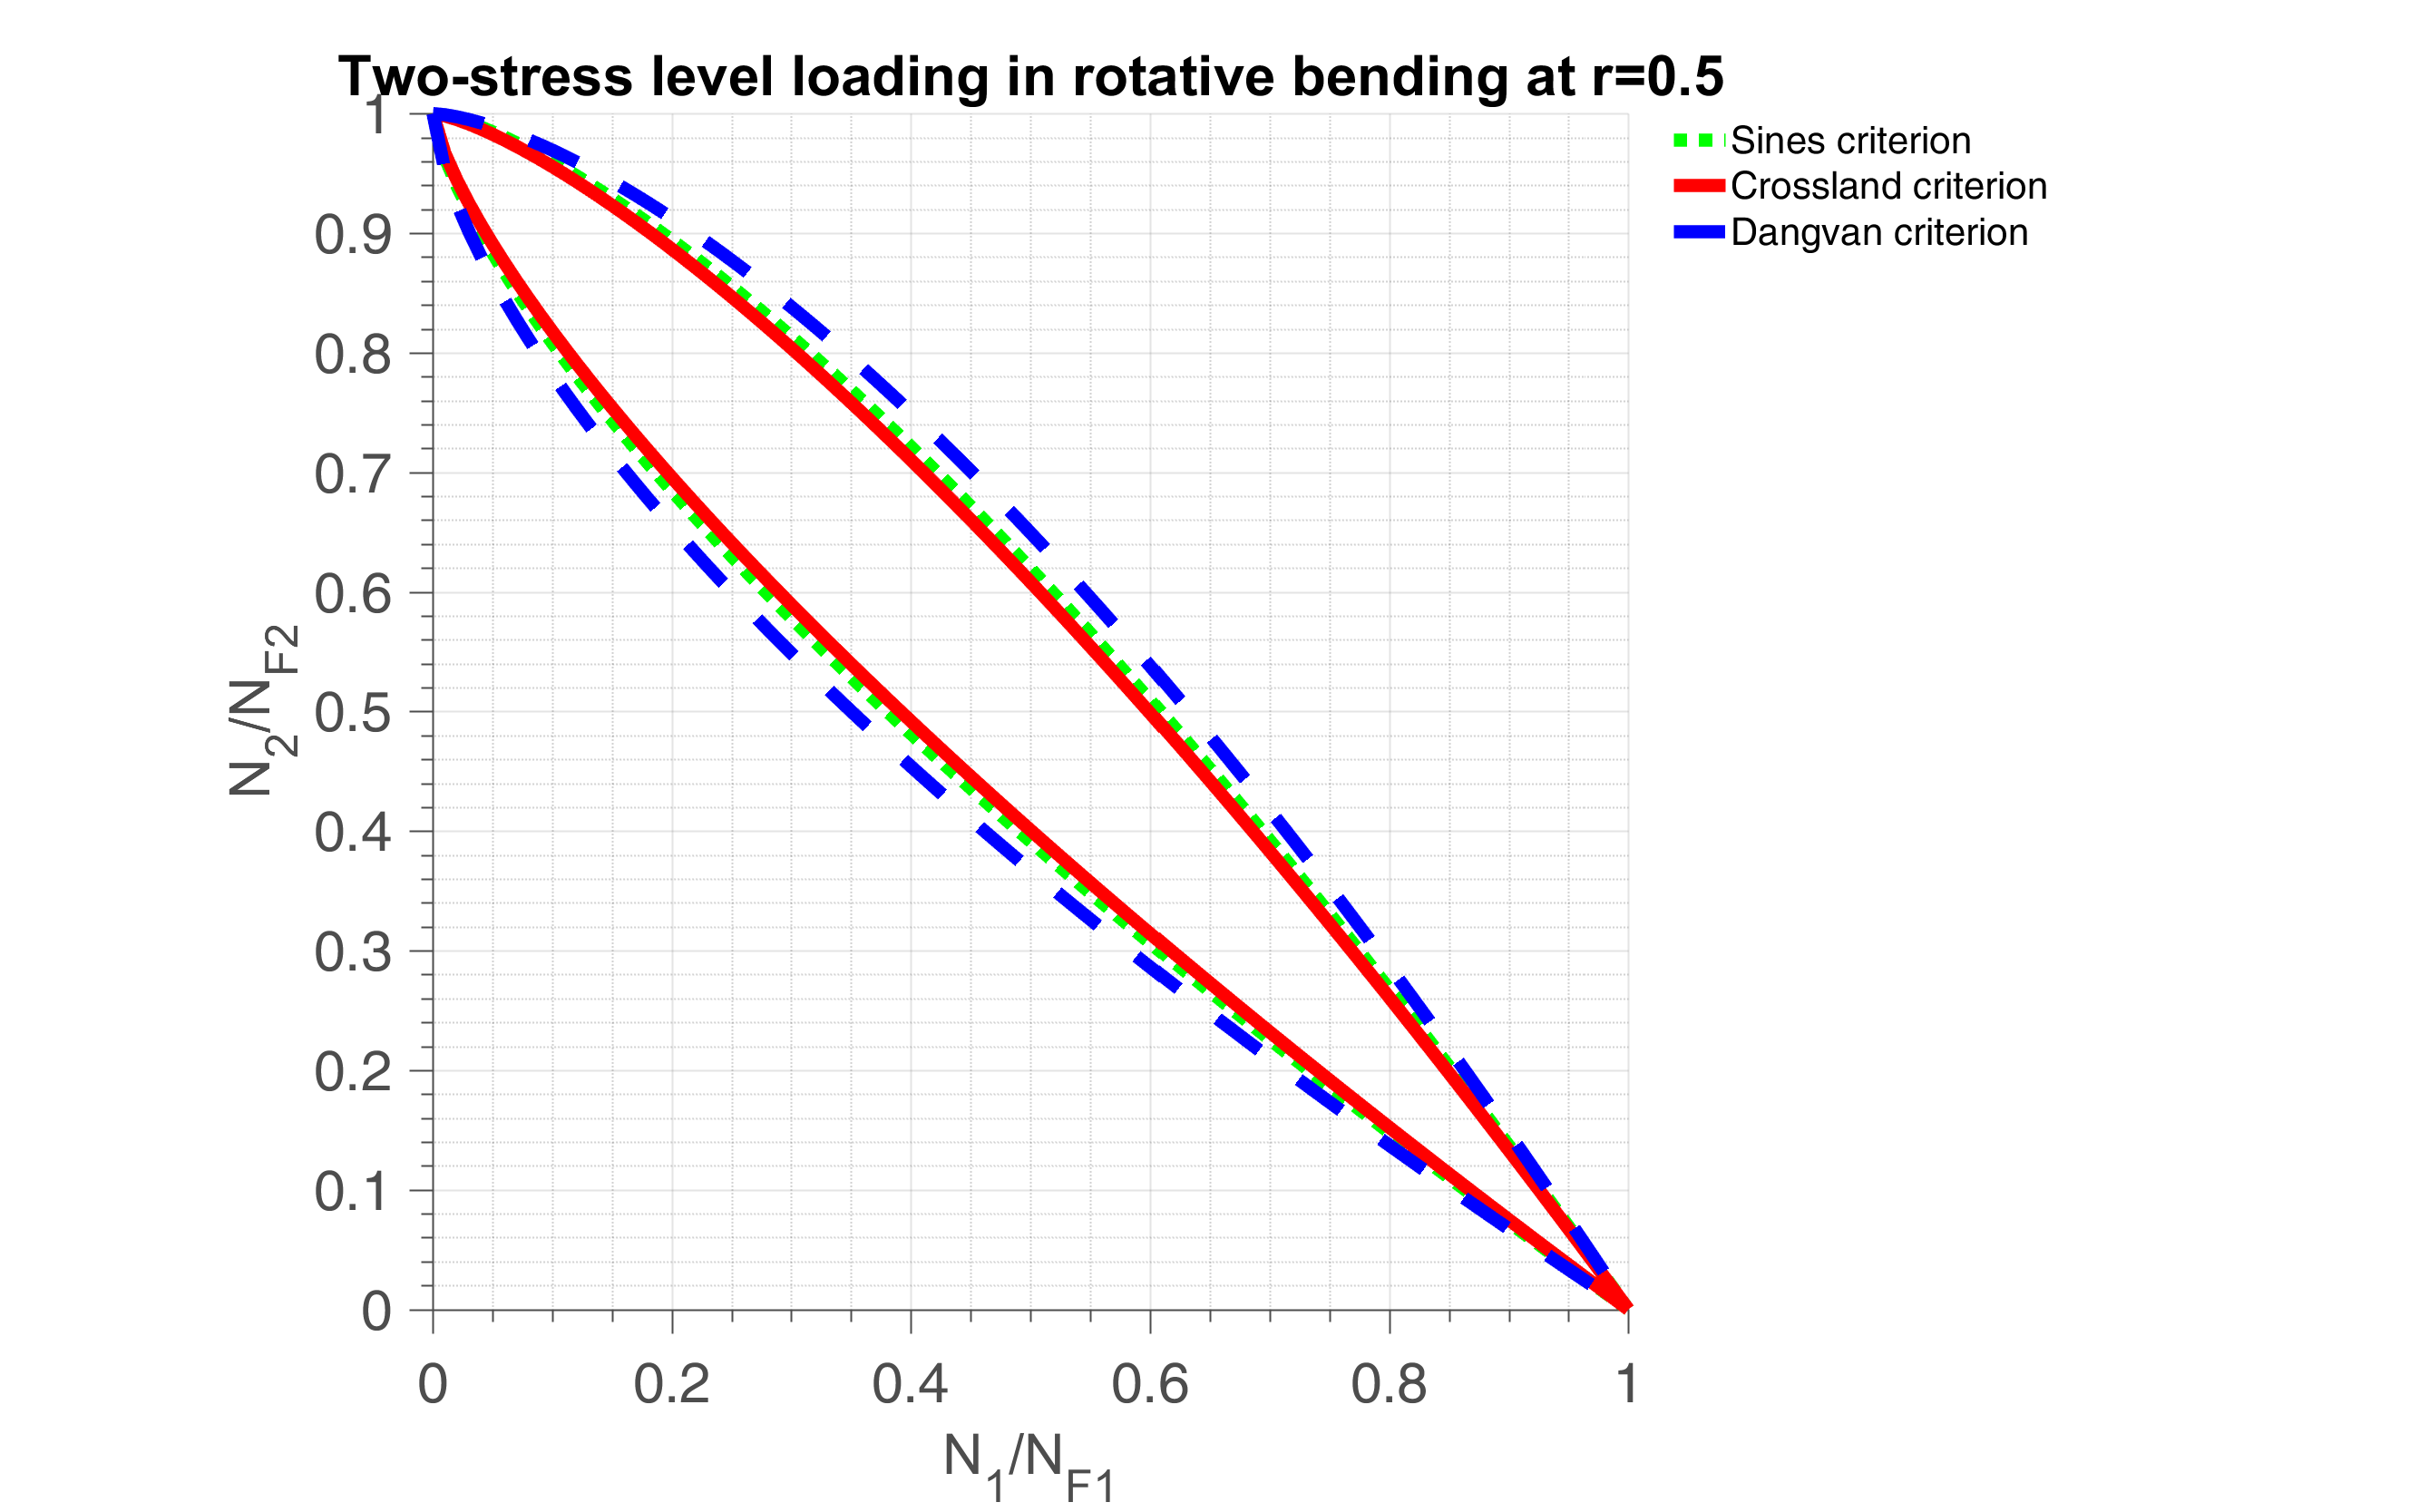
\includegraphics[width=\textwidth]{figures//2stressRB.png} 
	\caption{Two-stress level loading in rotative bending at r=0.5}
	\label{2stressRB}
\end{figure}
\clearpage

\textbf{Discussion}

The Chaboche law is based on this assumption: fatigue damage occurs and accumulates only when the loading stress is higher than its fatigue limit. However, Eq.\eqref{chabochemulti} neglects the damage contribution of the loading stress which is lower than the fatigue limit. According to some experimental results such as: Lu and Zheng \cite{xi2008strengthening} \cite{xi2009strengthening} \cite{xi2009changes}, Sinclair \cite{sinclair1952investigation}, and Makajima et al. \cite{nakajima2007coaxing}, it has shown that the damage of low amplitude loads is one
of the main reasons for prediction errors. 

Impurities in the material affect the fatigue life. So does the material's hardness, and especially its surface condition. How the components were heat-treated in the factory is another factor. The operating temperature makes a difference, too. Worse still is the structural component's shape: notches and sharp corners create concentrations of stress that can initiate cracks. Thus further studies should be carried out concerning these factors.

\section{Cycle Counting Method}
\label{sec:5.1}
Whatever damage accumulation law is used, whatever fatigue criterion is used(Sines, Crossland, Dang Van,...), up to now all fatigue prediction which have been presented are based on the notion of cyclic loads of different amplitudes applied successively. How do we identify those cycles in a random loading history?

In this framework, a counting method is a method for identifying a statistical event
in a random loading sequence. This event can be, for example, extrema,
ranges or cycles of the signal. A method of counting stress cycles determines
therefore the number or the density of presence of the stress cycles in the loading signal.
In other words, the counting method consists in discretizing the loading sequence
variable in simple elementary cycles easy to implement in any forecasting process
of fatigue life. Indeed, each elementary cycle, extracted from the sequence of
load, is denoted by its amplitude and its mean value to which corresponds one
well-defined lifetime. Then, the elementary damage of the extracted cycle is calculated using
a rule of damage. The process repeats along the sequence studied to evaluate
the total damage by means of an accumulation law, and consequently to determine the number of
sequences at break.

Some methods of counting have been developed by the experts. They all lead to different results and therefore, for some, to errors in the calculation of the duration of life. We can cite by way of example six major families of counting techniques,
described in various works \cite{ASTM1985}:

\vspace{6pt}
\noindent
- the counting of the loading time,\\
- the counting of extrema between two passages by the mean value,\\
- the counting of areas,\\
- the counting of paired ranges,\\
- the counting of overflows,\\
- rainflow cycle counting, say ``the drop of water."
\vspace{6pt}

The object of all cycle counting methods is to compare the effect of variable amplitude load histories to fatigue data and curves obtained with simple constant amplitude load cycles. Rainflow counting is a process to obtain cyclic data of complex loading. Its name comes from the original description from the Japanese researchers Matsuiski and Endo where they describe the process in terms of rain falling off a pagoda style roof. A more insightful description based on cyclic plasticity is usually used to explain the method.

\begin{figure}[h!]
	\centering
	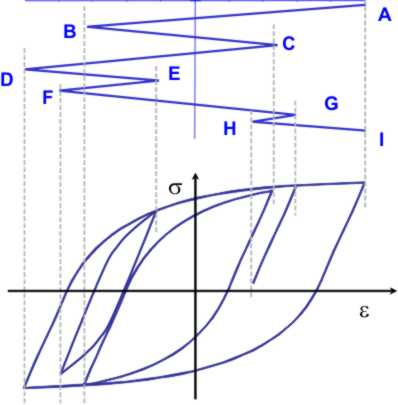
\includegraphics[width=0.4\textwidth]{figures//rainflow.jpg} 
	\caption{Complex Cyclic Loading}
	\label{rainflow}
\end{figure}

In \figref{rainflow}(retrieved from https://www.efatigue.com/variable/background/rainflow.html) a simple loading history ( points A - I ) is plotted vertically so that it resembles a Japanese pagoda. The resulting deformation, stresses and strains, is plotted directly below the loading history. In the lower part of the figure, four cycles are easily identified. One large overall cycle, one intermediate cycle in the center of the plot, and two smaller cycles. Each cycle has its own strain range and mean stress. From a deformation viewpoint the process proceeds as follows. Start at A, the maximum strain, and unload the material to B. Then reload to point C and unload to D. When the material reaches the strain at point B during the unloading from C to D the material remembers its prior deformation and deforms along a path from A to D as if the event C-D never happened. This is better illustrated in the next part of the loading. Load from D to E and unload to F. Now load from F to G. When the material reaches the strain at point E during the loading from F to G the material remembers its prior deformation and deforms along a path from D to G as if the event E-F never happened. The same process occurs for G-H.

Rainflow counting will identify four cycles, A-D-I, B-C-B, E-F-E and G-H-G. Rainflow counting identifies the major load excursions, for example D to I, and treats subcycles like E-F and G-H as interruptions to the overall loading event D-I.

\vspace{6pt}
The five-step procedure to extract the cyclic data is summarized as follows:

1.  Determine the peaks and valleys of the stress/strain during cycling, and in order to start from the absolute maximum (\figref{Reorder}).

2.  Visualize as draining water from the deepest valley (\figref{StressRange}).

3.  Measure total depth drained (stress range) and mean depth (mean stress) of this valley, (\figref{StressRange}), and the number of these cycles in the load history. 

4.  Continue by draining the next lowest (\figref{DrainWater}) and repeat until all valleys are drained. A  Rainflow  cycle is counted if the second segment is vertically shorter than the first and the third segments(i.e. 6-7 is smaller than 5-6 and 7-8).

5.  Use the damage rule to obtain the life from all cycles.

\begin{figure}[h!]
	\centering
	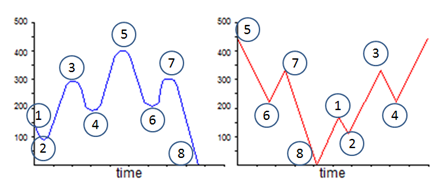
\includegraphics[width=0.6\textwidth]{figures//Reorder.png} 
	\caption{Reorder to Start from Absolute Maximum(retrieved  from ``How to Calculate Fatigue Life When The Load History Is Complex'', February 13, 2015, author: Michael Bak, https://caeai.com/blog/how-calculate-fatigue-life-when-load-history-complex)}
	\label{Reorder}
\end{figure}

\begin{figure}[h!]
	\centering
	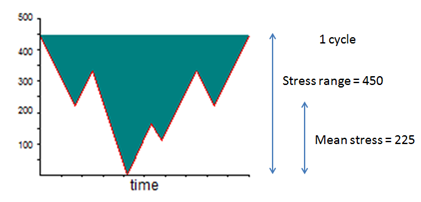
\includegraphics[width=0.6\textwidth]{figures//StressRange.png} 
	\caption{Imagine Filling with Water and Extract Stress Range and Mean Stress(retrieved  from ``How to Calculate Fatigue Life When The Load History Is Complex'', February 13, 2015, author: Michael Bak, https://caeai.com/blog/how-calculate-fatigue-life-when-load-history-complex)}
	\label{StressRange}
\end{figure}

\begin{figure}[h!]
	\centering
	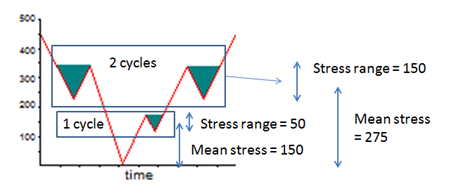
\includegraphics[width=0.6\textwidth]{figures//DrainWater.png} 
	\caption{Drain Water Starting at Lowest Valley and Repeat Cycle Extraction(retrieved  from ``How to Calculate Fatigue Life When The Load History Is Complex'', February 13, 2015, author: Michael Bak, https://caeai.com/blog/how-calculate-fatigue-life-when-load-history-complex)}
	\label{DrainWater}
\end{figure}   

\begin{figure}[h!]
	\centering
	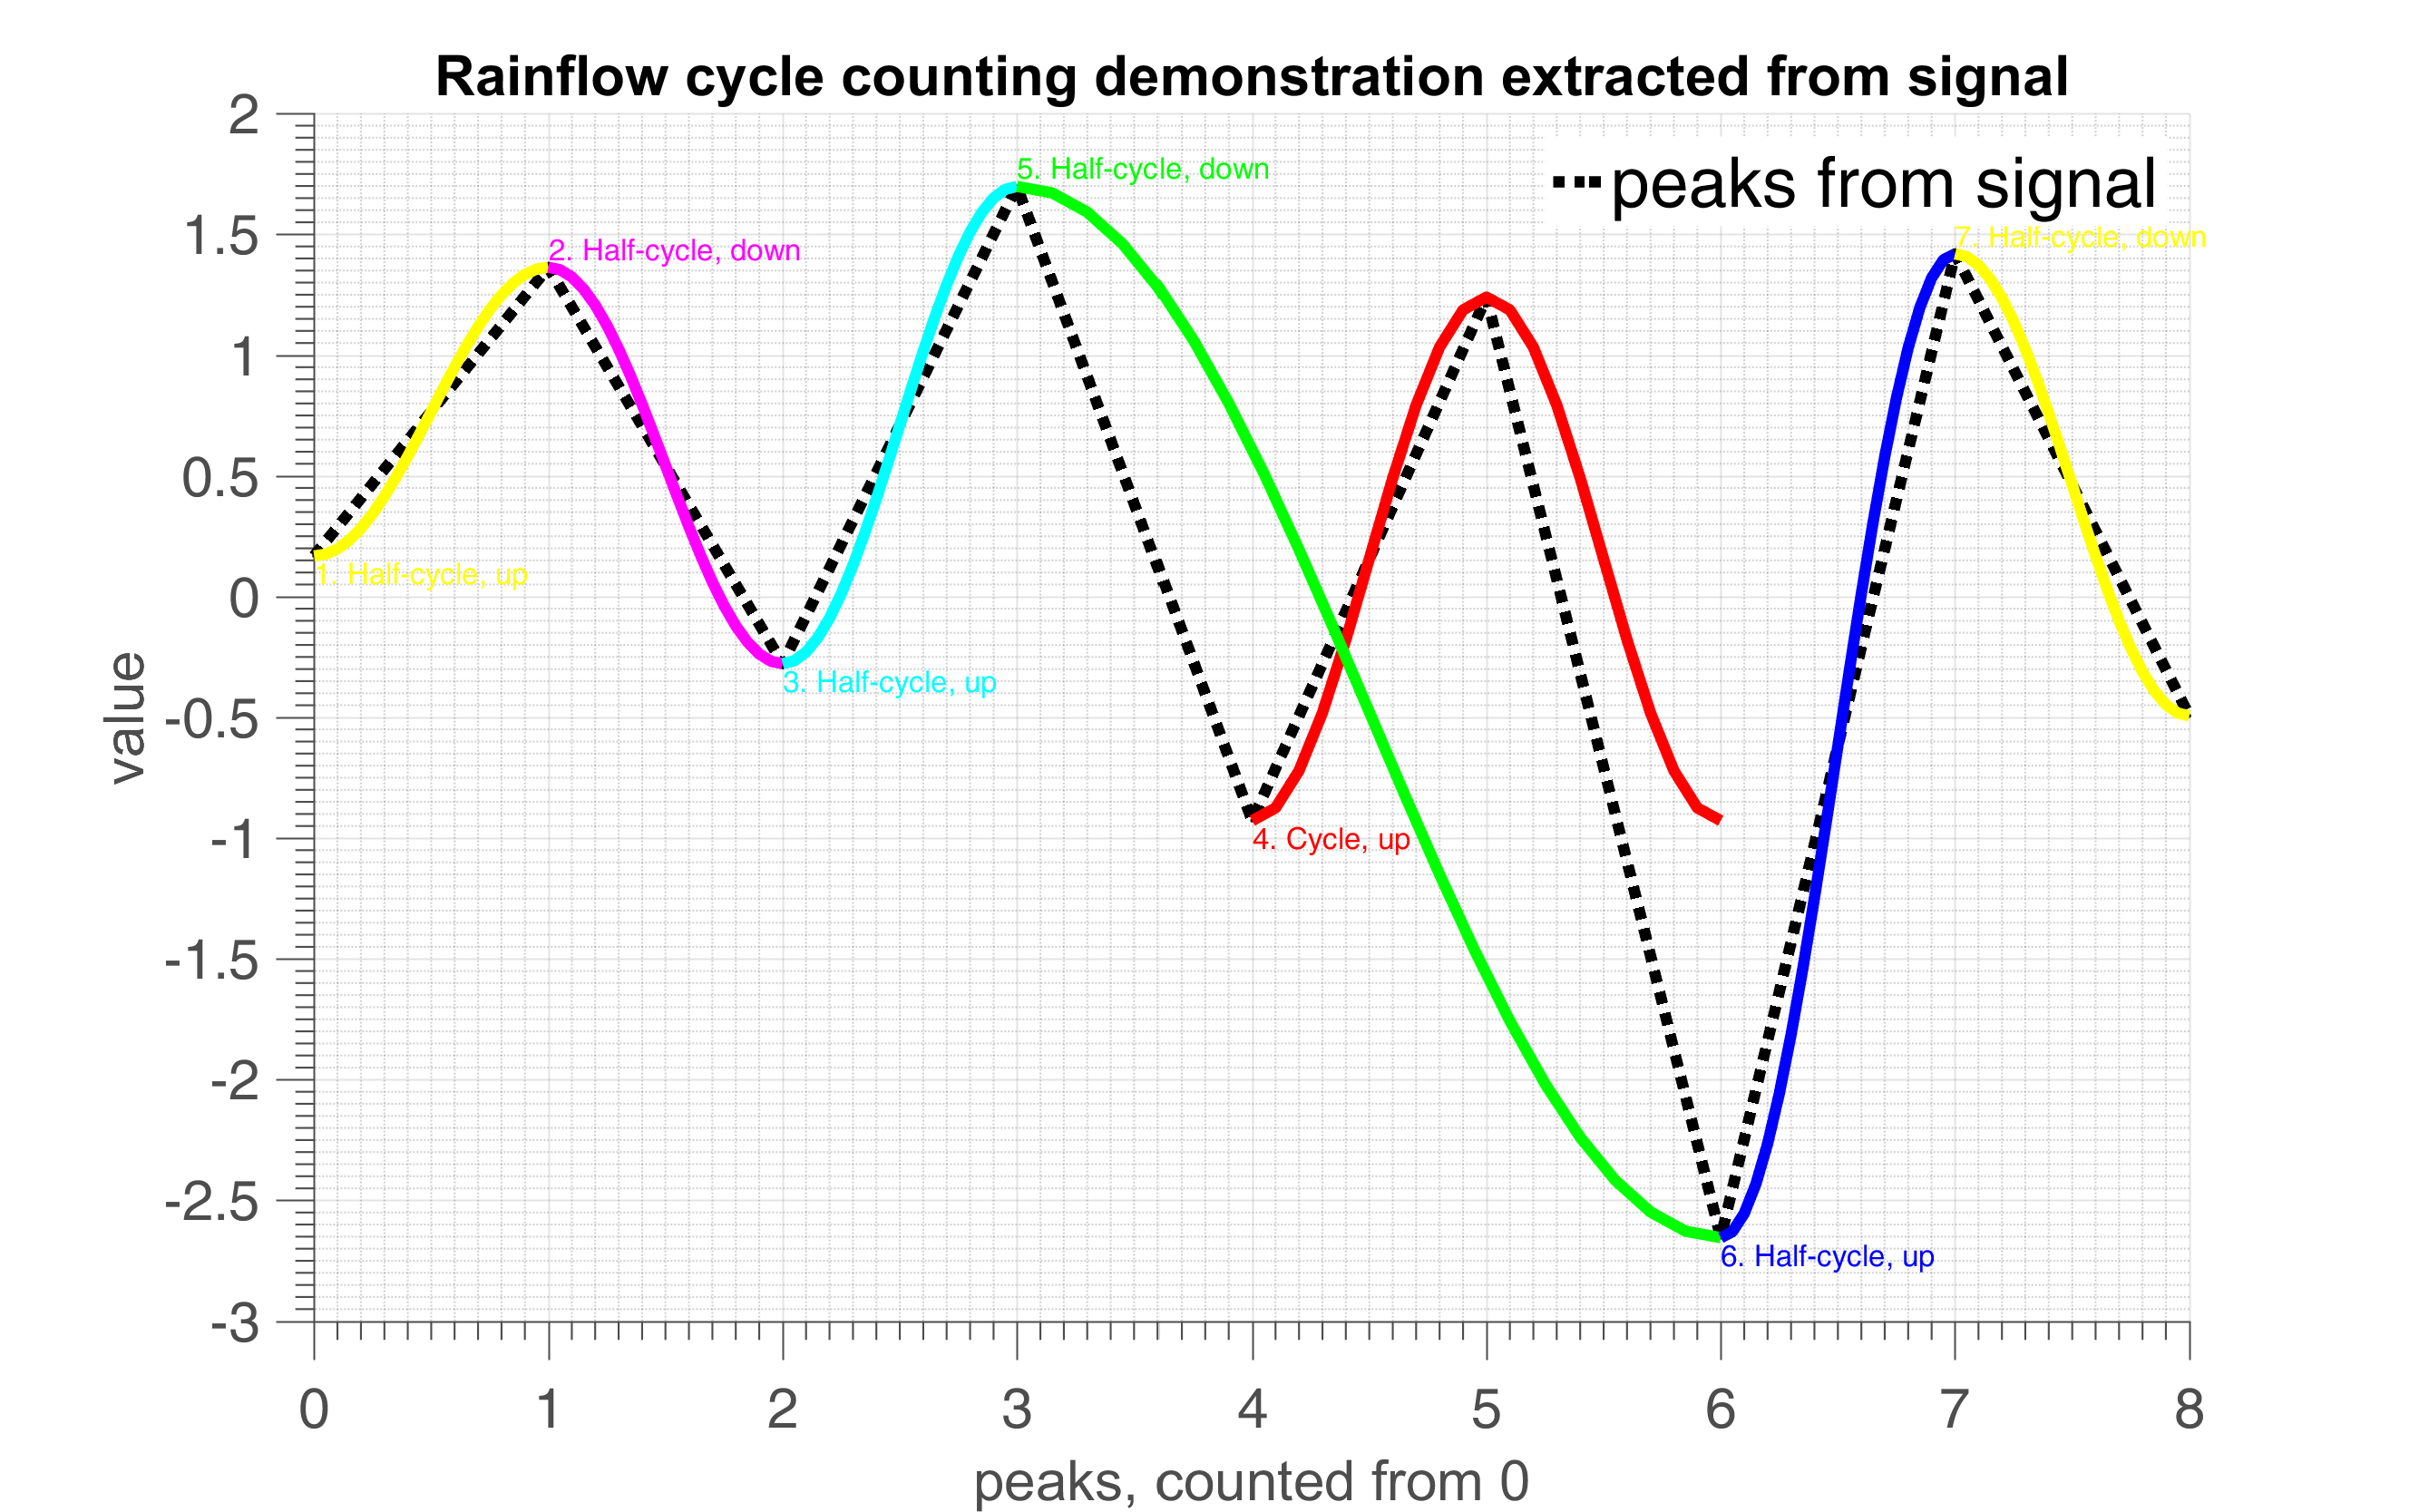
\includegraphics[width=\textwidth]{figures//rfdemo.png} 
	\caption{Rainflow counting method demonstration}
	\label{rfdemo}
\end{figure}  

Once all the cycles have been categorized, the Palmgren-Miner Rule is applied. Even though the linear damage rule ignores sequence effects, it is most widely used because of its simplicity and the fact that though many nonlinear damage models have been developed, unfortunately none can encompass many of the complicating factors encountered during complex variable amplitude loading. As an example, for this case assuming mean stress is ignored:

$$\sum_i \frac{N_i}{N_{F_i}}=\frac{1}{N_{F_{450}}}+\frac{1}{N_{F_{200}}}+\frac{1}{N_{F_{50}}}+...=1.$$

where n is replaced with the number of actual cycles of its corresponding type in the load history, for instance $N_{F_{450}}$ represents the life obtained from the $S-N$ data for a stress range of $450MPa$.  From this equation, the number of total cycles through the entire load history can be found.

The rainflow procedure can be automated so that cyclic content of complex loading can be extracted efficiently.  For example, fatigue computer codes such as $nCode DesignLife$ will accept files of test data, or the input of multiple load steps from a static or transient finite element analysis, and use the rainflow approach to automatically extract the cyclic data.  In addition, $DesignLife$ automates the Palmgrem-Miner Damage Rule calculation to determine number of cycles to failure, with the term cycle here defined as one pass through the entire time history. A computer program that accomplishes rainflow cycle counting applied to a complex history such as that in \figref{loadhistory} results in a table of ranges and means shown in \figref{loadhistory1}.

\begin{figure}[h!]
	\centering
	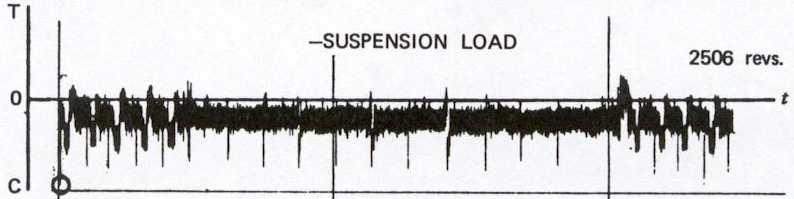
\includegraphics[width=0.9\textwidth]{figures//loadhistory.png} 
	\caption{Suspension load}
	\label{loadhistory}
\end{figure}

\begin{figure}[h!]
	\centering
	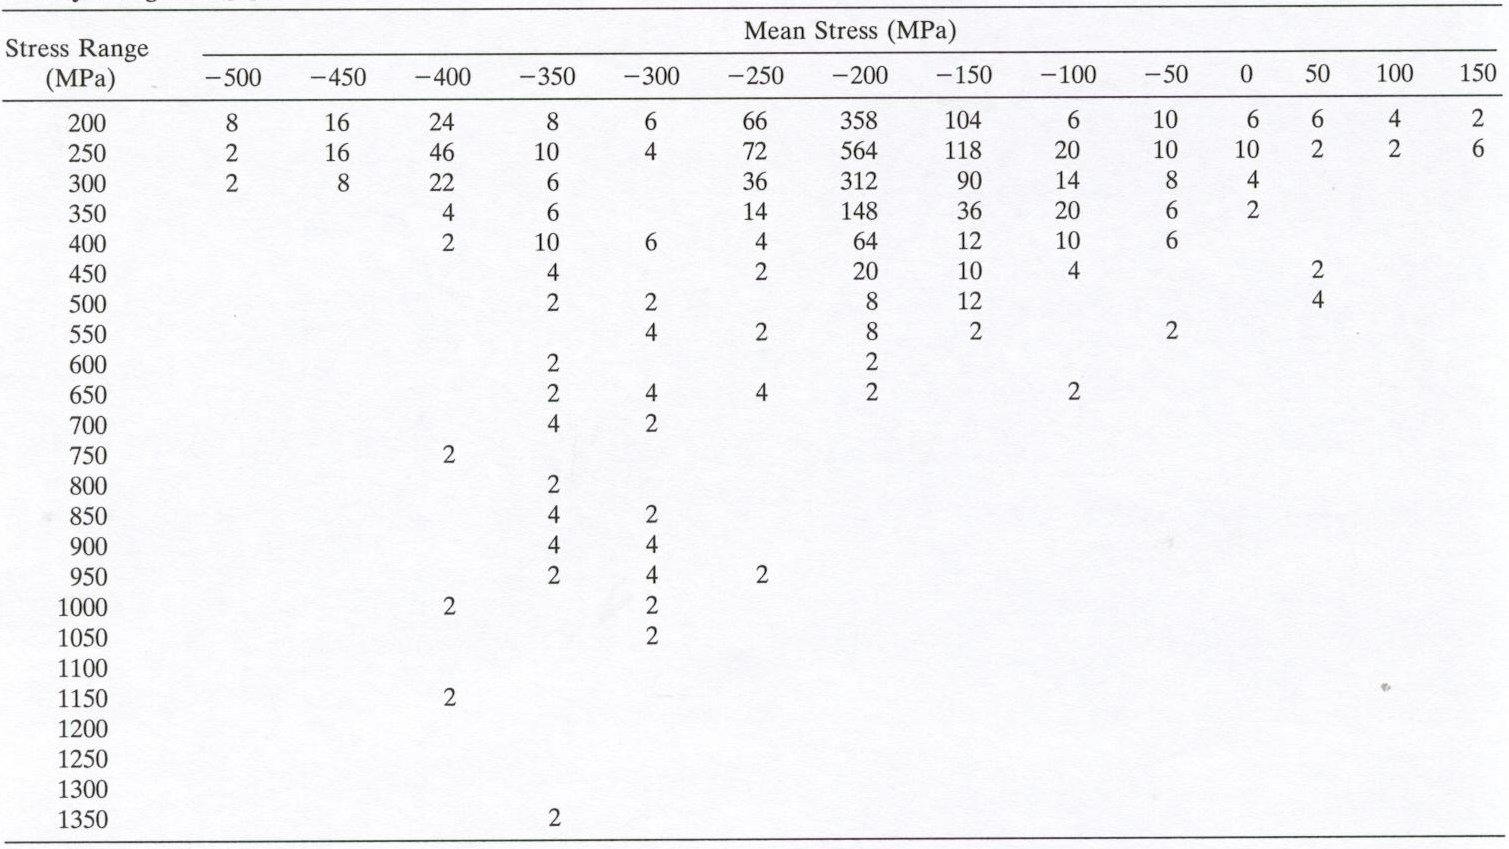
\includegraphics[width=\textwidth]{figures//loadhistory1.png} 
	\caption{Example of the Number of cycles at Various Stress Ranges and Mean Stress Combinations from the Suspension Load History in \figref{loadhistory}}
	\label{loadhistory1}
\end{figure}




 %chaboche part
%%!TEX root=../Thesis_Zepeng.tex
\chapter{Handling general loadings}\label{chp:5}
\minitoc

\section{Multiscale energy dissipation approach}
\label{sec:5.1}
Fatigue failure is a damage accumulation process in which material property deteriorates continuously under fatigue loading and the damage depends on the size of stress and strain. With the accumulation of fatigue damage, some accidents occur for these components. Thus, it is important to formulate an accurate method to evaluate the fatigue damage accumulation and effectively predict the fatigue life of these components even when subjected to complex loadings.

The problem is then to define criteria able to predict this endurance limit. The micro-macro approach applied to the field of endurance was born with the work of \cite{van1973khmu}, and since it has been used many times, including by \cite{papadopoulos2001long} to take better account of loading path effects. For simplicity and to avoid too costly identification procedures of fatigue data, criteria are often expressed using two parameters. The first relates generally to a shear stress $\tau$ (on a plane or on average over an elementary volume) while the second $\sigma$ reflects the normal stress effects (mean and amplitude) often through the hydrostatic stress are the most numerous (\cite{crossland1956effect}, \cite{sines1959behavior}, \cite{FFE:FFE452}, \cite{thu2008effet}).  The normal stress acting on the material plane is sometimes defined from a critical plane(\cite{findley1959}), or through integration at every plane of an elementary volume(\cite{liu1993berechnung}).  In particular, a probabilistic approach based on this type of integration is proposed in \cite{thu2008effet} .

Other authors use energy based approaches. \cite{ellyin1974criterion} is one of the first to propose a fatigue criterion based on cyclic shear deformation energy. This approach was taken up and complemented by \cite{lefebvre1981cognitive} and \cite{ellyin1991phase} for the case of multiaxial loadings. In France, this approach is reflected in the work of \cite{Froustey1992} and then in \cite{palin1996fatigue} and \cite{banvillet2001prevision}. In recent years, a new class of criteria coupling mesoplasticity and damage has also emerged. In \cite{lemaitre1999two}, for example, the author use the approach introduced by \cite{lemaitre1985mecanique} based on the thermodynamics of irreversible processes and the mechanics of continuous media.   Models based on plasticity-damage coupling were also proposed in \cite{flaceliere2004contribution},\cite{monchiet2006contributions}. In the case of fatigue, we usually employ in this damage framework the concept of the loading cycle instead of time to evaluate the evolution of damage and to measure the fatigue lifetime. The equations then depend on the load through globally defined quantities over a cycle, such as amplitude, maximum value, mean value. The growth equation of fatigue damage is therefore taken in the form as described in Chapter \ref{chp:4}:
$$\delta D=f(D)\delta N$$
$$\delta N=f_n\delta t$$
where $\delta t$ is a time sampling of the history in a given number of time intervals $\delta t_1,\delta t_2 ... \delta t_i, ...$ and $f_n$ is the mean frequency of those cycles during the considered time step.

The problem in these approaches is then to take into account the presence of complex variations of the stress tensor. Heuristic formulations with different multiaxial fatigue criteria have been proposed, but most of them still requires the notion of load cycles. The objective of the present chapter is to contribute to the development of life models that take into account such complex variations while avoiding the notion of load cycle. Our fundamental thought is to assume within a micro-macro approach that the local dissipated energy at small scale contributes to the damage which governs fatigue at failure. We follow the Dang Van paradigm. The structure is elastic  at the macroscopic scale. At each material point, there is a stochastic distribution of weak points which will undergo strong plastic yielding, which contributes to energy dissipation and cause damage, without affecting the overall macroscopic stress.

Our model considers a plastic behavior at the mesoscopic scales  with a dependence of the yield function not only on the deviatoric part of the stress but also on the hydrostatic part. A kinematic hardening under the assumption of associative plasticity is also introduced.

Instead of using the number of cycles, we will use in addition as in \cite{lemaitre1999two} the concept of nonlinear damage accumulation during the loading history. To approach real life loading history more accurately, non-linear damage accumulation laws are also considered in our model to take into account the sequencing effect. Fatigue will then be determined from the energy plastically dissipated at all scales during plastic shakedown cycles and from a phenomenological fatigue law linking damage evolution and accumulated mesoscopic plastic dissipation.

The chapter is organized as follows. From section \ref{sec:5.1} to \ref{sec:5.3}, we present the existing methods and background of our strategy.  In section \ref{sec:5.4} we propose the notion of weakening scales and multiscale yield function and describe the plastic dissipation resulting from this notion. And in section \ref{sec:5.5}, based on microscopic plasticity we construct the energy dissipation formula. Section \ref{sec:5.6} gives the proposed nonlinear damage accumulation law and summarizes the full model that we propose. Then we combine the energy dissipation law and nonlinear damage accumulation law with its numerical implementation presented in section \ref{sec:5.7}, while section \ref{sec:5.8} is devoted to various validations on typical load histories classically treated in the literature. Parameter identification strategy is presented in section \ref{sec:5.9}.



\section{Kinematic Hardening Models}
\subsection{Linear Kinematic Hardening}
A hardening rule is needed in microplasticiy to
describe the behavior of the
material once it is plastically
deformed or yielded. One possible hardening rule is the
isotropic rule, which assumes
that strain hardening corresponds
to an enlargement of the yield
surface (i.e. an increase in  yield stress )
without change of shape or
position in the stress space. Another is the kinematic rule,
which assumes that strain
hardening shifts the yield surface
without changing its size or shape.
\begin{figure}[h!]
	\centering
	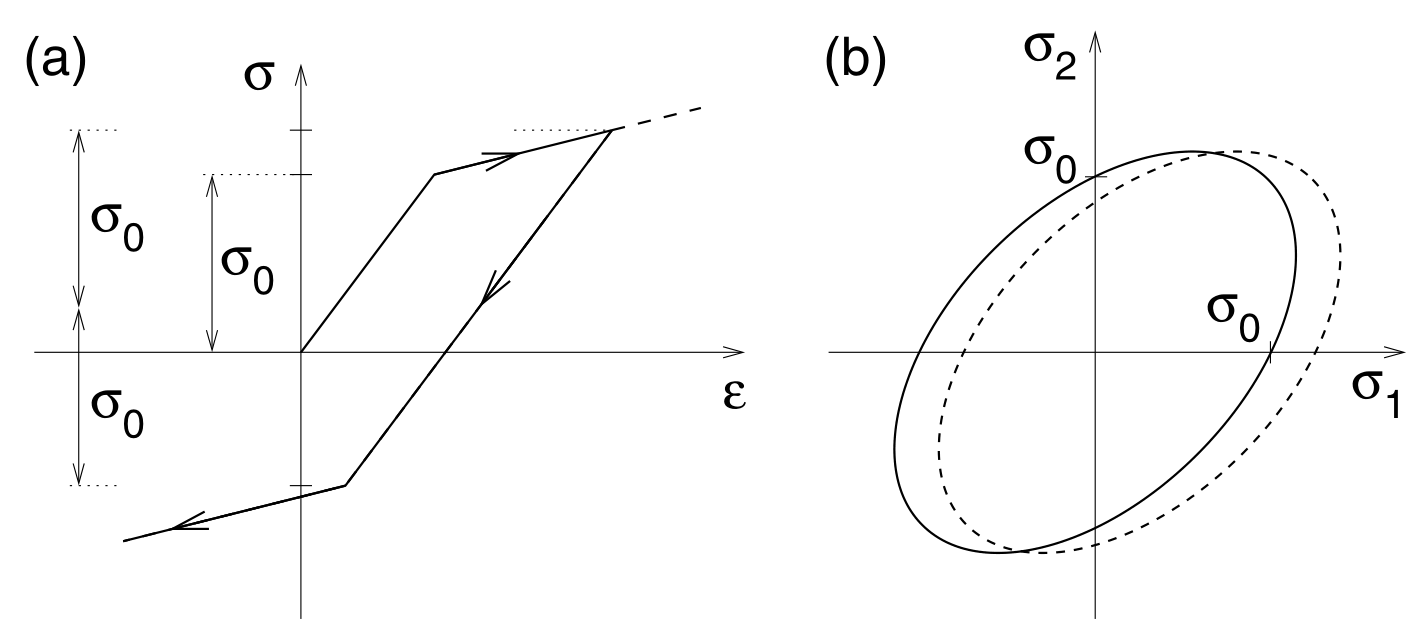
\includegraphics[width=0.8\textwidth]{figures//kinhard.png} 
	\caption{Kinematic hardening: a) uniaxial stress-strain diagram, b) evolution of the
		yield surface in the biaxial stress plane}
	\label{kinhard}
\end{figure}
Kinematic hardening rules are necessary,especially for the case of unloading and cyclic loading.In Kinematic Hardening the current loading surface is assumed not to expand but to move as a rigid body
within the stress space (\figref{kinhard}(b)). The use
of kinematic hardening is, for example, necessary to model the so-called Bauschinger
effect (Bauschinger, 1881). This effect is often observed in metals subjected to cyclic
loading. Even if the magnitudes of the yield stress in tension and in compression
are initially the same, this is no longer the case when the material is preloaded into
the plastic range and then unloaded. For example, after previous yielding in tension,
yielding in compression may start at a stress level lower than the initial yield stress
(\figref{kinhard}(a)).

Kinematic hardening leads to a translation of the loading surface, i.e. to a shift of
the origin of the initial yield surface. If the initial yield surface is described by a yield
function of the form
$$f(\sigma) = F(\sigma) -\sigma_0 $$
the shifted surface is obviously described by
$$f(\sigma,\sigma_b ) = F(\sigma-\sigma_b ) -\sigma_0$$
where $\sigma_b$ is the so-called backstress that represents the center of the shifted elastic
domain and plays the role of a tensorial hardening variable. Now we need a kinematic
hardening law that governs the evolution of the back stress. \cite{melan1938plastizitat} proposed
a law of the form
\begin{equation}
\dot{\sigma}_b =\overline{H}_K \dot{\varepsilon}_p
\label{lineark}
\end{equation}
where $ \dot{\varepsilon}_p$ is the rate of effective plastic strain. According to which the rate of the back stress is proportional to the plastic strain rate. It is a macroscopic variable representing the
dislocation sub-structure resistance to deformation. 
The proportionality factor $\overline{H}_K$ is directly related to the plastic modulus and is derived from a simple
monotonic uniaxial curve.The linear hardening law Eq.\eqref{lineark} is often credited to Prager (1955, 1956); we will call it the Melan–Prager hardening rule. 
\subsection{Non-linear Kinematic Hardening}
%\begin{figure}[h!]
%		\includegraphics[width=\textwidth]{figures//kinehardening.gif} 
%		\caption{Dissipated energy in one cycle and number of cycles %to failure when $\beta=-1$}
%		\label{kinehardening}
%\end{figure}
To describe cyclic plasticity, one of the famous model is the non-linear kinematic hardening model formulated by Armstrong and Frederick. It is based on a physical mechanism of strain hardening and dynamic recovery and is capable of simulating the
multiaxial Bauschinger effect (movement of the yield surface in the stress space). Therefore, the model has been examined and implemented in commercial software and finite element analysis.

The Armstrong-Frederick model (AF) is a modification of the Melan–Prager linear kinematic hardening model. The only modification of this simple model is the "recal" term which changes the evolution law for the symmetric backstress tensor $\sigma_b$ from a classical linear kinematic hardening law (Melan–Prager) to a nonlinear kinematic hardening law. The term is proportional to the current back stress multiplied by the norm of the plastic strain rate. According to the Armstrong-Frederick rule, the evolution of the
back stress is governed by the differential equation:

\begin{equation}
\dot{\bm{\sigma}}_b=\underbrace{\overline{H}_K \dot{\varepsilon}_p}_{lin. kin. hardening} -\underbrace{\gamma\dot{p}\bm{\sigma}_b}_{recall - term, nonlinear hardening}
\label{nonlineark}
\end{equation}
where
$\dot{p}$ is the accumulated plastic strain rate given as $\sqrt{\dfrac{2}{3}}||\dot{\varepsilon}_p||$ . The constants
$\overline{H}_K$
and
$\gamma$
are determined from uniaxial tests.
At the onset of yielding, the
back stress is still zero and Eq.\eqref{nonlineark} gives the same response as the linear hardening
law Eq.\eqref{lineark}. As the back stress develops, the additional term becomes activated and
slows down the rate at which the back stress grows (i.e. reduces the tangent plastic
modulus).

\section{Mean stress effect in local model}
\label{sec:5.3}
Positive mean stress clearly reduces the fatigue life of the material. In design evaluation of multiaxial fatigue with mean stress, a simplified, conservative relation between mean stress and equivalent alternating stress is necessary. We can improve the model by modifying the yield function $\sigma_y$ and the localization tensor in order to take mean stress effect into account.

\vspace{6pt}
\textbf{Christensen approach}
\vspace{6pt}

The yield function that was given by \cite{christensen2000yield} integrates measures of damage, as well as intrinsic yield strength and concept of transitions. The derived yield function formalism resulted in the form as:

\begin{equation}
\frac{\alpha K}{\sqrt{3}}\sigma_{kk}+\frac{(1+\alpha)^2}{2}s_{ij}s_{ij}\leqslant\frac{K^2}{(1+\alpha)}.
\label{eq:yieldfunc}
\end{equation}
Here $\alpha$ changes the shape of the yield function, thus it is called the shape parameter. 
$$\alpha=\frac{\left| \sigma_{11}^C\right| }{\sigma_{11}^T}-1.$$
The new parameter $K$ is called the ideal or intrinsic strength which uniformly expands or contrasts the yield function, thus is is called the scale parameter:
$$K=\frac{(\sigma_{11}^C)^2}{\sqrt{3}\sigma_{11}^T}.$$
The intrinsic strength would occur if there were no damage or microstructure disturbance. 
$\sigma_{11}^C$ and $\sigma_{11}^T$ are respectively compressive and tensile yield stress in uniaxial states where $\left| \sigma_{11}^C\right| \geqslant\sigma_{11}^T$(for ductile materials, $\frac{1}{2}\leqslant\dfrac{\left| \sigma_{11}^C\right| }{\sigma_{11}^T}\leqslant 1$). The yield stress in uniaxial and shear states are given by:

\begin{equation}
\begin{split}
&\sigma_{11}^C=\frac{-\sqrt{3}K}{(1+\alpha)}\\
&\sigma_{12}^Y=\frac{K}{(1+\alpha)^{3/2}} \\
&\sigma_{11}^T=\frac{\sqrt{3}K}{(1+\alpha)^2}.\\
\end{split}
\label{eq:uniyields}
\end{equation}

At $\alpha=0$, relations Eq.\eqref{eq:yieldfunc} and Eq.\eqref{eq:uniyields} show the behavior to be that of purely Mises type. This is taken to be the ideal condition where the intrinsic strength $K$ solely determines the yield strength. As the shape parameter increases beyond the value $\alpha=1$, the yield function behaves in accordance with  a state of increasing crack density or any other physical weakening. The term fracture, as used here for behavior at or near $\alpha=1$, actually corresponds to fracture mechanics for non-interacting cracks. Beyond this range near $\alpha=1$ or $\alpha\to\infty$ has simply been called yield or failure. Parameter $\alpha$ could be easily viewed as a damage measure or microstructure parameter since it represents microstructure changes on any scale that causes deviation from the ideal state. 

It is concluded a decrease in mean stress $\sigma_{kk}$ reduces the effective value of $\alpha$. That is, moving the behavior toward ductile case. Alternatively, increasing the mean stress moves $\alpha$ toward larger values, which is taken to be that of brittle behavior.

The fully expanded form of the yield function Eq.\eqref{eq:yieldfunc} is:
\begin{equation}
\begin{split}
&\frac{\alpha K}{\sqrt{3}}(\sigma_{11}+\sigma_{22}+\sigma_{33})\\
+&(1+\alpha)^2\left[\frac{(\sigma_{11}-\sigma_{22})^2+(\sigma_{22}-\sigma_{33})^2+(\sigma_{33}-\sigma_{11})^2}{6}
+(\sigma_{12}^2+\sigma_{23}^2+\sigma_{31}^2) \right]\\
\leqslant&\frac{K^2}{(1+\alpha)}.\\
\end{split}
\end{equation}

The most compact form of Eq.\eqref{eq:yieldfunc} is:
\begin{equation}
\frac{1}{2}s_{ij}s_{ij}\leqslant\eta K^2,
\end{equation}
where $\eta$ is a nondimensional scaling factor on $K^2$, determined by mean normal stress.
$$\eta=\frac{1-\dfrac{\alpha(1+\alpha)}{\sqrt{3}K}\sigma_{kk}}{(1+\alpha)^3}<1$$


The mean stress $\sigma_{kk}$ has a positive relationship with the shape parameter $\alpha$. We suppose the material endures transition from ductile to brittle when $\alpha$ reaches 1. That means $\alpha$ has a very similar physical meaning with the damage parameter $D$.

\vspace{6pt}
\textbf{The Gerber parabola}
\vspace{6pt}

Several models are available addressing the influence of tensile mean stress on fatigue life. Among these are the Gerber (Germany, 1874), Goodman (England, 1899), and Soderberg (USA, 1930) models.  The modified Goodman criterion is often used as a design criterion because it is more conservative than the Gerber criterion. The use of the Gerber criterion in the determination of member size is generally more computationally  intensive and so rather unattractive for many designers.

The effect of mean stress on the fatigue strength is commonly presented in Haigh diagrams as shown in \figref{haigh}, where $S_a / S_f$ is plotted against $S_m / S_u$ at fatigue limit. $S_a$ is the fatigue strength at a given life under fully reversed ($S_m = 0$,$R = -1$) conditions. $S_u$ is the ultimate tensile strength. $S_f$ is the reversed fatigue strength in absence of mean stress. The data points thus represent combinations of $S_a$ and $S_m$ giving that life. The results were obtained for small unnotched specimens, tested at various tensile mean stresses. The straight lines are the modified Goodman and the Soderberg lines, and the curved line is the Gerber parabola. These are empirical relationships that are represented by the following equations:

\vspace{6pt}
Modified Goodman: $S_a/S_f + S_m/S_u = 1$

\vspace{6pt}
Gerber: $S_a/ S_f + (S_m/ S_u)^2 = 1$

\vspace{6pt}
Soderberg: $S_a/S_f+S_m/S_y=1$

\begin{figure}[h!]
	\centering
	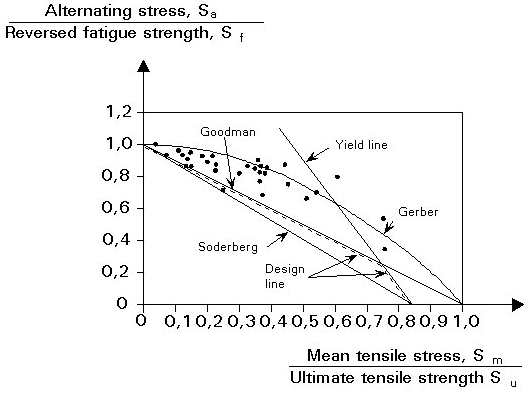
\includegraphics[width=0.8\textwidth]{figures//Gerber.png} 
	\caption{Haigh diagram showing test data points for the effect of mean stress, and the Gerber, modified Goodman and Soderberg relations.}
	\label{haigh}
\end{figure}

In the following section, we introduce the sale dependent mean stress effect in our model.

\section{Weakening scales and yield function}
\label{sec:5.4}
\subsection{The concept of weakening scales} 

We follow the Dang Van paradigm. The structure is elastic at the macroscopic scale. At each material points, there is a stochastic distribution of weak points which will undergo strong plastic yielding, without contributing to the overall macroscopic stress. From a microscopic point of view, there is a distribution of weakening scales, namely $s\in[1,\infty)$. In order to introduce our concept, lest us imagine that we can measure the macroscopic stress intensity at present time by a given value $S_{a}$. Let $\sigma_y$ be the yield limit before weakening. Then we imagine that for a given scale $s$:

\vspace{6pt}
\noindent
$\bullet$ either $1\leqslant s\leqslant \sigma_y/S_{a}$, then $S_{a}\leqslant \sigma_y/s$, the material stays in the elastic regime and there is no energy dissipation at this scale.

\vspace{6pt}
\noindent
$\bullet$ or $\sigma_y/S_{a}\leqslant s\leqslant \infty$, then $S_{a}\geqslant \sigma_y/s$, the material is in plastic regime at this scale, which evolves through kinematic hardening, say from zero initial plastic strain $\uuline{\varepsilon}_p(s)$ and zero initial backstress $\uuline{b}(s)$ at initial time $t_0$. There is then dissipated energy at scale $s$ contributing to the fatigue limit.


\vspace{6pt}

\subsection{Distribution of weakening scales}

We assume the weakening scales have a  probability distribution function following a power law:
\begin{equation}
P(s) = Hs^{-\beta}=(\beta-1)s^{-\beta},
\label{eq.ps}
\end{equation}

where $\beta$ is a material constant. 
The choice of a power law comes with two reasons: on one hand, this type of distribution corresponds to a scale invariant process, on the other hand it leads in cyclic loading to a prediction of a number of cycles to life limit as a power law function of the stress intensity. More general laws can also be proposed, without changing the spirit of the model.

%The integrated probability ranging from macroscopic to microscopic stress  is unity. From this we can conclude:
%$$\int_{1}^{\infty}P(s)ds=\left[ \frac{Hs^{1-\beta}}{1-\beta}\right] _{1}^{\infty}=0-\frac{H}{1-\beta}=1.$$
%Then we know $H=\beta-1$, so the distribution is given by:
%$$P(s) = Hs^{-\beta}=(\beta-1)s^{-\beta}$$
The probability of weakening scales is shown in \figref{ps1} and \figref{ps2}. We can see that smaller $\beta$ leads to larger probability of weakening for large $s$.
\begin{figure}[!h]
\centering
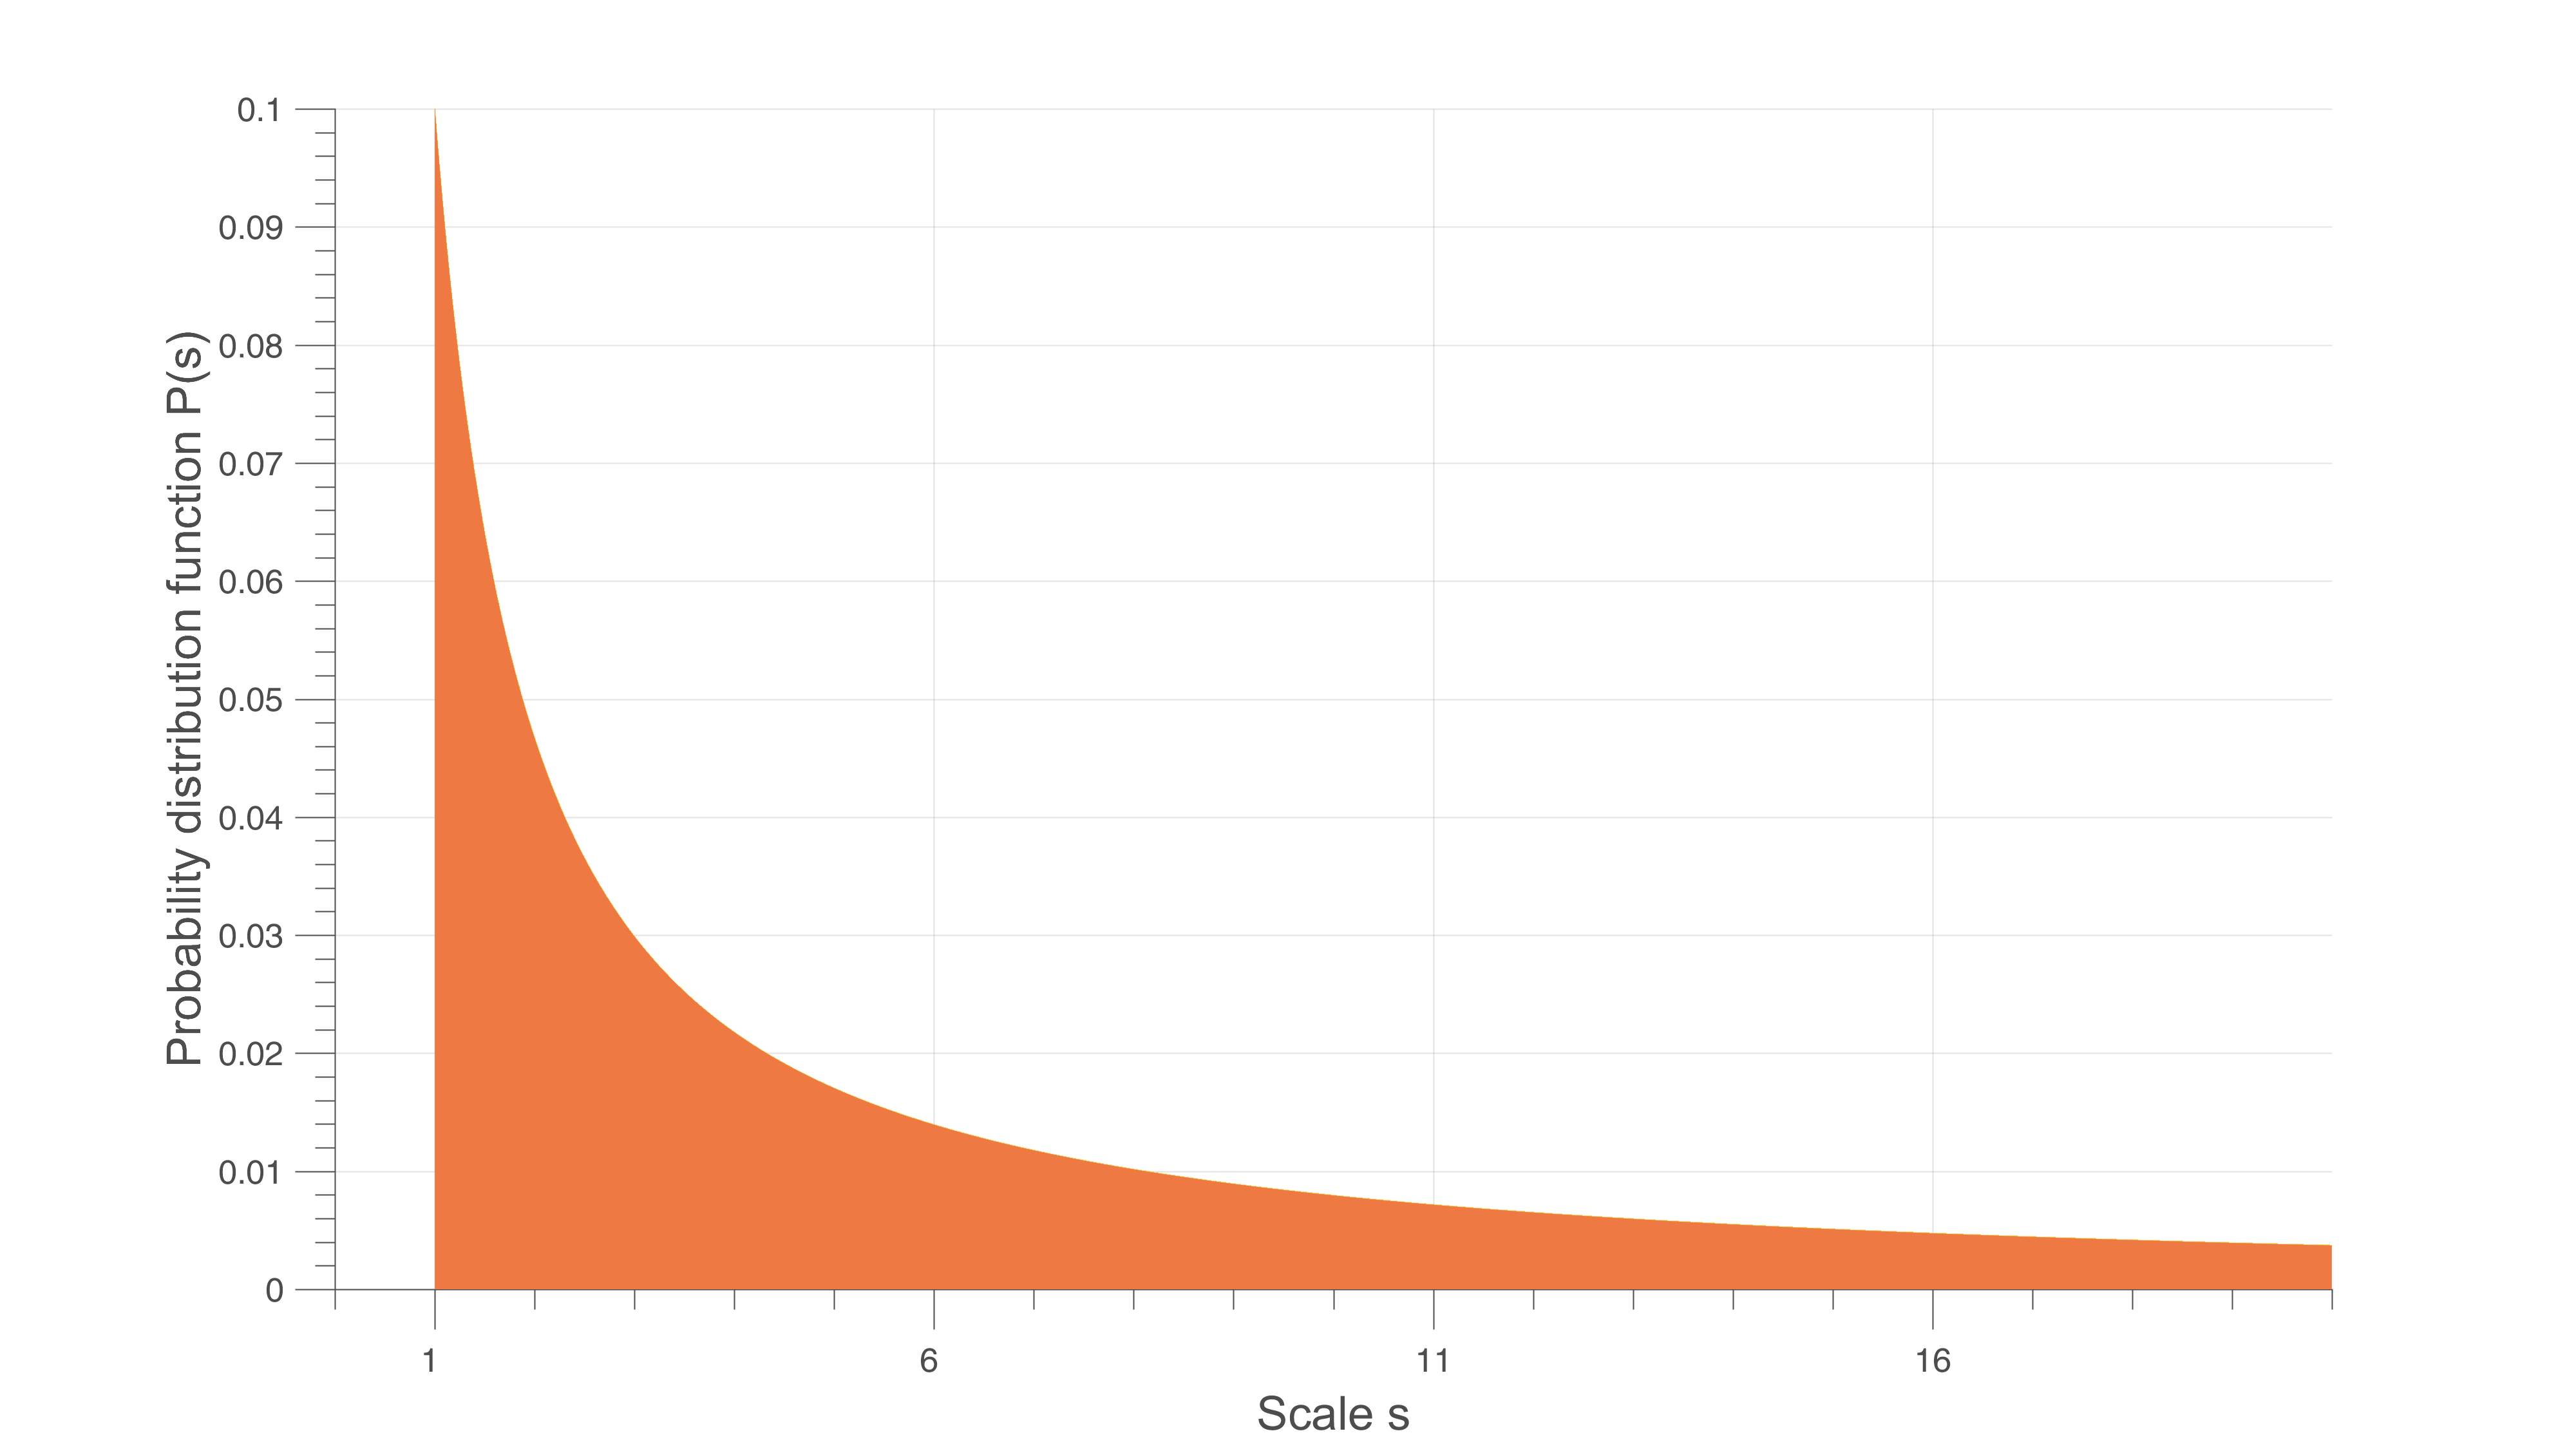
\includegraphics[width=0.9\textwidth]{figures//ps1.png} 
\caption{Weakening scales $s$ probability distribution curve when $\beta=1.5$ }
\label{ps1}
\end{figure}
\begin{figure}[!h]
\centering
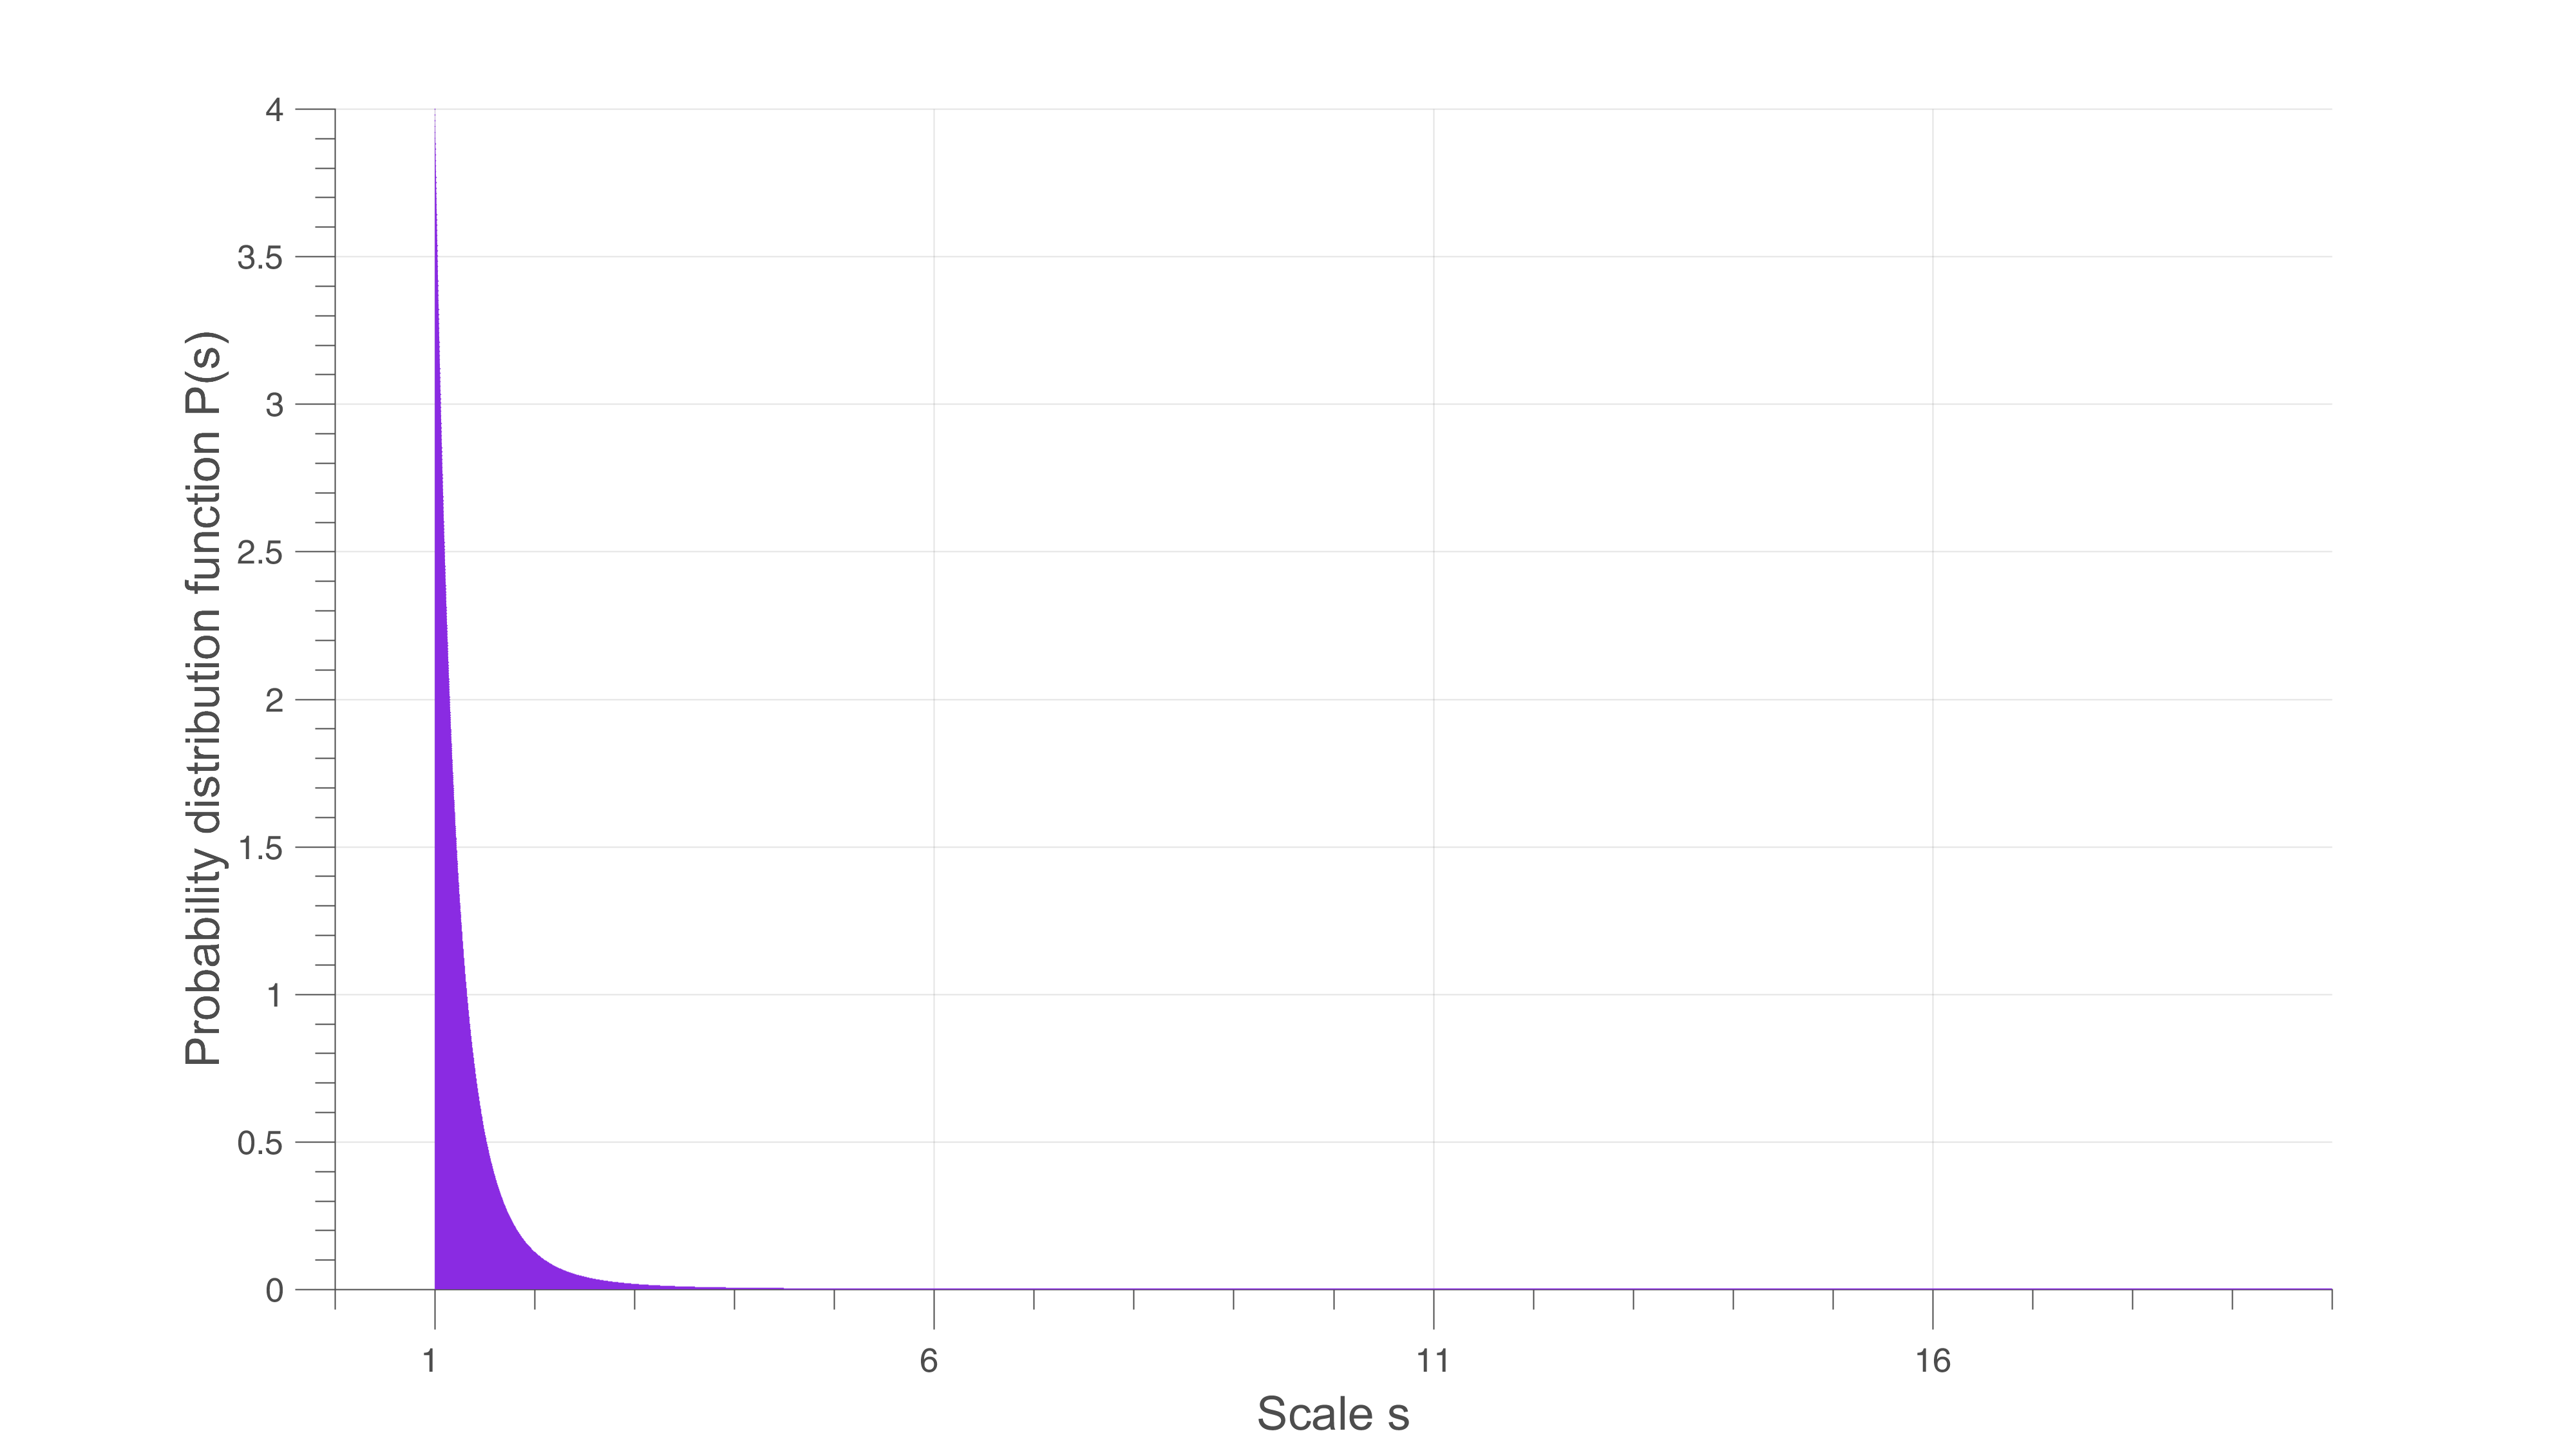
\includegraphics[width=0.9\textwidth]{figures//ps2.png} 
\caption{Weakening scales $s$ probability distribution curve when $\beta=5$ }
\label{ps2}
\end{figure}

\newpage
\subsection{Yield function with mean stress effect}
\label{sec:5.4.3}
Positive mean stress clearly reduces the fatigue life of the material. In design evaluation of multiaxial fatigue with mean stress, a simplified, conservative relation between mean stress and equivalent alternating stress is necessary. We can improve the model to come by modifying the yield function $\sigma_y$ and the localization tensor.

\vspace{6pt}
\textbf{Present choice}
\vspace{6pt}

In the model to come, our idea is to consider as in \cite{Maitournam2011232} that the yield limit $\sigma_y$ can be reduced in presence of positive mean stress. The mesoscopic yield function can therefore be written as:
\begin{equation}
f\left(s\right)=||\uline{\uline{S}}(s)-\uline{\uline{b}}(s)||+\left( \lambda \Sigma_H-\sigma_y\right) /s\leqslant 0
\label{eq.yieldfun}
\end{equation}
with $\uline{\uline{S}}$ denoting the deviatoric part of the stress tensor at microscale, and $\uline{\uline{b}}(s)$ the corresponding backstress at the same scale. The material remain in elastic regime when $f<0$ and in plastic regime when $f=0$. The parameter $\lambda$ can itself be a function of $\Sigma_H$ with a different value in traction($\lambda_+$) than in compression($\lambda_-$).


\subsection{Local plastic model}
We can now describe the mesoscopic stress state.  The model considers a plastic 
behavior at the mesoscopic scale. The mesoscopic stress evolution equations are thus:

\begin{equation}
\dot{\uline{\uline{S}}}(s,M,t)=dev\dot{\uline{\uline{\Sigma}}}(M,t)-\dfrac{E}{1+\nu}\dot{\uline{\uline{\varepsilon}}}^p(s,M,t), 
\label{eq.mesostress}
\end{equation}
which defines a Taylor-Lin scale transition model with unit localization tensor (\cite{Bosia201239}). The mesoscopic deviatoric strain rate tensor is thus equal to the macroscopic strain rate tensor $dev\dot{\uline{\uline{\Sigma}}}=\dfrac{1+\nu}{E}dev\dot{\uline{\uline{\varepsilon}}}$ with $dev\uline{\uline{\Sigma}}$ the deviatoric part of the macroscopic stress tensor. It is complemented by
\begin{equation}
\dot{\uline{\uline{b}}}(s,M,t)=\dfrac{kE}{E-k} \dot{\uline{\uline{\varepsilon}}}^p(s,M,t), 
\label{eq.backstress}
\end{equation}
which is our kinematic hardening model, and by
\begin{equation}
\dot{\uline{\uline{\varepsilon}}}^p(s,M,t)=C\dfrac{\partial f(s,M,t)}{\partial \uline{\uline{S}}}, 
\label{eq.plasticflow}
\end{equation}
which is the associated plastic flow rule assuming $C=0$ when $f<0$ and  $C\geqslant0$ when $f=0$.

Here E denotes the Young's modulus and k the hardening parameter. The local dissipated energy rate per unit volume at weakening scales $s$  is given by the local entropy dissipation:
\begin{equation}
\dot{w}(s,M,t)=(\uuline{S}-\uuline{b})(s,M,t):\uuline{\dot{\varepsilon}}^p(s,M,t).
\label{dissipated}
\end{equation}

\section{Construction of an energy based fatigue approach}
\label{sec:5.5}
In a preliminary step, we will consider a simple macroscopic loading history $\uuline{\Sigma}(M, t)$ which is uniaxial
 along direction $\uline{\uline{s}}_1$, with $\uline{\uline{s}}_1$ a given stress tensor of unit norm. In traction there is 
 $$\uline{\uline{s}}_1=\sqrt{\dfrac{3}{2}}	\left(
 \begin{array}{ccc}
2/3 & 0 & 0\\
 0 & -1/3 & 0\\ 
 0 & 0 & -1/3\\
 \end{array}\right) . $$
  Time periodic of deviatoric amplitude $S_{a}$, constant mean stress $\Sigma_{H}$ and a Von Mises flow rule are taken into account to see if we get a prediction of local failure for a number of cycles $N_F$ varying as $S_{a}^{-\gamma}.$

In uniaxial cyclic loading, there will be 3 kinds of loading patterns, as is shown in \figref{backstress}:

\vspace{6pt}
\begin{enumerate}

\item	Elastic regime, in phase 2 and 4,where we have no plastic flow $\dot{\uline{\uline{\varepsilon}}}^p(s,M,t)=\dot{\uline{\uline{b}}}=0$ ,  and where the stress is below the yield limit $|\uline{\uline{S}}-\uline{\uline{b}}|< \left( \sigma_y-\lambda \Sigma_H\right)/s$, and where we have therefore $\dot{\uline{\uline{S}}}=dev\dot{\uline{\uline{\Sigma}}}$. 
\vspace{6pt}

\item Plastic regime according to plastic flow rule, with increasing plastic deformation, in phase 5 and 1, where	$\dot{\uline{\uline{\varepsilon}}}^p(s,M,t)=\xi\dfrac{\uline{\uline{S}}(s)-\uline{\uline{b}}(s)}{||\uline{\uline{S}}(s)-\uline{\uline{b}}(s)||}> 0$ with  $\xi= \left| dev\dot{\uline{\uline{\Sigma}}}\right| \left(\dfrac{kE}{E-k}+\dfrac{E}{1+\nu} \right) ^{-1}$(detailed in annex) ,  $\uline{\uline{S}}-\uline{\uline{b}}=\uline{\uline{s}}_1 \left(\sigma_y-\lambda \Sigma_H\right)/s$ and $\dot{\uline{\uline{S}}}-\dot{\uline{\uline{b}}}=0.$ 
\vspace{6pt}

\item Plastic regime in the other direction, in phase 3, where we now have	$\dot{\uline{\uline{\varepsilon}}}^p(s,M,t)<0$,  then $\uline{\uline{S}}-\uline{\uline{b}}=-\uline{\uline{s}}_1 \left(\sigma_y-\lambda \Sigma_H\right)/s$ and $\dot{\uline{\uline{S}}}-\dot{\uline{\uline{b}}}=0$.

\end{enumerate}	

\begin{figure}[!h]
\centering
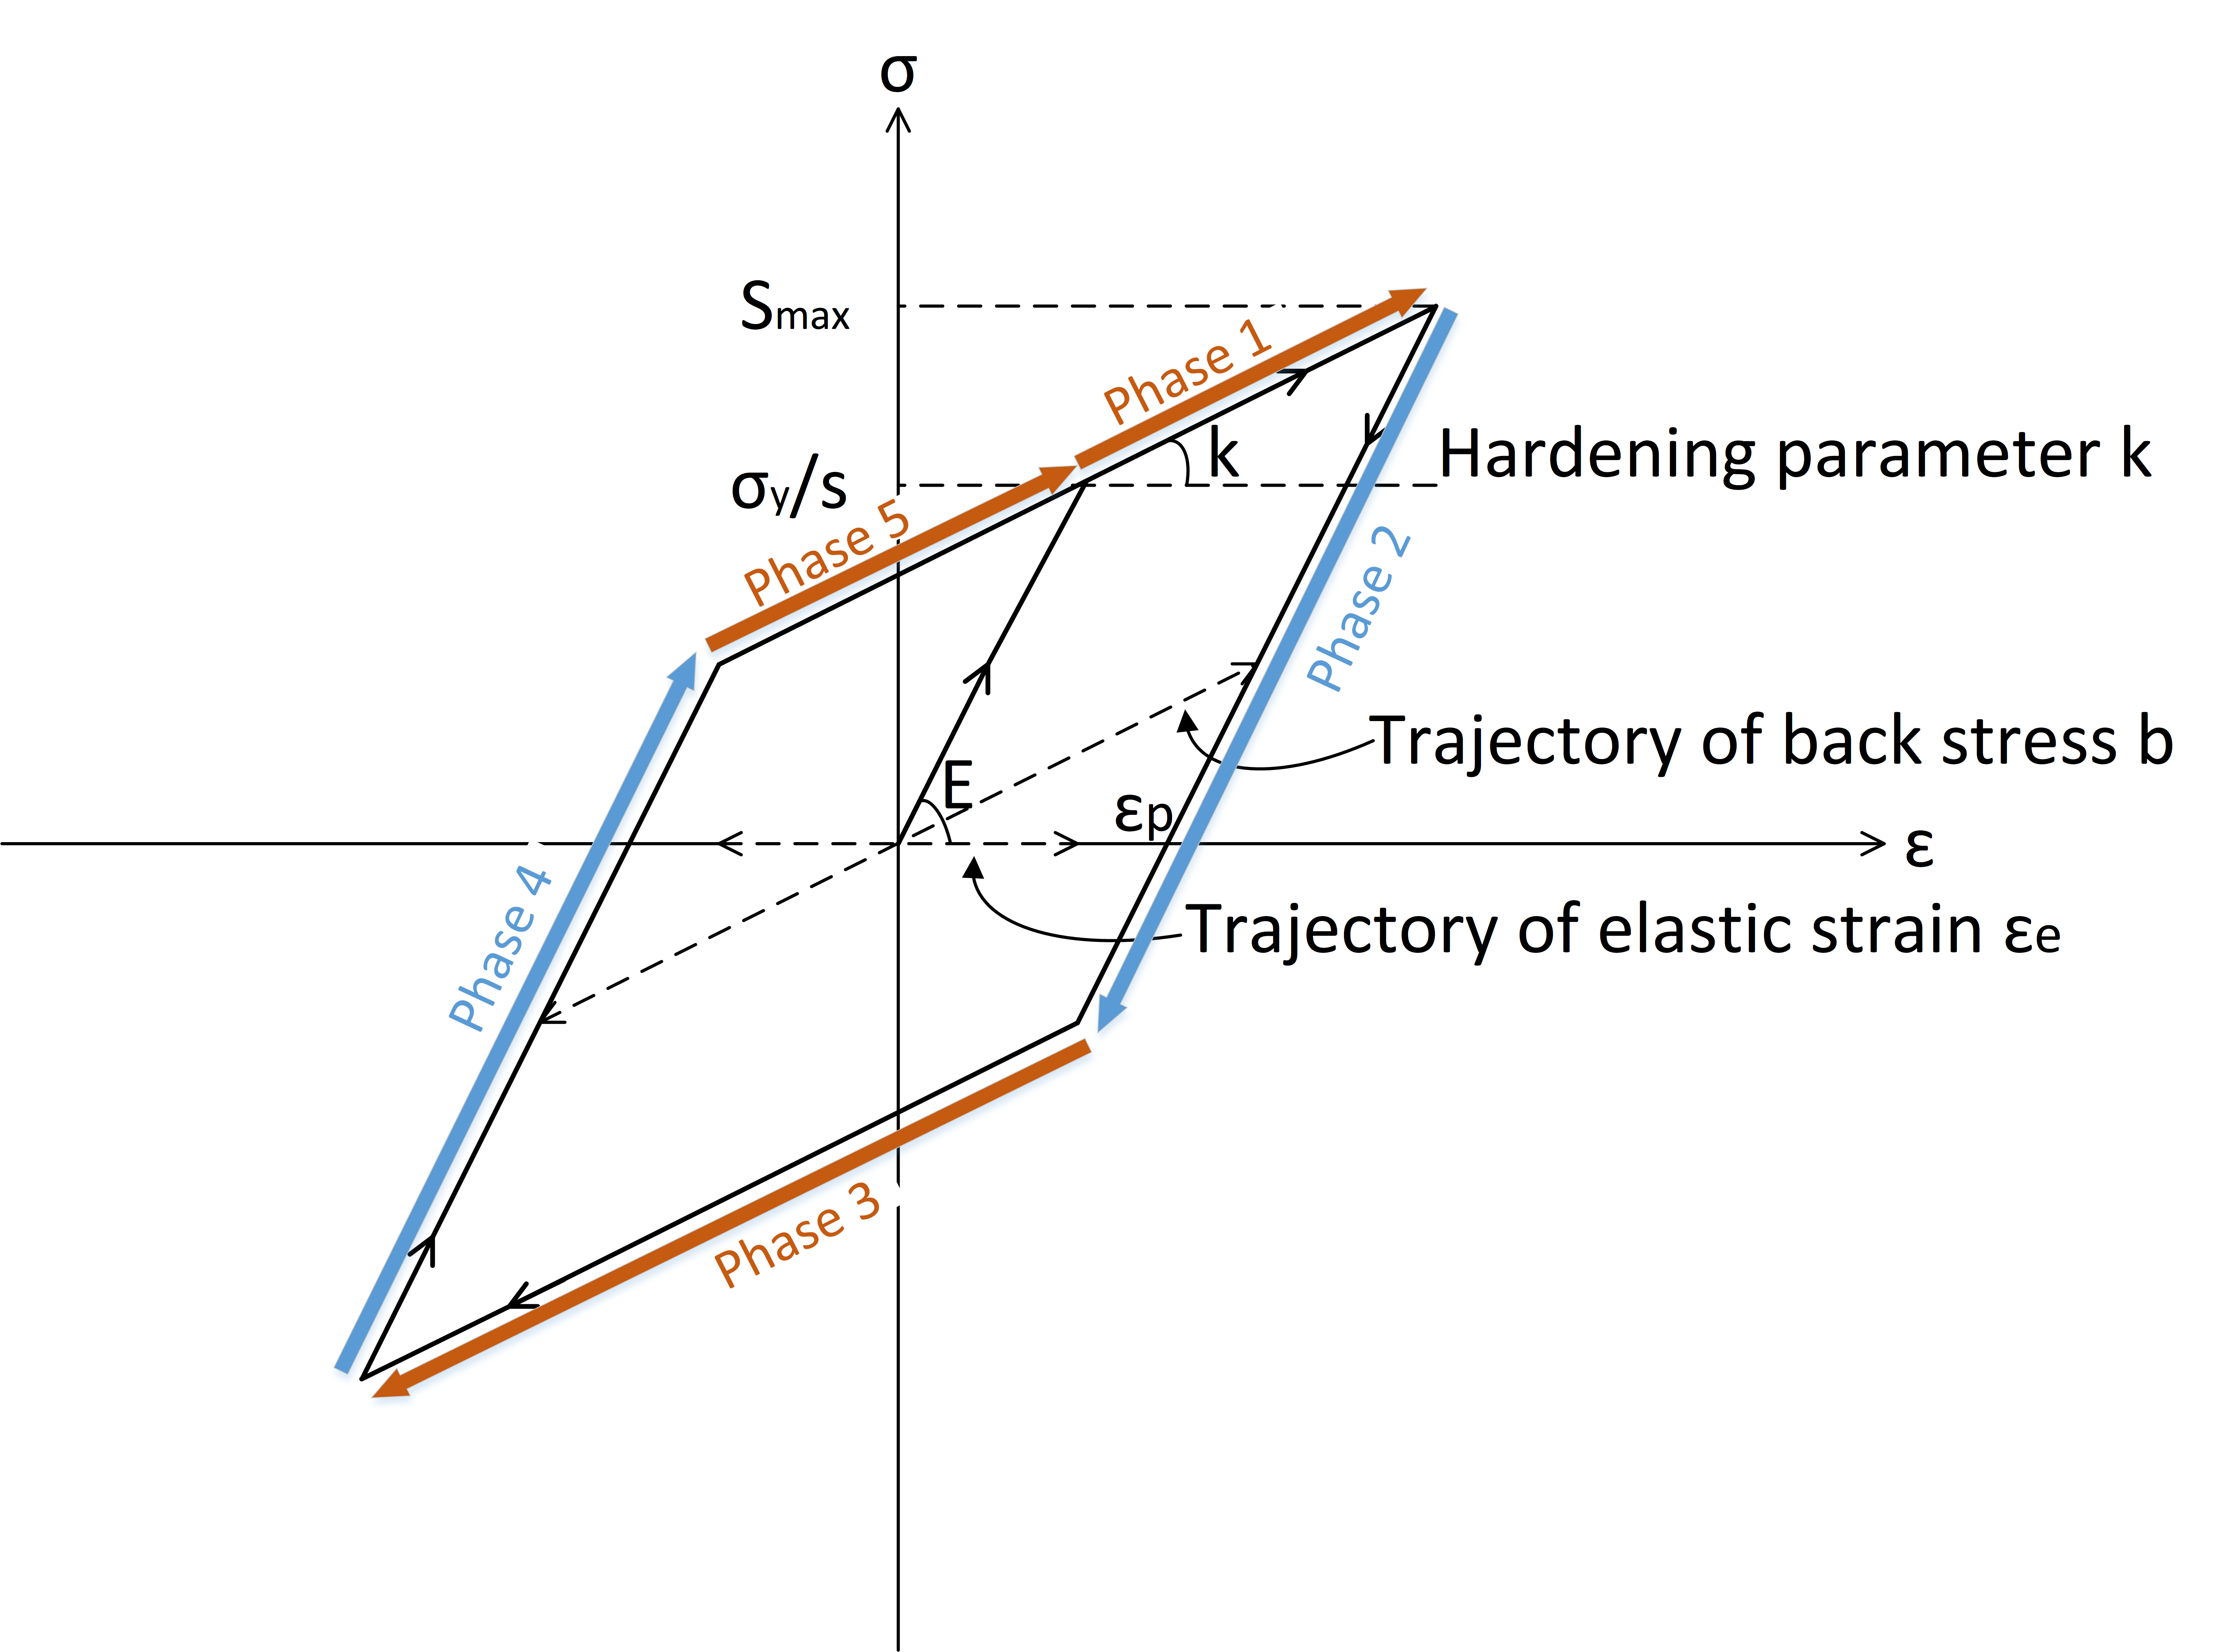
\includegraphics[width=0.9\textwidth]{figures//backstress.png} 
\caption{Uniaxial load with plastic dissipation}
\label{backstress}
\end{figure}

In phase 1, a direct analysis yields the energy dissipation at scale $s$:
\begin{equation}dW=(S-b)d\varepsilon^p=\dfrac{(E-k)(1+\nu) }{E(E+k\nu)}\dfrac{ \left(\sigma_y-\lambda \Sigma_H\right)}{s}\left(S_{a}-\dfrac{ \left(\sigma_y-\lambda \Sigma_H\right)}{s}\right).
\label{dw}
\end{equation}

A similar analysis yields $$dW(phase 1)=dW(phase 5)=\dfrac{1}{2}dW(phase 3).$$

We can then calculate  the local dissipated energy $W$  at point $M$ during one cycle by cumulating the input of all sub-scales plastic regime with their probabilities (\cite{zepeng}).
\begin{equation}
\begin{split}
W_{cyc}&=4\int_{ \left(\sigma_y-\lambda \Sigma_H\right) /S_{a}}^{\infty}dW(s,M,t)P(s)ds
\\&=4\int_{ \left(\sigma_y-\lambda \Sigma_H\right) /S_{a}}^{\infty}\dfrac{(E-k)(1+\nu) }{E(E+k\nu)}\dfrac{ \left(\sigma_y-\lambda \Sigma_H\right)}{s}\left(S_{a}-\dfrac{ \left(\sigma_y-\lambda \Sigma_H\right)}{s}\right)\left( \beta-1\right) s^{-\beta}ds
\\&=\dfrac{4(E-k)(1+\nu)\left( \beta-1\right) }{ E(E+k\nu)\beta\left( \beta+1\right) }\dfrac{S_{a}^{\beta+1}}{ \left(\sigma_y-\lambda \Sigma_H\right)^{\beta-1}}.
\end{split}
\label{eq:w}
\end{equation}

So we have a power law relationship between stress intensity and the dissipated energy per cycle.
\begin{equation}
W_{cyc}=C_1S_{a}^{\beta+1},
\label{eq.wcyc}
\end{equation}
with 
$$C_1=f(\lambda,\beta)=\dfrac{4(E-k)(1+\nu)\left( \beta-1\right) }{ E(E+k\nu)\beta\left( \beta+1\right)\left(\sigma_y-\lambda \Sigma_H\right)^{\beta-1} }.$$
If the dissipated energy accumulates until a failure value $W_0$, we can get directly the number of cycles to failure from Eq.\eqref{eq.wcyc} as:
\begin{equation}
N_{F}=\dfrac{W_0}{W_{cyc}}=\dfrac{W_0}{C_1}S_{a}^{-\beta-1}.
\label{eq.NFcyc}
\end{equation}
As for the time to failure in cyclic loading, it will be:
$$T_{F}=N_{F}t_{cyc}.$$
From Eq.\eqref{eq:w}, we then obtain that in uniaxial cyclic loading the model predicts as expected (Chapter \ref{chp:4}) a power law dependence of the number of cycles to failure in function of $S_{a}$.
However, experiments shows that the damage or the energy accumulation of a material evolves non-linearly in time and present a load dependent cycle (Chapter \ref{chp:4}). We should introduce below a method to handle such a nonlinearity.

\section{Nonlinearity of damage accumulation}
\label{sec:5.6}
\subsection{Energy approach with Chaboche law}
The Chaboche law (\cite{lemaitre1990mechanics}) is essentially a damage incremental law for cyclic loads with a deviatoric stress intensity ${A}_{\uppercase\expandafter{\romannumeral2}}$ and hydrostatic mean part $\Sigma_H$, defining the damage increase by:

\begin{equation}\delta D = \left( 1 -(1-D)^{\gamma+1}\right)^\alpha \left(\frac{{A}_{\uppercase\expandafter{\romannumeral2}} }{M(\sigma_H)\left( 1-D\right)}\right)^\gamma \delta N ,
\label{chabochemulti}
\end{equation} 

using an effective intensity ${A}_{\uppercase\expandafter{\romannumeral2}}^*={A}_{\uppercase\expandafter{\romannumeral2}}/\left( 1-D\right) $ evolving with damage $D$. And the mean stress effect is present both in exponential factor $\alpha$ and in denominator $M(\sigma_H)$.
$$\alpha=1 - a\left\langle \dfrac{\dfrac{1}{2}{A}_{\uppercase\expandafter{\romannumeral2}}-\sigma_{-1}M(\sigma_H) }{\sigma_{u} -{A}_{\uppercase\expandafter{\romannumeral2}}}\right\rangle,$$
$$M(\sigma_H) =M_0 \left(1-3c\sigma_{H,max}\right).$$

Eq.\eqref{chabochemulti} writes equivalently:
\begin{equation}\delta [1-(1-D)^{\gamma+1}]^{1-\alpha}=(1-\alpha)(\gamma+1)\left(\dfrac{{A}_{\uppercase\expandafter{\romannumeral2}} }{M(\Sigma_H)}\right)^\gamma \delta N=\dfrac{1}{N_F(\sigma)}\delta N.
\label{integration}
\end{equation}
Here $N_F(\sigma)$ denotes the number of cycles at intensity $\sigma$ to failure as obtained by integration of Eq.\eqref{integration} from $D=0$ to $D=1$. 

%
%The nonlinear damage incremental law using energy dissipation:
%\begin{equation}
%\begin{split}
%  \delta D &=\dfrac{\left( 1 -(1-D)^{\gamma+1}\right)^\alpha}{\left(1-D \right)^\gamma} \delta W
%  \\&= \dfrac{\left( 1 -(1-D)^{\gamma+1}\right)^\alpha}{\left(1-D \right)^\gamma} \dfrac{W_{cyc}\delta N}{W_0}
%  \\&= \dfrac{\left( 1 -(1-D)^{\gamma+1}\right)^\alpha}{\left(1-D \right)^\gamma} \dfrac{4(E-k)(1+\nu)\left( \beta-1\right) }{ E(E+k\nu)\beta\left( \beta+1\right) }\dfrac{S_{a}^{\beta+1}}{\left(\sigma_y-\lambda \Sigma_H\right)^{\beta-1}}\dfrac{\delta N}{W_0}.
%\end{split}
%\label{recoverchaboche}
%\end{equation} 
%
%We compare Eq.\eqref{chabochemulti} and Eq.\eqref{recoverchaboche}, in Chaboche model there is:
%$$\beta+1=\gamma. $$

Similar to Eq.\eqref{integration}, we define here the ``equivalent damage'' $\tilde{D}$(\figref{eq.Dhat}) :

\begin{equation}
\tilde{D}=1-(1-D)^{\gamma+1},
\label{eq.Dhat}
\end{equation}
with $D$ the damage variable introduced by Chaboche in its model to scale the stress intensity:
$${A}_{\uppercase\expandafter{\romannumeral2}} \longrightarrow \dfrac{{A}_{\uppercase\expandafter{\romannumeral2}}}{1-D}.$$

We have 

$\bullet$ $\tilde{D}=0$ when $D=0$ (undamaged material),

$\bullet$ $\tilde{D}=1$ when $D=1$ (failure of material),	

and a nonlinear relation in between as in \figref{fig.Dhat}:
$$\delta\tilde{D}=\left(\gamma+1 \right)\left( 1-D\right)^\gamma \delta D.$$	
\begin{figure}
\centering
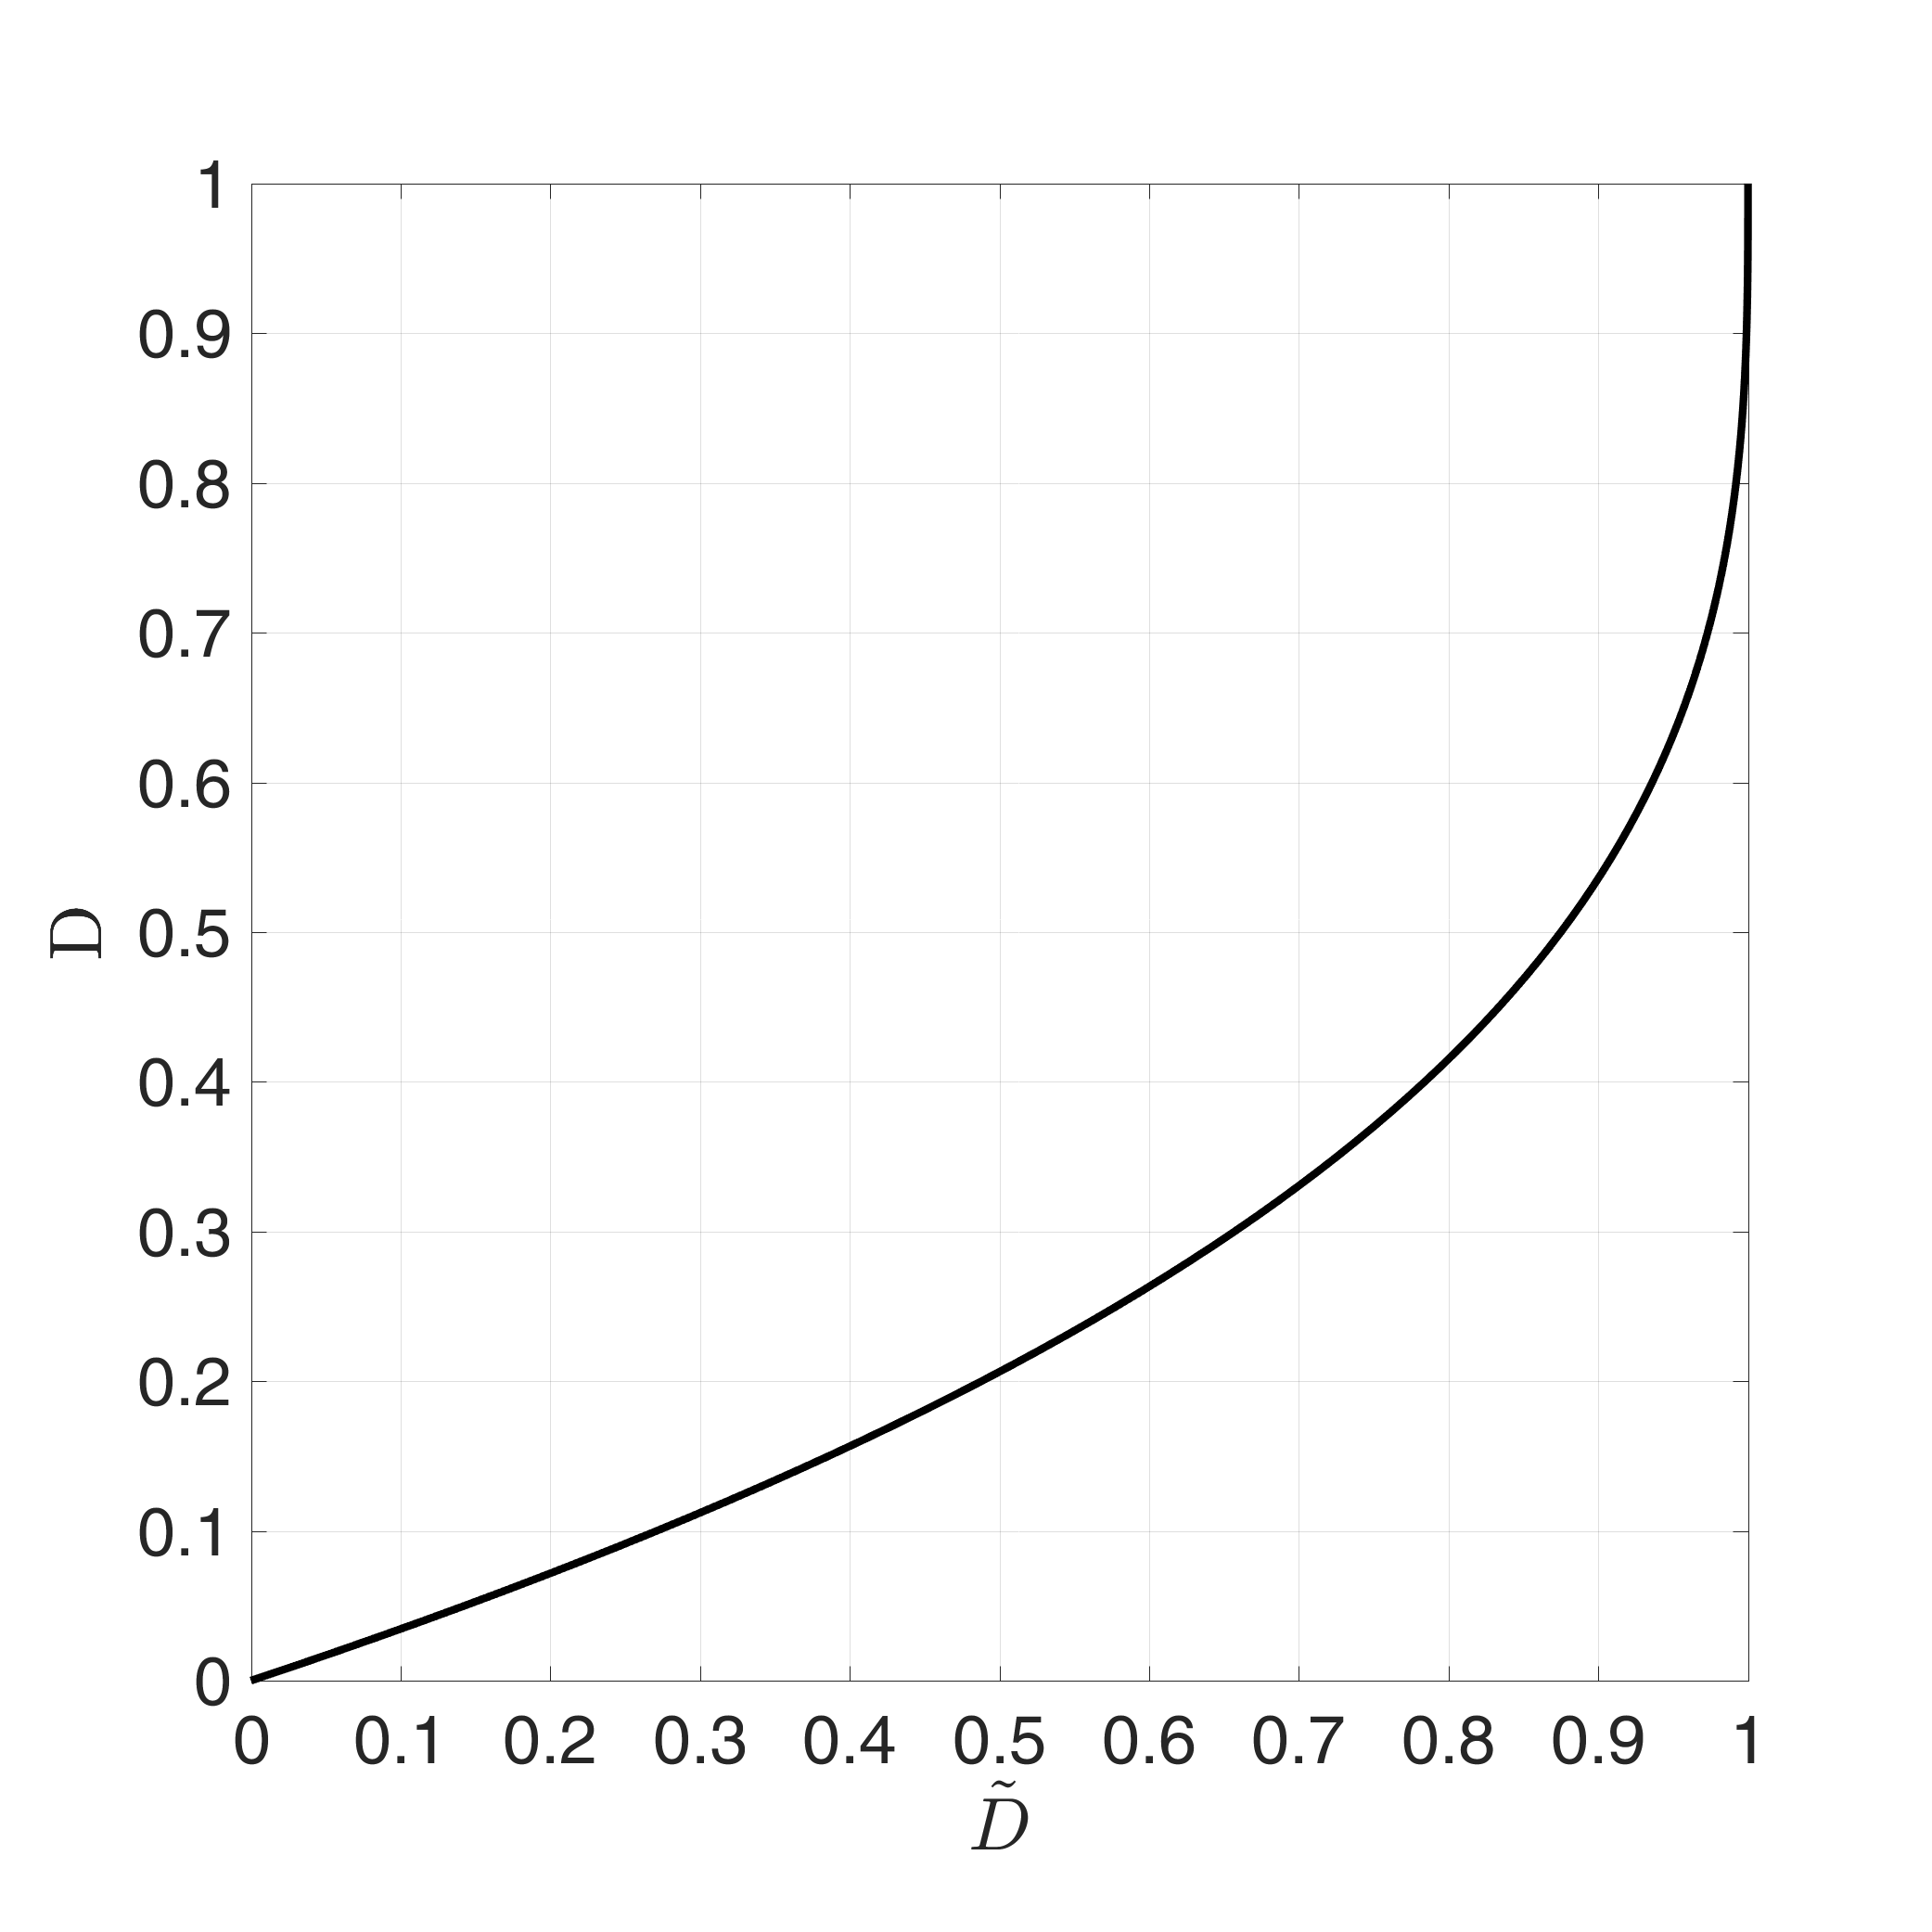
\includegraphics[width=0.6\textwidth]{figures//Dhat.png} 
\caption{The relation between $\tilde{D}$ and $D$ when $\gamma=2$}
\label{fig.Dhat}
\end{figure}

Change of damage measure $\tilde{D} = 1 - (1-D)^{\gamma+1}$ makes the evolution \eqref{chabochemulti} explicit. It writes
\begin{equation}
\dfrac{d\tilde{D}}{dN} = c_D {\tilde{D}}^\alpha \left(\dfrac{{A}_{\uppercase\expandafter{\romannumeral2}}}{M(\Sigma_{H})} \right) ^\gamma,
\label{eq.diffchaboche}
\end{equation}
yielding after integration from $\tilde{D}=0$ to $\tilde{D}=1$  a number of cycles to fatigue at constant load given by
$$
N_F =\dfrac{1}{(1-\alpha)}\left(\dfrac{{A}_{\uppercase\expandafter{\romannumeral2}}}{M(\Sigma_{H})} \right) ^{-\gamma}.
$$

This method as written requires cycle counting which is difficult and technical for complex load histories. In addition, it allows only a limited influence of multiaxiality.


Now in our model we use the same growth rule as in Chaboche in cyclic load regime, but replace stress intensity by multiscale dissipated energy  in Eq.\eqref{eq.diffchaboche}, which removes cycle counting.

The evolution \eqref{eq.diffchaboche} then writes
$$
\dfrac{d\tilde{D}}{dt} ={\tilde{D}}^\alpha \dot{W}/W_0,
$$
or in a differential form
\begin{equation}
d \tilde{D}=\tilde{D}^\alpha\dfrac{d W}{W_0}=\tilde{D}^\alpha\dfrac{W_{cyc}d N}{W_0}.
\label{eq.DWcyc}
\end{equation}

The replacement of $d W$ by $W_{cyc}dN$ is only introduced to handle cyclic loadings if they occur. The number of cycles to failure in constant loading case, obtained by integrating $\tilde{D}$ from $\tilde{D}_0$ to 1 is then:
$$N_F=\dfrac{W_0}{\left( 1-\alpha\right)W_{cyc} }\left( 1-D_0^{1-\alpha}\right) .$$
With initial damage $D_0=0$, we finally get with our proposed expression Eq.\eqref{eq.wcyc} of cyclic energy dissipation:
\begin{equation}
N_F=\dfrac{W_0}{\left( 1-\alpha\right)W_{cyc} }=\dfrac{W_0}{(1-\alpha)C_1}S_{a}^{-\beta-1}.
\label{eq.NFWcyc}
\end{equation}

From Eq.\eqref{eq.NFWcyc}, we see $(-\beta-1)=-\gamma$ is related to the slops in S-N curve and that $\dfrac{W_0}{(1-\alpha)C_1}$ defines the number of cycles to failure.
\subsection{Sequence effect}

Experiments show fatigue tests started with high stress then change to low stress has less fatigue life than the combination of high stress life proportion plus the low one. This phenomenon of sequence effect is load history dependent, so we need a stress induced parameter to describe it. 

This is done in Chaboche  with three ingredients:

\begin{enumerate} 
\vspace{6pt}
\item a damage sensitive effective stress: 
$$\sigma_D^{eff} = J_2(\uline{\uline{\Sigma}})/(1-D)={A}_{\uppercase\expandafter{\romannumeral2}}/(1-D);$$

\vspace{6pt}

\item a $(\sigma_D^{eff})^\gamma$ controlled  law for damage growth
$$\dfrac{dD}{dN} =c_\gamma {\tilde{D}}^\alpha (\sigma_D^{eff})^\gamma;$$

\vspace{6pt}

\item  a load dependence of exponent $\alpha$ (from $1$ at zero load to $0$ at large loads). In Chaboche model, the proposition of $\alpha$ is
\begin{equation}
\alpha = 1 - a\left\langle \frac{ \sigma_{eq}-\sigma_{fatigue}}{ \sigma_{u} - \sigma_{eq}}\right\rangle
\label{eq.alpchaboche}
\end{equation}
in order to recover the proper high-low sequencing effect.
\end{enumerate}

Many fatigue damage accumulation models are based on the two level loading experiments which is one of the basic random loading analysis. To facilitate the validation and interpretation of an $\alpha$ dependence on stress we will also use two-stress level loading, the specimen is firstly loaded at stress $\Sigma_1$ for $T_1$ cycles and then at stress $\Sigma_2$ for $T_2$ cycles until failure. We can then observe if the experimental results are satisfactory.

During a loading time $T_1$, we  cycle  from $\tilde{D}=0$ to $\tilde{D}= \tilde{D}_1$. By integrating Eq.\eqref{eq.DWcyc} of our proposed approach, we get:
\begin{equation}
\left( 1-\tilde{D}_1\right) ^{1-\alpha_1}=\dfrac{T_1}{T_{F1}},
\label{23a}
\end{equation}
with $T_{F1}$ the time to failure with this loading.

Then we cycle from  ${\tilde D}={\tilde D}_1$ to failure ${\tilde D}=1$, which yields
\begin{equation}
1-\left( 1-\tilde{D}_1\right)^{1-\alpha_2}=\dfrac{T_2}{T_{F2}}.
\label{23b}
\end{equation}

From Eq.\eqref{23a} and Eq.\eqref{23b}, after elimination of $\left( 1-D_1\right)$ we get:
\begin{equation} 
\dfrac{T_2}{T_{F2}} =1-\left( \dfrac{T_1}{T_{F1}}\right) ^\eta,
\label{eq.sequence}
\end{equation}
with
\begin{equation}
\eta=\dfrac{1-\alpha_2}{1-\alpha_1}.
\label{eq.eta}
\end{equation}

In the case of high-low loading sequence we have $\Sigma_1>\Sigma_2$,  which gives $\alpha_1<\alpha_2$, so it comes to:
$$\eta=\frac{1-\alpha_2}{1-\alpha_1}<1 \implies
\frac{T_2}{T_{F2}}=1-\left( \frac{T_1}{T_{F1}}\right) ^\eta<1-\frac{T_1}{T_{F1}} \implies
\frac{T_1}{T_{F1}}+\frac{T_2}{T_{F2}}<1.$$

The $\alpha$ dependence on stress intensity does therefore predict a sequencing effect where a low loading sequence following a high one will reduce the life of the structure if $\alpha$ decreases when the load increases.

To get the same effect in our construction, we propose here to introduce $s_{min}$, which is the minimum scale that experiences plastic dissipation thus causes energy loss:
\begin{equation}
s_{min}=\dfrac{\left(\sigma_y-\lambda \Sigma_H\right)}{S_{a}}.
\label{eq.smin}
\end{equation}

We propose a load dependent $\alpha$ through $s_{min}$. Possible choice
of $\alpha$ is expressed as Eq.\eqref{eq.alpha}:
\begin{equation}
\alpha=1-a\left( \dfrac{\frac{1}{s_{min}}}{1-\frac{1}{s_{min}}} \right) .
\label{eq.alpha}
\end{equation}

There is no notion of fatigue limit in our model, $\sigma_{faigue}=0$. The intensity of loading
$$\frac{ \sigma_{eq}-\sigma_{fatigue}}{ \sigma_{u} - \sigma_{eq}}= \frac{ 1}{\frac{\sigma_{u}}{\sigma_{eq}} -1}$$
is measured by 
$$\left( \dfrac{\frac{1}{s_{min}}}{1-\frac{1}{s_{min}}}\right) =\left(s_{min}-1 \right) ^{-1}.$$
This means that we measure the distance of load to ultimate failure by local variable $s_{min}$ through 

$$\frac{\sigma_{u}}{\sigma_{eq}} -1 \longrightarrow \left( s_{min}-1\right)  $$


We can see from \figref{fig.sequence} that with our proposition, cycling $1$ for fifty percent of its failure time leaves a reserve before failure to cycling $2$ of much less than fifty percent. To conclude, the cumulative damage under high-low loading sequence, as we deduced, has the addition of partial lives less than unit. Similarly, the cumulative damage under low-high loading sequence has addition of partial lives more than 1:
$$\frac{T_1}{T_{F1}}+\frac{T_2}{T_{F2}}>1.$$
The curve in both cases is depicted in \figref{fig.sequence}.
\begin{figure}[!h]
\centering
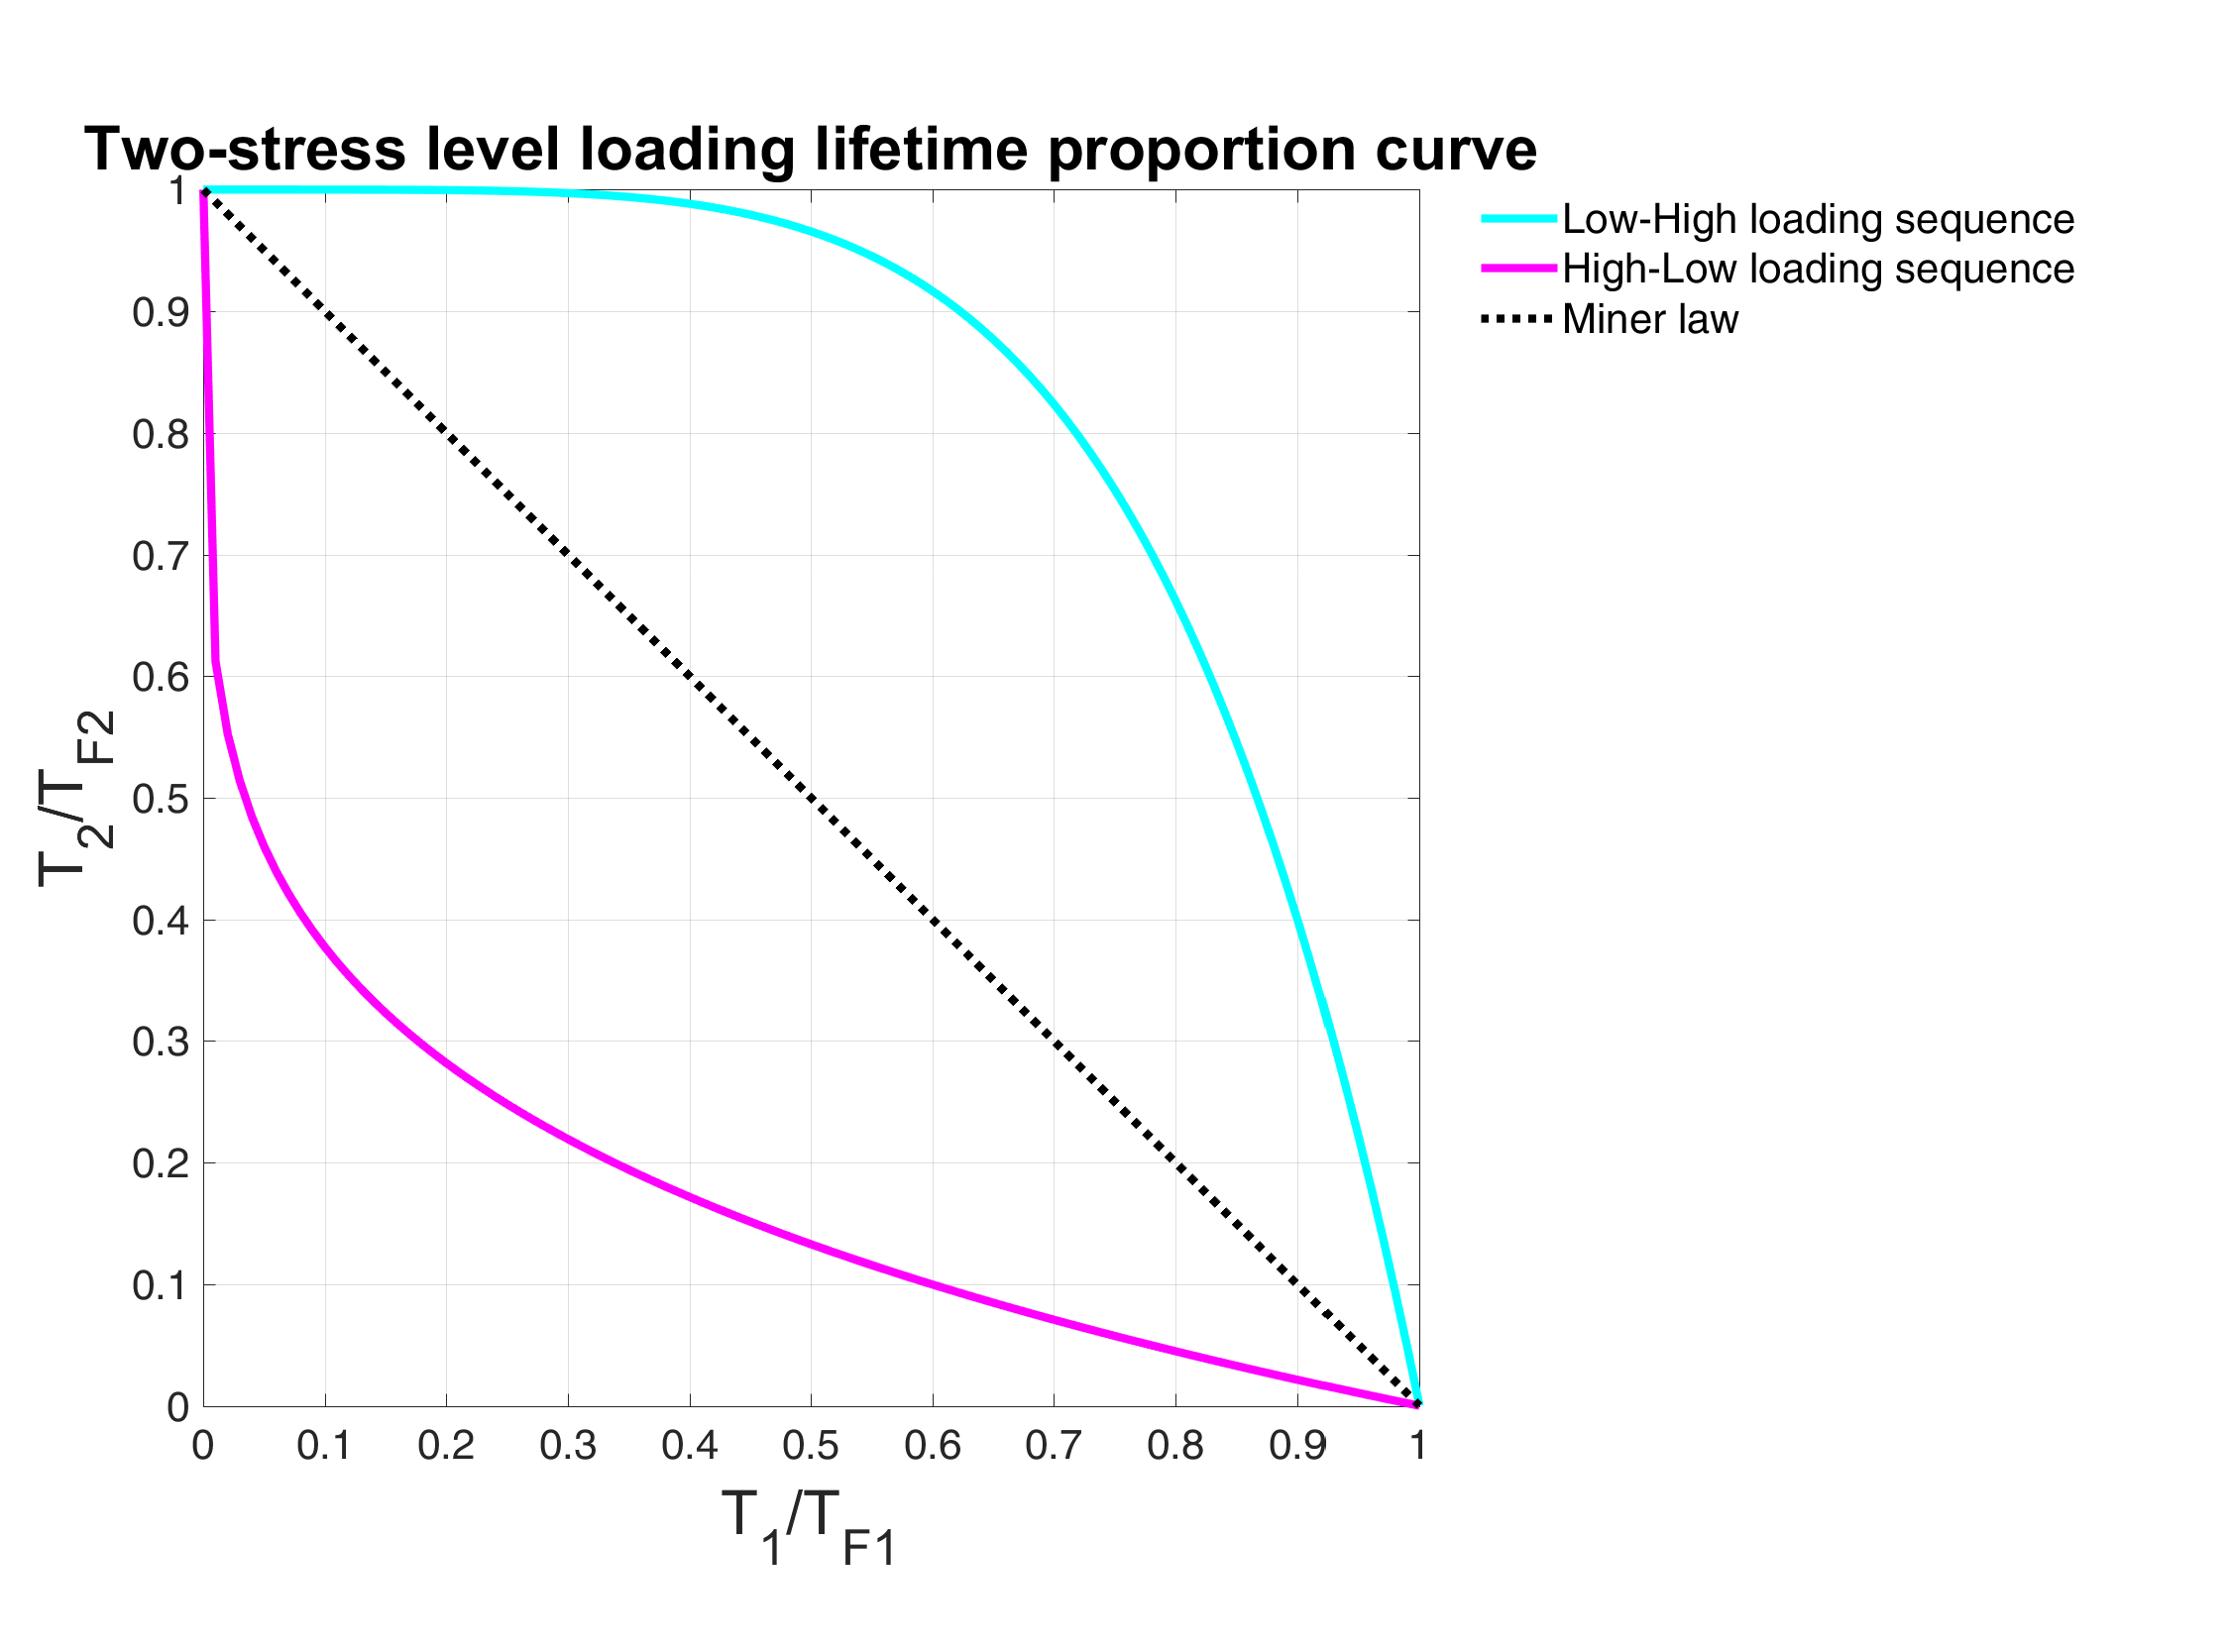
\includegraphics[width=0.8\textwidth]{figures//sequence.png} 
\caption{High to low and low to high loading sequence comparison in 4-point bending($F_{low}=5000 N, F_{high}=30000 N, Radius=0.2m, \Sigma_u=1.67E8$), with the proposed damage accumulation law (Eq.\eqref{eq.DWcyc}) induced equation Eq.\eqref{eq.sequence} and Chaboche type $\alpha$ (Eq.\eqref{eq.alpchaboche}) containing Crossland criterion}
\label{fig.sequence}
\end{figure}
For constant two-level stress loading, $\alpha_1=\alpha_2$, the Chaboche law returns to the Miner rule when $F_{low}=F_{high}$ where:
$$\frac{T_1}{T_{F1}}+\frac{T_2}{T_{F2}}=1.$$

\newpage
\subsection{The final model}
\label{sec:5.6.3}
In summary, our damage based fatigue life criterion using a damage evolution governed by a multiscale plastic energy dissipation, has four ingredients.
\begin{itemize}
\item  a scale dependent yield limit $$\frac{1}{s} (\sigma_y- \lambda \Sigma_H^{macro})$$ associated to a microscopic plastic evolution governed by the standard plastic evolution laws Eq.\eqref{eq.mesostress} - Eq.\eqref{eq.plasticflow};

\vspace{6pt}	

\item a multiscale plastic energy dissipation obtained by summing plastic dissipation across our power law scale distribution
\begin{equation}
\dot{W}(M,t)=\int_{s=1}^{\infty}\left(\uline{\uline{S}}-\uline{\uline{b}} \right) (s,M,t):\uline{\uline{\dot{\varepsilon}}}^p(s,M,t) s^{-\beta}ds;
\label{eq.final2}
\end{equation}

\vspace{6pt}	

\item a load intensity sequencing effect that we have represented by the formula : 
\begin{equation}
1 - \alpha = a (s_{min}-1)^{-f};
\label{eq.final3}
\end{equation}

\vspace{6pt}	

\item a exponential damage evolution law with load dependent exponent $\alpha$ given by the above formula and coefficient $\dot{W}/W_0$ governed by the multiscale plastic dissipation rate: 
\begin{equation}
\dfrac{d\tilde{D}}{dt} ={\tilde{D}}^\alpha \dot{W}/W_0.
\label{eq.final4}
\end{equation}
\end{itemize}

In this model we have five independent coefficients in addition to the construction of the local plastic model Eq.\eqref{eq.mesostress} - Eq.\eqref{eq.plasticflow} :

\begin{enumerate}
\item reference density of damage energy : $W_0$ (in MPa)

\item mean stress effect coefficient : $\lambda$
\item slope of SN curve : $\beta+1$

\item sensitivity to load intensity $a$. 
\item exponent in the load sequence effect $f$. 
\end{enumerate}

\newpage
\section{Numerical strategy}
\label{sec:5.7}
\subsection{Scale discretization}
We now need to propose a practical implementation strategy for our final model of section \ref{sec:5.6.3}.Our first approach takes one cycle as unit time. We compute analytically by Eq.\eqref{eq:w} the energy dissipation at each scale during this cycle. The method is valid for simple loading history and which includes the integration on all weakening scales. The damage $\tilde{D}$ is then accumulated after each cycle by numerical integration of Eq.\eqref{eq.final4} until we get to the fatigue limit of $\tilde{D}=1$.

However, there are certain limitations of this method. Firstly we need a load history decomposition in cycles. Secondly in real life the perfect close loop cycle is hardly applicable. Finally, we need to approximate $\alpha$  by its average value per cycle which is computed numerically and can not be done analytically.

Thus we propose in a more general method which can be integrated by a step by step strategy. We compute numerically the dissipation at different scales using an implicit Euler time integration of the constitutive laws of section \ref{sec:5.4.4}. After which we make a numerical integration on different scales. Then we can update the damage and go to next time step. 

Instead of doing the scale integration directly which can be difficult for complex loading, the Gaussian Quadrature rule with Legendre points is used to give the value of local dissipated energy rate. To use the Gaussian quadrature rule the limit range of integral must be from $-1$ to $1$, while the total dissipated energy  is expressed by integrating all the weakening scale $s$ ranging from 1 to infinity with their occurrence probabilities:
$$\dot{W}=\int_{1}^{\infty}\dot{w}(s) (\beta-1)(s)^{-\beta}ds.$$

\noindent
To change the limit range of integral from $[1,\infty]$ to $[1,0]$ we take as new integration variable
$u(s)= s^{1-\beta}$. Therefore the dissipated energy summed on all scales is:
\begin{equation}
\begin{split}
\dot{W}&=\int_{1}^{\infty}\dot{w}(s) (\beta-1)(s)^{-\beta}ds
\\&=\int_{0}^{1}\dot{w}\left( u^{\frac{1}{1-\beta}}\right)du
\\&=\frac{1}{2}\int_{-1}^{1}\dot{w}\left[  \left( \frac{x+1}{2}\right) ^{\frac{1}{1-\beta}}\right] dx
\end{split}
\label{allscale}
\end{equation}
given $u=\dfrac{x+1}{2}$. So the dissipated energy rate integrated over all scales takes the form of Eq.\eqref{allscalerate}:
\begin{equation}
\dot{W}=\frac{1}{2}\int_{-1}^{1}\dot{w}\left[  \left( \frac{x+1}{2}\right) ^{\frac{1}{1-\beta}},t\right] dx\approx\frac{1}{2}\sum_{i}\omega_i\dot{w}\left[  \left( \frac{x_i+1}{2}\right) ^{\frac{1}{1-\beta}},t\right],
\label{allscalerate}
\end{equation}
where $\omega_i$ and $x_i$ are respectively the weights and nodes of the Gauss Legendre integration rule used for the numerical integration.  In this work, we used a 64 points Gaussian Legendre integration rule (\cite{Legendre}) with $s_i=\left( \dfrac{x_i+1}{2}\right) ^{\frac{1}{1-\beta}}$ being the associated scale.

\subsection{Calculation of local plastic dissipation}
\label{sec:5.4.4}
The material could be both in elastic and plastic regime depending on the considered scale. To be more elaborate, we reuse the fundamental equations in different regimes. At scale $s$, we have a dissipation rate given by:
$$\dot{w}(s)=\left( \uline{\uline{S}}-\uline{\uline{b}}\right):\dot{\uline{\uline{\varepsilon}}}^p, $$
which differs between plastic and elastic regime.

\vspace{6pt}
\noindent
\textbf{Elastic regime:}

\vspace{6pt}
\noindent
There we have
plastic strain rate
$\dot{\uline{\uline{\varepsilon}}}^p=0$, back stress rate $\dot{\uline{\uline{b}}}=0$ and deviatoric stress rate $\dot{\uline{\uline{S}}}=dev\dot{\uline{\uline{\Sigma}}}$, leading to
$$\dot{\uline{\uline{S}}}-\dot{\uline{\uline{b}}}=dev\dot{\uline{\uline{\Sigma}}},$$ 
meaning
$$\left( \uline{\uline{S}}-\uline{\uline{b}}\right) (t+dt)=\left( \uline{\uline{S}}-\uline{\uline{b}}\right) (t)+dev\dot{\uline{\uline{\Sigma}}}dt.$$
At each time step we define a trial stress:
\begin{equation}
\left( \uline{\uline{S}}-\uline{\uline{b}}\right)_{trial}:=\left( \uline{\uline{S}}-\uline{\uline{b}}\right)(t+dt).
\label{trial}
\end{equation}
We are in elastic regime at scale $s$ as long as we satisfy

\begin{equation}
\left| \left|  \uline{\uline{S}}-\uline{\uline{b}}\right| \right| _{trial}\leqslant\left( \sigma_y-\lambda \Sigma_H\right)/s.
\label{eq.trialelastic}
\end{equation}

\vspace{6pt}
\noindent
\textbf{Plastic regime:}
\vspace{6pt}

\noindent
When we leave elastic regime at scale s, i.e. when the above inequality Eq.\eqref{eq.trialelastic} is violated, we have:
\begin{numcases}{}
\dot{\uline{\uline{\varepsilon}}}^p=\xi\dfrac{\uline{\uline{S}}-\uline{\uline{b}}}{\left| \left|\uline{\uline{S}}-\uline{\uline{b}}\right| \right|}, \xi>0, & plastic   flow, \label{plasticflow}
\\
\left| \left|\uline{\uline{S}}-\uline{\uline{b}}\right| \right|= \left(\sigma_y-\lambda \Sigma_H\right)/s, & yield   limit,\label{yieldlimit}
\\
\left( \uline{\uline{S}}-\uline{\uline{b}}\right) :\left( \dot{\uline{\uline{S}}}-\dot{\uline{\uline{b}}}\right) =0, & yield   limit   time invariance,
\\
\dot{\uline{\uline{b}}}=\dfrac{kE}{E-k}\dot{\uline{\uline{\varepsilon}}}^p, & kinematic   hardening  rule, \label{kinematichardening}
\\
\dot{\uline{\uline{S}}}=dev\dot{\uline{\uline{\Sigma}}}-\dfrac{E}{1+\nu} \dot{\uline{\uline{\varepsilon}}}^p, & localisation  rule. \label{localisation}
\end{numcases}

In all cases, we get by integrating Eq.\ref{localisation}, Eq.\ref{kinematichardening} with the use of Eq.\ref{plasticflow}.
\begin{equation}
\left( \uline{\uline{S}}-\uline{\uline{b}}\right) (s,t+dt)=\dfrac{\left( \uline{\uline{S}}-\uline{\uline{b}}\right)_{trial} (s,t+dt)}{1+\eta},
\end{equation}

and because of the yield condition Eq.\ref{yieldlimit}, we have
 $$\eta=max\left\lbrace \underbrace{0}_{elastic\; regime}, \underbrace{\dfrac{\left| \left|\uline{\uline{S}}-\uline{\uline{b}}\right| \right|_{trial}}{ \left(\sigma_y-\lambda \Sigma_H\right)/s}-1}_{plastic \; regime\; when\; this\; number\; is\; positive}\right\rbrace, $$

That is to say, when the structure is in elastic regime at time $t$ and scale $s$, we have $\left( \uline{\uline{S}}-\uline{\uline{b}}\right)(s,t)=\left( \uline{\uline{S}}-\uline{\uline{b}}\right)_{trial} (s,t)$. Otherwise, if  the norm of $\left( \uline{\uline{S}}-\uline{\uline{b}}\right)_{trial} (s,t)$ is greater than the local yield limit $ \left(\sigma_y-\lambda \Sigma_H\right)/s$, $\left( \uline{\uline{S}}-\uline{\uline{b}}\right)(s,t)$ will be projected on the yield limit. 

Knowing the distinction between elastic and plastic regime under multiple scales, we compute the general expression of the dissipated energy rate at scale $s$.
\begin{equation}
\dot{w}(s)=\left( \uline{\uline{S}}-\uline{\uline{b}}\right) :\dot{\uline{\uline{\varepsilon}}}^p=\gamma\dfrac{  \left(\sigma_y-\lambda \Sigma_H\right)}{s}.
\label{w}
\end{equation}

From Eq.\eqref{eta} and Eq.\eqref{eta2} in annex, we get:

\begin{equation}
	\begin{split}
		E\gamma dt&=\left\langle \left| \left|\uline{\uline{S}}-\uline{\uline{b}}\right| \right|_{trial}-\dfrac{ \left(\sigma_y-\lambda \Sigma_H\right)}{s}\right\rangle /\left(\dfrac{1}{1+\nu}+\dfrac{k}{E-k} \right)
		\\&=\left\langle \left| \left|\uline{\uline{S}}-\uline{\uline{b}}\right| \right|_{trial}-\dfrac{ \left(\sigma_y-\lambda \Sigma_H\right)}{s}\right\rangle\dfrac{(E-k)(1+\nu) }{(E+k\nu)},
	\end{split}
	\label{gamma}
\end{equation}
where $\langle$ $\rangle$ is Macaulay bracket symbol defined as $\langle m\rangle=0$ if $m\leqslant0$, otherwise $\langle m\rangle=m$. Thus the dissipated energy rate only depends on the evolution of the variable $\left( \uline{\uline{S}}-\uline{\uline{b}}\right)$, which must therefore be mentioned during the whole cycle under study.

We replace $\gamma$ deduced from Eq.\eqref{gamma} in Eq.\eqref{w} to give the expression of local energy dissipation rate at scale $s$:
\begin{equation}
\dot{w}(s)dt=\dfrac{(E-k)(1+\nu) }{E(E+k\nu)}\left\langle  \left| \left|\uline{\uline{S}}-\uline{\uline{b}}\right| \right|_{trial}-\dfrac{ \left(\sigma_y-\lambda \Sigma_H\right)}{s}\right\rangle \dfrac{ \left(\sigma_y-\lambda \Sigma_H\right)}{s}.
\label{dW}
\end{equation}

With Eq.\eqref{allscalerate}, the final expression of energy dissipation $W$ during time step $dt$ writes:

\begin{equation}
\begin{split}
W&=\dot{W}dt
\\&=\frac{1}{2}\sum_{i}\omega_i\dot{w}\left[  \left( \frac{x+1}{2}\right) ^{\frac{1}{1-\beta}}\right]dt
\\&=\dfrac{(E-k)(1+\nu) }{2E(E+k\nu)}\sum_{i}\omega_i\left\langle  \left| \left|\uline{\uline{S}}-\uline{\uline{b}}\right| \right|_{trial}-\dfrac{\left(\sigma_y-\lambda \Sigma_H\right) }{\left( \dfrac{x_i+1}{2}\right) ^{\frac{1}{1-\beta}}}\right\rangle \dfrac{\left(\sigma_y-\lambda \Sigma_H\right) }{\left( \dfrac{x_i+1}{2}\right)^{\frac{1}{1-\beta}}}.
\end{split}
\label{finaldw}
\end{equation}

The mean stress effect term in Chaboche model is $s_{-1}\left(1-3\dfrac{\sigma_H}{\sigma_u} \right)$, where the fatigue limit at zero mean stress $s_{-1}$ is reduced in the presence of $\sigma_H$. In our model, the yield limit decreases with positive mean stress. Because of the presence of the term $\lambda \Sigma_H$ which will be positive when $\Sigma_H$ is positive. In Eq.\ref{finaldw}, the coefficient $\lambda$ can change values if $\Sigma_H$ changes sign (see section \ref{sec:5.4.3}).


\subsection{Damage integration algorithm}

Numerically the  change of $\alpha$ is extremely nonlinear with time. From \figref{fig.alpmean} we can see the mean value of $\alpha$ depends on loading pattern. 

\begin{figure}[!h]
	\centering
	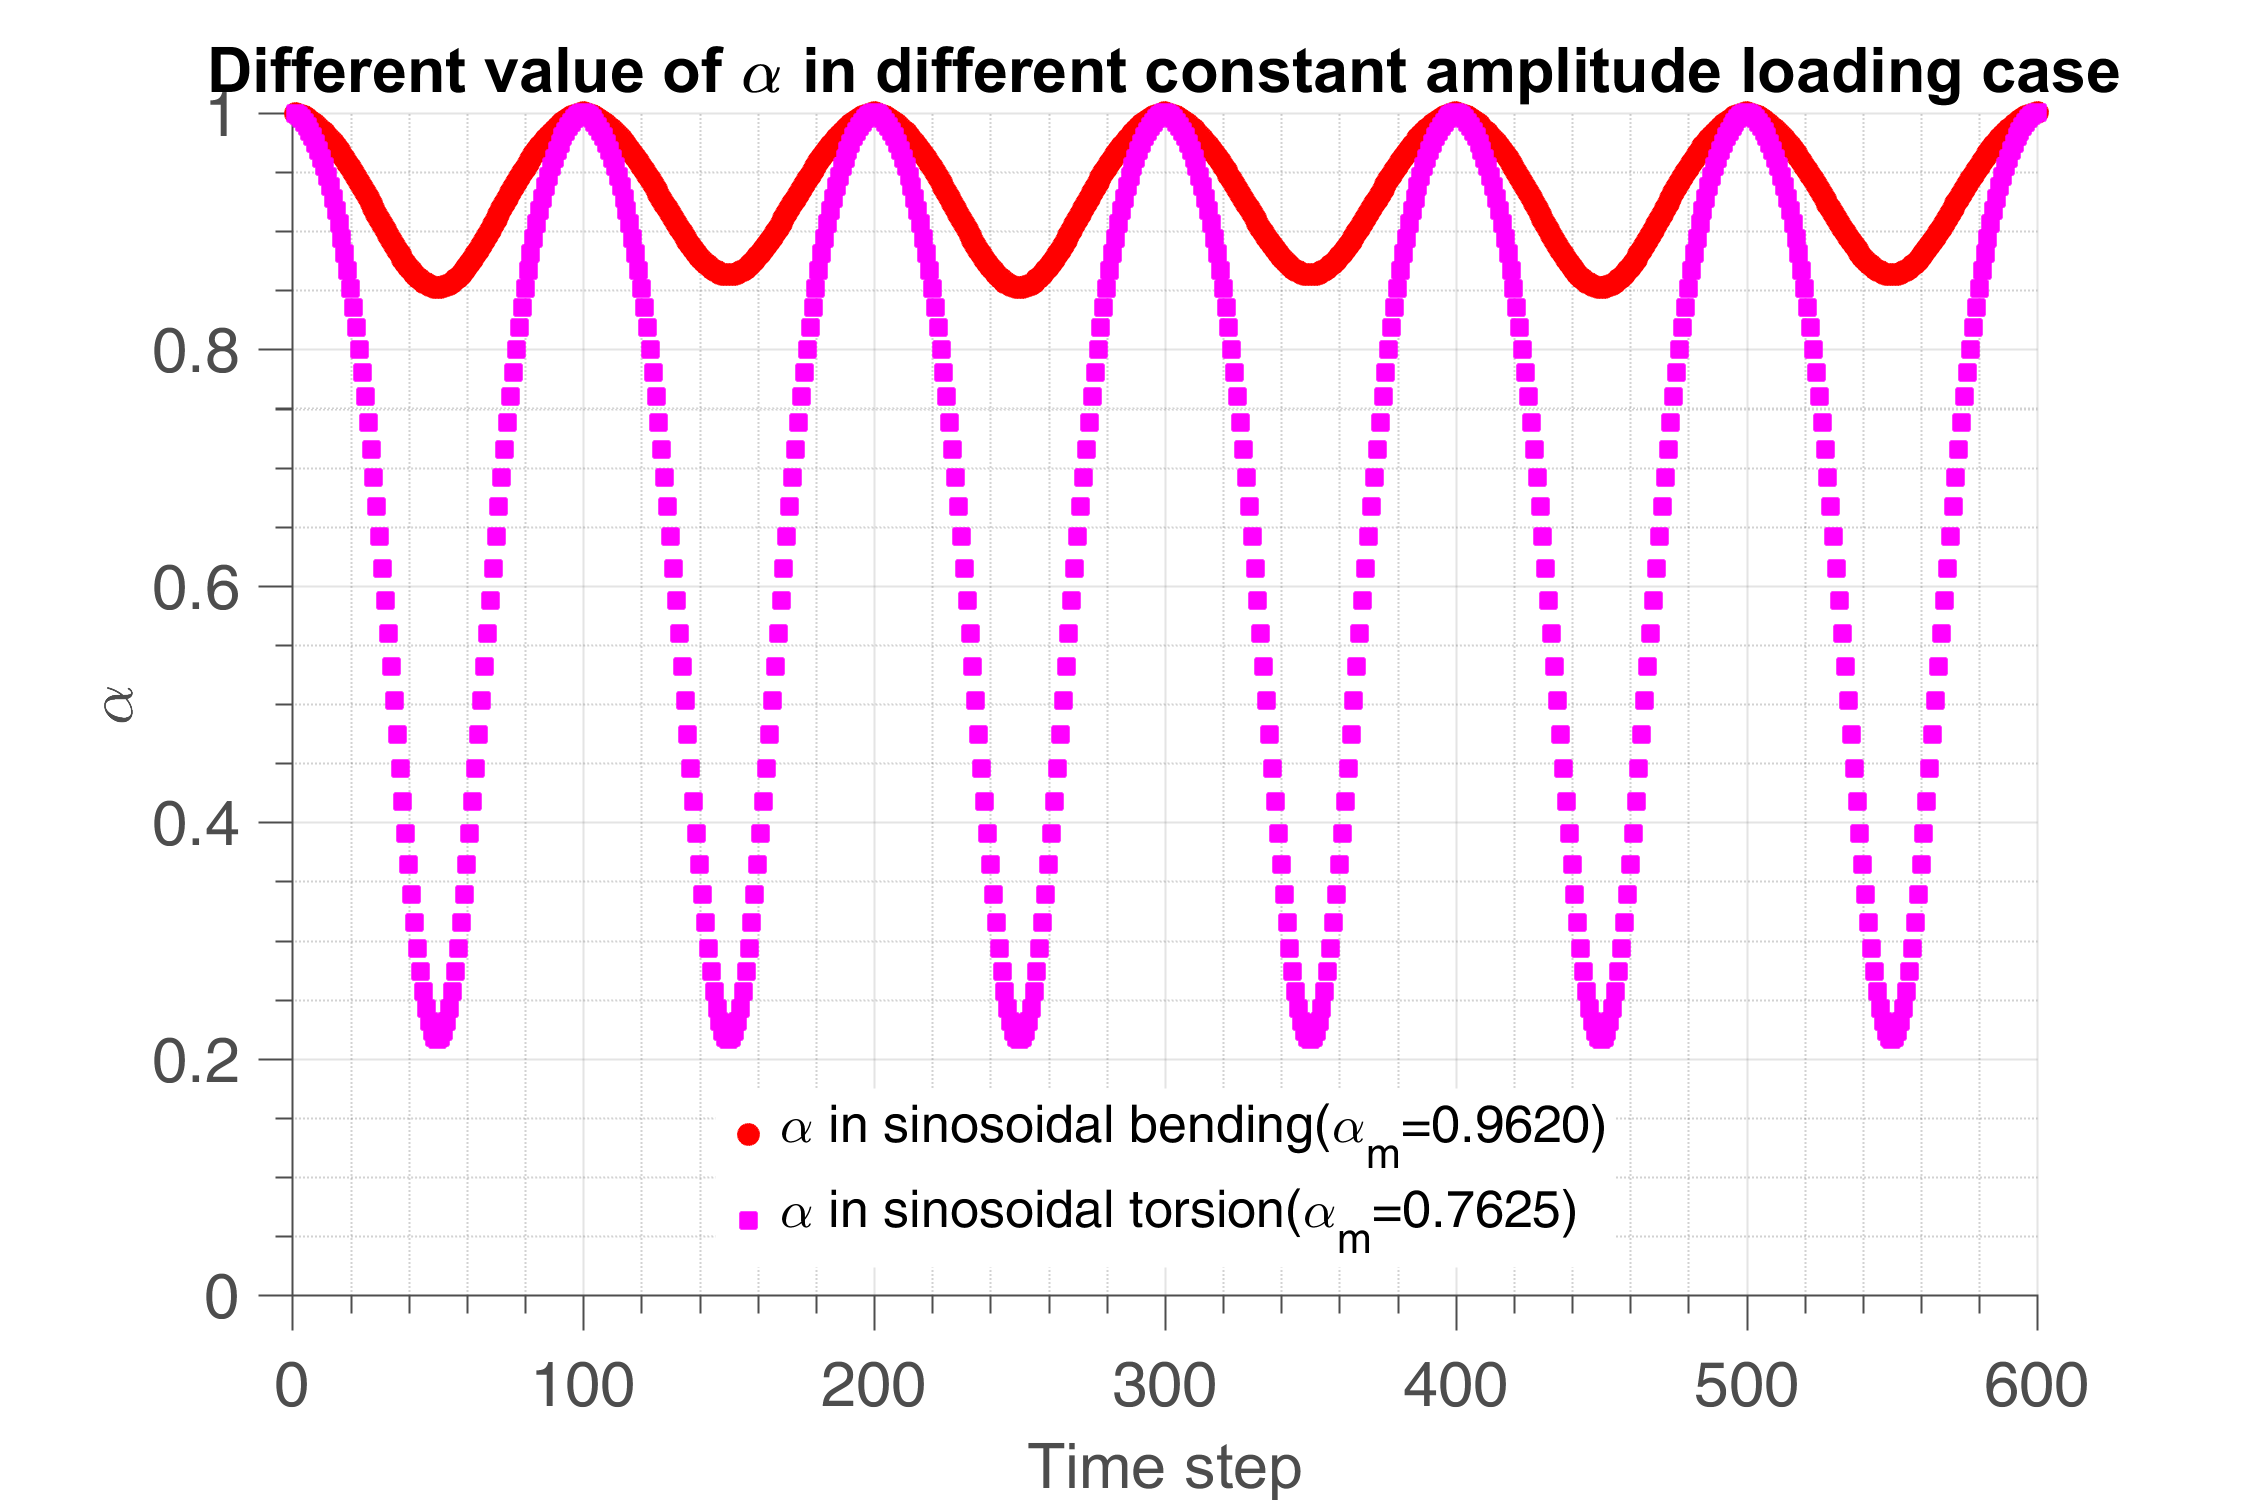
\includegraphics[width=0.8\textwidth]{figures//alp_mean_methods.png} 
	\caption{The evolution of $\alpha$ in bending and torsion with $\Sigma_y=1080 MPa$, $\Sigma_{bending}=\Sigma_{torsion}=500 MPa$, $a=0.3$ and $200$ time steps in one cycle}
	\label{fig.alpmean}
\end{figure}


Because of the possible large variations in time  of $\alpha$, the evolution problem in damage is very nonlinear and thus, one needs to develop and validate an improved numerical time integration strategy at least  for two specific cases: the constant amplitude case and the random load case.

We propose in constant amplitude load with very small evolution of damage per cycle to numerically calculate $W_{cyc}$ and the mean values of $\alpha$ through one cycle or several cycles(out-of-phase condition) and apply the result to life prediction by using  Eq.\eqref{eq.NFWcyc}:
\begin{equation}
N_F= \dfrac{W_0}{\left( 1-\alpha_m\right) W_{cyc}},
\label{eq.cycNF}
\end{equation}
which is obtained by direct integration of our damage law assuming time uniform dissipation in one cycle and frozen $\alpha$.
In this way the numerical cost is not as high as for the numerical implementation of all the loading points in random loading case. Because of the symmetrical shape of the evolution of $\alpha$, numerically the mean value of $\alpha$ does not strongly depend on the number of steps per cycle. In the verification process we have compared $100\sim1000$ time steps per cycle (\figref{fig.sn-num-ana}). 

For complex cyclic load cases, the idea is to accurately compute the history of plastic dissipation during one cycle (multiscale calculation with time refinement), and to use this precomputed result in the time integration of the scalar damage evolution law with a time stepping which is adapted to the time variation of $\alpha$. 

\begin{figure}[!h]
	\centering
	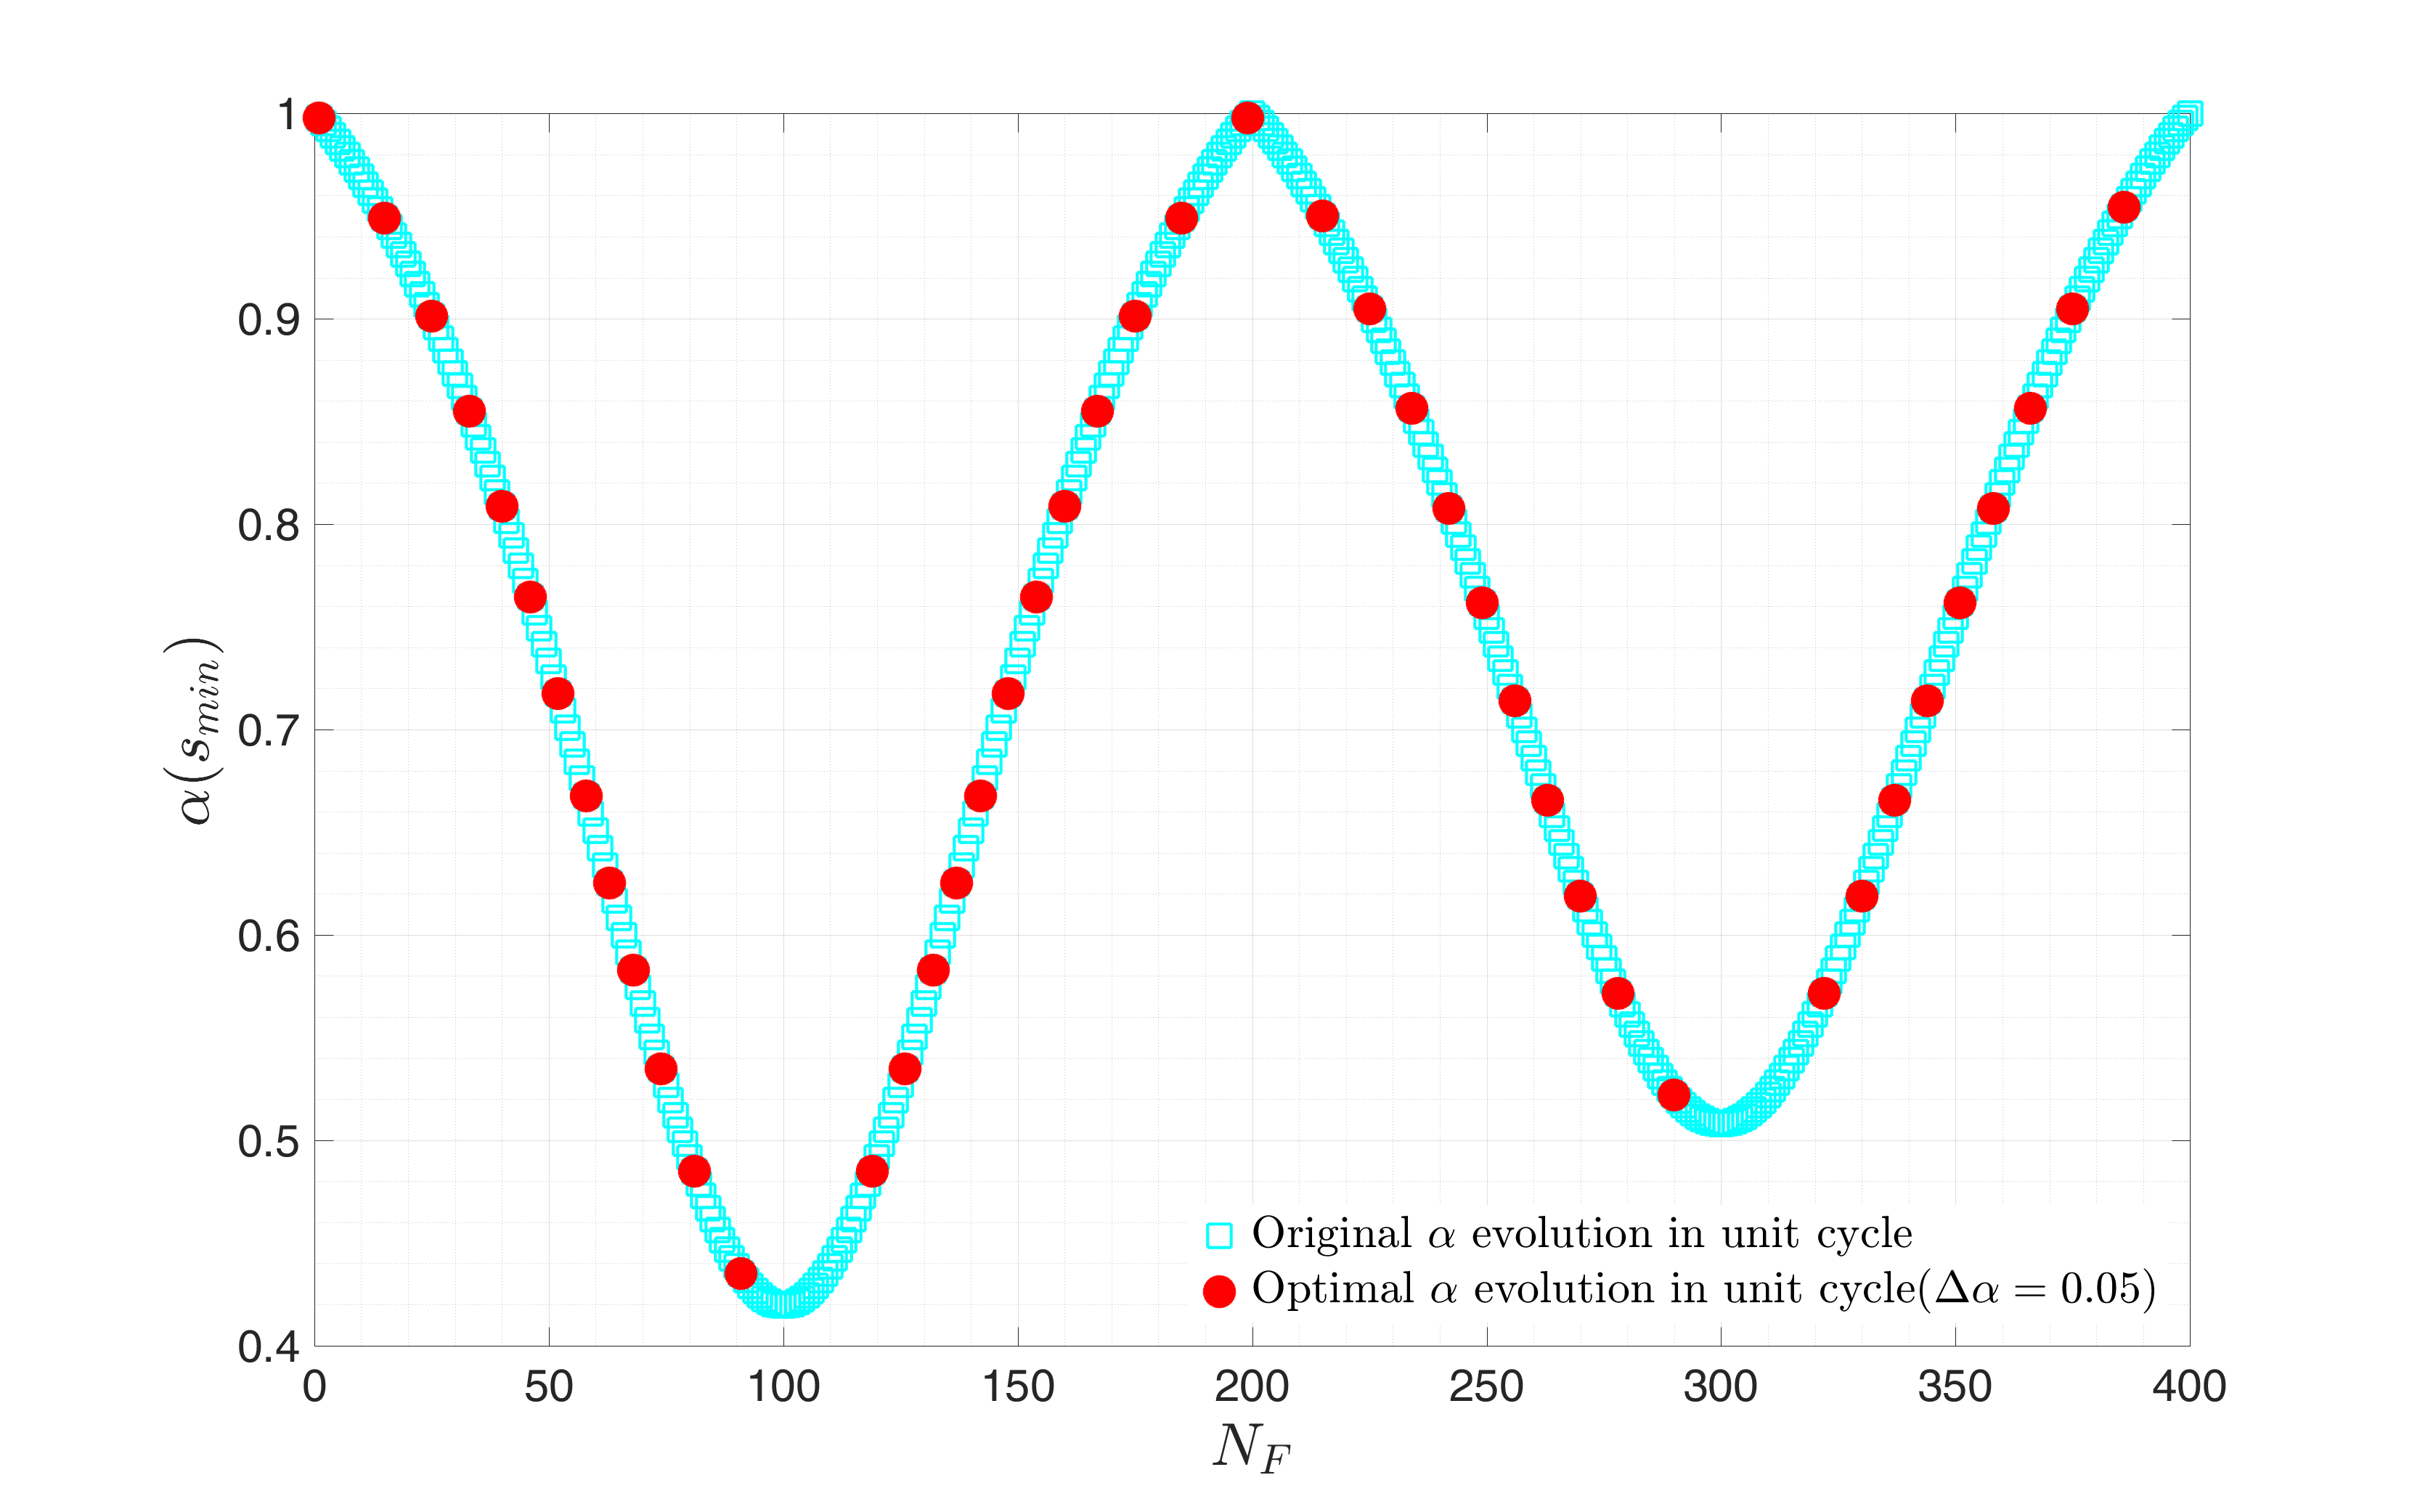
\includegraphics[width=0.8\textwidth]{figures//alpha_opt_vs_alpha_stepnumber.png} 
	\caption{Comparing numerical strategy with optimal time steps in one cycle with the old one, in this way the number of steps in unit cycle is reduced from 400 to 35, meaning a cost reduction factor of 0.0875 (with $\Delta\alpha=0.05$, $a=0.4$, $\lambda=0.1$, $\Sigma_y=230 MPa$, $\Sigma_{bending}=225 MPa$)}
	\label{fig.alpha_opt_vs_alpha_stepnumber}
\end{figure}

If $\alpha$ varies significantly, we use optimal time step numerical method to update $D$ during one time step. In more details, let us suppose that our first few cycles calculation with fine time steps $\Delta t$ has produced a sequence $\alpha(i)$ and $W_{cyc}(i)$ of exponent and dissipation at time $i\Delta t$. We then construct an adaptive time stepping strategy with variable time steps $\Delta t_{ref}(j)$, reference exponent $\alpha_{ref}(j)$ and dissipated energy $W_{ref}(j)$ by regrouping together adjacent time steps $\Delta t(i)$ with similar exponents $\alpha(i)$. This sequence is incremented as follows.


For $t_{ref}(j)$ and $\alpha_{ref}(j)=\alpha(t_{ref}(j))$ given, we set
$$\Delta t_{ref}(j)=\sum_{\substack{t(i)\geqslant t_{ref}(j)\\\left\| \alpha(i)-\alpha_{ref}(j)\right\|\leqslant \Delta\alpha }}\Delta t, \quad t_{ref}(j+1)=t_{ref}(j)+\Delta t_{ref}(j).$$
The same goes for the dissipated energy:
$$\Delta W_{ref}(j)=\sum_{\substack{t(i)\geqslant t_{ref}(j)\\\left\| \alpha(i)-\alpha_{ref}(j)\right\|\leqslant \Delta\alpha} }W_{cyc}(i) , \quad W_{ref}(j+1)=W_{ref}(j)+\Delta W_{ref}(j).$$

We finally use these new time steps with corresponding $\alpha_{ref}$ and $W_{ref}$ to update the damage by looping on all the following cycles with the new optimal time steps $j$ and cycles $N$, and updating damage in each cycle by:
\begin{equation}
D=D+D^{\alpha_{ref}(j)}\dfrac{\Delta W_{ref}(j)}{W_0},
\label{eq.optimal}
\end{equation}

with values $\alpha_{ref}(j)$ and $\Delta W_{ref}(j)$ precomputed in the first few cycles. This strategy is validated in \figref{fig.alpha_opt_vs_alpha_stepnumber}.

\vspace{6pt}
\textbf{Complexity analysis}
\vspace{6pt}

The optimal time step method clearly reduces the numerical cost. Typically, we assume the material has fatigue life of $1\times10^{6}$ cycles to failure and we implement $1000$ time steps in unit cycle. The reduction factor of points in unit cycle for example as in \figref{fig.alpha_opt_vs_alpha_stepnumber} equals $35/400=0.0875$. We can then compare the cost between full numerical strategy and the new one.

\begin{table}[!h]
\centering
\begin{tabular}{l|l}
\hline
Full numerical strategy: & $1000$ time steps $\times$ $64$ scales $\times$  $1\times10^{6}$ cycles       \\ \hline
Optimal cyclic strategy: & \begin{tabular}[l]{@{}l@{}} $1000$ time steps $\times$ $64$ scales $\times$  $5$ cycles until stabilization  \\$+$ $1\times10^{6}$ cycles $\times$ ($1000$ time steps $\times$ reduction factor)      \end{tabular}  \\ \hline
Ratio between optimal and full: & $\approx \dfrac{reduction \; factor}{64 \; scales}=\dfrac{1}{731}$       \\ \hline
\end{tabular}
\end{table}

The same strategy is applied to random loading situations which are made of repeated sequence of random loads:

\begin{itemize}
	\item calculation of dissipated energy and exponent on one sequence;
	
	\vspace{6pt}	
	
	\item time coarsening;
	
	\vspace{6pt}	
	
	\item repeated integration of damage through the different sequences using Eq.\ref{eq.optimal}.
		
	\vspace{6pt}
\end{itemize}
                          
In such a strategy, the extra cost of introducing multiple scales in the calculation becomes negligible as compared to the time integration of damage in the evolution process.

\begin{Figure}[]{S-N curve of bending test on 30NCD16 steel using numerical and analytical method (Eq.\eqref{eq.cycNF}) with different time steps. Data are those of table.\ref{tab:Sin}}[fig.sn-num-ana]
	\centerline{
		\graphfile*[38]{figures//SN_num_ana_stepnumber=30.png}[30 time steps in unit cycle($\beta=1.1$, $a=0.001$).]
		\graphfile*[38]{figures//SN_num_ana_stepnumber=100.png}[100 time steps in unit cycle($\beta=1.1$, $a=0.001$).]}
	\\
	\centerline{
		\graphfile*[38]{figures//SN_num_ana_stepnumber=30_err.png}[Relative error$\left( \dfrac{NF_{num}-NF_{analytical}}{NF_{analytical}}\right)$  with 30 time \protect \\ steps in unit cycle  ($\beta=1.1$, $a=0.001$)]
		\graphfile*[38]{figures//SN_num_ana_stepnumber=100_err.png}[Relative error$\left( \dfrac{NF_{num}-NF_{analytical}}{NF_{analytical}}\right)$   with 100 time \protect \\ steps in unit cycle  ($\beta=1.1$, $a=0.001$)]}
	\label{fig.sn-num-ana}
\end{Figure}

\newpage

Altogether, we have three numerical approaches for integrating damage.

\begin{enumerate}
	\item  Numerical results with varying $\alpha$(equally divide time in unit cycle), and do the scale integration all along the fatigue life time, which can be of high numerical cost$$\delta D=D^\alpha\frac{\dot{W}}{W_0}\delta t.$$
	This method only serves for qualification purposes.
	\vspace{6pt}
	
	\item  Numerical results with optimal time steps(equally divide $\alpha$in unit cycle), here we have $\Delta\alpha=0.01$, to reduce time steps needed, after several cycles adaptation we iterate using the recorded scalar values of $\alpha_{ref}$, $W_{ref}$ and $t_{ref}$ to decide fatigue life time.
	$$\delta D=D^{\alpha_{ref}}\frac{W_{ref}}{W_0}\delta t_{ref}.$$
	\vspace{6pt}
	
	\item  Analytical results after integration of D (with mean alpha from numerical strategy)$$N_F=\frac{W_0}{( 1-\alpha_m)W_{cyc}},$$ 
	which is derived from the differential equation
	$$\delta D=D^{\alpha_m}\frac{W_{cyc}}{W_0}\delta N.$$
\end{enumerate}	

Although method 2 is much more numerically efficient than the original numerical method 1, it is still not cheap in the experimental fitting process. We need the analytical formula method 3 to do the fitting process. To validate the feasibility, we now compare only the analytical(method 3) one and optimal time steps(method 2) one. The results are shown in \figref{fig.SNnumerical2methods} and \figref{fig.SNnumerical2methods2}, the relation ship between relative error and $\Delta \alpha$ with 2000 time steps in unit cycle is shown in  \figref{fig.errorNumAna0.02} and \figref{fig.errorNumAna0.01}.
\begin{figure}[!h]
	\centering
	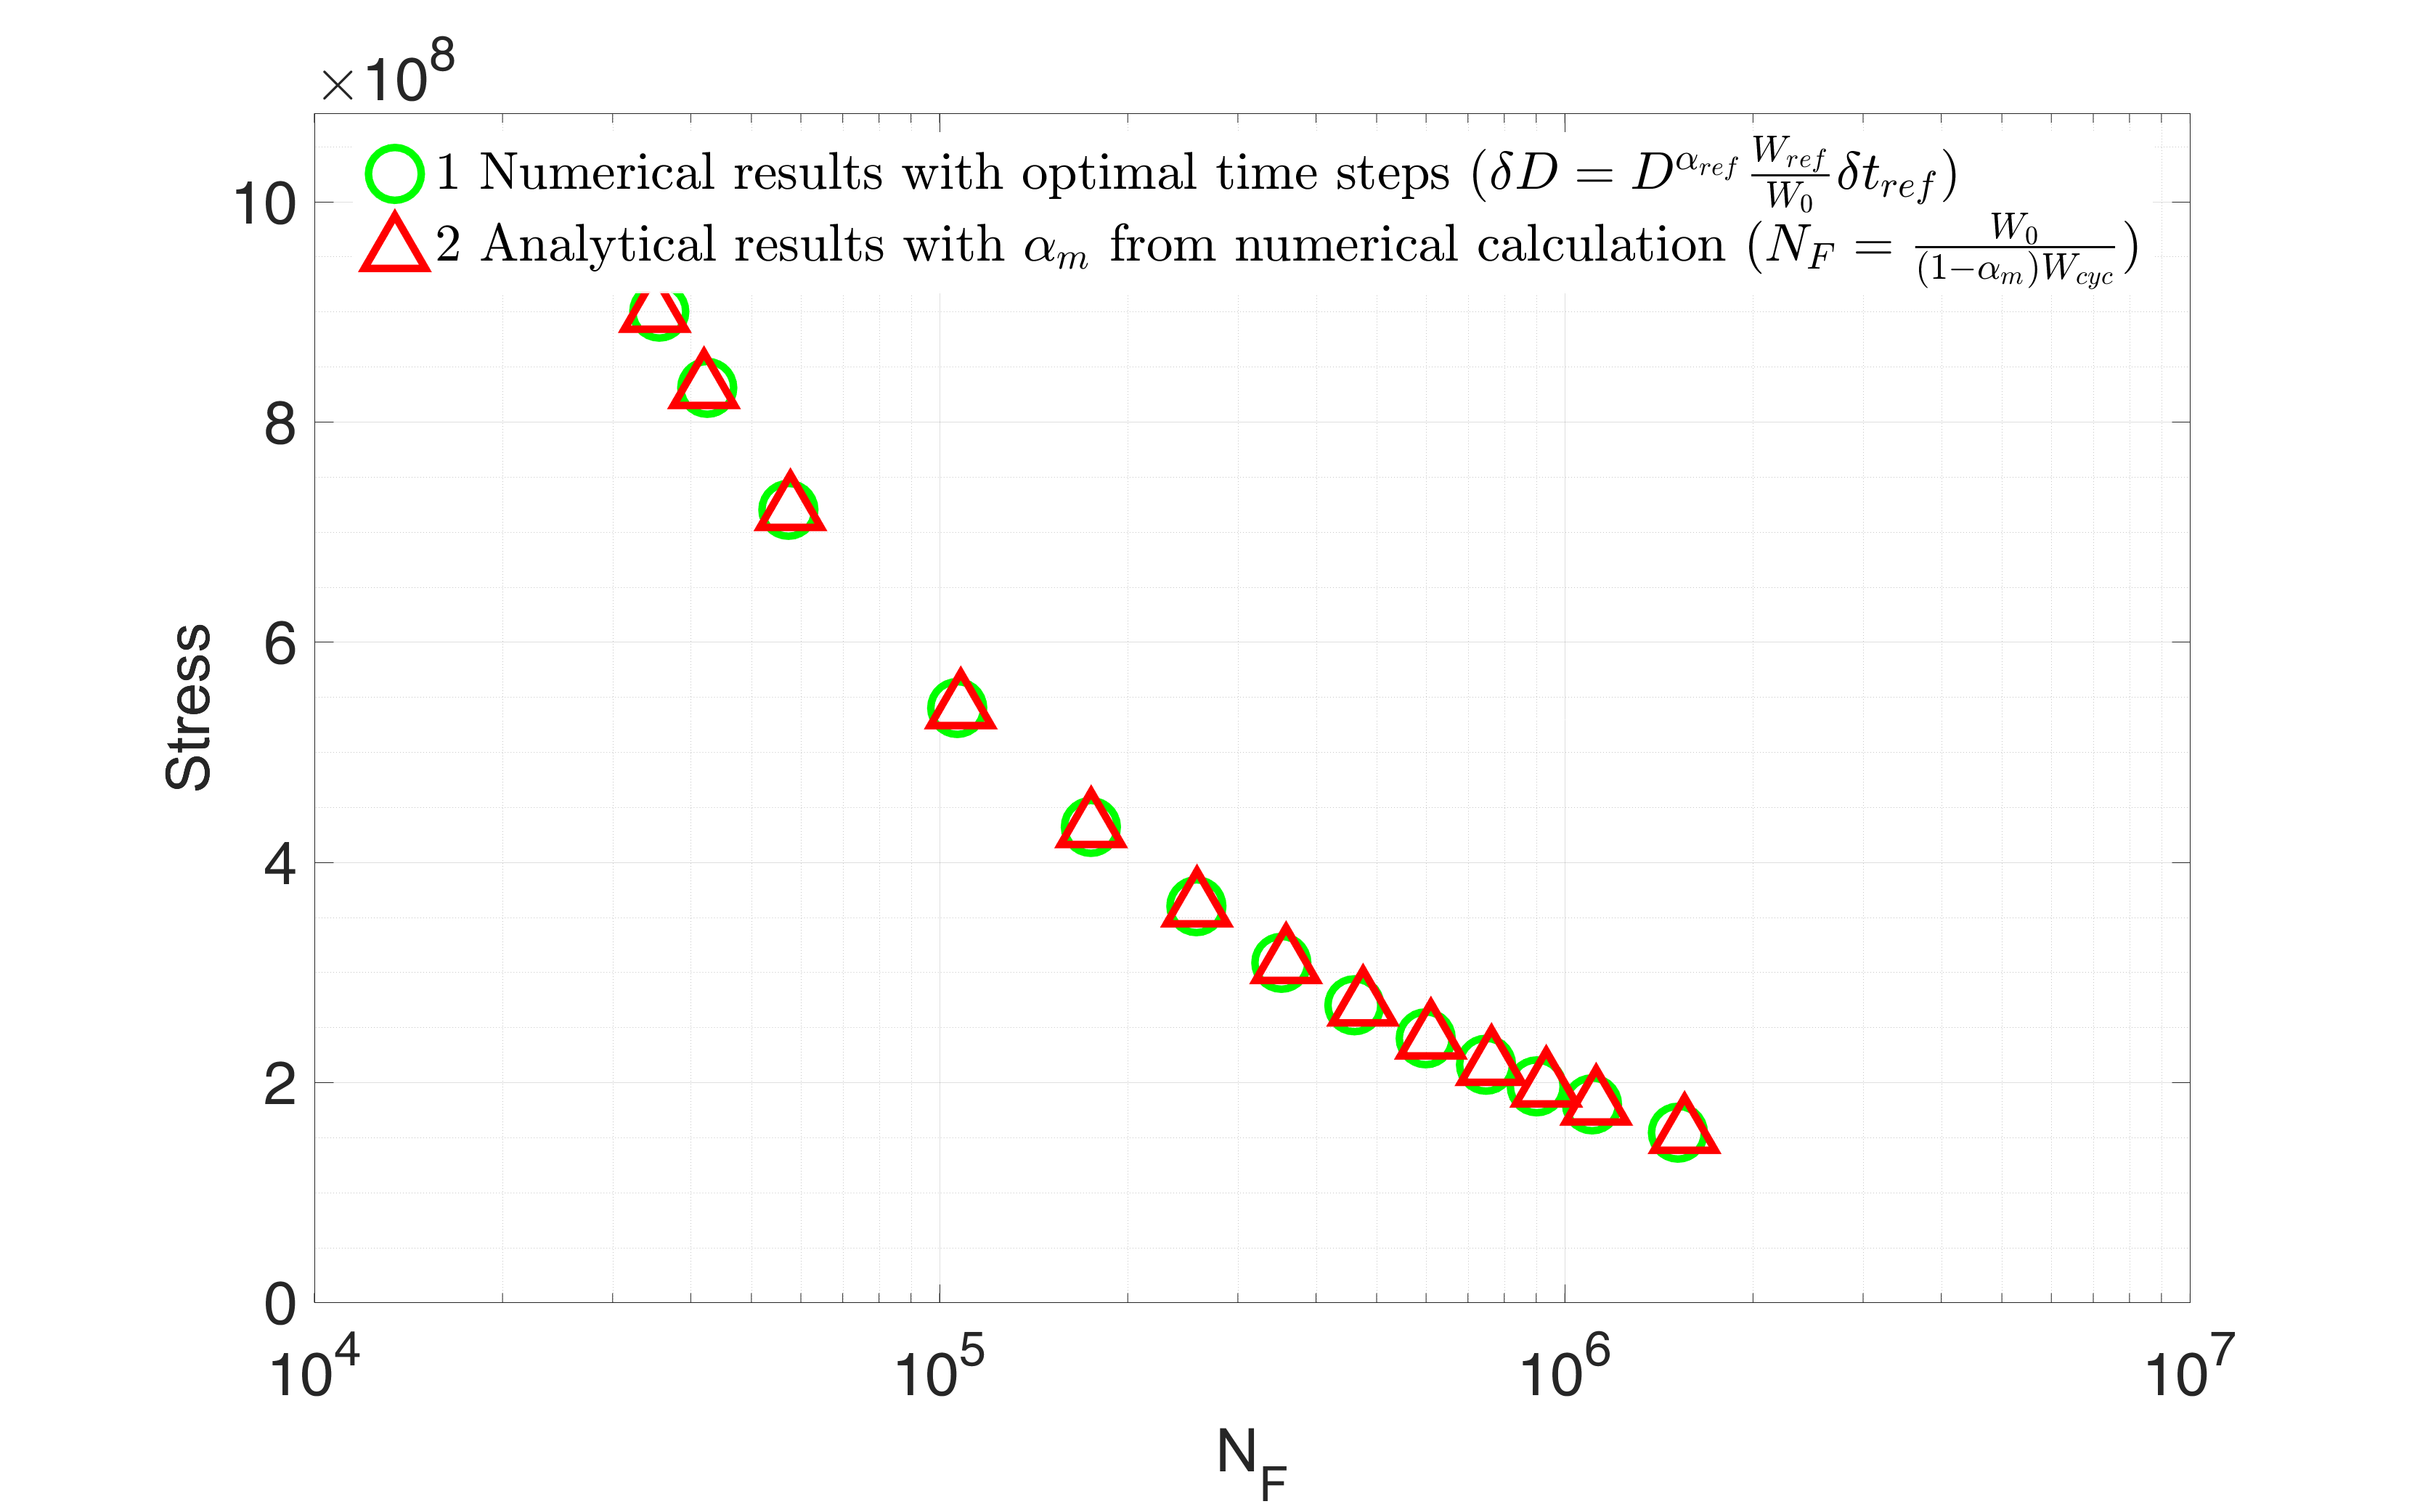
\includegraphics[width=\textwidth]{figures//SN_opt_ana_200_delta_alp=0.00002.png} 
	\caption{S-N curve using analytical and numerical results with optimal time steps methods ($\beta=1.1$, $a=0.01$, $\Delta \alpha=2E-5$ in unit cycle), yielding 200 full time steps reduced to 197 optimal time steps}
	\label{fig.SNnumerical2methods}
\end{figure}
\begin{figure}[!h]
	\centering
	\includegraphics[width=\textwidth]{figures//SN_opt_ana_200_delta_alp=0.00001.png} 
	\caption{S-N curve using analytical and numerical results with optimal time steps methods ($\beta=1.1$, $a=0.01$, $\Delta \alpha=1E-5$ in unit cycle), yielding 200 full time steps reduced to 199 optimal time steps}
	\label{fig.SNnumerical2methods2}
\end{figure}
\begin{figure}[!h]
	\centering
	\includegraphics[width=\textwidth]{figures//SN_opt_ana_200_delta_alp=0.00002_err.png} 
	\caption{Relative error $\left( \dfrac{NF_{opt}-NF_{analytical}}{NF_{analytical}}\right)$  between analytical and numerical results with optimal time steps methods ($\beta=1.1$, $a=0.01$, $\Delta \alpha=2\times10^{-5}$ in unit cycle)}	
	\label{fig.errorNumAna0.02}
\end{figure}
\begin{figure}[!h]
	\centering
	\includegraphics[width=\textwidth]{figures//SN_opt_ana_200_delta_alp=0.00001_err.png} 
	\caption{Relative error $\left(\dfrac{NF_{opt}-NF_{analytical}}{NF_{analytical}}\right)$  between analytical and numerical results with optimal time steps methods ($\beta=1.1$, $a=0.01$, $\Delta \alpha=1\times10^{-5}$ in unit cycle)}
	\label{fig.errorNumAna0.01}
\end{figure}

Now we can conclude that with more time steps in unit cycle, we get closer results with the original numerical method(method 2) in HCF regime. With smaller $\Delta \alpha$ value, we get less relative error between numerical(method 3) and analytical(method 1) results. This indicates that in constant amplitude cyclic loading, with moderate values of $\beta$ it is feasible to use the analytical formula, given $\alpha_m$ is calculated using sufficient large time steps and small $\Delta \alpha$ in the first several cycles.

\clearpage
\section{Validation on recovery tests}
\label{sec:5.8}
\subsection{Recovery of Chaboche law on cyclic loading}
The test is first performed on a sinusoidal uniaxial load $\Sigma_{11}(t)=Asin(t)$, giving a deviatoric amplitude$S_{a}(t)=\sqrt{J_{2,a}(dev\uuline{\Sigma(t)})}$  so that $S_{a}(t)=\left\| \sqrt{\dfrac{1}{3}}\Sigma_{11}(t)\right\| $. We use parameters in Table.\ref{tab:Sin} to recover the classic Chaboche law in cyclic loading.
\begin{table}[!h]
\centering
\begin{tabular}{ll}
\hline
\textbf{Parameters}                                         & \textbf{Value}                    \\ \hline
Young's modulus                                             & $E=191$ GPa                       \\
Hardening parameter                                         &  $k=1$ GPa \\
Weakening scales distribution exponent                      & $\beta=1.5$                             \\
Hydrostatic pressure sensitivity                            & $\lambda_{+-}=0.6$                     \\
Macroscopic yield stress                                    & $\sigma_y=1080$ MPa              \\
Sequencing effect sensitivity                               & $a=0.1$                        \\
Dissipated energy to failure per unit volume                & $W_0=5$ MJ(MPa)                       \\ \hline
\end{tabular}
\caption{Material parameters in a simple cyclic load }
\label{tab:Sin}
\end{table}

We use matlab to numerically realize our method. The plot of $\left\|  \uline{\uline{S}}-\uline{\uline{b}}\right\|_{trial}$ and $\left\|  \uline{\uline{S}}-\uline{\uline{b}}\right\|$ during the first cycles at two different scales($s_{3}=1.21$ and $s_{10}=1.13$) are shown in \figref{fig.trialsin0} and \figref{fig.trialsinm}. We use here a fixed value of $\lambda$($\lambda_+=\lambda_-$), thus the local yield limit is reduced in traction and increased
in compression.

\begin{figure}[!h]
\centering
\includegraphics[width=\textwidth]{figures//trialsin_0.png} 
\caption{Microscopic $\left(  \uline{\uline{S}}-\uline{\uline{b}}\right)_{trial}$ and $\left( \uline{\uline{S}}-\uline{\uline{b}}\right)$ evolution with time under different weakening scales($s_{3}=1.21$ and $s_{10}=1.13$) in sinusoidal load with zero mean stress}
\label{fig.trialsin0}
\end{figure}
\begin{figure}[!h]
\centering
\includegraphics[width=\textwidth]{figures//trialsin_m.png} 
\caption{Microscopic $\left(  \uline{\uline{S}}-\uline{\uline{b}}\right)_{trial}$ and $\left( \uline{\uline{S}}-\uline{\uline{b}}\right)$ evolution with time under different weakening scales($s_{3}=1.21$ and $s_{10}=1.13$) in sinusoidal load with mean stress=300 MPa}
\label{fig.trialsinm}
\end{figure}

The time history of dissipated energy is depicted in \figref{fig.W3methods}. We scale $S_{a}$ in the plot to see more clearly the relation between energy dissipation and stress intensity. The choice of $\alpha$ does not affect $W$; it only concerns damage accumulation rate. Smaller $\alpha$ causes faster accumulation.

The ``jump'' in energy evolution is due to activation of new scales while in-between two scales the dissipated energy follows the stress increment at each time step. In other words, because in our method the dissipated energy $W$(\figref{fig.W3methods}), sums energy dissipation at all scales, any additional violation of $\left\|S-b \right\|_{trial}$ at local yield limit(\figref{fig.trialsin0}) introduces an additional dissipation. 

\begin{figure}[!h]
\centering
\includegraphics[width=0.95\textwidth]{figures//W_3methods.png} 
\caption{Validation of dissipated energy in all scales with analytical(method 3) and numerical method(method 1) with $\beta=1.1$,$\Sigma=0.85\sigma_y$. The time evolution of $\alpha$ does not play a role in the dissipation calculation which is normal since $\alpha$ does not enter in the dissipation calculation }
\label{fig.W3methods}
\end{figure}
\begin{figure}[!h]
	\centering
	\includegraphics[width=0.95\textwidth]{figures//W_3methods_enlarge.png} 
	\caption{Validation of dissipated energy in all scales with analytical and numerical method(enlargement of \figref{fig.W3methods})}
	\label{fig.W3methodsenlarge}
\end{figure}
\begin{figure}[!h]
\centering
\includegraphics[width=0.95\textwidth]{figures//W_3methods2_100steps.png} 
\caption{Dissipated energy accumulation through time with different methods, there are 100 time steps in unit cycle}
\label{fig.W3methods100}
\end{figure}
\begin{figure}[!h]
\centering
\includegraphics[width=0.95\textwidth]{figures//W_3methods_100steps_enlarge.png} 
\caption{Dissipated energy accumulation through time with of 3 methods(enlargement of \figref{fig.W3methods100})}
\label{fig.W3methods2enlarge}
\end{figure}
\begin{figure}[!h]
\centering
\includegraphics[width=0.95\textwidth]{figures//W_3methods_diff_100steps.png} 
\caption{Relative difference $\dfrac{W_{analytical}-W_{numerical}}{W_{analytical}}$ between analytical energy loss and numerical one with $\alpha$ varying with time of \figref{fig.W3methods100}}
\label{fig.W3methodsdiff}
\end{figure}
\begin{figure}[!h]
\centering
\includegraphics[width=\textwidth]{figures//D_3methods2_100steps.png} 
\caption{Damage evolution with time under sinusoidal load with different methods, there are 100 time steps in unit cycle($\beta=1.1$,$\Sigma=0.85\sigma_y$)}
\label{fig.damsin100}
\end{figure}

\begin{figure}[!h]
\centering
\includegraphics[width=\textwidth]{figures//D_3methods_100steps_enlarge.png} 
\caption{Damage evolution with time under sinusoidal load with two different methods(enlargement of \figref{fig.damsin100})}
\label{damsinenglarge}
\end{figure}

\begin{figure}[!h]
\centering
\includegraphics[width=\textwidth]{figures//D_3methods_diff_100steps.png} 
\caption{Relative difference $\dfrac{D_{analytical}-D_{numerical}}{D_{analytical}}$ evolution with time of \figref{fig.damsin100}}
\label{Damagediff}
\end{figure}
We take the mean value of $\alpha$ during all the iteration process of numerical method as $\alpha_{m}$. The energy and damage accumulation is shown in \figref{fig.W3methods100} and \figref{fig.damsin100}. Here we give 100 time steps in one cycle to see the relative difference between changing $\alpha$ and $\alpha_{m}$, also $\dot{W}$ and $W_{cyc}/stepnumber$  method. The more time steps we give, the more precision we get. The relative difference between analytical energy loss and numerical one is shown in \figref{fig.W3methodsdiff} from which we conclude that the three methods converge in terms of elastic energy dissipation, but due to nonlinear effects the damage evolution does not have the same history per cycle. The frozen $\alpha$ delays damage, the varying $\alpha$ increases damage during the phase of strong loading. The difference has a significant impact if damage occurs with very few cycles. It will not when computing on a large number of cycles.

The cyclic load calculation is only valid for very simple such as proportional loading in fatigue. However, the convergence of the two methods is based on the small value of $\beta$(close to 1), in case of large values of $\beta$(typically around 5), the numerical strategy gives shorter life than the analytical one due to extreme non-linearity in the energy dissipation history per cycle. The relative error is around 20\% as shown in \figref{fig.W3methods_bigbeta_04y} and \figref{fig.W3methods_bigbeta_08y}. Nevertheless the analytical formula can still be used as a comparison group to verify the numerical results. And in the identification process we need the analytical form to fit the $S-N$ curve of a certain material. The outcome is satisfactory. Hence, to be more general for any loading history, we adopt the numerical method after identification of $\beta$. 

\begin{figure}[!h]
	\centering
	\includegraphics[width=0.95\textwidth]{figures//W3methods_bigbeta_04y.png} 
	\caption{Validation of dissipated energy in all scales with analytical and numerical method with $\beta=5$, $\Sigma=0.4\sigma_y$ }
	\label{fig.W3methods_bigbeta_04y}
\end{figure}
\begin{figure}[!h]
	\centering
	\includegraphics[width=0.95\textwidth]{figures//W3methods_bigbeta_08y.png} 
	\caption{Validation of dissipated energy in all scales with analytical and numerical method with $\beta=5$, $\Sigma=0.8\sigma_y$ }
	\label{fig.W3methods_bigbeta_08y}
\end{figure}
\begin{figure}[!h]
	\centering
	\includegraphics[width=\textwidth]{figures//damsin_bigbeta_04y.png} 
	\caption{Damage evolution with time under sinusoidal load with $\beta=5$, $\Sigma=0.4\sigma_y$. In such a severe loading and with extreme non-linearity, the simple Chaboche like formula with frozen $\alpha$ departs from the outcome of the full numerical model}
	\label{fig.damsin_bigbeta_04y}
\end{figure}
\begin{figure}[!h]
	\centering
	\includegraphics[width=\textwidth]{figures//damsin_bigbeta_08y.png} 
	\caption{Damage evolution with time under sinusoidal load with $\beta=5$, $\Sigma=0.8\sigma_y$}
	\label{fig.damsin_bigbeta_08y}
\end{figure}

\clearpage
\subsection{Numerical recovery of sequence effect}
We adopt the parameter $\alpha$ to take into account the sequence effect. The high-low loading sequence clearly reduces the fatigue life, as depicted in \figref{fig.sequencesigalpd}. In order to cover this phenomenon, we let $\alpha$ change with time($\alpha=1-a\left( s_{min}(t)-1\right)^{-f}$). Here $a$ is the sequence effect sensitivity. According to Eq.\eqref{eq.smin}, we have:
$$
s_{min}(t)=\dfrac{\Sigma_y-\lambda \Sigma_H(t)}{S_{a}(t)},
$$
which is the minimum weakening scale that activates energy loss.  We use a general law for $\alpha$ of the type $\alpha = \alpha (s_{min})$ with the idea that for us $s_{min}$ is a measure of present intensity of macroscopic stress. It is therefore a mechanical based stress norm. The impact of this construction of $\alpha$ can be seen on \figref{fig.randomdispersion}, on a test case specifically built to illustrate such a sequence effect.

\begin{Figure}[]{Two level sequence effect. By comparing the vertical figures we can see high stress gives high $(1-\alpha)$ value which causes fast damage accumulation speed. The evolution of $(1-\alpha)$ is highly nonlinear and follows the value of stress at each time step.}[fig.sequencesigalpd]
\centerline{
\graphfile*[40]{figures//high-low-Smax.png}[]
\graphfile*[40]{figures//low-high-Smax.png}[]}
\\
\centerline{
\graphfile*[40]{figures//high-low-alp.png}[]
\graphfile*[40]{figures//low-high-alp.png}[]}
\\
\centerline{
\graphfile*[40]{figures//high-low-D.png}[]
\graphfile*[40]{figures//low-high-D.png}[]}
\label{fig.sequencesigalpd}
\end{Figure}


\clearpage
\subsubsection{Major damage effect}

To see the influence of sequence effect factor of $\alpha$, we first fix $\alpha$ for all tests to see the results. When $\alpha$ is fixed, it becomes denominator in the final expression of $N_F$ (Eq.\eqref{eq.NFWcyc}) and has the same impact as $W_0$. We find  that the fatigue life of random loading is widely dispersed (\figref{fig.randomdispersion}). In this case we need to use $\alpha=f(s_{min})$ which evolves with time to make large stress intensity bring more damage.

\begin{figure}[!h]
	\centering
	\includegraphics[width=\textwidth]{figures//randomdispersion.png} 
	\caption{Fatigue life of random loading dispersion}
	\label{fig.randomdispersion}
\end{figure}

After comparison with the experimental data we find out that large stresses cause much more damage than the smaller ones. It is necessary to include this major stress induced damage to our stress intensity parameter $\alpha$. With the new $\alpha$ used in Eq.\eqref{eq.final3} compared to Eq.\eqref{eq.alpha} we are able to calibrate our model better with the experimental results by using 
\begin{equation}
\alpha=1-a\left(  \dfrac{\frac{1}{s_{min}}}{1-\frac{1}{s_{min}}} \right) ^{f}.
\label{eq.majoralp}
\end{equation}


With $f=1.1$, we use the power to magnify large stress impact and minify lower stress damage.  The demonstration of major damage effect using magnification power is depicted in \figref{fig.sequenceours}. With larger value of power, the sequence effect is more significant(bigger dispersion between high-low and low-high sequence).

\begin{figure}[!h]
\centering
\includegraphics[width=\textwidth]{figures//sequence_ours.png} 
\caption{Major damage effect using different magnification power of Eq.\eqref{eq.majoralp} on sequence effect. Here high stress is 1MPa and low stress is 0.8MPa. We see that using a large power $f$ in Eq.\eqref{eq.majoralp} induces a stronger sequence effect.}
\label{fig.sequenceours}
\end{figure}

The larger value of $S_{a}$ causes more damage in the presence of the power $\beta$, leading to faster increase of 
$$(1-\alpha)=a\left(  \dfrac{\frac{1}{s_{min}}}{1-\frac{1}{s_{min}}} \right) ^{f}=a(s_{min}-1)^{-f}.$$ 
which causes faster damage accumulation. We can also see this effect in \figref{fig.SmaxSequence}. 

To assess large stress correctly we define the larger stress intensity as the value of stress which makes expression in the bracket in the second term of $\alpha$ greater than 1($ \dfrac{1}{ s_{min}(t)-1 }>1$), then we use power $\beta$ to magnify this term. In this way the damage is accelerated for large stresses. The deviatoric stress $S_{a}$, above which the damage is magnified,  is determined from: 
$$\alpha(t)=1-a\left( \dfrac{1}{ s_{min}(t)-1 } \right)^{1.1},$$
$$s_{min}(t)=\dfrac{\Sigma_y-\lambda \Sigma_H(t)}{S_{a}(t)}<2,$$
$$S_{large}(t)>\dfrac{\Sigma_y-\lambda \Sigma_H(t)}{2}.$$ 

The major damage effect can be seen in \figref{fig.SmaxSequence}, which occurs when $S$ is more than half the macroscopic yield stress of the material.

\begin{figure}[!h]
\centering
\includegraphics[width=\textwidth]{figures//alp_Smax_fb.png} 
\caption{(1-$\alpha$) term which stands for the load intensity evolution, both with and without the magnification power $f$}
\label{fig.SmaxSequence}
\end{figure}

\clearpage
\section{Identification strategy}
\label{sec:5.9}
In our tests we keep $f=1.1$(justified in Chapter \ref{chp:6} by \figref{fig.Cetimerralpfix} and \figref{fig.Cetimerr}). The positive hydrostatic stress and negative one have different effect on the yield limit. It is necessary to adopt 2 parameters to describe this behavior. So we divide the hydrostatic sensitivity $\lambda$ into 2 parts. $\lambda_+$ and $\lambda_-$. In the analytical formula, the amplitude of the stress intensity is adopted and the average value of tension hydrostatic stress(+) and compressive hydrostatic stress(-) is introduced.

For a good lifetime prediction, it is necessary to first identify the appropriate parameters of the model. For this purpose, we use the analytical formula Eq.\eqref{eq.cycNF} obtained in uniaxial cyclic loading case. With distinction of the hydrostatic stress in the presence of non-zero mean stress and since in fully reversed uniaxial loading we spend an equal time in compression and in traction, Eq.\eqref{eq:w} now writes:

\begin{equation}
W_{cyc}=\dfrac{2(E-k)(1+\nu)\left( \beta-1\right) }{ E(E+k\nu)\beta\left( \beta+1\right) }\left[ \dfrac{S_{a}^{\beta+1}}{ \left(\sigma_y-\lambda_+ \overline{\Sigma}_{H+}(t)\right)^{\beta-1}}+\dfrac{S_{a}^{\beta+1}}{ \left(\sigma_y-\lambda_- \overline{\Sigma}_{H-}(t)\right)^{\beta-1}}\right] .
\label{eq:wcycnew}
\end{equation}

\begin{equation}N_{Fnum}=\dfrac{W_0}{\left( 1-\alpha\right) }\dfrac{E(E+k\nu)\beta\left( \beta+1\right) }{ 2(E-k)(1+\nu)\left( \beta-1\right) }\dfrac{1}{\dfrac{S_{a}^{\beta+1}}{\left(\sigma_y-\lambda_+\overline{\Sigma}_{H+}(t)\right)^{\beta-1}}+\dfrac{S_{a}^{\beta+1}}{\left(\sigma_y-\lambda_-\overline{\Sigma}_{H-}(t)\right)^{\beta-1}}}.\label{eq:NFnew}
\end{equation}


To use our analytical model Eq.\eqref{eq:NFnew} to fit the experiments, we employ matlab Least-Squares (model fitting) algorithm. 

The best fitted parameters in uniaxial cyclic loading case are deduced from the minimization of the sum of square of difference between uniaxial numerical and experimental results:
\begin{equation}
\min_{\beta,\lambda,W_0}\left\lbrace \sum_{i}\left(N_{Fnum}-N_{Fexp} \right)^2\right\rbrace 
\label{eq.leastsquares}
\end{equation}

Assume there are $i$ sets of experimental data. To clarify the identification process, let us separate the parameters into:
\begin{itemize}
	\item Experimental data: $S_{a(i)}$, $\Sigma_{H(i)}$, $N_{Fexp(i)}$, $\sigma_y$, $E$, $k$, $\nu$.
	\item Material constants: $\beta$, $\lambda_{+-}$, $W_0$ (to be fitted)
	\item Input data from experimental data: $S_{max(i)}$, $\Sigma_{H(i)}$
	\item Input data from experimental data and parameter constants: $\alpha_{(i)}$
	\item Output data: $N_{Fnum(i)}$
\end{itemize}

In this process, $\sigma_y$, $E$, $k$ and $\nu$ are given elastoplastic material constants. For each test (i), the load parameters are maximum amplitude $S_{a(i)}$, mean hydrostatic stress $\overline{\Sigma}_{H(i)}$, and the experimental number of cycles to failure is given by $N_{Fexp(i)}$.

The exponent $\alpha_{(i)}$ is cycle average obtained by
\begin{equation}
\alpha_{(i)}=mean\left[1-a\left( \dfrac{1}{\dfrac{\Sigma_y-\lambda_{+-} \Sigma_{H}(t)}{S_{a}(t)}-1 } \right)^{1.1}\right] (i).
\label{eq.meanalp}
\end{equation}

The parameters to be calibrated are $W_0$, $\beta$ and $\lambda$. Since the exponent $\alpha_{(i)}$ depends on $\beta$ and $\lambda$, we proceed iteratively by:

\begin{enumerate}
	\item We first identify the S-N curve slope $\beta$ and the energy scale $W_0$ using the analytical formula with torsion tests because there is no $\lambda_{+-}$ impact in this kind of loading. We start from an initial guess $\beta$ from which we can deduce $\alpha_{(i)}$ by  numerical calculation of Eq.\ref{eq.meanalp} and identify $\beta$ and $W_0$ by least squares. Because our analytical formula is not derivable in all ranges, when the identified value of $\beta$ or $W_0$ get stuck in local minimum value, we regenerate a random $\beta$ or $W_0$ in their range so as to get the global least square value.
	\item Then, the parameter $\lambda_{+}$ are identified from numerical bending tests and we keep $\lambda_-=0$. The final parameters correspond to the $\lambda$ leading to the lowest identification error in $\beta$ and $W_0$. This strategy handles the nonlinearity in $\beta$ and is well adapted to the low sensitivity in $\lambda$.
\end{enumerate}



The analytical formula Eq.\eqref{eq:NFnew} with mean stress effect converges with the numerical method very well in the case of small $\beta$ and $\lambda_{+-}$. 


\textbf{Parameter sensitivity analysis}

The parameters we introduced during the deduction need to be calibrated. The source of the parameter identification are listed in Table.\ref{paras}.
We perform a sensitivity analysis to see the influence of each parameter by comparing the results obtained respectively for the reference value, an upper bound and a lower bound of each parameter.

\begin{table}[!h]
	\centering
	\begin{tabular}{l|c}
		\hline
		\textbf{Parameters}                                  & \multicolumn{1}{c}{\textbf{Strategy}} \\ \hline
		Hydrostatic pressure sensitivity $\lambda_+$           & hydrostatic stress sensitivity (identified)         \\
		Non-linearity of damage accumulation  $a$        & amplification factor of load intensity (guessed)     \\
		Weakening scales distribution exponent  $\beta$      & to be calibrated (identified)                   \\
		Dissipated energy to failure per defect  $W_0$ & energy scaling (identified)              \\ \hline
	\end{tabular}
	\caption{Parameters concerned}
	\label{paras}
\end{table}

We analyze the sensitivity of parameters separately as in Table.\ref{tab.sensitivity_const1}(uniaxial) and Table.\ref{tab.sensitivity_random1}(random loading). The parameter $\beta$ has more influence on the random loading case because it acts not only as the S-N curve slope but also the power magnification factor of large stress intensity. The $\lambda$ has little influence because both tests are conducted on very small or zero mean stress load history.


In Miner's law the parameter $\alpha$ is zero, the maximum value is below 1. For $\alpha=1$ the damage accumulation line becomes flat and there will be unlimited lifetime. To keep $\alpha$ in the range of $[0,1]$ where in random amplitude tests there is $S_{a}=163.3MPa$; we set the sensitivity of load intensity  $a$  to a maximum value of $0.29$ to keep $\alpha$ positive. 

The weakening scale distribution exponent(also the slope of S-N curve of the material) $\beta$ ranges from $1$ to $5$. The hydrostatic pressure sensitivity $\lambda$ is from positive mean stress test, which has the range of $0\sim0.8$. In constant amplitude cyclic loading, the dissipated energy to failure per defect $W_0$(in MPa) is related to fatigue lifetime of the material.

\begin{table}[!h]
	\centering
	\begin{tabular}{lrrrrrrr}
		\hline
		\multicolumn{8}{c}{\textbf{Constant amplitude sensitivity test with $f(\beta)=\beta$}}                                                                                                                                                                                                                                           \\ \hline
		& \multicolumn{1}{r}{\textbf{Ref}} & \multicolumn{1}{r}{\textbf{Min}} & \multicolumn{1}{r}{\textbf{Max}} & \multicolumn{1}{r}{\textbf{Ref\_n}} & \multicolumn{1}{r}{\textbf{Min\_n}} & \multicolumn{1}{r}{\textbf{Max\_n}} & \multicolumn{1}{r}{\textbf{Sensitivity}} \\ \hline
		\textbf{$\beta$}   & 1.1                                          & 1.05                             & 1.50                             & 414233                                     & 
		783723 	                              & 243300 
		&-3.19 
		\\
		\textbf{$\lambda_+$} & 0.1                                          & 0.05                             & 0.50                             & 414233                                    & 449598 
		& 443376 
		& 0.00                                    \\
		\textbf{$W_0$}     & 3.27e8                                     & 1.00e8                         & 5.00e8                         & 414233                                     & 137498 
		& 687209 
		& 1.08                                    \\
		\textbf{$a$}       & 0.1                                          & 0.05                             & 0.15                             & 414233                                  & 672869 
		& 324754 
		& -0.84                                   \\ \hline
	\end{tabular}
	\caption{Example of parameters sensitivity at cyclic loading of BATCH\_A\_02 on AW-6106 T6 aluminum (table.\ref{tab:Cetim})}
	\label{tab.sensitivity_const1}
\end{table}

\clearpage
 % Conclusion
%%!TEX root=../Thesis_Zepeng.tex
\chapter{Numerical implementation and validation}\label{chp:6}
\minitoc
\section{Experimental verification}

\subsection{Introduction}
The aim of this chapter is to validate the predictive model proposed. This consists in simulating tests available in the literature to determine the lifetime at initiation of crack by the application of the model and to compare these with the experimental lifetimes. The validation of the model involves a wide variety of metallic materials. The loads tested are of two types: cyclic loading of multiaxial stress of constant amplitude and repeated sequences of uniaxial stresses of variable amplitudes. The fatigue data of the materials used and the loads tested are taken from laboratory experiments or the literature.

\newpage
\subsection{Random amplitude 1D tests from Cetim on AW-6106 T6 aluminum}

What makes automobile fatigue so difficult to predict is that, unlike standard tests done in a laboratory, an automobile's structure has to endure a complex, mostly random, set of static as well as cyclical stresses when in service, such as in \figref{complexloading} which could represent load data from testing or measurement, extracting the cyclic information can be challenging. 
\begin{figure}[h!]
	\centering
	\includegraphics[width=\textwidth]{figures//complexloading.png} 
	\caption{Complex Cyclic Loading}
	\label{complexloading}
\end{figure}

As we mentioned before, the mean value of $\alpha$ depends on the loading pattern(sinusoidal, linear division points between max and min stresses in unit cycle,...), but the our optimal time step numerical strategy is not loading pattern dependent because it equally divides the range of $\alpha$ during the load history, which means it only concerns the variation amplitude of stress intensity. So in random loading case with only recorded maximum and minimum load history, we divide linearly between every 2 recorded points into $100$ time steps, and issue numerical results with optimal time step method.

The tests are performed on aluminum batches, the characteristics of the sample are shown in table.\ref{tab:cetim}.
\begin{figure}[!h]
\centering
\includegraphics[width=0.7\textwidth]{figures//aluminum_cetim.png} 
\caption{Specimen geometry for fatigue tests of AW-6106 T6 aluminum}
\label{fig:aluminum}
\end{figure}
\begin{table}[!h]
\centering
\begin{tabular}{ll}
\hline
\textbf{Parameters}                                         & \textbf{Value}                    \\ \hline
Young's modulus                                             & $E=72$ GPa                       \\
Hardening parameter                                         &  $k=8.5$ MPa \\
Macroscopic yield stress                                    & $\sigma_y=230$ MPa              \\
Thickness & $e=2.9mm$                        \\
Width		 & $l= 9.95mm$                        \\ \hline
\end{tabular}
\caption{Material parameters}
\label{tab:cetim}
\end{table}

There are 12 validated uniaxial fatigue tests on the AW-6106 T6 aluminum sample, in which 2 are constant amplitude load case and 10 random  load case. 
The cyclic stress of test number 1(ep01) and test number 2(ep02) are respectively $131.9MPa$ and $97.0MPa$. We first identify the same parameters feasible to both loading cases. 

\begin{figure}[!h]
\centering
\includegraphics[width=\textwidth]{figures//EP_a_06_random.png} 
\caption{Random loading history on batch 06 of AW-6106 T6 aluminum}
\end{figure}	
The detailed tests information are shown in table.\ref{tab:Cetim}. There are 27000($\pm 2.4\%$) recorded points per repetition. 

\begin{table}[!h]
\centering
\begin{tabular}{lllll}
\hline
\textbf{Specimen} & \textbf{Fmax (kN)} & \textbf{$\Sigma_{max}$ in the block} & \textbf{Number of repetition} & \textbf{Number of points} \\ \hline
BATCH\_A\_01      & 3.375              &                                      &                                          & 99892                                \\
BATCH\_A\_02      & 2.475              &                                      &                                          & 414298                               \\
BATCH\_A\_04      & nom                & 225.88                               & 95                                       & 2500000                              \\
BATCH\_A\_05      & nom                & 225.88                               & 156                                      & 4105263                              \\
BATCH\_A\_06      & nom                & 225.88                               & 145                                      & 3815789                              \\
BATCH\_A\_07      & nom                & 225.88                               & 90                                       & 2368421                              \\
BATCH\_A\_08      & nom                & 225.88                               & 194                                      & 5105263                              \\
BATCH\_A\_09      & nom                & 225.88                               & 197                                      & 5184211                              \\
BATCH\_A\_10      & nom x 0,9          & 203.292                              & 515                                      & 13552632                             \\
BATCH\_A\_11      & nom x 0,9          & 203.292                              & 385                                      & 10131579                             \\
BATCH\_A\_12      & nom x 0,9          & 203.292                              & 424                                      & 11157895                             \\
BATCH\_A\_13      & nom x 0,9          & 203.292                              & 409                                      & 10763158                             \\ \hline
BATCH\_B\_01      & nom                & 225.88                               & 121                                      & 3184211                              \\
BATCH\_B\_02      & nom x 0,8          & 180.704                              & 380                                      & 10000000                             \\
BATCH\_B\_03      & nom x 0,8          & 180.704                              & 380                                      & 10000000                             \\
BATCH\_B\_04      & nom x 0,9          & 203.292                              & 406                                      & 10684211                             \\
BATCH\_B\_05      & nom x 0,9          & 203.292                              & 454                                      & 11947368                             \\
BATCH\_B\_06      & nom x 0,9          & 203.292                              & 518                                      & 13631579                             \\
BATCH\_B\_07      & nom x 0,9          & 203.292                              & 553                                      & 14552632                             \\
BATCH\_B\_08      & nom x 0,9          & 203.292                              & 612                                      & 16105263                             \\
BATCH\_B\_09      & nom                & 225.88                               & 253                                      & 6657895                              \\
BATCH\_B\_10      & nom                & 225.88                               & 196                                      & 5157895                              \\
BATCH\_B\_11      & nom                & 225.88                               & 178                                      & 4684211                              \\
BATCH\_B\_12      & nom                & 225.88                               & 123                                      & 3236842                              \\ \hline
\end{tabular}
\caption{Cetim fatigue tests result on AW-6106 T6 aluminum}
\label{tab:Cetim}
\end{table}

We assume the material parameters like Young's modulus, hardening parameter, hydrostatic pressure sensitivity, macroscopic yield stress, Wohler curve exponent and sequence effect parameters are known. We first identify the weakening scales distribution, and dissipated energy to failure from cyclic tests ep01 and ep02. Then change the parameter $n_0$ to see if our assumption is correct or need to be changed. 


The numerical fitting process show that the damage is caused mainly by large stresses. The definition of major stress now need to be specified according to the material. To take into account this effect we first find out the proportion stress above a certain value in the repetition signal of random loading, as shown in Table.\ref{tab.majordamage}.  Here ep\_a and ep\_b are the same material. Since the samples were extracted from aluminum profiles of industrial products,  the two batches correspond to two different times of sampling in the production. The variation is supposed to be representative of the regular tolerances you might have in the production. ep\_a\_01 and ep\_a\_02 are constant amplitude loading which helps identify the power of weakening scale distribution $\beta$. ep\_a\_03 is low cycle fatigue data.  ep\_b\_02 and ep\_b\_03 have infinite life time. The data in the table are grabbed from random signal high cycle fatigue loading history.

\begin{table}[!h]
\centering
\begin{tabular}{llllllll}
\hline
\textbf{Stress(MPa)\textgreater}  & \textbf{70}    & \textbf{90}    & \textbf{110}   & \textbf{130}    & \textbf{150}    & \textbf{170}    & \textbf{190}    \\
\textbf{$S_{a}$(MPa)\textgreater} & \textbf{57.15} & \textbf{73.48} & \textbf{89.81} & \textbf{106.14} & \textbf{122.47} & \textbf{138.80} & \textbf{155.13} \\ \hline
\textbf{ep\_a\_04}           &                & 1.962\%        & 0.904\%        & 0.077\%         & 0.037\%         & 0.018\%         & 0.007\%         \\
\textbf{ep\_a\_05}           &                & 1.604\%        & 0.784\%        & 0.044\%         & 0.030\%         & 0.007\%         & 0.007\%         \\
\textbf{ep\_a\_06}           &                & 1.645\%        & 0.784\%        & 0.045\%         & 0.030\%         & 0.007\%         & 0.007\%         \\
\textbf{ep\_a\_07}           &                & 1.632\%        & 0.788\%        & 0.048\%         & 0.029\%         & 0.007\%         & 0.007\%         \\
\textbf{ep\_a\_08}           &                & 1.644\%        & 0.787\%        & 0.048\%         & 0.037\%         & 0.007\%         & 0.007\%         \\
\textbf{ep\_a\_09}           &                & 1.655\%        & 0.800\%        & 0.048\%         & 0.037\%         & 0.007\%         & 0.007\%         \\
\textbf{ep\_a\_10}           &                & 0.768\%        & 0.134\%        & 0.007\%         & 0.000\%         & 0.000\%         & 0.000\%         \\
\textbf{ep\_a\_11}           &                & 0.772\%        & 0.145\%        & 0.007\%         & 0.000\%         & 0.000\%         & 0.000\%         \\
\textbf{ep\_a\_12}           &                & 0.779\%        & 0.133\%        & 0.011\%         & 0.000\%         & 0.000\%         & 0.000\%         \\
\textbf{ep\_a\_13}           &                & 0.775\%        & 0.141\%        & 0.007\%         & 0.000\%         & 0.000\%         & 0.000\%         \\ \hline
\textbf{ep\_b\_01}           & 4.739\%        & 1.737\%        & 0.840\%        & 0.224\%         & 0.049\%         & 0.034\%         & 0.004\%         \\
\textbf{ep\_b\_04}           & 1.999\%        & 0.745\%        & 0.156\%        & 0.034\%         & 0.004\%         & 0.000\%         & 0.000\%         \\
\textbf{ep\_b\_05}           & 2.010\%        & 0.749\%        & 0.148\%        & 0.034\%         & 0.008\%         & 0.000\%         & 0.000\%         \\
\textbf{ep\_b\_06}           & 1.999\%        & 0.790\%        & 0.118\%        & 0.034\%         & 0.008\%         & 0.000\%         & 0.000\%         \\
\textbf{ep\_b\_07}           & 2.029\%        & 0.756\%        & 0.152\%        & 0.034\%         & 0.008\%         & 0.000\%         & 0.000\%         \\
\textbf{ep\_b\_08}           & 1.999\%        & 0.737\%        & 0.137\%        & 0.034\%         & 0.008\%         & 0.000\%         & 0.000\%         \\
\textbf{ep\_b\_09}           & 4.663\%        & 1.687\%        & 0.798\%        & 0.205\%         & 0.049\%         & 0.034\%         & 0.004\%         \\
\textbf{ep\_b\_10}           & 4.712\%        & 1.744\%        & 0.809\%        & 0.224\%         & 0.046\%         & 0.034\%         & 0.004\%         \\
\textbf{ep\_b\_11}           & 4.636\%        & 1.664\%        & 0.790\%        & 0.209\%         & 0.049\%         & 0.034\%         & 0.004\%         \\
\textbf{ep\_b\_12}           & 0.775\%        & 0.141\%        & 0.007\%        & 0.000\%         & 0.000\%         & 0.000\%         & 0.000\%         \\ \hline
\end{tabular}
\caption{Proportion of stress(MPa) above which there is major damage with $\Sigma_y$=230MPa, test data provided by CETIM on AW-6106 T6 aluminum.}
\label{tab.majordamage}
\end{table}

\begin{table}[!h]
\centering
\begin{tabular}{lrrrrrrr}
\hline
\multicolumn{8}{c}{\textbf{Random amplitude sensitivity test with $f(\beta)=\beta$}}                                                                                                                                                                                                                                             \\ \hline
& \multicolumn{1}{r}{\textbf{Ref}} & \multicolumn{1}{r}{\textbf{Min}} & \multicolumn{1}{r}{\textbf{Max}} & \multicolumn{1}{r}{\textbf{Ref\_n}} & \multicolumn{1}{r}{\textbf{Min\_n}} & \multicolumn{1}{r}{\textbf{Max\_n}} & \multicolumn{1}{r}{\textbf{Sensitivity}} \\ \hline
\textbf{$\beta$}   & 1.1                                          & 1.05                             & 1.50                             & 4220452                                    & 7469257                             & 1799585                             & -3.28 
\\
\textbf{$\lambda$} & 0.1                                          & 0.05                             & 0.50                             & 4220452                                   & 4566335                             & 2175991                             & -0.13                                    \\
\textbf{$W_0$}     & 3.27e8                                     & 1.00e8                         & 5.00e8                         & 4220452                                    & 1321761                             & 6420810                             & 0.99                                    \\
\textbf{$a$}       & 0.1                                          & 0.05                             & 0.15                             & 4220452                                   & 7156622                             & 2827894                             & -1.03                                   \\ \hline
\end{tabular}
\caption{Parameters sensitivity at random loading of ep05 on AW-6106 T6 aluminum}
\label{tab.sensitivity_random1}
\end{table}

From Table.\ref{tab.sensitivity_const2} and Table.\ref{tab.sensitivity_random2} we can see $f(\beta)$ has positive correlation with $\beta$ in high cycle fatigue which is the regime we focus on. So we give $f(\beta)=\beta$ in high cycle random loading case to minimize the parameters to collaborate.
\begin{table}[!h]
\centering
\begin{tabular}{lrrrrrrr}
\hline
\multicolumn{8}{c}{\textbf{Constant amplitude sensitivity test with $f(\beta)\neq\beta$}}                                                                                                                                                                                                 \\ \hline
& \multicolumn{1}{l}{\textbf{Ref}} & \multicolumn{1}{l}{\textbf{Min}} & \multicolumn{1}{l}{\textbf{Max}} & \multicolumn{1}{l}{\textbf{Ref\_n}} & \multicolumn{1}{l}{\textbf{Min\_n}} & \multicolumn{1}{l}{\textbf{Max\_n}} & \multicolumn{1}{l}{\textbf{Sensitivity}} \\ \hline
\textbf{$\beta$}    & 1.1                              & 1.05                             & 1.50                             & 414233                              & 797377                              & 213682                              & -3.44                                    \\
\textbf{$\lambda$}  & 0.1                              & 0.05                             & 0.50                             & 414233                              & 449598                              & 443376                              & 0.00                                     \\
\textbf{$W_0$}      & 3.27e8                         & 1.00e8                         & 5.00e8                         & 414233                              & 137498                              & 687209                              & 1.08                                     \\
\textbf{$a$}        & 0.1                              & 0.05                             & 0.15                             & 414233                              & 672869                              & 324754                              & -0.84                                    \\
\textbf{$f(\beta)$} & 1.1                              & 1.05                             & 1.5                              & 414233                              & 441661          &511644          & 0.41                                     \\ \hline
\end{tabular}
\caption{Parameters sensitivity at cyclic loading of ep02 on AW-6106 T6 aluminum}
\label{tab.sensitivity_const2}
\end{table}
\begin{table}[!h]
\centering
\begin{tabular}{lrrrrrrr}
\hline
\multicolumn{8}{c}{\textbf{Random amplitude sensitivity test with $f(\beta)\neq\beta$}}                                                                                                                                                                                                   \\ \hline
\textbf{}           & \multicolumn{1}{l}{\textbf{Ref}} & \multicolumn{1}{l}{\textbf{Min}} & \multicolumn{1}{l}{\textbf{Max}} & \multicolumn{1}{l}{\textbf{Ref\_n}} & \multicolumn{1}{l}{\textbf{Min\_n}} & \multicolumn{1}{l}{\textbf{Max\_n}} & \multicolumn{1}{l}{\textbf{Sensitivity}} \\ \hline
\textbf{$\beta$}    & 1.1                              & 1.05                             & 1.50                             & 4220452                             & 7254554                             & 2472791                             & -2.77                                    \\
\textbf{$\lambda$}  & 0.1                              & 0.05                             & 0.50                             & 4220452                             & 4566335                             & 2175991                             & -0.13                                    \\
\textbf{$W_0$}      & 3.27e8                         & 1.00e8                         & 5.00e8                         & 4220452                             & 1321761                             & 6420810                             & 0.99                                     \\
\textbf{$a$}        & 0.1                              & 0.05                             & 0.15                             & 4220452                             & 7156622                             & 2827894                             & -1.03                                    \\
\textbf{$f(\beta)$} & 1.1                              & 1.05                             & 1.5                              & 4220452                             & 4341560                             & 3052299                             & -0.75                                    \\ \hline
\end{tabular}
\caption{Parameters sensitivity at random loading of ep05 on AW-6106 T6 aluminum}
\label{tab.sensitivity_random2}
\end{table}
The sensitivity of parameters is calculated by dividing the percentage of variation of  number of points to failure with respect to the reference number of points to failure, by the percentage of variation of parameter with respect to the reference parameter. As is shown in Eq.\eqref{eq.sensitivity}.
\begin{equation}
sensitivity = \dfrac{\left( Max_n-Min_n\right)/Ref_n}{\left( Max-Min\right)/Ref}.
\label{eq.sensitivity}
\end{equation}



%The standard S-N curve is fitted with fatigue data provided by Cetim(the red line). Analytical calculation of mean dissipated energy and of the average value of $\alpha$ on one cycle, and  integration of the differential equation in D with these mean values is provided. The comparison with numerical method where we have changing $\alpha$ and $W$ at each time step in standard $S-N$ curve is shown in \figref{fig.para}:a. This analytical strategy is proposed to give a much cheaper way to treat cyclic loadings for high cycle fatigue. However, we find that there is a constant relative error between the analytical result and numerical one and the analytical one is more conservative. The relative error is due to integration of damage $D$ from Eq.\eqref{eq.DWcyc} to Eq.\eqref{eq.NFWcyc}. We assumed $\alpha$ is constant during damage accumulation which in step by step method is not the case.

%The influence of all the parameters on constant amplitude cyclic load using Eq.\eqref{eq.nf}  are shown in \figref{fig.para}.
%\begin{Figure}[!h]{The influence of parameters on the shape and limit of S-N curve}[fig.para]
%	\graphfile*[42]{figures//SNnumerical.png}[S-N curve using numerical and analytical method]
%	\graphfile*[42]{figures//SNlam.png}[The $\lambda$ influence on S-N curve]
%	\\
%    \graphfile*[42]{figures//SNa.png}[The $a$ influence on S-N curve]
%	\graphfile*[42]{figures//SNWF.png}[The $W_F$ influence on S-N curve]
%	\\
%	\graphfile*[42]{figures//SNb.png}[The $\beta$ influence on S-N curve]
%	\graphfile*[42]{figures//SNpb.png}[The $f(\beta)$ influence on S-N curve]
%\end{Figure}
%The different parameters impacts are shown in purple curves. We can see the weakening scale $\beta$ changes the inclination of S-N curve. $\beta$ is also the magnification factor which magnify large stress damage as well as minify small stress damage.  Not surprisingly the hydrostatic stress sensitivity $\lambda$ has more influence on large stress. The amplification factor of load intensity in damage accumulation $a$ and  energy scaling in damage accumulation law $W_0$ adapts to fatigue life without changing the shape the S-N curve.

The reference parameters value we use are in Tab.\ref{tab.cetim.alp}.  
\begin{table}[!h]
\centering
\begin{tabular}{lrrrr}
\hline
\textbf{Constant $\alpha$} & \textbf{$W_0$(MPa)} & \textbf{$\lambda$} & \textbf{$\beta$}  & \textbf{$\alpha$}\\
& 326.9         & 0.1               & 1.1            & 0.7                         \\ \hline
\textbf{Changing $\alpha$} & \textbf{$W_0$(MPa)} & \textbf{$\lambda$} & \textbf{$\beta$}  & \textbf{$a$}\\
& 326.9         & 0.1               & 1.1            & 0.1                         \\ \hline
\end{tabular}
\caption{The parameters in 1D cyclic and random loading on AW-6106 T6
aluminum fatigue tests by Cetim}
\label{tab.cetim.alp}
\end{table}

The best fitted results with constant $\alpha$ are shown in \figref{fig.Cetimerralpfix}. The dispersion is relatively large. In conclusion, we are not able to predict the random stress amplitude fatigue life with fixed $\alpha$, because random stresses not only cause different energy dissipations, but also have influence on damage accumulation speed, so we have to update the value of $\alpha$ at each time step. 

\begin{figure}[!h]
\centering
\includegraphics[width=\textwidth]{figures//Cetim_err_alpfix.png} 
\caption{Comparison between experimental and numerical results of 1D cyclic and random loading on aluminum fatigue tests by CETIM with constant $\alpha$}
\label{fig.Cetimerralpfix}
\end{figure}

We can find that the numerical results are satisfactory with major damage effect. The dispersion figure with distinction of major damage is depicted in \figref{fig.Cetimerr}. Here it is necessary to control the parameter $a$ to make sure $\alpha>0$ in the most severe situation.

\begin{figure}[!h]
\centering
\includegraphics[width=\textwidth]{figures//Cetim_err.png} 
\caption{Comparison between experimental and numerical results of 1D cyclic and random loading on aluminum fatigue tests by Cetim}
\label{fig.Cetimerr}
\end{figure}

\clearpage
\subsection{Experimental validation of the model on aluminum 6082 T6}
\subsubsection{Presentation of aluminum 6082 T6}

The material tested is aluminum 6082 T6, used by \cite{susmel2003multiaxial} to validate their method of lifetime prediction. The mechanical properties of this material are summarized in Table.\ref{tab.al6082t6}.

\begin{table}[!h]
\centering
\begin{tabular}{|c|c|c|c|}
\hline
\textbf{$E${[}GPa{]}} & \textbf{$\sigma_{y}${[}MPa{]}} & \textbf{$\sigma_u${[}MPa{]}} & \textbf{$\nu$} \\ \hline
69.4                                  & 298                                & 343                         & 0.33                 \\ \hline
\end{tabular}
\caption{Mechanical and dynamic characteristics of aluminum 6082 T6 (\cite{susmel2003multiaxial})}
\label{tab.al6082t6}
\end{table}
\subsubsection{Specimens of aluminum 6082 T6}
The specimens were made from the drawn bars (diameter 30 mm) and the geometrical shape of which is given in \figref{fig:aluminum6082T6}. They are successively polished with 6-μm diamond compounds until a good mirror-like finish is obtained.
\begin{figure}[!h]
\centering
\includegraphics[width=0.7\textwidth]{figures//aluminum6082T6sample.png} 
\caption{Specimen geometry for fatigue tests of aluminum 6082 T6}
\label{fig:aluminum6082T6}
\end{figure}

\subsubsection{Fatigue tests on aluminum 6082 T6}
The simulated tests are purely alternate and summarized in Tables \ref{tab.AL6082T6BT1D} and \ref{tab.AL6082T6BT2D}. They consist of simple tests in bending, torsion and bending-torsion in phase and out-phase for two cases of biaxial stress ratio, $\lambda=\tau_{xy,a}/\sigma_{x,a}$
($\lambda>1$ and $\lambda<1$). The expected lifetimes range from $10^4$ to $1.5\times10^6$ cycles. 
\begin{table}[]
\centering
\begin{tabular}{|l|l|l|l|l|l|}
\hline
Batch $N^\circ$ & $\sigma_{x,a}${[}MPa{]} & $\tau_{xy,a}${[}MPa{]} & $\lambda$ & $\delta [^\circ]$ & $N_{f,5\%}${[}Cycles{]} \\ \hline
P1B1 & 190 & 0 & 0 & 0 & 160000 \\ \hline
P2B2 & 180 & 0 & 0 & 0 & 248518 \\ \hline
P3B3 & 164 & 0 & 0 & 0 & 444411 \\ \hline
P4B4 & 144 & 0 & 0 & 0 & 1069220 \\ \hline
P5B5 & 224 & 0 & 0 & 0 & 56285 \\ \hline
P6B4 & 145 & 0 & 0 & 0 & 1238325 \\ \hline
P7B1 & 187 & 0 & 0 & 0 & 200480 \\ \hline
P8B3 & 161 & 0 & 0 & 0 & 423590 \\ \hline
PC9T1 & 0 & 117 & $\infty$ & 0 & 534032 \\ \hline
PC10T2 & 0 & 155 & $\infty$ & 0 & 26987 \\ \hline
PC11T3 & 0 & 127 & $\infty$ & 0 & 76665 \\ \hline
PC12T3 & 0 & 127 & $\infty$ & 0 & 132295 \\ \hline
PC13T1 & 0 & 117 & $\infty$ & 0 & 203535 \\ \hline
PC14T2 & 0 & 155 & $\infty$ & 0 & 16195 \\ \hline
PC15T4 & 0 & 106 & $\infty$ & 0 & \textgreater1.1E6 \\ \hline
PC16T4 & 0 & 104 & $\infty$ & 0 & 565150 \\ \hline
\end{tabular}
\caption{Simple bending and torsion tests (R = -1)\cite{susmel2003multiaxial}}
\label{tab.AL6082T6BT1D}
\end{table}
\begin{table}[]
\centering
\begin{tabular}{|l|l|l|l|l|l|}
\hline
Batch $N^\circ$ & $\sigma_{x,a}${[}MPa{]} & $\tau_{xy,a}${[}MPa{]} & $\lambda$ & $\delta [^\circ]$ & $N_{f,5\%}${[}Cycles{]} \\ \hline
P17BT1 & 57 & 100 & 1.75 & 0 & 266435 \\ \hline
P18BT2 & 51 & 84 & 1.65 & 0 & 1119254 \\ \hline
P19BT2 & 51 & 84 & 1.65 & 0 & 1416225 \\ \hline
P20BT3 & 71 & 118 & 1.66 & 0 & 83000 \\ \hline
P21BT3 & 70 & 118 & 1.69 & 0 & 75695 \\ \hline
P22BT1 & 59 & 99 & 1.68 & 0 & 630325 \\ \hline
P23BT4 & 132 & 97 & 0.73 & 0 & 157210 \\ \hline
P24BT4 & 132 & 99 & 0.75 & 0 & 126470 \\ \hline
P25BT5 & 144 & 107 & 0.74 & 0 & 35450 \\ \hline
P26BT5 & 149 & 105 & 0.7 & 0 & 68465 \\ \hline
P27BT6 & 122 & 90 & 0.74 & 0 & 252658 \\ \hline
P28BT7 & 116 & 83 & 0.72 & 0 & 316149 \\ \hline
P30BT8 & 148 & 66 & 0.45 & 90 & 278836 \\ \hline
P31BT9 & 152 & 47 & 0.31 & 90 & 465010 \\ \hline
P32BT8 & 149 & 68 & 0.46 & 90 & 118965 \\ \hline
P33BT9 & 155 & 72 & 0.46 & 90 & 447525 \\ \hline
P34BT10 & 190 & 105 & 0.55 & 90 & 47940 \\ \hline
P35BT10 & 189 & 106 & 0.56 & 90 & 30995 \\ \hline
P36BT11 & 79 & 129 & 1.63 & 90 & 23080 \\ \hline
P37BT12 & 69 & 110 & 1.59 & 90 & 202807 \\ \hline
P38BT13 & 68 & 99 & 1.46 & 90 & 262980 \\ \hline
P39BT13 & 68 & 99 & 1.46 & 90 & 398615 \\ \hline
P41BT15 & 79 & 116 & 1.47 & 90 & 46045 \\ \hline
\end{tabular}
\caption{In-phase and out-of-phase bending-torsion tests (R = -1)\cite{susmel2003multiaxial}}
\label{tab.AL6082T6BT2D}
\end{table}

In the Tables \ref{tab.AL6082T6BT1D} and \ref{tab.AL6082T6BT2D}, $\sigma_{x,a}$ is the normal stress amplitude, $\tau_{xy,a}$ is the torsion amplitude, $\lambda$ is the biaxial stress ratio, $\delta$ is the phase shift between the components of applied stresses and $N_{f,5\%}$ represents the number of cycles at break, defined by a 5\% decrease in flexural or torsional stiffness.

It is interesting to note that a reduced amount of plasticity was measured by strain gauges in the PC10T2, PC14T2 and P36BT11 tests\cite{susmel2003multiaxial}. They are therefore located in the field of oligocyclic fatigue. Therefore, they are not simulated as we only deal with the field of polycyclic fatigue3.

\subsubsection{Application of the model}

\textbf{Identification of model parameters}
\vspace{6pt}

Once $\alpha_m$ is fixed in constant amplitude cyclic loading,it has the same influence as $W_0$. The parameters remain to calibrate are $\lambda$ on the mean stress sensitivity which makes a distinction between bending and torsion, and the exponent $\beta$ on the slope of $S-N$ curve. 

In \figref{fig.al6082T6err}a and \figref{fig.al6082T6err}b the diagonal represents a good correlation between the experimental and predicted lifetimes. The line segments on either side of the diagonal correspond to a fatigue lifetime error of a factor of two. The parameters of the 6082 T6 aluminum model are given in Table.\ref{tab.6082T6para}.

\begin{table}[]
\centering
\begin{tabular}{|c|c|c|c|c|}
	\hline
	\textbf{$\beta$} & \textbf{$\lambda_+$} & \textbf{$\lambda_-$} & \textbf{$W_0$} & \textbf{$a$}  \\ \hline
	5.126     & 0.9 &0         &1E8 Pa  & 0.4    \\ \hline
\end{tabular}
\caption{Parameter identification of AL6082T6 steel}
\label{tab.6082T6para}
\end{table}

%\begin{Figure}[!h]{Calibration on on 6082 T6 aluminum (\cite{susmel2003multiaxial})}[fig.al6082T6sn]
%	\graphfile*[42]{figures//AL6082T6_bt1D_sn.png}[Bending and torsion tests on 6082 T6 aluminum(R=-1)]
%	\graphfile*[42]{figures//AL6082T6_bt2d_sn.png}[Bending-torsion tests on 6082 T6 aluminum(R=-1)]
%	\\
%	\graphfile*[42]{figures//AL6082T6_bt2d90_sn.png}[Bending-torsion $90^\circ$ out of phase tests on 6082 T6 aluminum(R=-1)]
%\end{Figure}

\begin{Figure}[]{Calibration on on 6082 T6 aluminum (\cite{susmel2003multiaxial})}[fig.al6082T6err]
\graphfile*[52]{figures//AL6082T6_bt1D_err.png}[Bending and torsion tests on 6082 T6 aluminum(R=-1)]
\graphfile*[52]{figures//AL6082T6_bt2d_err.png}[Bending-torsion tests on 6082 T6 aluminum(R=-1)]
\\
\graphfile*[52]{figures//AL6082T6_bt2d90_err.png}[Bending-torsion $90^\circ$ out of phase tests on 6082 T6 aluminum(R=-1)]
\end{Figure}

%-----------------------------NF error curve--------------------------
%\begin{figure}[!h]
%	\centering
%	\includegraphics[width=\textwidth]{figures//bt1D_AL6082T6_err1.png} 
%	\caption{Bending and torsion tests on 6082 T6 aluminum(R=-1)}
%	\label{fig.bt1DAL6082T6err1}
%\end{figure}
%\begin{figure}[!h]
%	\centering
%	\includegraphics[width=\textwidth]{figures//bt2D_m_30AL6082T6_err1.png} 
%	\caption{Bending-torsion tests on 6082 T6 aluminum(R=-1)}
%	\label{fig.bt2Dm30AL6082T6err1}
%\end{figure}
%\begin{figure}[!h]
%	\centering
%	\includegraphics[width=\textwidth]{figures//bt2D_AL6082T6_err1.png} 
%	\caption{Bending-torsion $90^\circ$ out of phase tests on 6082 T6 aluminum(R=-1)}
%	\label{fig.bt2D30AL6082T6err1}
%\end{figure}
The model predictive results for the periodic loads of constant amplitude with a radial path are in good agreement with the durations of experimental life. For the latter condition, 90 deg out-of-phase loading was also investigated(\figref{fig.al6082T6err}c). These tests indicated a dramatic decrease in the number of cycles to failure,$N_F$ , as a result of out-of-phase loading. The influence of the plastic strain path on life is thus clearly demonstrated. It is shown that the total strain energy density, $ΔW_t = ΔW_e+ + ΔW_p$(\cite{ellyin1991phase}) , correlates with both the in-phase and out-of-phase cyclic tests, and therefore is a proper damage parameter to be used for life predictions. A brief description of how ΔW t can be calculated is given for the case of proportional loading. The predicted results are compared with the experimental data, and the agreement is found to be very good indeed.



\clearpage
\section{Experimental validation of the model on 30NCD16 steel}
\subsection{Presentation of steel 30NCD16}
Tests with blocks of loading from database are compared to our model predictions. The material for testing is steel 30NCD16. The mechanical characteristics relating to each lot were determined by Dubar \cite{Dubar1992} by effecting monotonic tensile test batch. He eventually define ``average material" one who has characteristics listed in Table. \ref{30ncdchar}:

\begin{table}[!h]
\centering
\begin{tabular}{|c|c|c|c|l|c|}
\hline
\textbf{$\sigma_{y0.02\%}${[}MPa{]}} & \textbf{$\sigma_{y0.2\%}${[}MPa{]}} & \textbf{$\sigma_u${[}MPa{]}} & \textbf{$\sigma_{-1}${[}MPa{]}} & \textbf{$\tau_{-1}${[}MPa{]}} & \textbf{$E${[}GPa{]}}\\ \hline
895                                  & 1080                                & 1200                         & 690                             & \multicolumn{1}{c|}{428}     & 191 \\ \hline
\end{tabular}
\caption{Mechanical and dynamic characteristics of 30NCD16 steel \cite{Dubar1992}}
\label{30ncdchar}
\end{table}

\subsection{Fatigue tests performed by Dubar on steel 30 NCD 16}
Tests carried out under simple bending and torsional stresses are grouped together in
Table. \ref{bendingr1} and \ref{torsionR1}.

\begin{table}[!h]
\centering
\begin{tabular}{|c|c|c|c|}
\hline
\begin{tabular}[c]{@{}c@{}}Bending Tests\\ (R=-1)\end{tabular} & \begin{tabular}[c]{@{}c@{}}N\\ {[}Cycles{]}\end{tabular} & \begin{tabular}[c]{@{}c@{}}$\sigma_{x,m}$\\ {[}MPa{]}\end{tabular} & \begin{tabular}[c]{@{}c@{}}$\sigma_{x,a}$\\ {[}MPa{]}\end{tabular} \\ \hline
1 & 51000 & 0 & 820 \\  \hline
2 & 80000 & 0 & 795 \\  \hline
3 & 90000 & 0 & 790 \\  \hline
4 & 95000 & 0 & 785 \\  \hline
5 & 100000 & 0 & 780 \\  \hline
6 & 120000 & 0 & 765 \\  \hline
7 & 140000 & 0 & 752 \\  \hline
8 & 200000 & 0 & 725 \\  \hline
9 & 210000 & 0 & 720 \\  \hline
10 & 230000 & 0 & 715 \\  \hline
11 & 250000 & 0 & 708 \\ \hline  \hline
12 & 51000 & 450 & 640 \\  \hline
13 & 140000 & 450 & 620 \\   \hline
14 & 120000 & 290 & 695 \\  \hline
15 & 250000 & 290 & 660 \\ \hline
\end{tabular}
\caption{$30 NCD 16$ steel fully reversed bending tests \cite{Dubar1992}}
\label{bendingr1}
\end{table}

\begin{table}[!h]
\centering
\begin{tabular}{|c|c|c|}
\hline
\begin{tabular}[c]{@{}c@{}}Torsion Tests\\ (R=-1)\end{tabular} & \begin{tabular}[c]{@{}c@{}}N\\ {[}Cycles{]}\end{tabular} & \begin{tabular}[c]{@{}c@{}}$\tau_{xy,a}$\\ {[}MPa{]}\end{tabular} \\ \hline
16 & 51000 & 527 \\ \hline
17 & 80000 & 505 \\ \hline
18 & 90000 & 500 \\ \hline
19 & 95000 & 497 \\ \hline
20 & 100000 & 495 \\ \hline
21 & 120000 & 482 \\ \hline
22 & 140000 & 470 \\ \hline
23 & 200000 & 450 \\ \hline
24 & 210000 & 446 \\ \hline
25 & 230000 & 445 \\ \hline
26 & 250000 & 440 \\ \hline
\end{tabular}
\caption{$30 NCD 16$ steel fully reversed torsion tests \cite{Dubar1992}}
\label{torsionR1}
\end{table}

The results of combined bending-torsion tests in phase with or without mean stress $\sigma_{x,m}$ are given in the following table:
\begin{table}[!h]
\centering
\begin{tabular}{|c|c|c|c|c|}
\hline
\begin{tabular}[c]{@{}c@{}}Bending Tests\\ (R=-1)\end{tabular} & \begin{tabular}[c]{@{}c@{}}N\\ {[}Cycles{]}\end{tabular} & \begin{tabular}[c]{@{}c@{}}$\sigma_{x,m}$\\ {[}MPa{]}\end{tabular} & \begin{tabular}[c]{@{}c@{}}$\sigma_{x,a}$\\ {[}MPa{]}\end{tabular} & \begin{tabular}[c]{@{}c@{}}$\tau_{xy,a}$\\ {[}MPa{]}\end{tabular} \\ \hline
27 & 80000 & 0 & 600 & 335 \\ \hline
28 & 200000 & 0 & 548 & 306 \\ \hline
29 & 120000 & 290 & 0 & 460 \\ \hline
30 & 120000 & 450 & 0 & 460 \\ \hline
31 & 250000 & 450 & 0 & 430 \\ \hline
32 & 95000 & 450 & 490 & 285 \\ \hline
33 & 120000 & 290 & 500 & 290 \\ \hline
\end{tabular}
\caption{$30 NCD 16$ steel bending-torsion tests \cite{Dubar1992}}
\label{tab.30ncd16bt}
\end{table}

\subsection{Identification of model parameters for steel 30 NCD 16}
Indeed, the identification of the parameters consists in minimizing the relative difference between the experimental lifetimes and calculated for purely alternating bending tests (R = -1). This is clearly indicated in figure (3.13) by obtaining a good correlation between these different lifetimes

\begin{table}[!h]
\centering
\begin{tabular}{|c|c|c|c|c|}
	\hline
	\textbf{$\beta$} & \textbf{$\lambda_+$} & \textbf{$\lambda_-$} & \textbf{$W_0$} & \textbf{$a$}  \\ \hline
	5.3     & 0.55 &0         &4.97E8 Pa  & 0.4    \\ \hline
\end{tabular}
\caption{Parameter identification of 30NCD16 steel}
\label{30ncdpara2}
\end{table}

\begin{Figure}[!h]{Calibration on  30NCD16 (\cite{Dubar1992})}[fig.30NCD16]
	\graphfile*[42]{figures//NCD16_bt1D_sn.png}[Bending and torsion tests on 30NCD16(R=-1)]
	\graphfile*[42]{figures//NCD16_b1D_m_sn.png}[Bending tests with mean stress on 30NCD16(R=-1)]
	\\
	\graphfile*[42]{figures//NCD16_bt2D_m_sn.png}[Bending-torsion tests with mean stress on 30NCD16]
	\graphfile*[42]{figures//NCD16_bt2D90_m_sn.png}[Bending-torsion 90 degree out-of-phase tests with mean stress on 30NCD16]
\end{Figure}

\begin{Figure}[!h]{Calibration on  30NCD16 (\cite{Dubar1992})}[fig.30NCD16]
\graphfile*[45]{figures//NCD16_bt1D_err.png}[Bending and torsion tests on 30NCD16(R=-1)]
\graphfile*[45]{figures//NCD16_b1D_m_err.png}[Bending tests with mean stress on 30NCD16(R=-1)]
\\
\graphfile*[45]{figures//NCD16_bt2D_m_err.png}[Bending-torsion tests with mean stress on 30NCD16]
\graphfile*[45]{figures//NCD16_bt2D90_m_err.png}[Bending-torsion 90 degree out-of-phase tests with mean stress on 30NCD16]
\end{Figure}


\clearpage
\section{Experimental validation of the model on SM45C steel}
\subsection{Presentation of steel SM45C}
This is a structural steel widespread use for the crankshafts and the structural components. The chemical composition and mechanical properties of this material is given in Table. \ref{SM45Cchem} and Table. \ref{SM45Cmec}.

\begin{table}[!h]
\centering
\begin{tabular}{|c|c|c|c|c|c|c|c|}
\hline
\textbf{C} & \textbf{Mn} & \textbf{P} & \textbf{S} & \textbf{Si} & \textbf{Ni} & \textbf{Cr} & \textbf{Cu} \\ \hline
0.42       & 0.73        & 0.02       & 0.012      & 0.28        & 0.14        & 0.18        & 0.13        \\ \hline
\end{tabular}
\caption{Chemical composition of SM45C steel}
\label{SM45Cchem}
\end{table}
\begin{table}[!h]
\centering
\begin{tabular}{|c|c|c|c|c|c|}
\hline
\textbf{\begin{tabular}[c]{@{}c@{}}$\sigma_{y}$\\ {[}MPa{]}\end{tabular}} & \textbf{\begin{tabular}[c]{@{}c@{}}$\sigma_{u}$\\ {[}MPa{]}\end{tabular}} & \textbf{\begin{tabular}[c]{@{}c@{}}E\\ {[}GPa{]}\end{tabular}} & \textbf{\begin{tabular}[c]{@{}c@{}}G\\ {[}GPa{]}\end{tabular}} & \textbf{$\nu$} & \textbf{A} \\ \hline
638                                                                       & 824                                                                       & 213                                                            & 82.5                                                           & 0.29           & 22         \\ \hline
\end{tabular}
\caption{Mechanical and dynamic characteristics of SM45C steel}
\label{SM45Cmec}
\end{table}

\begin{flushleft}
E: Young's modulus,

G: Shear modulus,

$\nu$: Poisson ratio,

A:	Elongation at break.
\end{flushleft}
\newpage
\subsection{Fatigue tests performed by Dubar on steel SM45C}
Preliminary fatigue tests in purely alternating torsion and purely alternating flexion were performed by Lee \cite{lee2013out}. These two types of tests were carried out with test pieces of the same geometric shape. In addition, the author had performed moderate stress bending fatigue tests to study its effect on the lifetime of SM45C steel. All uniaxial fatigue tests performed by Lee \cite{lee2013out} are illustrated in \figref{fig.SM45CSN}. This figure shows a reduction in bending life of SM45C steel in the presence of a positive mean stress. Crack initiation was detected when the stiffness of the specimen or specimen used was reduced by 10\%.
\begin{figure}[!h]
\centering
\includegraphics[width=0.8\textwidth]{figures//SM45C_SN.png} 
\caption{Fatigue curves made on SM45C steel by Lee \cite{lee2013out}}
\label{fig.SM45CSN}
\end{figure}


Preliminary fatigue tests were carried out under fully reversed bending and torsion separately.
\begin{table}[!h]
\centering
\begin{tabular}{|c|c|c|c|}
\hline
\begin{tabular}[c]{@{}c@{}}Bending Tests\\ (R=-1)\end{tabular}& \begin{tabular}[c]{@{}c@{}}N\\ {[}Cycles{]}\end{tabular} & \begin{tabular}[c]{@{}c@{}}$\sigma_{x,a}$\\ {[}MPa{]}\end{tabular} & \begin{tabular}[c]{@{}c@{}}$\sigma_{x,m}$\\ {[}MPa{]}\end{tabular}\\ \hline
1                                                                       & 1.9E4                                                             & 620                                                                    & 0                            \\ \hline
2                                                                       & 3.6E4                                                             & 590                                                                    & 0                              \\ \hline
3                                                                       & 5.8E4                                                             & 552                                                                     & 0                             \\ \hline
4                                                                       & 9E4                                                               & 535                                                                     & 0                             \\ \hline
5                                                                       & 1.7E5                                                             & 505                                                                       & 0                           \\ \hline
6                                                                       & 2.2E5                                                             & 490                                                                        & 0                          \\ \hline
7                                                                       & 4.4E5                                                             & 470                                                                         & 0                         \\ \hline
8                                                                       & 8E5                                                               & 465                                                                         & 0                         \\ \hline
9                                                                       & 1.4E6                                                             & 462                                                                         & 0                         \\ \hline
10                                                                      & 1.5E6                                                             & 465                                                                         & 0                         \\ \hline
11                                                                      & 2.4E6                                                             & 460                                                                         & 0                         \\ \hline
12                                                                      & 3.3E6                                                             & 460                                                                         & 0                         \\ \hline
13                                                                      & 6E6                                                               & 440                                                                          & 0                        \\ \hline
14                                                                      & 6.6E6                                                             & 458                                                                          & 0                        \\ \hline
15                                                                      & 7E6                                                               & 430                                                                          & 0                        \\ \hline
16                                                                      & 9E6                                                               & 448                                                                          & 0                        \\ \hline \hline
17                                                                      & 4.5E4                                                               & 540                                                                          & 196                        \\ \hline
18                                                                      & 5.4E4                                                               & 515                                                                          & 196                         \\ \hline
19                                                                      & 7E4                                                               & 520                                                                          & 196                         \\ \hline
20                                                                      & 7.1E4                                                               & 485                                                                          & 196                        \\ \hline
21                                                                      & 1.1E5                                                               & 485                                                                          & 196                       \\ \hline
22                                                                      & 1.5E5                                                               & 475                                                                          & 196                       \\ \hline
23                                                                      & 2E5                                                               & 460                                                                          & 196                      \\ \hline
24                                                                      & 2.1E5                                                               & 455                                                                          & 196                        \\ \hline
25                                                                      & 3E5                                                               & 435                                                                          & 196                       \\ \hline
26                                                                      & 4.3E5                                                              & 415                                                                          & 196                         \\ \hline
27                                                                      & 6.9E5                                                               & 410                                                                          & 196                         \\ \hline
28                                                                      & 5.8E5                                                               & 390                                                                          & 196                        \\ \hline
\end{tabular}
\caption{SM45C steel fully reversed bending tests(extracted from  \cite{lee2013out})}
\label{SM45Cbendingr1}
\end{table}

\begin{table}[!h]
\centering
\begin{tabular}{|c|c|c|}
\hline
\begin{tabular}[c]{@{}c@{}}Torsion Tests\\ (R=-1)\end{tabular} & \begin{tabular}[c]{@{}c@{}}N\\ {[}Cycles{]}\end{tabular} & \begin{tabular}[c]{@{}c@{}}$\tau_{xy,a}$\\ {[}MPa{]}\end{tabular} \\ \hline
1                                                                       & 2.9E4                                                             & 405                                                                                                \\ \hline
2                                                                       & 5E4                                                               & 399                                                                                                \\ \hline
3                                                                       & 7.8E4                                                             & 380                                                                                                \\ \hline
4                                                                       & 1E5                                                               & 365                                                                                                \\ \hline
5                                                                       & 1.8E5                                                             & 355                                                                                                \\ \hline
6                                                                       & 1.9E5                                                             & 349                                                                                                \\ \hline
7                                                                       & 3E5                                                               & 340                                                                                                \\ \hline
8                                                                       & 5.8E5                                                             & 335                                                                                                \\ \hline
9                                                                       & 8.2E5                                                             & 333                                                                                                \\ \hline
10                                                                      & 2.25E6                                                            & 325                                                                                                \\ \hline
\end{tabular}
\caption{SM45 steel fully reversed torsion tests(extracted from  \cite{lee2013out})}
\label{SM45CtorsionR1}
\end{table}



\begin{table}[!h]
\centering
\begin{tabularx}{\textwidth}{XXXXX}
\hline
\textbf{Group}               & \multicolumn{1}{l}{\textbf{\begin{tabular}[l]{@{}c@{}}N\\ {[}Cycles{]}\end{tabular}}} & \multicolumn{1}{l}{\textbf{\begin{tabular}[l]{@{}c@{}}$\tau_a$\\ {[}MPa{]}\end{tabular}}} & \multicolumn{1}{l}{\textbf{\begin{tabular}[l]{@{}c@{}}$\sigma_a$\\ {[}MPa{]}\end{tabular}}} & \multicolumn{1}{l}{\textbf{\begin{tabular}[l]{@{}c@{}}$\sigma_m$\\ {[}MPa{]}\end{tabular}}} \\ \hline
\multirow{10}{*}{\textbf{A}} & 29.9E3                                                                                & 282                                                                                       & 449                                                                                         & 0                                                                                           \\
& 35.7E3                                                                                & 334                                                                                       & 354                                                                                         & 0                                                                                           \\
& 50E3                                                                                  & 223                                                                                       & 485                                                                                         & 0                                                                                           \\
& 73.8E3                                                                                & 309                                                                                       & 357                                                                                         & 0                                                                                           \\
& 106E3                                                                                 & 217                                                                                       & 449                                                                                         & 0                                                                                           \\
& 106E3                                                                                 & 285                                                                                       & 370                                                                                         & 0                                                                                           \\
& 112E3                                                                                 & 199                                                                                       & 449                                                                                         & 0                                                                                           \\
& 131E3                                                                                 & 194                                                                                       & 457                                                                                         & 0                                                                                           \\
& 333E3                                                                                 & 252                                                                                       & 354                                                                                         & 0                                                                                           \\
& 431E3                                                                                 & 154                                                                                       & 437                                                                                         & 0                                                                                           \\ \hline
\multirow{10}{*}{\textbf{B}} & 53E3                                                                                  & 215                                                                                       & 441                                                                                         & 196                                                                                         \\
& 59.2E3                                                                                & 309                                                                                       & 286                                                                                         & 196                                                                                         \\
& 70.1E3                                                                                & 155                                                                                       & 464                                                                                         & 196                                                                                         \\
& 86.3E3                                                                                & 136                                                                                       & 473                                                                                         & 196                                                                                         \\
& 89.9E3                                                                                & 334                                                                                       & 173                                                                                         & 196                                                                                         \\
& 92.1E3                                                                                & 209                                                                                       & 403                                                                                         & 196                                                                                         \\
& 102E3                                                                                 & 177                                                                                       & 437                                                                                         & 196                                                                                         \\
& 135E3                                                                                 & 321                                                                                       & 167                                                                                         & 196                                                                                         \\
& 351E3                                                                                 & 179                                                                                       & 357                                                                                         & 196                                                                                         \\
& 394E3                                                                                 & 274                                                                                       & 182                                                                                         & 196                                                                                         \\ \hline
\end{tabularx}
\caption{With and without mean bending stress on out-of-phase($90^\circ$) fatigue of SM45C steel \cite{lee2013out}}
\label{meanSM45C}
\end{table}

In the case of multiaxial bending-torsion block tests(Table. \ref{meanSM45C}), we could alternatively adopt Von Mises stress as the value of $S_{a}$:
\begin{equation}
S_{a}=\sigma_{von}=\sqrt{\frac{1}{2}\left[ (\sigma_{xx}-\sigma_{yy})^2+(\sigma_{yy}-\sigma_{zz})^2+(\sigma_{zz}-\sigma_{xx})^2\right]+3(\tau_{xy}^2+\tau_{yz}^2+\tau_{zx}^2) }
\label{von}
\end{equation}

\newpage
\subsection{Identification of model parameters for steel SM45C}

We use the Von Mises yield strength combining the bending and torsion yield limits as $\sigma_y$. The fitted curve using experimental data in Table. \ref{meanSM45C} and data with mean stress effect is shown in \figref{fig.SM45C}b.
The tests on SM45C steel have illustrated that the mean bending stress has an influence on both uniaxial and multiaxial fatigue life. 

Although the uniaxial experimental data we extracted from Lee's curve \cite{lee2013out} of SM45C steel are slightly dispersed, we can find our model quite satisfactory in the case of SM45C steel. As for multiaxial 90 degree out of phase, fully reversed bending-torsion fatigue tests, our model is able to evaluate the cycles to failure.

\begin{table}[!h]
\centering
\begin{tabular}{|c|c|c|c|c|}
	\hline
	\textbf{$\beta$} & \textbf{$\lambda_+$} & \textbf{$\lambda_-$} & \textbf{$W_0$} & \textbf{$a$}  \\ \hline
	8    & 1 &0         &4.17E8 Pa  & 0.4    \\ \hline
\end{tabular}
\caption{Parameter identification of SM45C steel}
\label{sm45cpara}
\end{table}

\begin{Figure}[!h]{Calibration on  SM45C (\cite{lee2013out})}[fig.SM45C]
	\graphfile*[42]{figures//SM45C_bt1D_sn.png}[Bending and torsion test on SM45C steel(R=-1)]
	\graphfile*[42]{figures//SM45C_b1D_m_sn.png}[Bending test with mean stress on SM45C steel(R=-1,$\sigma_m=196 MPa$)]
	\\
	\graphfile*[42]{figures//SM45C_bt2D90_sn.png}[Bending-torsion 90 degree out-of-phase tests on SM45C steel]
	\graphfile*[42]{figures//SM45C_bt2D90_m_sn.png}[Bending-torsion 90 degree out-of-phase with mean stress tests on SM45C steel]
\end{Figure}

\begin{Figure}[!h]{Calibration on  SM45C (\cite{lee2013out})}[fig.SM45C]
\graphfile*[42]{figures//SM45C_bt1D_err.png}[Bending and torsion test on SM45C steel(R=-1)]
\graphfile*[42]{figures//SM45C_b1D_m_err.png}[Bending test with mean stress on SM45C steel(R=-1,$\sigma_m=196 MPa$)]
\\
\graphfile*[42]{figures//SM45C_bt2D90_err.png}[Bending-torsion 90 degree out-of-phase tests on SM45C steel]
\graphfile*[42]{figures//SM45C_bt2D90_m_err.png}[Bending-torsion 90 degree out-of-phase with mean stress tests on SM45C steel]
\end{Figure}


\clearpage
\section{Experimental validation of the model on 10 HNAP steel}
\subsection{Presentation of the material}
Fatigue tests were performed on the HNAP steel. It is a very low carbon steel
which resembles the 10 CN 6. In Table.\ref{tab.10HNAPchem}, its chemical composition is given:	
\begin{table}[!h]
\centering
\begin{tabular}{rrrrrrrrr}
\hline
C      & Mn     & Si     & P      & S      & Cr     & Cu     & Ni     & Fe       \\
0.12\% & 0.71\% & 0.41\% & 0.08\% & 0.03\% & 0.81\% & 0.30\% & 0.50\% & the rest \\ \hline
\end{tabular}
\caption{Chemical composition of 10 HNAP steel\cite{Bedkowski1994}}
\label{tab.10HNAPchem}
\end{table}
The mechanical properties of this steel are given in Table.\ref{tab.10HNAPmec}:
\begin{table}[!h]
\centering
\begin{tabular}{rrrrr}
\hline
$Re_{0.2\%}$ & $R_m$   & A    & $\nu$ & E          \\
418 MPa     & 566 Mpa & 32\% & 0.29  & 215000 Mpa \\ \hline
\end{tabular}
\caption{Mechanical characteristics of steel 10 HNAP\cite{Bedkowski_1994}}
\label{tab.10HNAPmec}
\end{table}

where 
\begin{table}[!h]
\centering
\begin{tabular}{ll}
$Re_{0.2\%}$ & : elastic limit at 0.2\% of plastic deformation, \\
$R_m$      & : maximum tensile strength,                                                                  \\
A          & : elongation at break,                                                                       \\
$\nu$      & : Poisson's coefficient,                                                                     \\
E          & : Young's modulus.                                                                          
\end{tabular}
\end{table}

\subsection{Description of fatigue tests on 10 HNAP steel}
The Macha team performed a large number of fatigue tests on the HNAP steel. Thus, it performed not only simple tensile compression and torsion tests (R = -1) in order to establish The corresponding Wöhler curves but also tests under variable loading on cylindrical specimens of the same material\cite{ACHTELIC1994}. VIDAL\cite{VIDAL1996} carried out tensile tests on this material for various mean stress values. It has established the Wöhler curve in repeated traction in order to validate on this steel the method of Robert whose use requires three Wöhler curves in symmetrical alternating traction, symmetrical alternating torsion and repetitive traction.

\vspace{6pt}
\noindent
\textbf{Wöhler curve in tension-compression}

The model chosen by Macha and recovered by Jabbado\cite{jabbado:pastel-00002116} for the tensile-compression Wöhler curve is that of Basquin:
\begin{equation}
lnN=68.361 − 9.82ln\left( \sigma_{-1}\right) 
\end{equation}

\noindent
\textbf{Wöhler curve in symmetrical alternating torsion}

The symmetric alternating torsion Wöhler curve was recovered by Jabbado\cite{jabbado:pastel-00002116} using following equation:
\begin{equation}
lnN=21.55 − 0.0385\tau_{-1}
\end{equation}

\noindent
\textbf{Tensile fatigue tests for various mean stress values}

VIDAL\cite{VIDAL1996} carried out tensile tests on HNAP steel for various values of mean stress. The results are summarized in Table.\ref{tab.10HNAPmean}. They allowed us to plot the Wöhler curves for different values of the mean stress $\sigma_m$. These curves are modeled by the Wöhler equation:
\begin{equation}
lnN=A − B\sigma_{max}
\label{eq.10HNAPmean}
\end{equation}
In the Table.\ref{tab.10HNAPAB}, the values of the constants A and B of Eq.\eqref{eq.10HNAPmean}.
\begin{table}[!h]
\centering
\begin{tabular}{ccl}
\hline
\multicolumn{1}{l}{$\sigma_a$(MPa)} & \multicolumn{1}{l}{$\sigma_m$(MPa)} & $N_{exp}$(cycles)    \\ \hline
250                                 & 75                                  & 439300;402500        \\
270                                 & 75                                  & 358200;854700;318700 \\
290                                 & 75                                  & 252300;376300;379700 \\
310                                 & 75                                  & 54800;123400;45000   \\ \hline
250                                 & 150                                 & 157400;1333000       \\
270                                 & 150                                 & 172100;121500;233100 \\
290                                 & 150                                 & 124300;41900;60500   \\ \hline
230                                 & 225                                 & 413900;204500;545200 \\
250                                 & 225                                 & 122400;229600;104000 \\
270                                 & 225                                 & 110000;29900;66000   \\ \hline
190                                 & 300                                 & 497100;234300;524800 \\
210                                 & 300                                 & 463500;367300;259500 \\
230                                 & 300                                 & 219000;179400;222400 \\
250                                 & 300                                 & 95300;118200;59100   \\ \hline
\end{tabular}
\caption{Experimental results of tensile tests for various values of $\sigma_m$}
\label{tab.10HNAPmean}
\end{table}

\noindent
\textbf{Fatigue testing under variable loading}

Random multiaxial loading fatigue tests were performed on cylindrical HNAP steel specimens\cite{ACHTELIC1994}. The load considered is proportional and results from a combination of bending and torsion. The random signal is stationary and has a normal distribution as a probability distribution. Tests of this type have been analyzed and simulated by Carpinteri et al.\cite{carpinteri2003multiaxial}. They were provided to us in the form of tests carried out on the HNAP steel for two values of the angle $\alpha'$: $\alpha' = \pi / 8$ and $\alpha' = \pi / 4$ . $\alpha' $ is the angle made by the resultant moment $M$ with the bending moment $M_B$ (see \figref{fig.10HNAPsample}).

\begin{figure}[!h]
\centering
\includegraphics[width=0.7\textwidth]{figures//10HNAPsample.png} 
\caption{Bending-torsion fatigue tests on cylindrical specimens\cite{carpinteri2003multiaxial}}
\label{fig.10HNAPsample}
\end{figure}

The stationary random loading sequence contains 49152 values recorded by a time interval of 0.00375 seconds (frequency = 266.67 Hz). It is shown in \figref{fig.10HNAPrandom}. Its total duration is 184.32 seconds. This sequence is multiplied by load coefficients corresponding to bending $f (\sigma_{xx})$ and torsion $f (\tau_{xy})$ in order to obtain random multiaxial loading sequences. As the signal is stationary, the breaking life is determined in terms of number of sequences with break $N_{Sq}$. Knowing $N_{Sq}$ and the total time in seconds of the sequence studied, it is easy to express the lifetime of the piece in seconds. The results of fatigue tests under variable loads are summarized in Table.\ref{tab.10HNAPrand1} and Table.\ref{tab.10HNAPrand2} as a function of angle $\alpha'$ and ratio r; $r =f(\tau_{xy})/f(\sigma_{xx})$.
\begin{figure}[!h]
\centering
\includegraphics[width=\textwidth]{figures//10HNAPrandomblock.png} 
\caption{Bending-torsion fatigue tests on cylindrical specimens\cite{carpinteri2003multiaxial}}
\label{fig.10HNAPrandom}
\end{figure}

\textbf{1st type of tests:} $\alpha' = \pi / 8$ and $r =f(\tau_{xy})/f(\sigma_{xx})=0.2$.

\begin{table}[!h]
\centering
\begin{tabular}{lrrrr}
\hline
$N^o$ & $f(\sigma_{xx})$ & $f(\tau_{xy})$ & $r$   & $T_{exp}(s)$ \\ \hline
1     & 5.7084                  & 1.1822  & 0.2 & 16843.2    \\
2     & 5.2917                  & 1.0959  & 0.2 & 17780.1    \\
3     & 4.8337                  & 1.0010  & 0.2 & 24416.5    \\
4     & 5.2674                  & 1.0909  & 0.2 & 24858.2    \\
5     & 5.4534                  & 1.1294  & 0.2 & 26518.3    \\
6     & 5.2002                  & 1.0769  & 0.2 & 36162.3    \\
7     & 4.7944                  & 0.9929  & 0.2 & 47600.4    \\
8     & 4.3862                  & 0.9084  & 0.2 & 57993.9    \\
9     & 4.6241                  & 0.9576  & 0.2 & 60428      \\
10    & 4.0194                  & 0.8324  & 0.2 & 73373.3    \\
11    & 4.0127                  & 0.8310  & 0.2 & 87609.1    \\
12    & 4.2292                  & 0.8758  & 0.2 & 89185.2    \\
13    & 3.9213                  & 0.8121  & 0.2 & 106900     \\
14    & 3.7731                  & 0.7814  & 0.2 & 117358     \\
15    & 4.1148                  & 0.8521  & 0.2 & 118902     \\
16    & 3.6150                  & 0.7486  & 0.2 & 132448     \\
17    & 3.3135                  & 0.6862  & 0.2 & 170571     \\
18    & 4.1298                  & 0.8553  & 0.2 & 178215     \\
19    & 3.4761                  & 0.7199  & 0.2 & 225288     \\
20    & 3.3430                  & 0.6923  & 0.2 & 352635     \\
21    & 3.0135                  & 0.6241  & 0.2 & 355720     \\ \hline
\end{tabular}
\caption{Fatigue results under variable loads for $\alpha' = \pi / 8$ and $r =f(\tau_{xy})/f(\sigma_{xx})=0.2$}
\label{tab.10HNAPrand1}
\end{table}

\textbf{2nd type of tests:} $\alpha' = \pi / 4$ and $r =f(\tau_{xy})/f(\sigma_{xx})=0.5$.

\begin{table}[]
\centering
\begin{tabular}{lrrrr}
\hline
$N^o$ & $f(\sigma_{xx})$ & $f(\tau_{xy})$ & $r$   & $T_{exp}(s)$ \\ \hline
1   & 4.2519                  & 2.126   & 0.5 & 15379.4    \\
2   & 4.0567                  & 2.0284  & 0.5 & 21465.7    \\
3   & 3.8982                  & 1.9491  & 0.5 & 25350.4    \\
4   & 3.7823                  & 1.8912  & 0.5 & 45949      \\
5   & 3.5963                  & 1.7982  & 0.5 & 62434.8    \\
6   & 3.4497                  & 1.7249  & 0.5 & 75225.7    \\
7   & 2.9423                  & 1.4712  & 0.5 & 115009     \\
8   & 2.8814                  & 1.4407  & 0.5 & 136794     \\
9   & 2.3299                  & 1.165   & 0.5 & 203365     \\
10  & 2.8399                  & 1.42    & 0.5 & 221370     \\
11  & 2.8493                  & 1.4247  & 0.5 & 244757     \\
12  & 2.2542                  & 1.1271  & 0.5 & 251723     \\
13  & 2.3651                  & 1.1826  & 0.5 & 288080     \\
14  & 2.4215                  & 1.2108  & 0.5 & 405444     \\ \hline
\end{tabular}
\caption{Fatigue results under variable loads for $\alpha' = \pi / 4$ and $r =f(\tau_{xy})/f(\sigma_{xx})=0.5$}
\label{tab.10HNAPrand2}
\end{table}

In \figref{fig.10HNAP2Drandom}, an example of a random multiaxial loading sequence is given.
\begin{figure}[!h]
\centering
\includegraphics[width=\textwidth]{figures//HNAP_random.png} 
\caption{Multiaxial random loading sequence}
\label{fig.10HNAP2Drandom}
\end{figure}

\subsection{Identification of model parameters of 10HNAP steel}
As mentioned earlier, the identification of the model parameters requires a Wöhler curve. This initiates the value of $\beta$, in the mean stress tests we have got the value of $\lambda$. And the value of $W_0$ and a comes from random loading. The parameters of the HNAP steel model can be identified by referring to Table.\ref{tab.10HNAP.para}. They are grouped in the following table:
\begin{table}[!h]
\centering
\begin{tabular}{|c|c|c|c|c|}
	\hline
	\textbf{$\beta$} & \textbf{$\lambda_+$} & \textbf{$\lambda_-$} & \textbf{$W_0$} & \textbf{$a$}  \\ \hline
	5.34    & 1.7 &0         &6.48E8 Pa  & 0.4    \\ \hline
\end{tabular}
\caption{Model parameters for 10HNAP steel}
\label{tab.10HNAP.para}
\end{table}

\subsection{Simulation of fatigue tests performed on 10HNAP steel}
After determining the parameters of the HNAP steel model and calculated pcs for each of the tests tested, the number of priming cycles can be obtained by directly applying equation \eqref{eq.cycNF} for the proportional periodic loads of constant amplitude and for multiaxial loadings of variable amplitude.
\begin{figure}[!h]
	\centering
	\includegraphics[width=\textwidth]{figures//10HNAP_b1D_m_Smax.png} 
	\caption{$S_{a}$ of bending tests with mean stress on 10HNAP}
	\label{fig.10HNAPSmax}
\end{figure}
\begin{figure}[!h]
	\centering
	\includegraphics[width=\textwidth]{figures//10HNAP_b1D_m_hydro.png} 
	\caption{$Hydro_{+-}$ of bending tests with mean stress on 10HNAP}
	\label{fig.10HNAPhydro}
\end{figure}

In \figref{fig.10HNAP1} and \figref{fig.10HNAP2}, we give the prediction results of the torsion tests used to identify $\beta$ and $W_0$ of the model, then we use the bending with various mean stress to get the parameter $\lambda$. These are to be taken with caution because of the effect of the gradient because the specimens stressed in tension and in torsion are not of the same nature.
%%-------------S_eq vs NF----------------------------
\begin{figure}[!h]
	\centering
	\includegraphics[width=\textwidth]{figures//10HNAP_bt1D_sn.png} 
	\caption{Bending and torsion test on 10HNAP steel(R=-1)}
	\label{fig.bt1D10HNAPsn}
\end{figure}
\begin{figure}[!h]
	\centering
	\includegraphics[width=\textwidth]{figures//10HNAP_b1D_m_sn.png} 
	\caption{Wöhler tensile curves for various mean stress values}
	\label{fig.b1Dm10HNAPsn}
\end{figure}


\begin{figure}[!h]
	\centering
	\includegraphics[width=\textwidth]{figures//10HNAP_bt1D_err.png} 
	\caption{Calibration on 10HNAP steel(\cite{jabbado:pastel-00002116}),bending and torsion tests on 10HNAP(R=-1)}
	\label{fig.10HNAP1}
\end{figure}
\begin{figure}[!h]
	\centering
	\includegraphics[width=\textwidth]{figures//10HNAP_b1D_m_err.png} 
	\caption{Calibration on 10HNAP steel(\cite{jabbado:pastel-00002116}),bending tests with various mean stress on 10HNAP}
	\label{fig.10HNAP2}
\end{figure}


The prediction results of the tensile tests for various values of the mean stress σm are summarized in \figref{fig.10HNAP2}. These results correlate well with the experimental lifetimes. 

The tests of multiaxial loadings of variable amplitude are plotted in Figures (3.27) and (3.28) as a function of the angle $\alpha_{M}$ and the ratio r. In these figures, the prediction results of the proposed model and that presented by Carpinteri et al. [17]. For the first type of tests ($\alpha_{M} = \pi/8$ and r = 0.2), the best predictions are given by the proposed model.
However, for the second type of tests ($\alpha_{M} = \pi/4$ and r = 0.5), the predictions of Carpenteri et al. [17] are relatively better.

FIG. 3.27(random load results($\alpha_{M} = \pi/8$ and r = 0.2), fail too early due to big $\lambda_+$)

FIG. 3.28(random load results($\alpha_{M} = \pi/4$ and r = 0.4), fail too early due to big $\lambda_+$)

\clearpage
\section{Conclusions}

We work on the stress tensor directly in 3D analysis in stead of using the multidimensional equivalent stress.
The strategy can be made more complex by introducing a local space averaging process in the calculation of the local damage, and by taking more general plastic flows. The energy based fatigue approach takes into account impurities and hardness in the material and is applicable to any type of micro plasticity law and multiaxial load geometry. The time implicit strategy gets rid of cycle counting which is hardly applicable to complex loading, big fluctuation is magnified which reflects the real situation.

There are several advantages and drawbacks of our proposed model. The time implicit method does not take the unit of cycle so as to avoid cycle counting and relevant methods such as rain-flow filter. The possibility to handle different S-N curves corresponding to various materials and load conditions via changing the parameters. We also have the random loading suitability with nonlinear damage accumulation. The drawback is this strategy requires a scale by scale analysis which can be complicated for very high cycle fatigue. However, as introduced above, we can use the optimal time step method to calculate precisely the representative loading history sequence and use scalar integration for the rest of fatigue life. In this way the numerical cost can be dramatically reduced without losing the precision.

Since our method is based on the Dang Van paradigm, to deal with mean stress effect and multiaxial loads we only have the parameter $\gamma$, which is insufficient to fit the experiments.

Also, we need more experimental data and comparison with other peoples' methods.









 % Conclusion
%%%%!TEX root=../Thesis_Zepeng.tex
\chapter{Multi-dimensional application}\label{chp:7}
\minitoc

\section{Test on industrial components}

We have a 52 minutes recording of an average customer which have driven 18.3 kilometers. A complete set of forces were recorded at the center of the left front wheel (LFW in English but RAVG in French for Roue AVant Gauche). This wheel is driving and sustains the engine mass (half of it).\\
FX: Force in the axial direction (from rear to front), a positive (resp. negative) force corresponds to an acceleration (resp. deceleration) of the vehicle.\\
FY: Force in the horizontal direction (from driver to shotgun), a positive (resp. negative) force corresponds to an right (resp. left) turn.\\
FZ: Force in the vertical direction (from top to bottom), a more (resp. less) than average force corresponds to a bump (resp. pot hole) in the road, the average is the vehicle mass to the wheel.\\

The summary of the signals are :
\begin{table}[]
	\centering
	\begin{tabular}{llll}
		\hline
		\multicolumn{1}{c}{\textbf{Loading direction}} & \multicolumn{1}{c}{\textbf{max(N)}} & \multicolumn{1}{c}{\textbf{mean(N)}} & \multicolumn{1}{c}{\textbf{min(N)}} \\ \hline
		FX\_RAVG                                       & 4739                                & 113                                  & -3145                               \\
		FY\_RAVG                                       & 2050                                & 0                                    & -1558                               \\
		FZ\_RAVG                                       & 7301       & 4012                                 & 1219                                \\
		FZ\_RARG                                       & 5858                                & 3272                                 & 647                                 \\ \hline
	\end{tabular}
	\caption{Summary of the signals in the center of LFW}
	\label{data}
\end{table}


\begin{figure}[h!]
	\centering
	\includegraphics[width=\textwidth]{figures//fx.png} 
	\caption{Fx in the Left Front Weel with points recorded}
	\label{fx}
\end{figure}

From a comparison point of view, the rainflow counting in the Range/Mean diagram of these signals gives:

\begin{table}[]
	\centering
	\caption{My caption}
	\label{rain}
	\begin{tabular}{lllll}
		\hline
		\multicolumn{1}{c}{\textbf{Signal}} & \multicolumn{1}{c}{\textbf{nb of cycles}} & \multicolumn{1}{c}{\textbf{Max of Range}} & \multicolumn{1}{c}{\textbf{Min of Mean}} & \multicolumn{1}{c}{\textbf{Max of Mean}} \\ \hline
		\textbf{FX\_RAVG}                   & 206636                                    & 7884                                      & -3106                                    & 4704                                     \\
		\textbf{FY\_RAVG}                   & 205359                                    & 3608                                      & -1489                                    & 2032                                     \\
		\textbf{FZ\_RAVG}                   &237703             & 6082                                      & 2225                                     & 6224                                     \\
		\textbf{FZ\_RARG}                   & 340967                                    & 5211                                      & 1482                                     & 5122                                     \\ \hline
	\end{tabular}
	\caption{Rainflow counting results of the force data}
	\label{rf}
\end{table}


So all the signals present a significant amounts of fatigue cycles (above 2e5) but the rear wheel is richer (by 50\%), hence it is presented here.

The starting point is the data of a loading history on different macroscopic directions $(\uline{F}_i)_i=1,N$ . Typically, in the data sent recently by PSA, the elementary loads are the three components of the force applied at the rear center wheel  $(q_i(t))_i=1,N$. The objective is to construct from this data a multi-scale stochastic mesoscopic plastic damage accumulation at the different materials points $M$ inside the structure, and identify the time to failure as the time when the cumulated energy dissipated by this mesoscopic plastic accumulation reaches a given material threshold.

The material under high cycle fatigue does not undergo local strain concentration. But physically the internal residual stress causes slip of grains in the weaker parts in the material. The grain slip system is determined by the orientation of the stress and the size of grain. To predict failure we have to consider both shear and hydrostatic stress of the loading.

The whole process of loading history has no macroscopic plastic deformation. But instead of thinking mesoscopic stress concentration, we assume there are local weak points where the stress yield limit is smaller than the macroscopic one. To put this thought into formula we assume the mesoscopic strain is the same as macroscopic strain:
$$\hat{\varepsilon}=E$$
And the mesoscopic shear stress is the difference between macroscopic stress and the local residual stress.
$$\hat{\sigma}=\Sigma-\hat{\sigma_R}$$

To get the residual stress evolution with time we need to find a filter to get rid of the  signals with small variation which have negligible influence on residual stress, see \figref{filtered}. The filtered rainflow signal 'shortened' the actual time that the material endured but this does not influent our damage prediction because we consider the trivial signals has no impact on fatigue life.

\begin{figure}[h!]
	\centering
	\includegraphics[width=\textwidth]{figures//filtered.png} 
	\caption{Comparison between the recorded signal and filtered signal which removes the small variation points where the rainflow cycle amplitude $h\leqslant 100N$}
	\label{filtered}
\end{figure}

From the filtered loading history we use Dang Van or Habbibou's law to get the residual stress evolution history at given slip(orientation) or scale. By making the difference between the actual stress and residual stress we get $\hat{\sigma}$. 

When the accumulated energy reached a certain limit then fatigue occurs. Locally we have the expression of dissipated energy:
$$\Delta W\doteq\int\hat{\sigma}:\hat{\varepsilon}dt$$

To start with simple case we assume our signal is sinusoidal. Now we want the distribution of orientation of the slips in the metal. Statistics method gives us the yield limit distribution.

\subsection{One dimensional application to PSA data}
In this test, we reconstruct a unidimensional macroscopic stress history from recorded force data proposed by PSA group. 

The sample recording rate is 256 per second. In order to accumulate damage using very small steps, we have created 10 additional points between every 2 recorded points by linear interpolation. So the sample rate is $256*10$ per second. 

The force on wheel is firstly considered as under uniaxial loading $F_x$. Here we temporally set $\Sigma_x=F_x/A$ where $A=\dfrac{1}{1e6} m^2$ is the area of force, and $W_F=3e6 J$. The other data are as Table.\ref{Sin}. The plot of $\left( \uline{\uline{S}}-\uline{\uline{b}}\right)_{trial}$ and $\left( \uline{\uline{S}}-\uline{\uline{b}}\right)$ under 2 different scales($s_1=21.21657929229650$ and $s_8=2.176132808422946$)are shown in \figref{trialreal}. The damage evolves like \figref{damage1d}.

\begin{figure}[!h]
	\centering
	\includegraphics[width=\textwidth]{figures//trialreal1d1.png} 
	\caption{$\left( \uline{\uline{S}}-\uline{\uline{b}}\right)_{trial}$ and $\left( \uline{\uline{S}}-\uline{\uline{b}}\right)$ evolution with time under different weakening scales in PSA load history}
	\label{trialreal}
\end{figure}
\begin{figure}[!h]
	\centering
	\includegraphics[width=\textwidth]{figures//trialreal1d2.png} 
	\caption{Circled area magnification in \figref{trialreal} where there is more $\left( \uline{\uline{S}}-\uline{\uline{b}}\right)_{trial}>\sigma_y$(plasticity)  at $s_1$ than at $s_8$}
	\label{trialreal1d2}
\end{figure}
\begin{figure}[!h]
	\centering
	\includegraphics[width=\textwidth]{figures//damage1d.png} 
	\caption{Damage evolution with time at one dimension PSA load history}
	\label{damage1d}
\end{figure}

\newpage
\subsection{Multi-dimensional application to PSA data}
We now consider a situation where we have force recorded measured in 3 different directions as shown in \figref{xyz}.
\begin{figure}[!h]
	\centering
	\includegraphics[width=\textwidth]{figures//xyz.png} 
	\caption{Loading history of 3 different directions}
	\label{xyz}
\end{figure}
\begin{figure}[!h]
	\centering
	\includegraphics[width=0.7\textwidth]{figures//xab.png} 
	\caption{Loading in 3 different directions}
	\label{xab}
\end{figure}
In real case, the vertical force $F_z$ is much larger than the axial and horizontal forces $F_x$ and $F_y$, as shown in \figref{xyz}. However, in order to investigate large domains of interest, we first scale the axial and horizontal forces to reach comparable impact and transform them in principal stresses $c_x\dfrac{F_x}{A}$ applied along the stress principle vector $\uline{e}_\alpha$(respectively $\uline{e}_\beta$) that we choose randomly(\figref{xab}). We therefore consider the following macroscopic stress tensor:
\begin{equation}
	\uline{\uline{\Sigma}}=\dfrac{F_z(t)}{A}\uline{e}_1\otimes \uline{e}_1+c_x\dfrac{F_x(t)}{A}\uline{e}_{\alpha}\otimes \uline{e}_{\alpha}+c_y\dfrac{F_y(t)}{A}\uline{e}_{\beta}\otimes \uline{e}_{\beta}
	\label{tensor1}
\end{equation}
where $\uline{e}_{\alpha}$  and $\uline{e}_{\beta}$ are principal vectors whose spherical coordinate are $\theta_x$, $\varphi_x$,  $\theta_y$ and $\varphi_y$ respectively:
$$\uline{e}_{\alpha}=cos\theta_x\uline{e}_1+sin\theta_xcos\varphi_x\uline{e}_2+sin\theta_xsin\varphi_x\uline{e}_3,$$
$$\uline{e}_{\beta}=cos\theta_y\uline{e}_1+sin\theta_ycos\varphi_y\uline{e}_2+sin\theta_ysin\varphi_y\uline{e}_3.$$
Here $F_x(t)$, $F_y(t)$, $F_z(t)$ are from test data, and $\theta_x$, $\varphi_x$, $\theta_y$, $\varphi_y$ are structural parameters to be chosen randomly.The physical data are the same with parameters in Table.\ref{Sin}. The structural data we choose is shown in Table.\ref{structural}.

\begin{table}[!h]
	\centering
	\begin{tabular}{rrrrrrrr}
		\hline
		\textbf{Parameter} & A($m^2$) & $c_x$ & $c_y$ & $\theta_x$ & $\varphi_x$ & $\theta_y$ & $\varphi_y$ \\
		\textbf{Value}      & 1/6e4                  & 10    & 60    & 0.5        & 0.3         & 0.6        & 0.4         \\ \hline
	\end{tabular}
	\caption{The structural data in 3D analysis}
	\label{structural}
\end{table}

The underlying assumption is that a unit load on wheel in direction $\uline{e}_x$ creates a stress tensor at point $M$ given by:
$$c_x\dfrac{F_x(t)}{A}\uline{e}_{\alpha}\otimes \uline{e}_{\alpha},$$
where $\uline{e}_{\alpha}\otimes \uline{e}_{\alpha}$ defines the local structural response of the vehicle.

Replacing $\uline{e}_{\alpha}$ and $\uline{e}_{\beta}$ in Eq.\eqref{tensor1} we get the stress tensor in Eq.\eqref{tensor2}. 
\begin{equation}
	\begin{split}
		\uline{\uline{\Sigma}}=&\dfrac{F_z}{A}\uline{e}_1\otimes \uline{e}_1+c_x\dfrac{F_x}{A}\uline{e}_{\alpha}\otimes \uline{e}_{\alpha}+c_y\dfrac{F_y}{A}\uline{e}_{\beta}\otimes \uline{e}_{\beta}
		\\=&\dfrac{F_z}{A}\uline{e}_1\otimes \uline{e}_1+c_x\dfrac{F_x}{A}\left(cos\theta_x\uline{e}_1+sin\theta_xcos\varphi_x\uline{e}_2+sin\theta_xsin\varphi_x\uline{e}_3 \right) \otimes\left(cos\theta_x\uline{e}_1+sin\theta_xcos\varphi_x\uline{e}_2+sin\theta_xsin\varphi_x\uline{e}_3 \right)
		\\&+c_y\dfrac{F_y}{A}\left( cos\theta_y\uline{e}_1+sin\theta_ycos\varphi_y\uline{e}_2+sin\theta_ysin\varphi_y\uline{e}_3\right) \otimes\left( cos\theta_y\uline{e}_1+sin\theta_ycos\varphi_y\uline{e}_2+sin\theta_ysin\varphi_y\uline{e}_3\right)
		\\=&\left(\dfrac{F_z}{A} +c_x\dfrac{F_x}{A}cos^2\theta_x+c_y\dfrac{F_zy}{A}cos^2\theta_y\right) \uline{e}_1\otimes \uline{e}_1
		\\&+\left(c_x\dfrac{F_x}{A}cos\theta_xsin\theta_x cos\varphi_x+c_y\dfrac{F_y}{A}cos\theta_ysin\theta_y cos\varphi_y\right) \left( \uline{e}_1\otimes \uline{e}_2+\uline{e}_2\otimes \uline{e}_1\right) 
		\\&+\left(c_x\dfrac{F_x}{A}cos\theta_xsin\theta_x sin\varphi_x+c_y\dfrac{F_y}{A}cos\theta_ysin\theta_y sin\varphi_y\right) \left( \uline{e}_1\otimes \uline{e}_3+\uline{e}_3\otimes \uline{e}_1\right) 
		\\&+\left(c_x\dfrac{F_x}{A}sin^2\theta_xcos^2\varphi_x+c_y\dfrac{F_y}{A}sin^2\theta_y cos^2\varphi_y\right) \uline{e}_2\otimes \uline{e}_2
		\\&+\left(c_x\dfrac{F_x}{A}sin^2\theta_x cos\varphi_xsin\varphi_x+c_y\dfrac{F_y}{A}sin^2\theta_y cos\varphi_ysin\varphi_y\right) \left( \uline{e}_2\otimes \uline{e}_3+\uline{e}_3\otimes \uline{e}_2\right) 
		\\&+\left(c_x\dfrac{F_x}{A}sin^2\theta_xsin^2\varphi_x+c_y\dfrac{F_y}{A}sin^2\theta_y sin^2\varphi_y\right) \uline{e}_3\otimes \uline{e}_3
	\end{split}
	\label{tensor2}
\end{equation}

The plot of $\left( \uline{\uline{S}}-\uline{\uline{b}}\right)_{trial}$ and $\left( \uline{\uline{S}}-\uline{\uline{b}}\right)$ under 2 different scales are shown in \figref{trialreal3d}.
\begin{figure}[!h]
	\centering
	\includegraphics[width=\textwidth]{figures//trialreal3d.png} 
	\caption{$\left( \uline{\uline{S}}-\uline{\uline{b}}\right)_{trial}$ and $\left( \uline{\uline{S}}-\uline{\uline{b}}\right)$ evolution with time under different weakening scales in PSA load history}
	\label{trialreal3d}
\end{figure} 

In the load history, when $\left( \uline{\uline{S}}-\uline{\uline{b}}\right)_{trial}>\sigma_y$, the damage accumulates. However, under scale $s_{10}$, there are much less damage accumulation than under scale $s_1$. In this way we do not neglect the small influences in load history and the big fluctuation in stress is magnified which reflects the real situation.

%\iffalse
The damage evolves like in \figref{dam3d}. 


\begin{figure}[!h]
	\centering
	\includegraphics[width=\textwidth]{figures//damage3d.png} 
	\caption{Damage evolution under multidimensional stress}
	\label{dam3d}
\end{figure}
%\fi

We can improve the result by inserting more arithmetic sequence points between every 2 recorded points. As is shown in Table.\ref{steppoints} :

\begin{table}[!h]
	\centering
	\caption{Arithmetic sequence points density effect}
	\label{steppoints}
	\begin{tabular}{cc}
		\hline
		\textbf{Arithmetic sequence points between every two points} & \textbf{Total time to failure(s)} \\ \hline
		10                                                           & 78.63711                          \\ 
		20                                                           & 72.24630                          \\ 
		30                                                           & 70.25793                          \\ 
		50                                                           & 68.69148                          \\ 
		100                                                          & 67.49223                          \\ \hline
	\end{tabular}
\end{table}

\section{Discussion}

The strategy can be made more complex by introducing a local space averaging process in the calculation of the local damage, and by taking more general plastic flows. The energy based fatigue approach takes into account impurities and hardness in the material which affect the fatigue life. The load sequence effects for complex multiaxial loading history are included in damage accumulation process. The small step-by-step strategy does not ignore small fluctuations in the load history. In addition, it can take into account any type of micro plasticity law and multiaxial load geometry.

Further research of energy based failure criteria should be focused on the following aspects:
\begin{enumerate}
	\item The  accommodation law might be more elaborate than kinematic hardening.
	
	\vspace{6pt}
	\item The differentiation of shear stress and normal stress effect on fatigue life should be clarified.
	
	\vspace{6pt}
	\item The non-linearity parameter $\alpha$ contains the stress $\sigma$, so it can evolve with time. But for complex loading history, should it change at every time step?
	
\end{enumerate}

 % Conclusion
%%!TEX root=../Thesis_Zepeng.tex
\chapter{General conclusions}\label{chp:8}
\minitoc
This study was devoted to the development of a phenomenological and deterministic model of lifetime prediction of structures working in limited endurance under multiaxial stresses of variable amplitude without resorting to the counting of cycles. Special attention is paid to the model so that it can be applied to a wide variety of metallic materials and easy to use for use in design offices.

Our work consisted firstly of describing the methods of calculation of life in limited endurance (finite lifetime regime). We have classified these methods according to the type of stress (uniaxial or multiaxial), the nature of the signal (with constant amplitude or variable amplitude) and whether or not to adopt a cycle count. It was found that the mesoscopic approach, initiated by Dang Van (\cite{van1986criterion}) and developed later by Papadopoulos (\cite{papadopoulos2001long}), gives a physical interpretation of polycyclic fatigue damage. Papadopoulos (\cite{papadopoulos2001long}), Morel (\cite{FFE:FFE452}) and Zarka-Karaouni (\cite{de2013comportement}) used it and chose cumulated mesoscopic plastic deformation as a variable of damage. The authors assumed that the break occurs when this variable reaches a critical value.

To construct the predictive model of lifetime, we adopted the mesoscopic approach (or macro-meso approach) and used in part the ideas proposed by Papadopoulos and Morel. Indeed, we considered the mesoscopic plasticity induced energy accumulated on the stabilized cycle as variable of the damage. However, unlike the authors, the rupture is not linked to a critical value of the cumulated mesoscopic plastic deformation $\epsilon^{pc}_s$, it is defined by a stochastic distribution of weak points which will undergo strong plastic yielding ,which contribute to energy dissipation and cause
damage, without affecting the overall macroscopic stress. Moreover, the criterion of plasticity at the mesoscopic scale is different. Indeed, the nucleation of microcracks and cracks is a complex phenomenon involving not only plasticity, but also the creation and growth of voids. Although the metallic plasticity is generally independent of the hydrostatic pressure, the growth of the voids depends on the hydrostatic pressure. For this purpose, we have chosen an elastoplastic model with linear kinematic hardening with a mesoscopic elastic limit dependent on the hydrostatic pressure to account for this influence.

A first approach using mesoscopic plastic deformation with a non-zero mean stress and a method of direct calculation of the mesoscopic stabilized cycle is formulated. The difficulty of obtaining an explicit formula for the simple mesoscopic plastic deformation of the stabilized cycle makes the procedure for identifying the parameters of the model complicated. 
%For this, this approach has been abandoned in favor of a second, simpler approach, which does not present this problem. The latter considers a deviatoric mesoscopic plastic deformation and uses the simplified Zarka method on the inelastic behavior of solids for the determination of the mesoscopic stabilized cycle.

In limited endurance, the mesoscopic lifetime criterion was defined for the affine cyclic loads of constant amplitude as a power relation between the stress intensity on the stabilized cycle and the number of cycles at the crack initiation. This criterion was used to identify model parameters using simple loads. An extension of this law to consider the repeated multiaxial loading sequences of variable amplitude is done via a damage factor $D$ depending on energy dissipation and certain parameters characteristic of the material and the loading. Failure is assumed when D = 1.


The dissipated energy to failure per defect  $W_0$ is directly related to the fatigue life scaling. Weakening scales distribution exponent  $\beta$ controls the distribution of weakening scales leading to defining the slope of S-N curve. $\beta$ also takes into account the major damage effect mentioned above.  $\lambda$ is the hydrostatic pressure sensitivity of the elastoplastic material on the mesoscopic scale.  $a$ controls the speed of non-linear damage accumulation. The identification of these parameters involves two steps:

1. Application of the method to the uniaxial case to get 1D best fit (in bending and in torsion): this mainly leads to the identification of $\beta$, which will be used later in an optimization problem.
2. Identification of all parameters of the model by solving a least-square optimization problem (previously obtained relationships): this is to minimize the error between the simulated curve and the experimental Wöhler curve of a test.

The procedure for identifying model parameters requires knowledge of a Wöhler curve (ideally in symmetrical alternate bending) and mean stress effect on fatigue life.

To validate the model, we simulated fatigue tests from the literature and carried out on smooth specimens of four materials (aluminum Al 6082 T6,  steel 30NCD16, steel SM45C and steel 10 HNAP) under multiaxial loadings of constant and variable amplitudes.

A good correlation of the model prediction results with the experimental results was obtained for the proportional loads used, either at constant amplitude or at variable amplitude. The results of prediction are worse for tests carried out on aluminum Al 6082 T6 under non-proportional loads of constant amplitude.

In addition, the model has been applied to study the fatigue strength of AW-6106 T6 aluminum carried out by CETIM (Centre Technique des Industries Mécaniques) under two constant and random signals. The results showed that, in the absence of major damage effect, the life time prediction of the material under random loading is worse. 

The most immediate prospects are validation of the model for different out-of-phase or non-proportional paths. Its application to other industrial structures with a comparison with experimental results is essential for its use in design offices.


\vspace{6pt}
\noindent
\textbf{Acknowledgments}

\vspace{6pt}
We are grateful for the financial and technical support of Chaire PSA.



%% ----------------------------------------------------------------





\backmatter
%\printbibliography[notcategory=fullcited]

\addtocontents{toc}{\vspace{2em}}  % Add a gap in the Contents, for aesthetics

%% ----------------------------------------------------------------
\label{Bibliography}
\renewcommand\bibname{References}
\addcontentsline{toc}{chapter}{References}
\bibliographystyle{unsrtnat}  % Use the "unsrtnat" BibTeX style for formatting the Bibliography
\bibliography{auxfiles/biblio}


\pagestyle{empty}
\mbox{}
\clearpage

%\appendix
%\appendixpage
%\addcontentsline{toc}{section}{Appendices}\markboth{APPENDICES}{}
%\lstset{% general command to set parameter(s)
%	basicstyle=\small, 
%	keywordstyle=\color{red}, 
%	identifierstyle=, % nothing happens
%	commentstyle=\color{blue}, 
%	stringstyle=\ttfamily, % typewriter type for strings
%	showstringspaces=false} % no special string spaces
%	\section{DETAILED EXPLOITATION}
%	\noindent 
********************************************************************************

\noindent 
*

\noindent 
* A DETAILED DESCRIPTION OF ANALYTICAL EXPLOITATION ON UNIAXIAL CYCLE

\noindent 
*

\noindent              
********************************************************************************

\noindent
\textbf{Phase 1:} The deviatoric stress amplitude increases from $\sigma_y/s$ to $S_{a}$.

\noindent
The material is in local plastic regime, then $\dot{\varepsilon}^p>0$ and $\dot{\sigma}-\dot{b}=0$ $\Rightarrow$ $\dot{\Sigma}-\dfrac{E}{1+\nu}\dot{\varepsilon}^p=\dfrac{kE}{E-k}\dot{\varepsilon}^p$ $\Rightarrow$ 
$$\dot{\varepsilon}^p=\dfrac{(E- k)(1+\nu)}{E(E+k\nu)}\dot{\Sigma}.$$

\vspace{6pt}
\noindent
$\Rightarrow$ $\dot{\varepsilon}^p$ varies from 0 to $\dfrac{(E- k)(1+\nu)(S_{a}-\sigma_y/s)}{E(E+k\nu)}$.

\vspace{6pt}
\noindent
From Taylor-Lin scale transition model:
$$\dot{\sigma}=\dot{\Sigma}-\dfrac{E}{1+\nu}\dot{\varepsilon}_p=\dot{\Sigma}-\dfrac{E-k}{E+\nu k}\dot{\Sigma}=\dfrac{k(1+\nu)}{E+\nu k}\dot{\Sigma}.$$

\vspace{6pt}
\noindent
$\Rightarrow$ $\sigma$ varies from $\sigma_y/s$ to $\sigma_y/s+\dfrac{k(1+\nu)(S_{a}-\sigma_y/s)}{E+\nu k}$.

\vspace{6pt}
$$\dot{b}=\dot{\Sigma}-\dfrac{E}{1+\nu}\dot{\varepsilon}_p=\dot{\Sigma}-\dfrac{E-k}{E+\nu k}\dot{\Sigma}=\dfrac{k(1+\nu)}{E+\nu k}\dot{\Sigma}.$$

\vspace{6pt}
\noindent
$\Rightarrow$ $b$ varies from $0$ to $\dfrac{k(1+\nu)(S_{a}-\sigma_y/s)}{E+\nu k}$.

\vspace{6pt}
\noindent
So the energy dissipation rate is: $$(\sigma-b)\dot{\varepsilon}^p=\dfrac{\sigma_y}{s}\dot{\varepsilon}^p=\dfrac{\sigma_y}{s}\dfrac{(E- k)(1+\nu)}{E(E+k\nu)}\dot{\Sigma}.$$

\noindent
The energy dissipation is: $$(\sigma-b)\Delta\varepsilon^p=\dfrac{\sigma_y}{s}\dfrac{(E- k)(1+\nu)(S_{a}-\sigma_y/s)}{E(E+k\nu)}.$$

\vspace{6pt}
\noindent
\textbf{Phase 2:} The deviatoric stress amplitude decreases from $S_{a}$ to $S_{a}-2\sigma_y/s$.

\noindent
The material is in local elastic regime, then $\dot{\varepsilon}^p=0$ and $\dot{\sigma}-\dot{b}=0$ $\Rightarrow$

\vspace{6pt}
\noindent
$\dot{b}=0$, $\dot{\sigma}=\dot{\Sigma}-\dfrac{E}{1+\nu}\dot{\varepsilon}_p=\dot{\Sigma}$.

\vspace{6pt}
\noindent
$\sigma$ varies from $\sigma_y/s+\dfrac{k(1+\nu)(S_{a}-\sigma_y/s)}{E+\nu k}$ to $-\sigma_y/s+\dfrac{k(1+\nu)(S_{a}-\sigma_y/s)}{E+\nu k}$.

\vspace{6pt}
\noindent
$\sigma-b$ varies from $\sigma_y/s$ to $-\sigma_y/s$.

\vspace{6pt}
\noindent
The energy dissipation rate is: $$(\sigma-b)\dot{\varepsilon}^p=0.$$

\vspace{6pt}
\noindent
\textbf{Phase 3:} The deviatoric stress amplitude decreases from $S_{a}-2\sigma_y/s$ to $-S_{a}$.

\noindent
The material is in local plastic regime, then $\dot{\varepsilon}^p>0$ and $\dot{\sigma}-\dot{b}=0$ $\Rightarrow$ 
$$\dot{\varepsilon}^p=\dfrac{(E- k)(1+\nu)}{E(E+k\nu)}\dot{\Sigma}$$ as opposite to phase 1 for $\dot{\Sigma}<0$.

\vspace{6pt}
\noindent
$\Rightarrow$ $\varepsilon^p$ varies from $\dfrac{(E- k)(1+\nu)(S_{a}-\sigma_y/s)}{E(E+k\nu)}$ to 

\noindent
$\dfrac{(E- k)(1+\nu)(S_{a}-\sigma_y/s-S_{a}-(S_{a}-2\sigma_y/s))}{E(E+k\nu)}=-\dfrac{(E- k)(1+\nu)(S_{a}-\sigma_y/s)}{E(E+k\nu)}$.

\vspace{6pt}
\noindent
From Taylor-Lin scale transition model:
$$\dot{\sigma}=\dot{\Sigma}-\dfrac{E}{1+\nu}\dot{\varepsilon}_p=\dot{\Sigma}-\dfrac{E-k}{E+\nu k}\dot{\Sigma}=\dfrac{k(1+\nu)}{E+\nu k}\dot{\Sigma}.$$

\vspace{6pt}
\noindent
$\Rightarrow$ $\sigma$ varies from $-\sigma_y/s+\dfrac{k(1+\nu)(S_{a}-\sigma_y/s)}{E+\nu k}$ to $-\sigma_y/s-\dfrac{k(1+\nu)(S_{a}-\sigma_y/s)}{E+\nu k}$.

\vspace{6pt}
$$\dot{b}=\dot{\Sigma}-\dfrac{E}{1+\nu}\dot{\varepsilon}_p=\dot{\Sigma}-\dfrac{E-k}{E+\nu k}\dot{\Sigma}=\dfrac{k(1+\nu)}{E+\nu k}\dot{\Sigma}.$$
\vspace{6pt}
\noindent
$\Rightarrow$ $b$ varies from $\dfrac{k(1+\nu)(S_{a}-\sigma_y/s)}{E+\nu k}$ to $-\dfrac{k(1+\nu)(S_{a}-\sigma_y/s)}{E+\nu k}$.

\vspace{6pt}
\noindent
So the energy dissipation rate is: $$(\sigma-b)\dot{\varepsilon}^p=-\dfrac{\sigma_y}{s}\dot{\varepsilon}^p=-\dfrac{\sigma_y}{s}\dfrac{(E- k)(1+\nu)}{E(E+k\nu)}\dot{\Sigma}.$$

\noindent
The energy dissipation is: $$(\sigma-b)\Delta\varepsilon^p=-\dfrac{\sigma_y}{s}\dfrac{(E- k)(1+\nu)(-2S_{a}+2\sigma_y/s)}{E(E+k\nu)}=\dfrac{2\sigma_y}{s}\dfrac{(E- k)(1+\nu)(S_{a}-\sigma_y/s)}{E(E+k\nu)}.$$



\vspace{6pt}
\noindent
\textbf{Phase 4:} The deviatoric stress amplitude increases from $-S_{a}$ to $-S_{a}+2\sigma_y/s$.

\noindent
The material is in local elastic regime, then $\dot{\varepsilon}^p=0$ and $\dot{\sigma}-\dot{b}=0$ $\Rightarrow$

\vspace{6pt}
\noindent
$\dot{b}=0$, $\dot{\sigma}=\dot{\Sigma}-\dfrac{E}{1+\nu}\dot{\varepsilon}_p=\dot{\Sigma}$.

\vspace{6pt}
\noindent
$\sigma$ varies from $-\sigma_y/s-\dfrac{k(1+\nu)(S_{a}-\sigma_y/s)}{E+\nu k}$ to $\sigma_y/s-\dfrac{k(1+\nu)(S_{a}-\sigma_y/s)}{E+\nu k}$.

\vspace{6pt}
\noindent
$\sigma-b$ varies from $-\sigma_y/s$ to $\sigma_y/s$.

\vspace{6pt}
\noindent
So the energy dissipation rate is: $$(\sigma-b)\dot{\varepsilon}^p=0.$$


\vspace{6pt}
\noindent
\textbf{Phase 5:} The deviatoric stress amplitude increases from $-S_{a}+2\sigma_y/s$ to $\sigma_y/s$.

\noindent
The material is in local plastic regime, then $\dot{\varepsilon}^p>0$ and $\dot{\sigma}-\dot{b}=0$ $\Rightarrow$ 
$$\dot{\varepsilon}^p=\dfrac{(E- k)(1+\nu)}{E(E+k\nu)}\dot{\Sigma}$$ as in phase 1.

\vspace{6pt}
\noindent
$\Rightarrow$ $\dot{\varepsilon}^p$ varies from $-\dfrac{(E- k)(1+\nu)(S_{a}-\sigma_y/s)}{E(E+k\nu)}$ to $0$.

\vspace{6pt}
$$\dot{\sigma}=\dot{\Sigma}-\dfrac{E}{1+\nu}\dot{\varepsilon}_p=\dot{\Sigma}-\dfrac{E-k}{E+\nu k}\dot{\Sigma}=\dfrac{k(1+\nu)}{E+\nu k}\dot{\Sigma}.$$

\vspace{6pt}
\noindent
$\Rightarrow$ $\sigma$ varies from $\sigma_y/s-\dfrac{k(1+\nu)(S_{a}-\sigma_y/s)}{E+\nu k}$ to $\sigma_y/s$.

\vspace{6pt}
$$\dot{b}=\dot{\Sigma}-\dfrac{E}{1+\nu}\dot{\varepsilon}_p=\dot{\Sigma}-\dfrac{E-k}{E+\nu k}\dot{\Sigma}=\dfrac{k(1+\nu)}{E+\nu k}\dot{\Sigma}.$$
\vspace{6pt}
\noindent
$\Rightarrow$ $b$ varies from $-\dfrac{k(1+\nu)(S_{a}-\sigma_y/s)}{E+\nu k}$ to $0$.

\vspace{6pt}
\noindent
So the energy dissipation rate is: $$(\sigma-b)\dot{\varepsilon}^p=\dfrac{\sigma_y}{s}\dot{\varepsilon}^p=\dfrac{\sigma_y}{s}\dfrac{(E- k)(1+\nu)}{E(E+k\nu)}\dot{\Sigma}.$$

\noindent
The energy dissipation is: $$(\sigma-b)\Delta\varepsilon^p=\dfrac{\sigma_y}{s}\dfrac{(E- k)(1+\nu)(S_{a}-\sigma_y/s)}{E(E+k\nu)}.$$


From the three phase analysis in local plastic regime, the dissipated energy is like $dW(phase1)=\dfrac{1}{2}dW(phase3)=dW(phase5)$ and the dissipation rate is like $d\dot{W}(phase1)=d\dot{W}(phase3)=d\dot{W}(phase5)$.
\begin{equation}d\dot{W}=\dfrac{(E-k)(1+\nu) }{E(E+\nu k)}\left( \dfrac{\sigma_y}{s}\right) \left| dev\dot{\Sigma}\right|   
\end{equation}


%	\clearpage
************************************************************************************

MULTI-DIMENSIONAL PLASTIC AND ELASTIC REGIME ANALYSIS

************************************************************************************

At a certain scale $s_i$, after elimination of $ \dot{\uline{\uline{\varepsilon}}}^p$, there are 
$$\dot{\uline{\uline{S}}}- \dot{\uline{\uline{b}}}= dev\dot{\uline{\uline{\Sigma}}}-E\gamma\left( \dfrac{1}{1+\nu}+\dfrac{k}{E-k}\right)\dfrac{\uline{\uline{S}}-\uline{\uline{b}}}{\left| \left|\uline{\uline{S}}-\uline{\uline{b}}\right| \right|}. $$

If we are at yield limit at (t+dt), we get on the other hand:
$$\left( \uline{\uline{S}}-\uline{\uline{b}}\right) (t+dt)=\left( \uline{\uline{S}}-\uline{\uline{b}}\right) (t)+\left( \dot{\uline{\uline{S}}}- \dot{\uline{\uline{b}}}\right) dt,$$
\begin{equation}\left| \left| \left( \uline{\uline{S}}-\uline{\uline{b}}\right) (t+dt)\right| \right| =\left( \sigma_y-\lambda \sigma_m\right)/s_i .
\end{equation}

Replacing $\left( \dot{\uline{\uline{S}}}-\dot{\uline{\uline{b}}}\right) $ in the integration by its expression we get:
\begin{equation}
\left( \uline{\uline{S}}-\uline{\uline{b}}\right) (t+dt)=\left( \uline{\uline{S}}-\uline{\uline{b}}\right) (t)+dev\dot{\uline{\uline{\Sigma}}}dt-E\gamma dt\left(\dfrac{1}{1+\nu}+\dfrac{k}{E-k} \right) \dfrac{\left( \uline{\uline{S}}-\uline{\uline{b}}\right) (t+dt)}{\left| \left|\uline{\uline{S}}-\uline{\uline{b}}\right| \right| (t+dt)}
\end{equation}

Putting all terms with $ \left( \uline{\uline{S}}-\uline{\uline{b}}\right) (t+dt)$ on the left hand side, we get:
\begin{equation}
\left( \uline{\uline{S}}-\uline{\uline{b}}\right) (t+dt)\left(  1+\eta\right) =\left( \uline{\uline{S}}-\uline{\uline{b}}\right) (t)+dev\dot{\uline{\uline{\Sigma}}}dt=\left( \uline{\uline{S}}-\uline{\uline{b}}\right)_{trial} (t+dt)
\label{eqyield}
\end{equation}
with\begin{equation}\eta=\dfrac{E\gamma dt}{\left| \left|\uline{\uline{S}}-\uline{\uline{b}}\right| \right|(t+dt)}\left(\dfrac{1}{1+\nu}+\dfrac{k}{E-k} \right).
\label{eta}
\end{equation}

To see whether the structure is in elastic or plastic regime at each time step, we use $\left( \uline{\uline{S}}-\uline{\uline{b}}\right)_{trial}(t+dt)$ to compare with the yield stress at the same scale $s_i$, thus to give a value to $\left( \uline{\uline{S}}-\uline{\uline{b}}\right)(t+dt)$.

Since $\left( \uline{\uline{S}}-\uline{\uline{b}}\right)(t+dt)$ is in the same direction as $\left( \uline{\uline{S}}-\uline{\uline{b}}\right)_{trial}(t+dt)$, we have
\begin{equation}\left( \uline{\uline{S}}-\uline{\uline{b}}\right) (t+dt)= \left( \sigma_y-\lambda \sigma_m\right)/s\dfrac{\left( \uline{\uline{S}}-\uline{\uline{b}}\right)_{trial}(t+dt)}{\left| \left|\uline{\uline{S}}-\uline{\uline{b}}\right| \right|_{trial}(t+dt)}
\label{eqdirection}\end{equation}

We now compare Eq.\eqref{eqyield} and Eq.\eqref{eqdirection}, the only solution is to have:

\begin{equation}
1+\eta=\dfrac{\left| \left|\uline{\uline{S}}-\uline{\uline{b}}\right| \right|_{trial}}{\left( \sigma_y-\lambda \sigma_m\right)/s}
\end{equation}
that is:
\begin{equation}
\eta=\dfrac{\left| \left|\uline{\uline{S}}-\uline{\uline{b}}\right| \right|_{trial}}{\left( \sigma_y-\lambda \sigma_m\right)/s}-1
\label{eta2}
\end{equation}
which is positive in plastic regime.

%	\clearpage
************************************************************************************
 
TRANSITION FROM SPHERICAL TO CARTESIAN COORDINATE SYSTEM (TO GENERATE 3D STRESS TENSOR FROM PSA DATA)
  
************************************************************************************
  \begin{equation}
 \begin{split}
 \uline{\uline{\Sigma}}=&\dfrac{F_z}{A}\uline{e}_1\otimes \uline{e}_1+c_x\dfrac{F_x}{A}\uline{e}_{\alpha}\otimes \uline{e}_{\alpha}+c_y\dfrac{F_y}{A}\uline{e}_{\beta}\otimes \uline{e}_{\beta}
 \\=&\dfrac{F_z}{A}\uline{e}_1\otimes \uline{e}_1+c_x\dfrac{F_x}{A}\left(cos\theta_x\uline{e}_1+sin\theta_xcos\varphi_x\uline{e}_2+sin\theta_xsin\varphi_x\uline{e}_3 \right) \otimes \\&\left(cos\theta_x\uline{e}_1+sin\theta_xcos\varphi_x\uline{e}_2+sin\theta_xsin\varphi_x\uline{e}_3 \right)
 \\&+c_y\dfrac{F_y}{A}\left( cos\theta_y\uline{e}_1+sin\theta_ycos\varphi_y\uline{e}_2+sin\theta_ysin\varphi_y\uline{e}_3\right) \otimes\left( cos\theta_y\uline{e}_1+sin\theta_ycos\varphi_y\uline{e}_2+sin\theta_ysin\varphi_y\uline{e}_3\right)
\\=&\left(\dfrac{F_z}{A} +c_x\dfrac{F_x}{A}cos^2\theta_x+c_y\dfrac{F_zy}{A}cos^2\theta_y\right) \uline{e}_1\otimes \uline{e}_1
\\&+\left(c_x\dfrac{F_x}{A}cos\theta_xsin\theta_x cos\varphi_x+c_y\dfrac{F_y}{A}cos\theta_ysin\theta_y cos\varphi_y\right) \left( \uline{e}_1\otimes \uline{e}_2+\uline{e}_2\otimes \uline{e}_1\right) 
\\&+\left(c_x\dfrac{F_x}{A}cos\theta_xsin\theta_x sin\varphi_x+c_y\dfrac{F_y}{A}cos\theta_ysin\theta_y sin\varphi_y\right) \left( \uline{e}_1\otimes \uline{e}_3+\uline{e}_3\otimes \uline{e}_1\right) 
\\&+\left(c_x\dfrac{F_x}{A}sin^2\theta_xcos^2\varphi_x+c_y\dfrac{F_y}{A}sin^2\theta_y cos^2\varphi_y\right) \uline{e}_2\otimes \uline{e}_2
\\&+\left(c_x\dfrac{F_x}{A}sin^2\theta_x cos\varphi_xsin\varphi_x+c_y\dfrac{F_y}{A}sin^2\theta_y cos\varphi_ysin\varphi_y\right) \left( \uline{e}_2\otimes \uline{e}_3+\uline{e}_3\otimes \uline{e}_2\right) 
\\&+\left(c_x\dfrac{F_x}{A}sin^2\theta_xsin^2\varphi_x+c_y\dfrac{F_y}{A}sin^2\theta_y sin^2\varphi_y\right) \uline{e}_3\otimes \uline{e}_3
 \end{split}
 \label{tensor2}
 \end{equation}


   
%	\section{MATLAB CODE LISTING}
%	\clearpage
\begin{lstlisting}[numbers=left, numberstyle=\tiny, keywordstyle=\color{blue!100}, commentstyle=\color{red!30!green!100!blue!100}, frame=shadowbox, rulesepcolor=\color{red!20!green!20!blue!20}]
***********************************************************************
*
*  CODING OF FITTING OF 10NCD16 STEEL IN BENDING-TORSION LOADING WITH MEAN STRESS
*               
***********************************************************************
clc;
clear;
close all;
% steel 30 NCD 16 data from Jabbado thesis
%-------------------------------------------------bending--------------------------------
y=1080e6;
k=1e9;
E=191e9;
nu=0.3;                     %poisson's ratio
a=0.01;
W0=75e5;
lam=0.1;
b=1.2;
fb=b;
m=1e6.*[ 0 0 290 450  450 450 290];%mean tension
stepnumber=100;        %devide one cycle in 100 parts
x= [0.999305042	0.996340117	0.991013371	0.983336254	0.973326828	0.9610088	0.946411375	0.929569172	0.910522137...
0.889315446	0.865999398	0.840629296	0.813265315	0.783972359	0.752819907	0.71988185	0.685236313	0.648965471...
0.611155355	0.571895646	0.531279464	0.489403146	0.446366017	0.402270158	0.357220158	0.311322872	0.264687162...
0.217423644	0.16964442	0.121462819	0.072993122	0.024350293	-0.024350293	-0.072993122	-0.121462819	-0.16964442...
-0.217423644	-0.264687162	-0.311322872	-0.357220158	-0.402270158	-0.446366017	-0.489403146	-0.531279464...
-0.571895646	-0.611155355	-0.648965471	-0.685236313	-0.71988185	-0.752819907	-0.783972359	-0.813265315...
-0.840629296	-0.865999398	-0.889315446	-0.910522137	-0.929569172	-0.946411375	-0.9610088	-0.973326828...
-0.983336254	-0.991013371	-0.996340117	-0.999305042];
weight=[0.001783281	0.004147033	0.006504458	0.00884676	0.011168139	0.013463048	0.01572603	0.017951716	0.020134823...
0.022270174	0.024352703	0.02637747	0.028339673	0.030234657	0.032057928	0.033805162	0.035472213	0.037055129	0.038550153...
0.039953741	0.041262563	0.042473515	0.043583725	0.044590558	0.045491628	0.046284797	0.046968183	0.047540166	0.047999389...
0.048344762	0.048575467	0.048690957	0.048690957	0.048575467	0.048344762	0.047999389	0.047540166	0.046968183	0.046284797...
0.045491628	0.044590558	0.043583725	0.042473515	0.041262563	0.039953741	0.038550153	0.037055129	0.035472213	0.033805162...
0.032057928	0.030234657	0.028339673	0.02637747	0.024352703	0.022270174	0.020134823	0.017951716	0.01572603	0.013463048...
0.011168139	0.00884676	0.006504458	0.004147033	0.001783281];

NF=[80000 200000 120000 120000 250000 95000 120000] ;
stressben=1e6.*[600,548,0,0,0,490,500];%to get Smaxben
stresstor=1e6.*[335,306,460,460,430,285,290];%to get Smaxtor
%---------------------Numerical to get the mean value via several cycles-----------------------------
tic;

for  i=1:length(NF)
D=1e-16;
n=1;       %initial recording point
tensor = [stressben(i)*sind(n*360/stepnumber)+m(i) stresstor(i)*sind(n*360/stepnumber) 0 ;...
stresstor(i)*sind(n*360/stepnumber) 0  0 ;...
0 0 0 ];
%---------------------to get the the first Sb-----------------------------
hydro=1/3*trace(tensor);
yield=y-lam*hydro; %micro yield strength at n=1
dev1=tensor-hydro*eye(3);
dev11=dev1(1,1); dev12=dev1(1,2); dev13=dev1(1,3);
dev21=dev1(2,1); dev22=dev1(2,2); dev23=dev1(2,3);
dev31=dev1(3,1); dev32=dev1(3,2); dev33=dev1(3,3);
Smax=norm(dev1,'fro');
s= (x/2+1/2).^(1/(1-b)); %1*64

trial11=dev11; trial12=dev12; trial13=dev13;
trial21=dev21; trial22=dev22; trial23=dev23;
trial31=dev31; trial32=dev32; trial33=dev33;

normtrial(1)=norm([trial11, trial12, trial13; trial21, trial22, trial23;trial31, trial32, trial33],'fro');

eta=bsxfun(@minus,bsxfun(@times,normtrial(1)/yield,s),1); %compare normtrial with yield/s
eta(eta<0)=0; %only keep normtrials which are larger than yield/s

Sb11=bsxfun(@rdivide,trial11,bsxfun(@plus,eta,1));Sb12=bsxfun(@rdivide,trial12,bsxfun(@plus,eta,1));Sb13=bsxfun(@rdivide,trial13,bsxfun(@plus,eta,1));
Sb21=bsxfun(@rdivide,trial21,bsxfun(@plus,eta,1));Sb22=bsxfun(@rdivide,trial22,bsxfun(@plus,eta,1));Sb23=bsxfun(@rdivide,trial23,bsxfun(@plus,eta,1));
Sb31=bsxfun(@rdivide,trial31,bsxfun(@plus,eta,1));Sb32=bsxfun(@rdivide,trial32,bsxfun(@plus,eta,1));Sb33=bsxfun(@rdivide,trial33,bsxfun(@plus,eta,1));
%1*64 for each Sb element
Sbtensor=[Sb11; Sb12; Sb13; Sb21; Sb22; Sb23;Sb31; Sb32; Sb33];
normSb=sqrt(sum(Sbtensor.^2)); %sum(a) sums all the colume

% existsOnGPU(normSb)
Ws=(bsxfun(@minus,normtrial,bsxfun(@rdivide, yield,s))<=0).*...
(0)+...
(bsxfun(@minus,normtrial,bsxfun(@rdivide, yield,s))>0).*...
((E-k)*(1+nu)*(2*E*(E+k*nu))^-1*bsxfun(@times,weight,bsxfun(@rdivide,bsxfun(@times,bsxfun(@minus,normtrial,bsxfun(@rdivide, yield,s)),yield),s)));

W(1)= sum(Ws);
sequence=((Smax*yield^-1)*(1-Smax*yield^-1)^-1)^b;
sequence(sequence<0)=0;
alp(1)=1-a*sequence;
D=D+D^alp(1)*W(1)/W0;

while n<1*stepnumber
tensor = [stressben(i)*sind(n*360/stepnumber)+m(i), stresstor(i)*sind(n*360/stepnumber), 0 ;...
stresstor(i)*sind(n*360/stepnumber), 0,  0 ;...
0,0, 0; ];
hydro=1/3*trace(tensor);
dev1=tensor-hydro*eye(3);
dev11=dev1(1,1); dev12=dev1(1,2); dev13=dev1(1,3);%to give \dot{dev\Sigma}dt
dev21=dev1(2,1); dev22=dev1(2,2); dev23=dev1(2,3);
dev31=dev1(3,1); dev32=dev1(3,2); dev33=dev1(3,3);

tensor = [stressben(i)*sind((n+1)*360/stepnumber)+m(i), stresstor(i)*sind((n+1)*360/stepnumber), 0 ;...
stresstor(i)*sind((n+1)*360/stepnumber), 0,  0 ;...
0, 0, 0; ];
hydro=1/3*trace(tensor);
yield(n+1)=y-lam*hydro; %yield stress at time step n+1
devn=tensor-hydro*eye(3);
dev11g=devn(1,1); dev12g=devn(1,2); dev13g=devn(1,3);
dev21g=devn(2,1); dev22g=devn(2,2); dev23g=devn(2,3);
dev31g=devn(3,1); dev32g=devn(3,2); dev33g=devn(3,3);
Smax(n+1)=norm(devn,'fro');

trial11=bsxfun(@plus,Sb11,(dev11g-dev11)); trial12=bsxfun(@plus,Sb12,(dev12g-dev12));trial13=bsxfun(@plus,Sb13,(dev13g-dev13));
trial21=bsxfun(@plus,Sb21,(dev21g-dev21)); trial22=bsxfun(@plus,Sb22,(dev22g-dev22));trial23=bsxfun(@plus,Sb23,(dev23g-dev23));
trial31=bsxfun(@plus,Sb31,(dev31g-dev31)); trial32=bsxfun(@plus,Sb32,(dev32g-dev32));trial33=bsxfun(@plus,Sb33,(dev33g-dev33));
trialtensor=[trial11; trial12; trial13; trial21; trial22; trial23;trial31; trial32; trial33];
normtrial=sqrt(sum(trialtensor.^2));

eta=bsxfun(@minus,bsxfun(@times,normtrial/yield(n+1),s),1); %1*64
eta(eta<0)=0;

Sb11=bsxfun(@rdivide,trial11,bsxfun(@plus,eta,1));Sb12=bsxfun(@rdivide,trial12,bsxfun(@plus,eta,1));Sb13=bsxfun(@rdivide,trial13,bsxfun(@plus,eta,1));
Sb21=bsxfun(@rdivide,trial21,bsxfun(@plus,eta,1));Sb22=bsxfun(@rdivide,trial22,bsxfun(@plus,eta,1));Sb23=bsxfun(@rdivide,trial23,bsxfun(@plus,eta,1));
Sb31=bsxfun(@rdivide,trial31,bsxfun(@plus,eta,1));Sb32=bsxfun(@rdivide,trial32,bsxfun(@plus,eta,1));Sb33=bsxfun(@rdivide,trial33,bsxfun(@plus,eta,1));
%1*64 for each Sb element
Sbtensor=[Sb11; Sb12; Sb13; Sb21; Sb22; Sb23;Sb31; Sb32; Sb33];
normSb=sqrt(sum(Sbtensor.^2)); %sum(a) sums all the colume

Ws=(bsxfun(@minus,normtrial,bsxfun(@rdivide, yield(n+1),s))<=0).*...
(0)+...
(bsxfun(@minus,normtrial,bsxfun(@rdivide, yield(n+1),s))>0).*...
((E-k)*(1+nu)*(2*E*(E+k*nu))^-1*bsxfun(@times,weight,bsxfun(@rdivide,bsxfun(@times,bsxfun(@minus,normtrial,bsxfun(@rdivide, yield(n+1),s)),yield(n+1)),s)));
W(n+1)= sum(Ws);

sequence=((Smax(n+1)*yield(n+1)^-1)*(1-Smax(n+1)*yield(n+1)^-1)^-1)^b;
sequence(sequence<0)=0;
alp(n+1)=1-a*sequence;
D=D+D^alp(n+1)*W(n+1)/W0;

%         figure(3);
%         hold on;
%         yield1=plot (n+1,yield(n+1)*s(20).^-1, 'LineStyle', 'none','LineWidth', 1, 'Marker', 'o', 'MarkerSize', 8, ...
%             'MarkerEdgeColor',  'none', 'MarkerFaceColor' , 'c');
%         Trial1=plot (n+1,normtrial(20),'LineStyle', 'none','LineWidth', 1,'Marker', '^', 'MarkerSize', 10, ...
%             'MarkerEdgeColor','r', 'MarkerFaceColor','r');
%         Sb1=plot (n+1,normSb(20),'LineStyle', 'none','LineWidth', 1,'Marker', 'v', 'MarkerSize', 10, ...
%             'MarkerEdgeColor','g', 'MarkerFaceColor','m');
%         dev=plot (n+1,Smax(n+1),'LineStyle', 'none','LineWidth', 1,'Marker', 's', 'MarkerSize', 11, ...
%             'MarkerEdgeColor','none', 'MarkerFaceColor',[238 18 137]/255);
%         yield8=plot (n+1,yield(n+1)*s(12).^-1,'LineStyle', 'none','LineWidth', 1,'Marker', 'o', 'MarkerSize', 8, ...
%             'MarkerEdgeColor', 'none', 'MarkerFaceColor', 'b');
%         Trial8=plot (n+1,normtrial(12),'LineStyle', 'none','LineWidth', 1,'Marker', '^', 'MarkerSize', 10, ...
%             'MarkerEdgeColor', [1 0.5 0], 'MarkerFaceColor',[1 0.5 0]);
%         Sb8=plot (n+1,normSb(12),'LineStyle', 'none','LineWidth', 1,'Marker', 'v', 'MarkerSize', 10, ...
%             'MarkerEdgeColor','k', 'MarkerFaceColor','k');
%         figure(4);
%         hold on;
%         plot_alpha=plot (n+1,alp(n+1),'LineStyle', 'none','LineWidth', 1,'Marker', 's', 'MarkerSize', 10, ...
%             'MarkerEdgeColor','k', 'MarkerFaceColor','k');
%         figure(5);
%         hold on;
%         plot_W=plot (n+1,W(n+1),'LineStyle', 'none','LineWidth', 1,'Marker', 'o', 'MarkerSize', 10, ...
%             'MarkerEdgeColor','m', 'MarkerFaceColor','m');
n=n+1;
end
%control lam to make min(sminmin)>1
sminmin(i)=min(yield(1:n)/Smax(1:n));
Smax_m(i)=mean(Smax);
Wcyc_m(i)=mean(W);
alpbt_m(i)=mean(alp);
NF_num(i)=W0*((1-alpbt_m(i))*Wcyc_m(i)).^-1;
end
toc;
% figure(3);
% set(gca ,'FontSize',30);
% hXLabel = xlabel('NF_{num}','Fontsize',30, 'FontWeight' , 'bold');
% hYLabel = ylabel('Stress','Fontsize',30, 'FontWeight' , 'bold');
% set(gcf,'outerposition',get(0,'screensize'));
% figure(4);
% set(gca ,'FontSize',30);
% hXLabel = xlabel('NF_{num}','Fontsize',30, 'FontWeight' , 'bold');
% hYLabel = ylabel('\alpha','Fontsize',30, 'FontWeight' , 'bold');
% set(gcf,'outerposition',get(0,'screensize'));
% figure(5);
% set(gca ,'FontSize',30);
% hXLabel = xlabel('NF_{num}','Fontsize',30, 'FontWeight' , 'bold');
% hYLabel = ylabel('W','Fontsize',30, 'FontWeight' , 'bold');
% set(gcf,'outerposition',get(0,'screensize'));
sminmin
alpbt_m

figure(1);
smax_exp=semilogx(NF(1:i),Smax_m(1:i),'o','MarkerSize',12,'LineWidth', 3,'MarkerEdgeColor',[208 32 144]/255, 'MarkerFaceColor','none');
hold on;
smax_num=semilogx(NF_num(1:i),Smax_m(1:i),'-r','LineWidth', 3);

set(gca ,'FontSize',30);
hXLabel = xlabel('NF_{num}','Fontsize',30, 'FontWeight' , 'bold');
hYLabel = ylabel('S_{max}','Fontsize',30, 'FontWeight' , 'bold');
hLegend=legend([smax_exp,smax_num],...
'Bending-torsion experimental result','Bending-torsion numerical result','location','bestoutside');
set(hLegend, 'FontSize', 18);
set(hLegend,'Box','on');
set(hLegend,'EdgeColor',[1 1 1]); %set the edge colour of the legend to white 
% Adjust font
set(gca, 'FontName', 'Helvetica')
% Adjust axes properties
set(gca, 'Box', 'on', 'TickDir', 'out', 'TickLength', [.02 .02], ...
'XMinorTick', 'on', 'YMinorTick', 'on', 'YGrid', 'on', 'XGrid', 'on',...
'XColor', [.3 .3 .3], 'YColor', [.3 .3 .3], ...
'LineWidth', 1)
set(gcf,'color','w'); %set figure background transparent
set(gca,'color','w'); %set axis transparent
% Maximize print figure
set(gcf,'outerposition',get(0,'screensize'));
set(gcf, 'PaperPositionMode', 'manual');
set(gcf, 'PaperUnits', 'points'); %[ {inches} | centimeters | normalized | points ]
set(gcf, 'PaperPosition', [0 0 1800 1000]); %set(gcf,'PaperPosition',[left,bottom,width,height])
%% 

saveas(gcf,'F:\Git\Anew\figures\bt2D_m_30NCD16_sn.png');

figure(2);
err_bt = loglog(NF,NF_num,'o','MarkerSize',12,'LineWidth', 3,'MarkerEdgeColor',[	139 69 19]/255, 'MarkerFaceColor','none');
hold on;
set(gca ,'FontSize',30);
hXLabel = xlabel('NF_{exp}','Fontsize',30, 'FontWeight' , 'bold');
hYLabel = ylabel('NF_{num}','Fontsize',30, 'FontWeight' , 'bold');
x=1e4:1000:1e6;
y0=x;
hold on;
py0=loglog(x,y0,'k','LineWidth',3);
y1=2.*x;
y2=0.5.*x;
py1=loglog(x,y1, '--k','LineWidth',3);
py2=loglog(x,y2, '--k','LineWidth',3);
axis equal;
axis([1e4 1e6 1e4 1e6]);
set(gca,'xtick',[1e4 1e5 1e6]); 
set(gca,'ytick',[1e4 1e5 1e6]); 
hLegend=legend([err_bt],...
'Bending-torsion test on 30NCD16(R=-1)',...
'location','bestoutside');
set(hLegend, 'FontSize', 18);
set(hLegend,'Box','on');
set(hLegend,'EdgeColor',[1 1 1]); %set the edge colour of the legend to white 
% Adjust font
set(gca, 'FontName', 'Helvetica')
% Adjust axes properties
set(gca, 'Box', 'on', 'TickDir', 'out', 'TickLength', [.02 .02], ...
'XMinorTick', 'on', 'YMinorTick', 'on', 'YGrid', 'on', 'XGrid', 'on',...
'XColor', [.3 .3 .3], 'YColor', [.3 .3 .3], ...
'LineWidth', 1)
set(gcf,'color','w'); %set figure background transparent
set(gca,'color','w'); %set axis transparent
% Maximize print figure
set(gcf,'outerposition',get(0,'screensize'));
set(gcf, 'PaperPositionMode', 'manual');
set(gcf, 'PaperUnits', 'points'); %[ {inches} | centimeters | normalized | points ]
set(gcf, 'PaperPosition', [0 0 1800 1000]); %set(gcf,'PaperPosition',[left,bottom,width,height])
saveas(gcf,'F:\Git\Anew\figures\bt2D_m_30NCD16_err1.png');



\end{lstlisting}



%\includepdf[pages={1}]{back_cover.pdf}
%!TEX root=../main.tex
\pagestyle{empty}
\newgeometry{top=1cm,bottom=1cm,left=2cm,right=2cm}

\begin{flushleft}
\includegraphics[width=300pt]{figures/SMEMAG.png}

\vspace{20pt}

\begin{mdframed}
\begin{otherlanguage}{french}
\textbf{Titre :} Une nouvelle stratégie pour l'analyse de la fatigue sous chargements multiaxiaux variables

\textbf{Mots clés :} fatigue à grand nombre de cycles; énergie dissipée; approche multi-échelle; plasticité; fatigue à gradient;
cumul non-linéaire de dommage

\textbf{Résumé :} L'objet de ce travail est de proposer une approche multi-échelle de la fatigue fondée sur l'énergie, et
susceptible d'estimer les durées de vie associées à des chargements multidimensionnels variables. Le fondement de la démarche
consiste à supposer que l'énergie dissipée à petite échelle régit le comportement à la fatigue. À chaque point matériel, est
associée une distribution stochastique de points faibles qui sont susceptibles de plastifier et de contribuer à la dissipation
d'énergie sans affecter des contraintes macroscopiques globales. Ceci revient à adopter le paradigme de Dang Van en fatigue
polycyclique. La structure est supposée élastique (ou adaptée) à l'échelle macroscopique. De plus, on adopte à l'échelle
mésoscopique un comportement élastoplastique avec une dépendance de la fonction de charge plastique non seulement
de la partie déviatorique des contraintes, mais aussi de la partie hydrostatique. On considère également un écrouissage
cinématique linéaire sous l'hypothèse d'une plasticité associée. Au lieu d'utiliser le nombre de cycles comme variable
incrémentale, le concept d'évolution temporelle du chargement est adopté pour un suivi précis de l'historique du chargement réel.
L'effet de la contrainte moyenne est pris en compte dans la fonction de charge mésoscopique ; une loi de cumul non linéaire de
dommage est également considérée dans le modèle. La durée de vie à la fatigue est ensuite déterminée à l'aide d'une loi de
phénoménologique fondée sur la dissipation d'énergie mésoscopique issue du cycle d'accommodation plastique.
La première partie du travail a porté sur une proposition d'un modèle de fatigie à gradient de mise en oeuvre plus simple que les
précédents modèles.




\end{otherlanguage}
\end{mdframed}

\vspace{20pt}

\begin{mdframed}
\textbf{Title:} A new strategy for fatigue analysis in presence of general multiaxial time varying loadings

\textbf{Keywords:} High cycle fatigue; dissipated energy; multiscale approach; plasticity ; fatigue gradient;
non-linear damage accumulation

\textbf{Abstract:} The aim of this work is to propose a multi-scale approach to energy-based fatigue, which can estimate lifetimes associated with variable multidimensional loading. The foundation of the approach is to assume that the energy dissipated on a small scale governs the fatigue behavior. Each material point is associated to a stochastic distribution of weak points that are likely to plasticize and contribute to the dissipation of energy without affecting global macroscopic stresses. This amounts to adopting Dang Van's paradigm of high cycle fatigue. The structure is supposed to be elastic (or adapted) on a macroscopic scale. In addition, we adopt on the mesoscopic scale an elastoplastic behavior with a dependence of the plastic load function not only of the deviatoric part of the stresses, but also of the hydrostatic part. Linear kinematic hardening is also considered under the assumption of an associated plasticity. Instead of using the number of cycles as an incremental variable, the concept of temporal evolution of the load is adopted for a precise follow-up of the history of the actual loading. The effect of mean stress is taken into account in the mesoscopic yield function; a law of nonlinear accumulation of damage is also considered in the model. Fatigue life is then determined using a phenomenological law based on mesoscopic energy dissipation from the plastic accommodative cycle. The first part of the work focused on a proposal for a fatigue model with a simpler implementation gradient than the previous models.


\end{mdframed}
\end{flushleft}

\vfill

\begin{minipage}[b]{0.5\textwidth}
\small
\color{color02}
\textbf{Université Paris-Saclay} \\
Espace Technologique / Immeuble Discovery  \\
Route de l'Orme aux Merisiers RD 128 / 91190 Saint-Aubin, France
\end{minipage}
\hfill
\begin{minipage}[b]{0.35\textwidth}
\hfill
\includegraphics[width=35pt]{figures/SMEMAG2.png}
\end{minipage}
\end{document}
